% make clean all
% make site deploy
%\documentclass[12pt,titlepage]{article}
\documentclass{tufte-book}
\usepackage{url}
%\usepackage[authoryear]{natbib}
\bibliographystyle{genetics}
\usepackage{amsfonts}
\usepackage{amsmath}
\usepackage{amssymb}
\usepackage{graphicx}
\usepackage{rotating}
\usepackage{wasysym}
%\usepackage[normalem]{ulem}   %%MArs/Venus symbols
%\usepackage{marginnote}
\usepackage{color,booktabs}
%\usepackage{fullpage}
\usepackage{nicefrac}
\usepackage{csvsimple}
%\usepackage[hypertexnames=false]{hyperref}
%\hypersetup{colorlinks=true, urlcolor=blue, citecolor=black, linkcolor=black}
%\usepackage[normalem]{ulem}
\usepackage{tcolorbox}

\newcommand{\ec}[1]{{\em \color{blue} #1}}

\newcommand{\gc}[1]{{\color{green} #1}}  %\color{black} #1}}   %
\newcommand{\sa}[1]{{\color{black} #1}}
\newcommand{\plr}[1]{{\em \color{green} (#1)}}
\newcommand{\E}{\mathbb{E}}
\renewcommand{\P}{\mathbb{P}}
\newcommand{\half}{\tfrac{1}{2}}

%FOR compiling on xelatex 
\renewcommand\allcapsspacing[1]{{\addfontfeature{LetterSpace=15}#1}}
%%comment out this line for overleaf
\renewcommand\smallcapsspacing[1]{{\addfontfeature{LetterSpace=10}#1}} %%comment out this line for overleaf
\usepackage[colorinlistoftodos  ,disable]{todonotes}  % ,disable  ,disable


%\usepackage[colorlinks=true, allcolors=black]{hyperref}

\newcommand{\wbar}{\overline{w}}
% New commands added by Simon:
\newcommand{\fis}{F_{\mathrm{IS}}}
\newcommand{\fit}{F_{\mathrm{IT}}}
\newcommand{\fst}{F_{\mathrm{ST}}}
\newcommand{\Wbar}{\overline{W}}
\newcommand{\dNdS}{\nicefrac{d_N}{d_S}}



\newcommand{\graham}[1]{\todo[size=\scriptsize, color=red!50]{#1}}

\newcommand{\erin}[1]{\todo[size=\scriptsize, color=blue!50]{#1}}

%\newcounter{Question}[section]
%\setcounter{Question}{1}

\newcounter{question}[chapter]  %[section]   %%modified from https://www.sharelatex.com/learn/Counters

\newenvironment{question}[1][]{\refstepcounter{question}\par\medskip
  \textbf{Question~\thequestion. #1} \rmfamily}{\medskip} 

%\newenvironment{question}[1][]{\refstepcounter{question}\par   \begin{tcolorbox}
 %   \medskip \textbf{Question~\thequestion. #1}\rmfamily}{\medskip} \end{tcolorbox}

\setcounter{secnumdepth}{2}


%\newenvironment{question}[1][]{\refstepcounter{question}\par\medskip
%   \textbf{Question~\thequestion. #1} \rmfamily}{\medskip}
 

% Prints the month name (e.g., January) and the year (e.g., 2008)
\newcommand{\monthyear}{%
  \ifcase\month\or January\or February\or March\or April\or May\or June\or
  July\or August\or September\or October\or November\or
  December\fi\space\number\year
}


\definecolor{rev1}{rgb}{1, 0, 0}

\begin{document}

\title{Population and\newline Quantitative \newline Genetics}
\author{Graham Coop}
%  \small $^1$ Department of Evolution and Ecology \& Center for Population Biology,\\
%  \small University of California, Davis.\\
%  \small To whom correspondence should be addressed: \texttt{gmcoop@ucdavis.edu}\\
%  \small This work is licensed under a Creative Commons Attribution 3.0 Unported License.\\
%  \small http://creativecommons.org/licenses/by/3.0/ \\
%  \small i.e. you are free to reuse and remix this work, but please include an attribution to the original.


\date{}
\maketitle
\newpage

\begin{fullwidth}
~\vfill
\thispagestyle{empty}
\setlength{\parindent}{0pt}
\setlength{\parskip}{\baselineskip}
%Copyright \copyright\ \the\year\ 
Author: \thanklessauthor\\
  \small Author address: Department of Evolution and Ecology \& Center for Population Biology,\\
 \small University of California, Davis.\\
  \small To whom correspondence should be addressed: \texttt{gmcoop@ucdavis.edu}\\
 \small This work is licensed under a Creative Commons Attribution 3.0 Unported License.\\
 \small http://creativecommons.org/licenses/by/3.0/ \\
 \small i.e. you are free to reuse and remix this work, but please include an attribution to the original.
\par  Typeset using \LaTeX~and the \smallcaps{tufte-latex} book style. 
\par  The \LaTeX~code and R code for this book are kept here
https://github.com/cooplab/popgen-notes/ and again are under a Creative Commons Attribution 3.0 Unported License.
\par\textit{Updated on \monthyear}
\end{fullwidth}



\newpage
\tableofcontents

\newpage
\chapter{Introduction}
\newthought{Evolution is change over time.} Biological evolution is the change over time in the genetic composition of a population.\cite{DobzhanskyBook} Our population is made up of a set of interbreeding individuals, the genetic composition which is made up of the  genomes that each individual carries.  While at first this definition of evolution seems at odds with the
common textbook view of the evolution of phenotypes (such as the changing shape
of the finch beaks over generations) it is genetic changes that underpin these
phenotypic changes.  \\

The genetic composition of the population can alter due to the death of individuals or the migration of individuals in or out
of the population. If our individuals have different numbers of children, this
also alters the genetic composition of the population in the next generation.
Every new individual born into the population subtly changes the genetic
composition of the population. Their genome is a unique combination of their
parents' genomes, having been shuffled by segregation and recombination during
meioses, and possibly changed by mutation. \\

Population genetics is the study of the genetic composition of natural
populations. It seeks to understand how this composition has been changed over
time by the forces of mutation, recombination, selection, migration, and
genetic drift.  To understand how these forces interact, it is helpful to
develop simple theoretical models to help our intuition. In these notes we will
work through these models and summarize the major areas of population genetic
theory. While these models will seem na\"{\i}ve (and indeed they are) they are
nonetheless incredibly useful and powerful. Throughout the course we will see
that these simple models yield accurate predictions, such that much of our
understanding of the process of evolution is built on these models. We will
also see how these models are incredibly useful for understanding real patterns
we see in the evolution of phenotypes and genomes, such that much of our
analysis of evolution, in a range of areas from human genetics to conservation,
is based on these models. Therefore, population genetics is key to
understanding various applied questions from how medical genetics identifies
the genes involved in disease to how we preserve small populations (such as a
Florida panther) from extinction. 


\begin{quotation}
``Dobzhansky (1951) once defined evolution as 'a change in the genetic
composition of the populations' (p. 16) an epigram that should not be
mistaken for the claim that everything worth saying about evolution is
contained in statements about genes'' -Lewontin \cite{lewontin01} 
\end{quotation}

\newpage
% TODO: standardized equation notation. Is it eqn, Eqn, Eq? (all three are used).



\chapter{Allele and Genotype Frequencies}
 In this chapter we will
work through how the basics of Mendelian genetics play out at the population
level in sexually reproducing organisms.

	Loci and alleles are the basic currency of population genetics--and indeed of
genetics. \marginnote[-1cm]{A
\emph{locus} (plural: \emph{loci}) is a specific spot in the
genome. The term allele was coined by
\href{https://en.wikipedia.org/wiki/Edith_Rebecca_Saunders}{Edith
  Rebecca Saunders} and  William Bateson in 1902 in their paper ``The facts of heredity in the light of Mendel’s discovery'' .} A locus
may be an entire gene, or a single nucleotide base pair such as A-T. At each
locus, there may be multiple genetic variants segregating in the
population---these different genetic variants are known as \emph{alleles}. If
all individuals in the population carry the same allele, we say that the locus
is \emph{monomorphic}; at this locus there is no genetic variability in the
population. If there are multiple alleles in the population at a locus, we say
that this locus is \emph{polymorphic} (this is sometimes referred to
as a segregating site).

\begin{marginfigure}[3cm]
\begin{center}
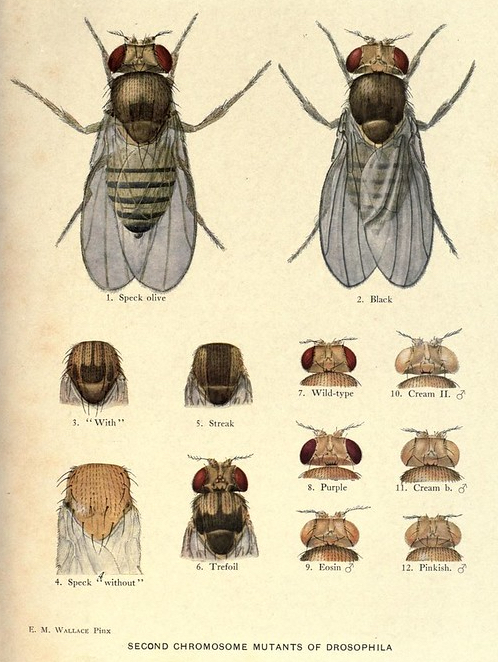
\includegraphics[width= 0.8 \textwidth]{illustration_images/alleles_genotypes/Drosophila_mel/Drosophila_mel_mutants.jpg}
\end{center}
\caption{ {\it Drosophila melanogaster} holds a special place in the
  history of genetics and population genetics. From Morgan's fly room discovering the principals of genetics to Dobzhansky's early work
  on natural genetic variation.  \BHLNC{Contributions to the genetics of Drosophila melanogaster
    (1919). Morgan T.H., Bridges C.B., Sturtevant A. H.}{https://www.biodiversitylibrary.org/page/805594\#page/147/mode/1up}{MBLWHOI Library} } \label{fig:dros}
\end{marginfigure}



Table \ref{Table:ADH} shows a small stretch of orthologous sequence for
the ADH locus from samples from {\it Drosophila melanogaster},  {\it D. simulans},
and {\it D. yakuba}.  {\it D. melanogaster} and {\it D. simulans} are
sister species and  {\it D. yakuba} is a close outgroup to the two.  Each column represents a single haplotype from an
individual (the individuals are diploid but were inbred so they're
homozygous for their haplotype). Only sites that differ among
individuals of the three species are shown. Site $834$ is an example
of a polymorphism; some  {\it D. simulans} individuals carry a $C$
allele while others have a $T$. \emph{Fixed differences}  are sites that differ between the species but are monomorphic within
  the species. Site $781$ is an example of a fixed difference between
  {\it D. melanogaster} and the other two species.

We can also annotate the alleles and loci in various ways. For example, position
$781$ is a non-synonymous fixed difference. We call the less common
allele at a polymorphism the  \emph{minor allele} and the common
allele the \emph{major allele}, e.g. at site $1068$ the $T$ allele is the
minor allele in {\it D. melanogaster}. We call the more evolutionarily
recent of the two alleles the \emph{derived allele} and the older of
the two the \emph{ancestral allele}. We infer that the $T$ allele at site 1068 is
the derived allele because the $C$ is found in both other species,
suggesting that the $T$ allele arose via a $C \rightarrow T$ mutation.

% For example, at a particular nucleotide site in the genome, a population may segregate for A-T and G-C base pairs (note that due to the complementary nature of DNA, it will suffice to say the site segregates for A and G variants).

\begin{table*}
  \tiny
\setlength{\tabcolsep}{.45\tabcolsep}   % https://tex.stackexchange.com/questions/307770/centered-tabular-column-with-narrow-columns
 %\csvreader[tabular=c]{Journal_figs/alleles_genotypes/ADH_MK/ADH.csv}
\csvautobooktabular{Journal_figs/alleles_genotypes/ADH_MK/ADH.csv}  % can control this more https://mirror.hmc.edu/ctan/macros/latex/contrib/csvsimple/csvsimple.pdf
  \caption{Variable sites in exons 2 and 3 of the ADH gene in {\it Drosophila} \citet{mcdonald:91}.
The first column (pos.) gives the position in the gene; exon 2 begins at
position $778$ and we've truncated the dataset at site $1175$.
The second column gives the consensus nucleotide (con.), i.e. the most
common base at that position; individuals with nucleotides that match
the consensus are marked with a dash.  The first columns of sequence
(a-l) are from {\it D. melanogaster};
    the next columns (a-f) give sequences from \textit{D. simulans}, and the final
 set of columns (a-l ) from {\it D. yakuba}. The last column shows
 whether the difference is a non-synonymous (N) or synonymous (S) change. }  % I've dropped the
                                % heterozygote sites from D. yakuba.
  \label{Table:ADH}
\end{table*}

\begin{question}
{\bf A)} How many segregating sites does the sample from \textit{
  D. simulans} have in the ADH gene?\\
{\bf B)} How many fixed differences are there between \textit{D. melanogaster} and \textit{D. yakuba}?
%What is the per base divergence are there between {\emph D. melanogaster} and {\emph D. yakuba}?
\end{question}
%JRI: confusing because site 974 is tri-allelic so "fixed" for derived allele but...

\section{Allele frequencies}
Allele frequencies are a central unit of population genetics
analysis, but from diploid individuals we only get to observe genotype
counts. Our first task then is to calculate allele frequencies from
genotype counts. Consider a diploid autosomal locus segregating for two alleles ($A_1$ and
$A_2$). We'll use these arbitrary labels for our alleles, merely to keep this
general. Let $N_{11}$ and $N_{12}$ be the number of $A_1A_1$ homozygotes and
$A_1A_2$ heterozygotes, respectively. Moreover, let $N$ be the total number of
diploid individuals in the population. We can then define the relative
frequencies of $A_1A_1$ and $A_1A_2$ genotypes as $f_{11} = N_{11}/N$ and
$f_{12} = N_{12}/N$, respectively. The frequency of allele $A_1$ in the
population is then given by

\begin{equation}
  p = \frac{2 N_{11} + N_{12}}{2N} = f_{11} + \frac{1}{2} f_{12}.
\end{equation}
Note that this follows directly from how we count alleles given individuals'
genotypes, and holds independently of Hardy--Weinberg proportions and
equilibrium (discussed below). The frequency of the alternate allele ($A_2$) is
then just $q=1-p$.

\subsection{Measures of genetic variability}
\paragraph{Nucleotide diversity ($\pi$)}
One common measure of genetic diversity is the average number of single
nucleotide differences between haplotypes chosen at random from a
sample. This is called \emph{nucleotide diversity} and is often denoted by
$\pi$.
For example, we can calculate $\pi$ for our ADH locus from Table \ref{Table:ADH} above: we have
6 sequences from \textit{D. simulans}  (a-f), there's a total of 15 ways of pairing
these sequences, and
\begin{equation}
\pi=\frac{1}{15} \big( (2 + 1 + 1 + 1 + 0 ) + (3 + 3 + 3 + 2 ) +(0 + 0 + 1) + (0 + 1) + (1)  \big)=1.2\overline{6}
\end{equation}
where the first bracketed term gives the pairwise differences between
a and b-f, the second bracketed term the differences between b and c-f
and so on. \\

Our $\pi$ measure will depend on the length of sequence it is calculated
for. Therefore, $\pi$ is usually normalized by the length of sequence,
to be a per site (or per base) measure. For example, our ADH sequence covers $397$bp of DNA and so $\pi = 1.2\overline{6}/397=0.0032$ per site in \textit{D. simulans} for this region. Note that we could also calculate $\pi$ per synonymous site (or non-synonymous). For synonymous site $\pi$, we would count up number of synonymous differences between our pairs of sequences, and then divide by the total number of sites where a synonymous change could have occurred.{\sidenote{Technically we would need to divide by the total number of possible point mutations that would result in a synonymous change; this is because some mutational changes at a particular nucleotide will result in a non-synonymous or synonymous change depending on the base-pair change.}


\paragraph{Number of segregating sites.} Another measure of genetic variability is the total number of sites
that are polymorphic (segregating) in our sample. One issue is that
the number of segregating sites will grow as we sequence more
individuals (unlike $\pi$). Later in the course, we'll talk about how to standardize the
number of segregating sites for the number of individuals sequenced (see eqn \eqref{watterson_theta}).

\paragraph{The frequency spectrum.}
We also often want to compile information about the frequency of
alleles across sites.  We call alleles that are found once in a sample
\emph{singletons}, alleles that are found twice in a sample {\emph
  doubletons}, and so on. We count up the number of loci where an
allele is found $i$ times out of $n$, e.g. how many singletons are
there in the sample, and this is called the \emph{frequency
  spectrum}. We'll want to do this in some consistent manner, such as calculating the frequency spectrum of the minor allele or the derived allele.

\begin{question}
How many minor-allele singletons are there in \textit{D. simulans} in
the ADH region? [Defining minor allele just within \textit{D. simulans}.]
%JRI: ambiguous. is the minor allele defined across all species or just within simulans?
\erin{students were confused whether you are defining 'minor allele' with reference to the species or to the whole group. There are no major allele singletons with reference to the individual species, but I think it's confusing because the only example of a minor allele given in the text by its definition is the 'minor allele in D. melanogaster' .. maybe it would be best to clarify in the question or just give an example of the minor allele in the whole sample instead.}
 \end{question}
\paragraph{Levels of genetic variability across species.}
Two observations have puzzled population geneticists since the
inception of molecular population genetics. The first is the relatively high
level of genetic variation observed in most obligately sexual species.
This first observation, in part, drove the development of the Neutral
theory of molecular evolution, the idea that much of this molecular
polymorphism may simply reflect a balance between genetic drift and
mutation.
The second observation is the relatively narrow range of
polymorphism across species with vastly different census sizes. This
observation represented a puzzle as the Neutral theory predicts that
levels of genetic diversity should scale with population size. Much effort
in theoretical and empirical population genetics has been devoted to
trying to reconcile models with these various observations. We'll
return to discuss these ideas throughout our course.
%Neutral

\begin{marginfigure}[-1cm]
\begin{center}
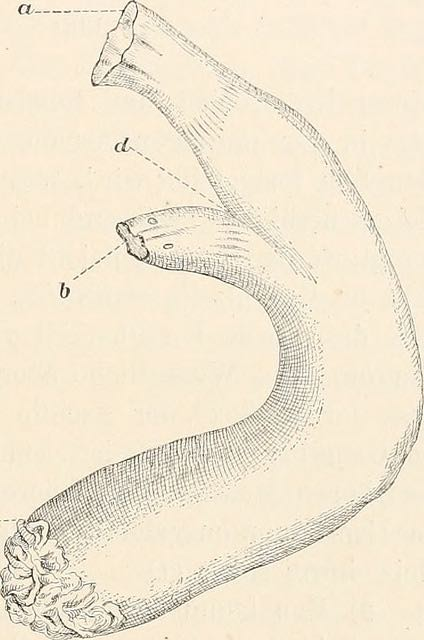
\includegraphics[width= 0.8 \textwidth]{illustration_images/alleles_genotypes/Ciona_intestinalis/21016139168_2a8a57ded3_z.jpg}
\end{center}
\caption{Sea Squirt ({\it Ciona intestinalis}). \BHLNKC{Einleitung in die vergleichende gehirnphysiologie und
  Vergleichende psychologie. Loeb, J. 1899.}{https://www.flickr.com/photos/internetarchivebookimages/21016139168/in/photolist-y28cZ3-xatkQu-w6Ki9C-wLcTJy-tLanR7-wKRZbh-w79C6u-toKNq1-u3ojn3-y8KsPP-xK7CZj-bu2usR-wLkfdM-wbkfau-x8n51o-ygpRAN-xMgGnk-towSTe-xQtix3-xMrift-wQoMNq-y51RxU-xPH4Cu-x4uB1v-xPGVFs-x4GN5a-y6rT8N-y6Aous-y7jV9n-yb6s66-x7F6Wh-y7upRp-xkz9VY-u1qerd-wYE4Cz-y5aH2Y-y7uJpM-xPSvFU-y6ALo7-xPZ3FM-xPHUef-yaa3dw-xPSKSC-w7A1aj-x4bgsH-tLas4q-x1e1dv-w7BkZB-xrQxFJ-y8acDr}{MBLWHOI Library}} \label{fig:ciona}
\end{marginfigure}

The first observations of molecular genetic diversity within natural populations were made from surveys of allozyme data, but we can revisit these general patterns with modern data. \\
\begin{figure*}
\begin{center}
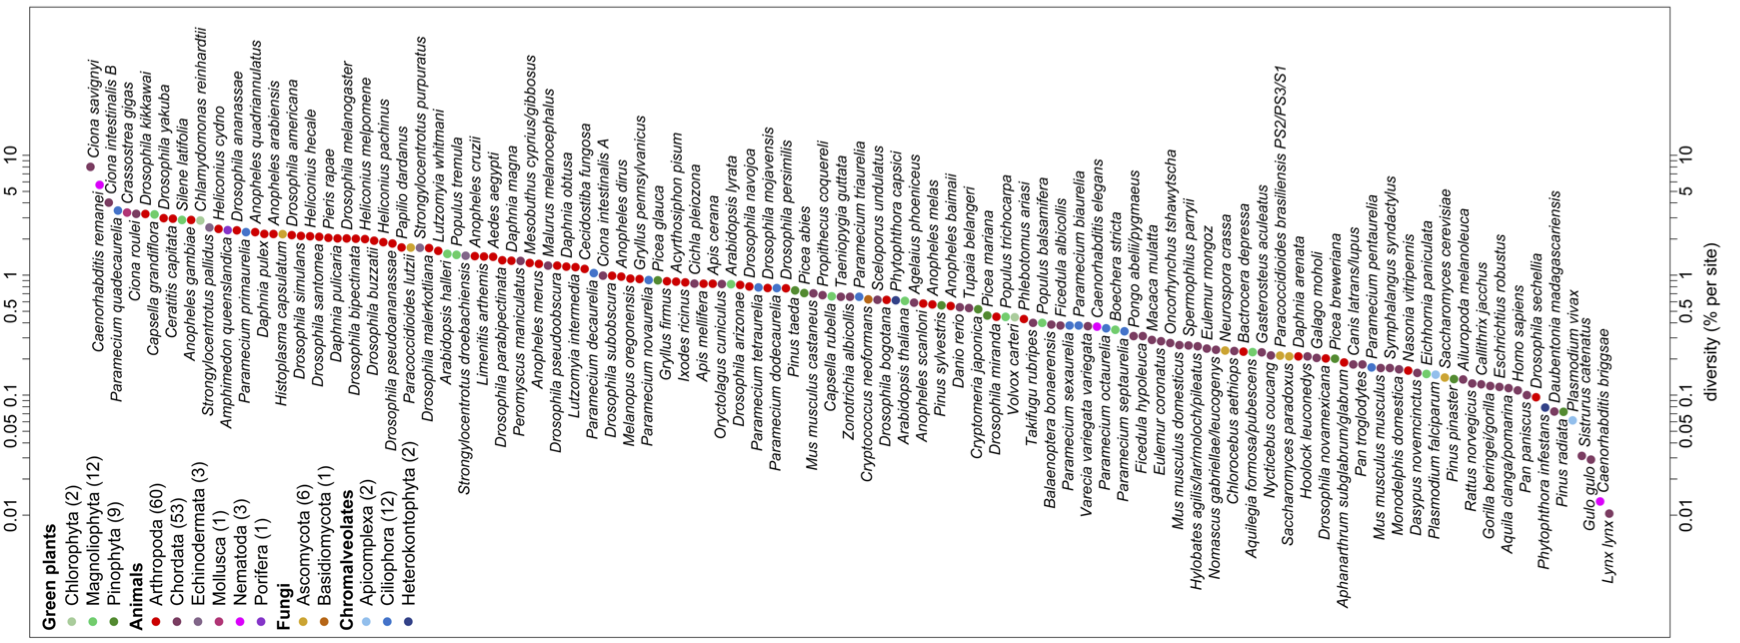
\includegraphics[width= \textwidth]{Journal_figs/alleles_genotypes/Leffer_riddle/Leffer_riddle_diversity.png}
\end{center}
\caption{Levels of autosomal nucleotide diversity for 167
species across 14 phyla. Figure 1 from \citet{leffler:12}, \PLOSccBY. Points are
ranked by their $\pi$, and coloured by their phylum. Note the log-scale.} \label{fig:Leffer}
\end{figure*}
For
example, \citet{leffler:12} compiled data on levels of within-population,
autosomal nucleotide diversity ($\pi$) for 167 species across 14 phyla from
non-coding and synonymous sites (Figure \ref{fig:Leffer}). The species with the lowest levels of
$\pi$ in their survey was Lynx, with $\pi = 0.01\%$, i.e. only
$1/10000$ bases differed between two sequences. In contrast, some of the highest levels of
diversity were found in {\textit{Ciona savignyi}, Sea Squirts, where a remarkable
$1/12$ bases differ between pairs of sequences. This $800$-fold range of
diversity seems impressive, but census population sizes have a much
larger range.
%JRI: I feel like an example of census size would be useful. the genus Cyclothone, which exists in the trillions, comes to mind as a surprising example that you could compare to like a coelocanth: https://commons.wikimedia.org/wiki/File:Wissenschaftliche_Ergebnisse_der_Deutschen_Tiefsee-Expedition_auf_dem_Dampfer_%22Valdivia%22_1898-1899_(Tafel_6)_(7413855904).jpg

\begin{marginfigure}[2cm]
\begin{center}
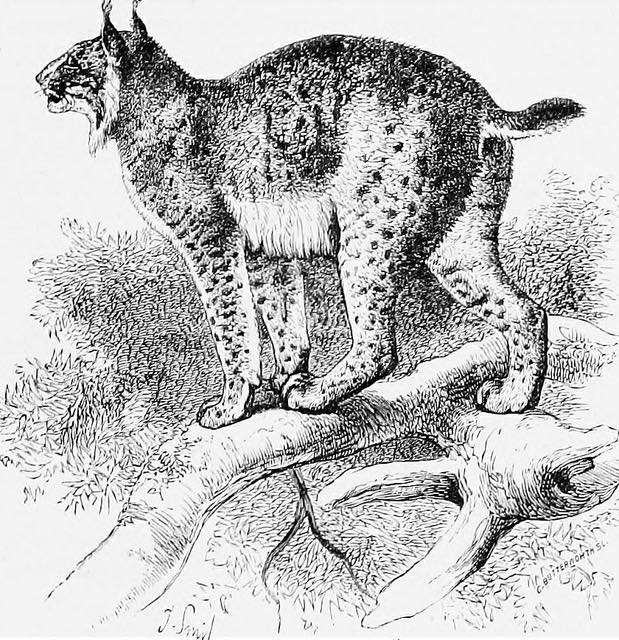
\includegraphics[width= 0.8 \textwidth]{illustration_images/alleles_genotypes/Lynx/20731949565_8a065700af_z.jpg}
\end{center}
\caption{Eurasian Lynx (\textit{Lynx lynx}). \BHLNKC{An introduction to the study
  of mammals living and extinct. Flower, W.H. and Lydekker, R. 1891.}{https://www.flickr.com/photos/internetarchivebookimages/20731949565/in/photolist-x5Jzv2-x6QVyp-xir9rH-wYHrQD-wPn1sP-w9PsqY-xDcqri-sMcQoB-trrkVd-x6Nx1H-wPea7N-sM28N9-tJ3zsp-xneVdx-wGJRtQ-xnfHZ8-wPfga7-xCUPrN-x7kXDV-xmAb9E-xm3x4k-xBoSKb-wGTgyB-xBoSbf-wGGvzA-xmzYTJ-oeKJcH-xA1Ffr-xA1Eji-xqWTQZ-xF4Lru-oxJfrH-x7ojSn-xra8zP-wGGibY-xgb21y-xY1jH9-xY1iyf-wGHxTS-wGQEoR-xmtPQh-x8uFKK-xdTkoU-wPggQf-wPfvHN-wPfc27-w9YnGF-wPeauS-wPiVxK-w6aiSi}{Cornell University Library}} \label{fig:Lynx}
\end{marginfigure}

\subsection{Hardy--Weinberg proportions}
Imagine a population mating at random with respect to genotypes, i.e. no
inbreeding, no assortative mating, no population structure, and no sex differences
in allele frequencies. The frequency of allele $A_1$ in the population at the
time of reproduction is $p$. An $A_1A_1$ genotype is made by reaching out into
our population and independently drawing two $A_1$ allele gametes to form a
zygote. Therefore, the probability that an individual is an $A_1A_1$ homozygote
is $p^2$. This probability is also the expected frequencies of the $A_1A_1$
homozygote in the population. The expected frequency of the three possible
genotypes are

\marginnote{Throughout this chapter we'll be making use of the basic
  rules of probability to find the probabilities of combinations of
  events, e.g. the alleles found in an individual, see Appendix \ref{Section_rules_prob} for a refresher.}

%\begin{table}[htp!]
\begin{center}
\begin{tabular}{ccc}
\hline
$f_{11}$ & $f_{12}$ & $f_{22}$ \\
\hline
$p^2$ & $2pq$ & $q^2$ \\
\end{tabular}
\end{center}
%\caption{\textbf{Hardy Weinberg}} \label{table:HWE}
%\end{table}
Note that we only need to assume random mating with respect to our focal allele in order for these expected frequencies to hold in the zygotes forming the next generation. Evolutionary forces, such as selection, change allele frequencies within generations, but do not change this expectation for new zygotes, as long as $p$ is the frequency of the $A_1$ allele in the population at the time when gametes fuse.
%\erin{I wasn't sure what contrast you were getting at here, so may not be a good edit}

\begin{question}
On the coastal islands of British Columbia there is a subspecies of
black bear (\textit{Ursus americanus kermodei}, Kermode's bear). Many members of this
black bear subspecies are white; they're sometimes called spirit bears. These
bears aren't hybrids with polar bears, nor are they albinos. They are
homozygotes for a recessive change at the MC1R gene. Individuals who
are $GG$ at this SNP are white while $AA$ and $AG$ individuals are black.



\begin{marginfigure}    %%%New Kermode_bear
                        %%%https://twitter.com/BioDivLibrary/status/1191354772034592774/photo/3
                        %%%page 77 https://www.biodiversitylibrary.org/item/38166?utm_source=Twitter&utm_medium=social+media&utm_term=&utm_content=MBLWHOI&utm_campaign=Mammal+Monday#page/114/mode/1up
  \begin{center}
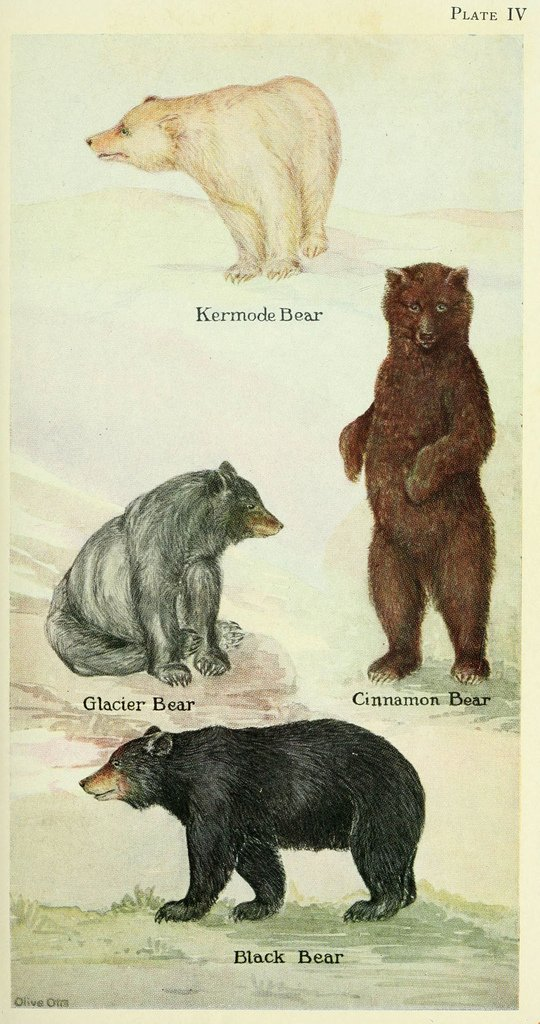
\includegraphics[width= \textwidth]{illustration_images/alleles_genotypes/Kermode_bear/EIiK2dsWoAAmUOf.jpeg}  
%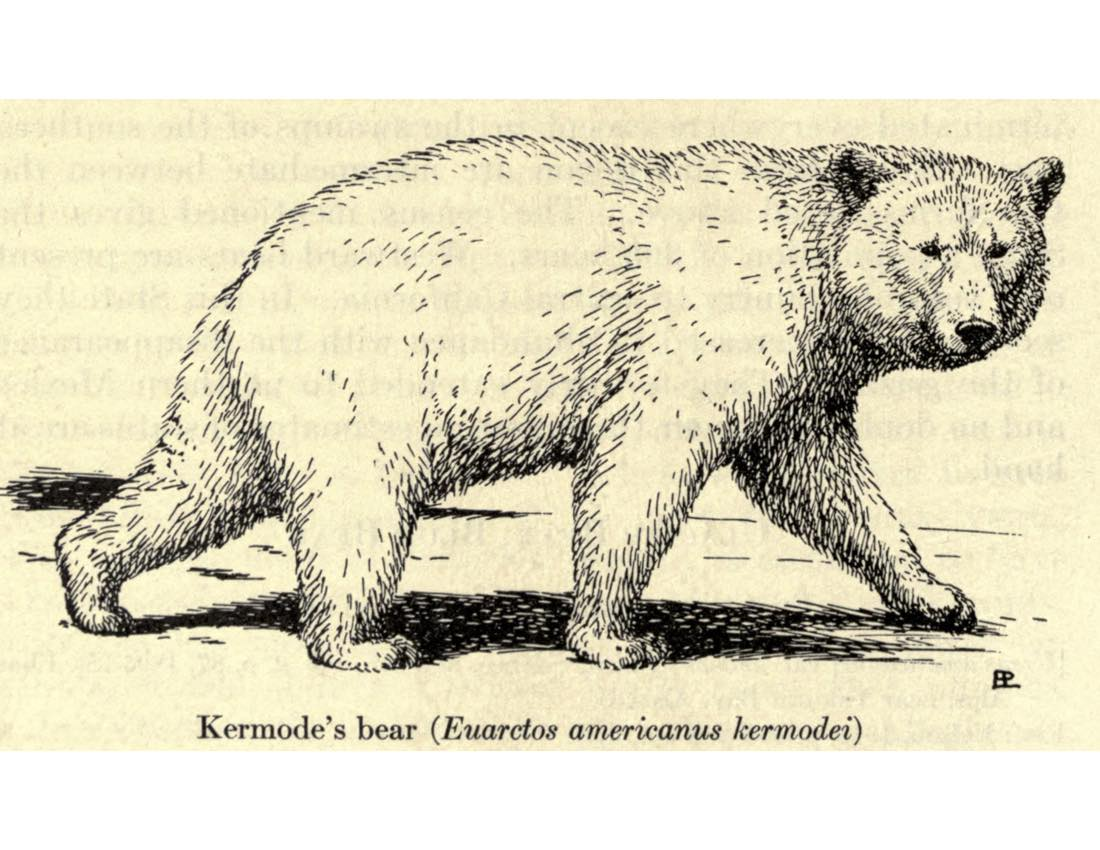
\includegraphics[width= \textwidth]{illustration_images/alleles_genotypes/Kermode_bear/Kermode_bear.jpg}
\end{center}
\caption{Kermode's bear (\textit{Ursus americanus kermodei}). It's
  possible that this morph is favoured as the salmon these bears eat have a harder time
  seeing the light morph \citep{klinka2009adaptive}. The adaptive
  value of tasting like cinnamon is unknown. \BHLNKC{Field book of North American mammals;
    descriptions of every mammal known north of the Rio
    Grande. Anthony, (1928) H. E.}{https://www.biodiversitylibrary.org/item/38166\#page/115/mode/1up}{MBLWHOI Library} } \label{fig:Kermodes_bear}
%\caption{Kermode's bear. \BHLNC{Extinct and vanishing mammals of the western
 % hemisphere. 1942. Glover A.}{https://www.biodiversitylibrary.org/page/20699033\#page/160/mode/1up}{Prelinger
%  Library} } \label{fig:Kermodes_bear}
\end{marginfigure}

Below are the genotype counts for the MC1R polymorphism in a
sample of bears from British Columbia's island populations from \citet{RITLAND:01}.
\begin{center}
\begin{tabular}{ccc}
\hline
$AA$ & $AG$ & $GG$ \\
\hline
42 & 24 & 21\\
\end{tabular}
\end{center}
What are the expected frequencies of the three genotypes under HWE?
\end{question}
%JRI: I think you mean under HW not HWE.  i think somewhere you should introduce HW in a parenthetical"Hard--Weinberg  (HW) proportions" etc. just to be abdunantly clear what the acronym means. also the ritland citation isn't showing year for some reason.


See Figure \ref{fig:HWE_CEU_YRI} for a nice
empirical demonstration of Hardy--Weinberg proportions. The mean
frequency of each genotype
closely matches its HW expectations, and much of the scatter of the
dots around the expected line is due to our small sample size ($\sim
60$ individuals). While HW often
seems like a silly model, it often holds remarkably well within
populations. This is because individuals don't mate at random, but they
do mate at random with respect to their genotype at most of the loci
in the genome.

\begin{figure}[!h]
\begin{center}
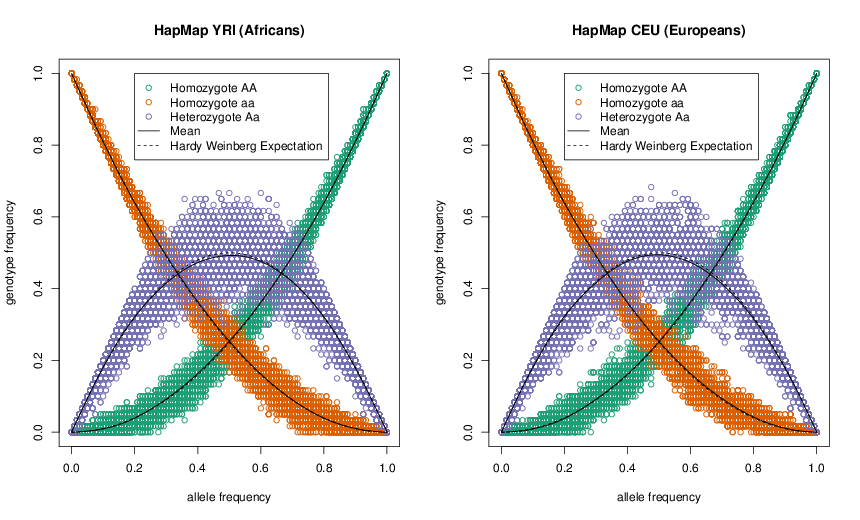
\includegraphics[width= \textwidth]{figures/CEU_YRI_separately_HWE.png}
\end{center}
\caption{Demonstrating Hardy--Weinberg proportions using 10,000 SNPs
  from the HapMap European (CEU)  and African (YRI) populations. Within
  each of these populations the allele frequency against the
  frequency of the 3 genotypes; each SNP is represented by 3 different
  coloured points. The solid lines show the mean genotype frequency. The dashed lines show the
  predicted genotype frequency from Hardy--Weinberg
  equilibrium. \gitcode{https://github.com/cooplab/popgen-notes/blob/master/Rcode/HWE_exercise/HWE_HAPMAP.R} Blog
  post on figure \href{http://gcbias.org/2011/10/13/population-genetics-course-resources-Hardy--Weinberg-eq/}{here}. } \label{fig:HWE_CEU_YRI}  %See \href{blog
                                %post}{http://gcbias.org/2011/10/13/population-genetics-course-resources-Hardy--Weinberg-eq/}
                                %here on this plot.  https://github.com/cooplab/popgen-notes/blob/master/Rcode/HWE_exercise/HWE_HAPMAP.R
\end{figure}

\begin{question}
You are investigating a locus with three alleles, A, B, and C, with
allele frequencies $p_A$, $p_B$, and $p_C$. What fraction of the
population is expected to be homozygotes under Hardy--Weinberg?
\end{question}

Microsatellites are regions of the genome where individuals vary for
the number of copies of some short DNA repeat that they carry. These
regions are often highly variable across individuals, making them
a suitable way to identify individuals from a DNA sample. This
so-called DNA fingerprinting has a range of applications from
establishing paternity and identifying human remains to matching
individuals to DNA samples from a crime scene. The FBI make use of the
CODIS database\sidenote{CODIS: Combined DNA Index System}. The CODIS
database contains the genotypes of over 13 million people, most of
whom have been convicted of a crime. Most of
the profiles record genotypes at 13 microsatellite loci that are
tetranucleotide repeats (since 2017, 20 sites have been genotyped).

The allele counts for two loci (D16S539
and TH01) are shown in table \ref{table:CODIS_1} and
\ref{table:CODIS_2} for a sample of 155 people of European ancestry. You can assume these two loci are on different chromosomes.

\begin{table}
{\small
\setlength{\tabcolsep}{.45\tabcolsep}
\csvautobooktabular{Rcode/CODIS/D16S539_counts.csv}  \label{table:CODIS_1}
\caption{ Data for 155 Europeans at the D16S539 microsatellite from
  CODIS from \citet{algee:16}. The top row gives the number of
  tetranucleotide repeats for each allele, the bottom row gives the
  sample counts.}
 }

\end{table}
\vspace*{1cm}
\begin{table}
  {\small
\setlength{\tabcolsep}{.45\tabcolsep}
\csvautobooktabular{Rcode/CODIS/TH01_counts.csv}  \label{table:CODIS_2}
}

\caption{Same as \ref{table:CODIS_1} but for the TH01 microsatellite. }
\end{table}

\begin{question} \label{Q:CODIS}
You extract a DNA sample from a crime scene. The genotype is 100/80 at the
D16S539 locus and 70/93 at TH01.\\

{\bf A)} You have a suspect in custody. Assuming this suspect is innocent and of European ancestry, what is the probability
that their genotype would match this profile by chance (a false-match probability)?\\
{\bf B)} The FBI uses $\geq 13$ markers. Why is this higher number
necessary to make the match statement convincing evidence in court?\\
{\bf C)}  An early case that triggered debate among forensic geneticists was a crime among the Abenaki, a Native American community in
Vermont \citep[see ][ for discussion]{lewontin:94}. There was a DNA sample from the crime scene, and the
perpetrator was thought likely to be a member of the Abenaki
community. Given that allele frequencies vary among populations, why would people be concerned about using data from a non-Abenaki population to compute a false match probability?
%---that is, the probability
%that a suspect's DNA would match a crime-scene sample if he were unrelated to anyone present at the crime scene
\end{question}

%\begin{question}
%Suppose the following genotype frequencies were observed for at an esterase locus in a population of Drosophila (A denotes the “fast” allele and B denotes the “slow” allele):
%\begin{center}
%\begin{tabular}{|ccc|}
%AA &	AB &	BB\\
%0.6 &	0.2 &	0.2\\
%\end{tabular}\,.
%\end{center}
%What genotype frequencies would you expect under Hardy Weinberg expectations?
%\end{question}


%%%ADD A comment about WF sampling here!
%% Also add a question about Poisson offspring number.

%\begin{figure}
%\begin{center}
%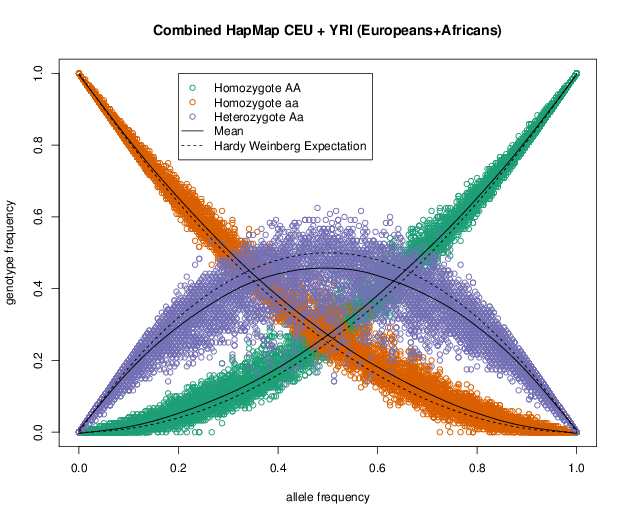
\includegraphics[width=0.5 \textwidth]{figures/CEU_YRI_together_HWE.png}
%\end{center}
%\caption{}
%\end{figure}


%figure/QT1.eps

\section{Allele sharing among related individuals and Identity by Descent}

All of the individuals in a population are related to each other by a giant
pedigree (family tree). For most pairs of individuals in a population these
relationships are very distant (e.g. distant cousins), while some individuals
will be more closely related (e.g. sibling/first cousins). All individuals
are related to one another by varying levels of relatedness, or \emph{kinship}.
Related individuals can share alleles that have both descended from the shared
common ancestor. To be shared, these alleles must be inherited through all
meioses connecting the two individuals (e.g. surviving the $\nicefrac{1}{2}$
probability of segregation each meiosis). As closer relatives are separated by
fewer meioses, closer relatives share more alleles. In Figure
\ref{fig:IBD_cousins_chr_cartoon} we show the sharing of chromosomal regions
between two cousins. As we'll see, many population and quantitative genetic
concepts rely on how closely related individuals are, and thus we need some way
to quantify the degree of kinship among individuals. \\
\begin{figure}
\begin{center}
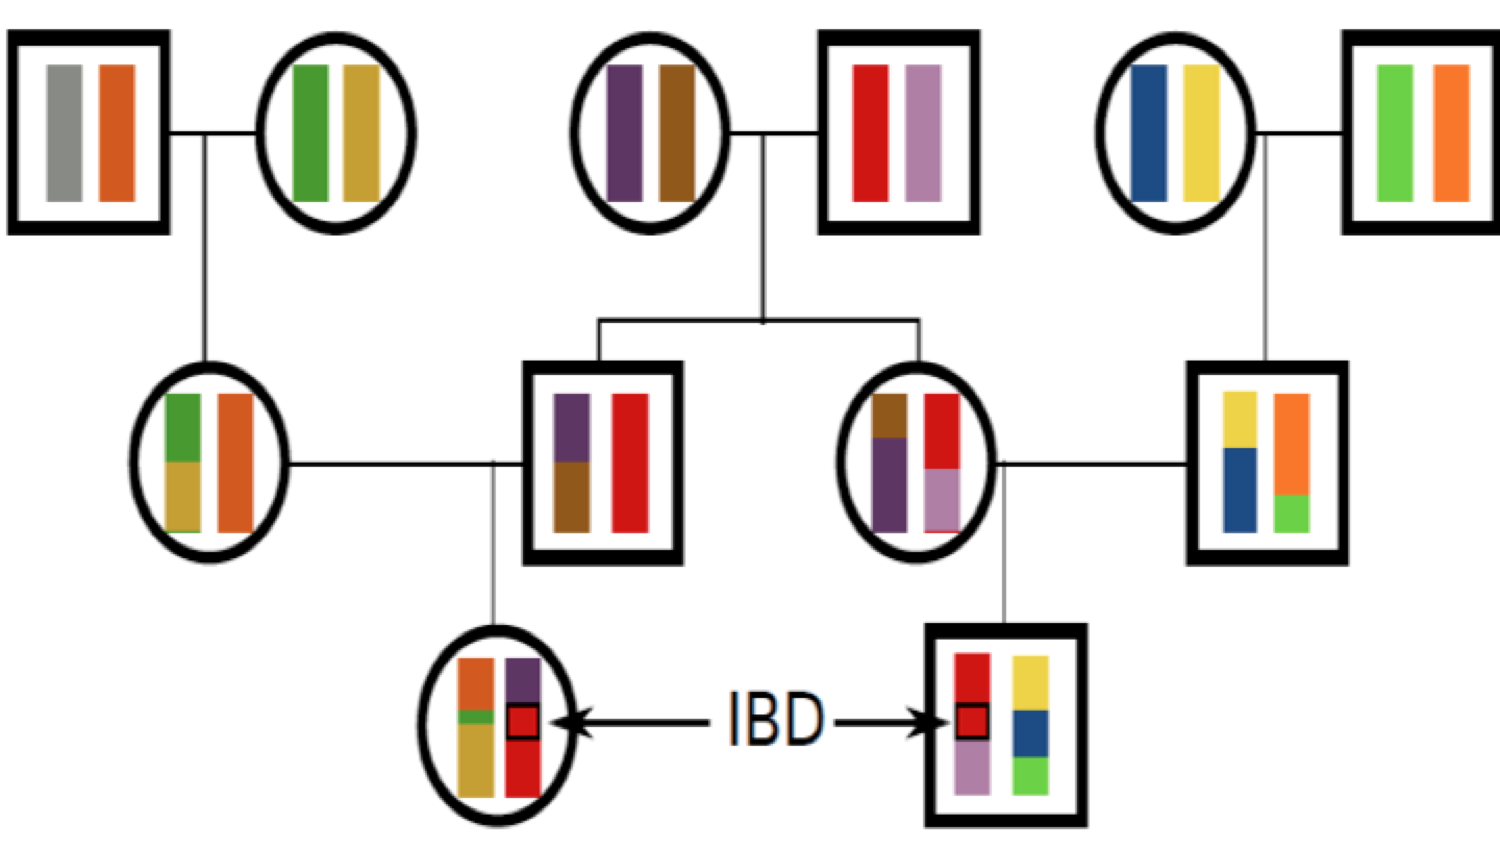
\includegraphics[width= 0.75 \textwidth]{figures/Cousins_IBD_chromo_cartoon.png}
\end{center}
\caption{First cousins sharing a stretch of chromosome identical by
  descent. The different grandparental diploid chromosomes are coloured so we
  can track them and recombinations between them across the
  generations. Notice that the identity by descent between the cousins persists for a long
stretch of chromosome due to the limited number of generations for
recombination. The squares represent males and circles females. } \label{fig:IBD_cousins_chr_cartoon}
\end{figure}

We will define two alleles to be identical by descent (IBD) if they are
identical due to transmission from a common ancestor in the past few generations\cite{cotterman:40,malecot:48}. For the moment,
we ignore mutation, and we will be more precise about what we mean by `past few
generations' later on. For example, parent and child share exactly one allele
identical by descent at a locus, assuming that the two parents of the child are
randomly mated individuals from the population. In Figure
\ref{fig:IBD_cousins_cartoon}, I show a pedigree demonstrating some
configurations of IBD. \\

\marginnote{Here we'll focus on IBD of outbred individuals. Dealing
  with sharing between inbred individuals requires $6$ more  identity-by-descent
$r$ coefficients, which honestly makes my head spin.}
One summary of how related two individuals are is the probability that our pair
of individuals share 0, 1, or 2 alleles identical by descent (see Figure
\ref{fig:IBD_0_1_2}). We denote these  identity-by-descent probabilities by $r_0$, $r_1$, and $r_2$
respectively. See Table \ref{table:IBDprobs} for some examples. We can also
interpret these probabilities as genome-wide averages. For example, on average, at a quarter of all their autosomal loci
full-sibs share zero alleles identical by descent.\\



One summary of relatedness that will be important is the probability that two
alleles ($I$ \& $J$) picked at random, one from each of the two different individuals $i$
and $j$, are identical by descent ($P(\text{I\&J IBD})$). We call this quantity the \emph{coefficient
of kinship} of individuals $i$ and $j$, and denote it by $F_{ij}$. It is
calculated as
%JRI: you come back to inbreeding later, but perhaps worth mentioning here that you are only considering outbred Individuals

\begin{align}
  F_{ij} = & P(\text{I\&J IBD} )\\
  =& P(\text{I\&J IBD} |~ \text{i\&j  0 IBD}) P(\text{i\&j  0 IBD})  \nonumber\\
  & + P(\text{I\&J IBD} |~ \text{i\&j  1 IBD})
    P(\text{i\&j  1 IBD})  \nonumber\\
  &+ P(\text{I\&J IBD} |~ \text{i\&j  2 IBD}) P(\text{i\&j  2 IBD}) \label{eqn:coeffkinship_step}\\
   =   &   0 \times r_0 + \frac{1}{4} r_1  + \frac{1}{2} r_2.
\label{eqn:coeffkinship}
\end{align}
\begin{marginfigure}[-1cm]
\begin{center}
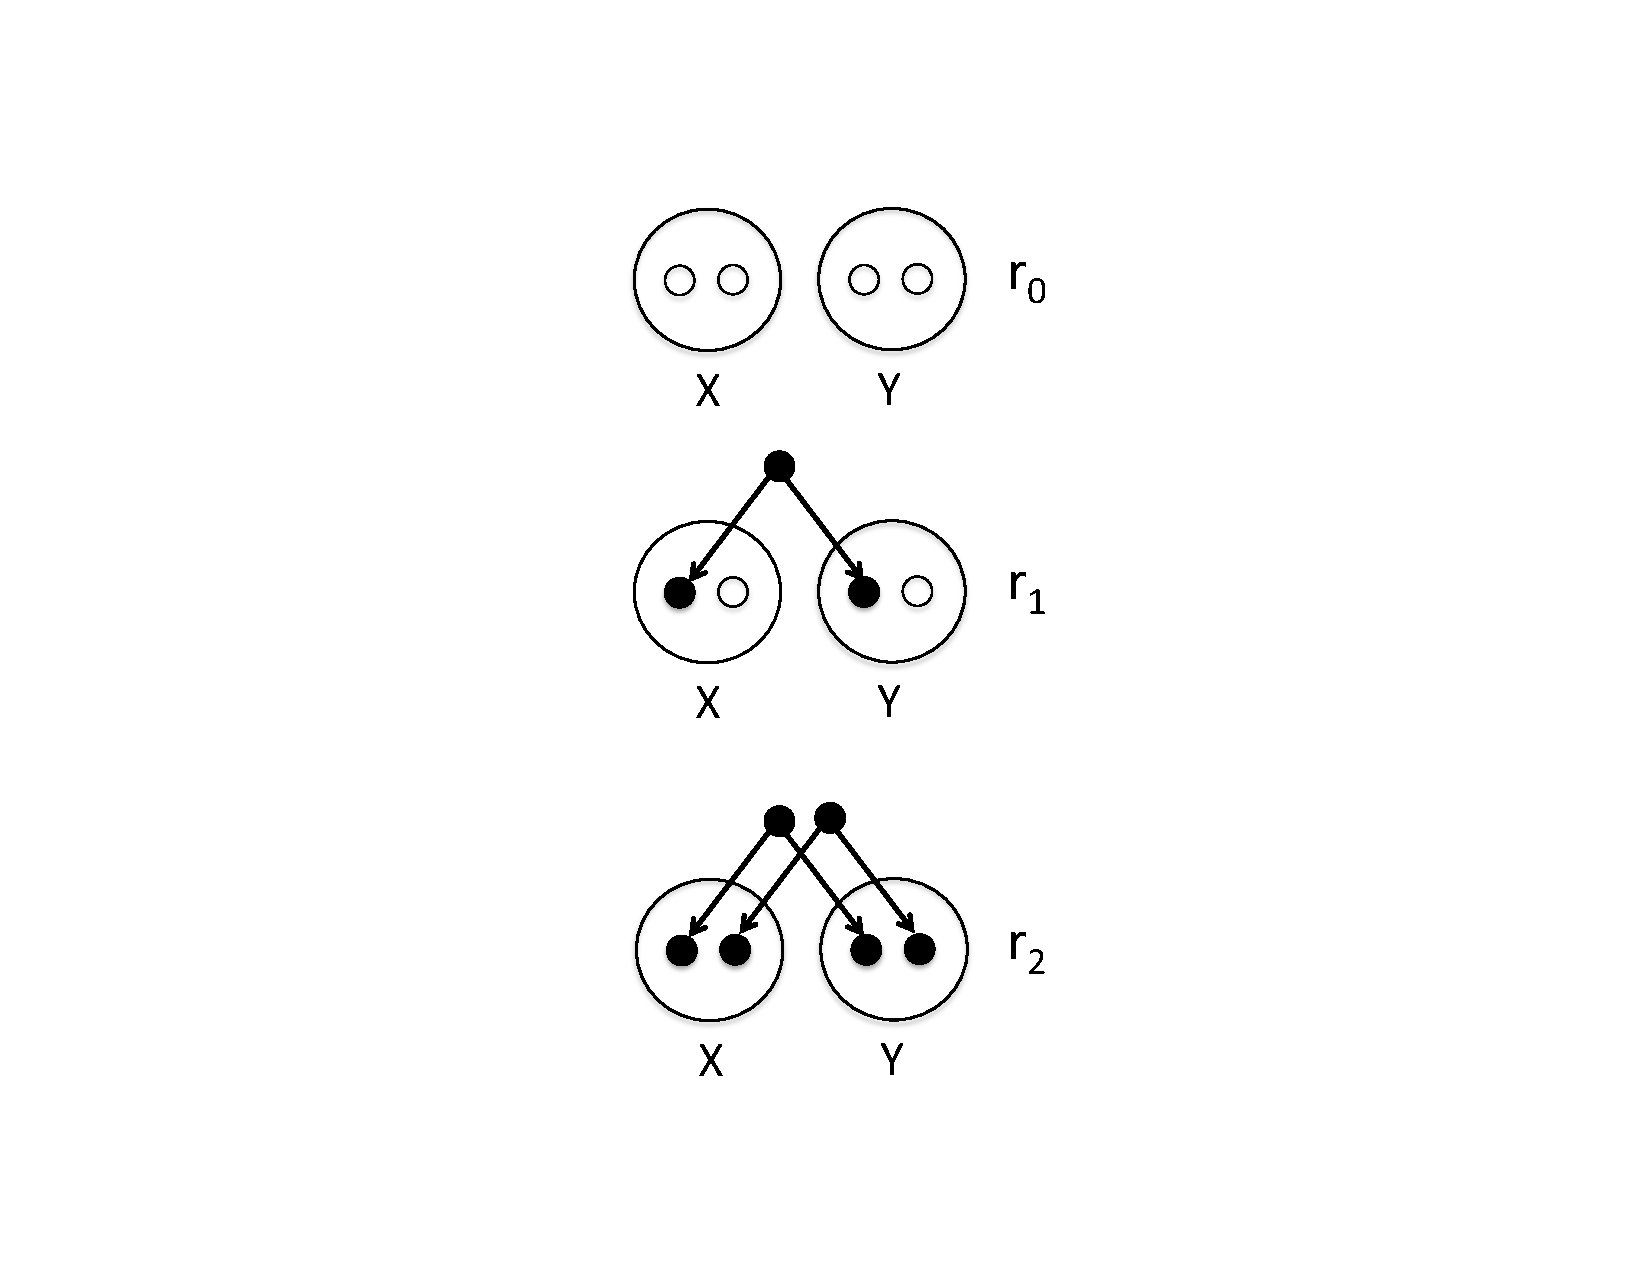
\includegraphics[width= 0.75 \textwidth]{figures/sharing_relatives/IBD_0_1_2.pdf}
\end{center}
\caption{A pair of diploid individuals (i and j) sharing 0, 1, or 2 alleles IBD
  where lines show the sharing of alleles by descent (e.g. from a
  shared ancestor). } \label{fig:IBD_0_1_2}
\end{marginfigure}

In the above step, eqn\eqref{eqn:coeffkinship_step}, we're summing the
conditional probability of alleles $I$ \& $J$ being IBD over whether our individuals $i$ \& $j$ share $0$, $1$,
or $2$ alleles IBD, an example of using the Law of Total Probability (see Appendix
eqn \eqref{eqn:law_tot_prob}).  We've then, in eqn \ref{eqn:coeffkinship}, used the fact that we can
calculate our condition probabilities of  I \& J being IBD using the
rules of Mendelian transmision. Consider the probability $
P(\text{I\&J IBD} |~ \text{i\&j  1 IBD})$, i.e. that our
pair of alleles ($I$ \& $J$) drawn from individuals $i$ and $j$ are IBD given that
$i$ and $j$ share one allele IBD, this is a $\nicefrac{1}{4}$ as we need to
draw the allele that is IBD from both $i$ and $j$, i.e. drawing both black
alleles in the middle panel of Figure \ref{fig:IBD_0_1_2}, which
happens with probability $\nicefrac{1}{2} \times \nicefrac{1}{2} $. 
The coefficient of kinship will appear multiple times, in both our discussion of
inbreeding and in the context of phenotypic resemblance between relatives.\\

\begin{table*}
\begin{center}
\begin{tabular}{ l c c c c}
\hline
Relationship (i,j)$^{*}$ & $P(\text{i\&j  0 IBD}) $ & $P(\text{i\&j  1 IBD}) $ & $P(\text{i\&j  2 IBD}) $ & $P(\text{I\&J IBD} )$\\
  \hline
  Relationship (i,j)$^{*}$ & $r_0$ & $r_1$ & $r_2$ & $F_{ij}$\\
    \hline
parent--child & 0 & 1 & 0 & \nicefrac{1}{4}\\
full siblings & \nicefrac{1}{4} & \nicefrac{1}{2} & \nicefrac{1}{4} & \nicefrac{1}{4}\\
Monozygotic twins  & 0 & 0 & 1  & \nicefrac{1}{2} \\
$1^{st}$ cousins & \nicefrac{3}{4} & \nicefrac{1}{4} & 0 & \nicefrac{1}{16}\\
\hline
\end{tabular}
\end{center}
\caption{Probability that two individuals of a given relationship share 0, 1, or 2 alleles
identical by descent on the autosomes. $^{*}$Assuming that our
individuals are outbred and that this the only close relationship the pair shares. } % doesn't this implicitly assume an infinite population?
\label{table:IBDprobs}
\end{table*}

\begin{question}
  What are $r_0$, $r_1$, and $r_2$ for $\nicefrac{1}{2}$ sibs? ($\nicefrac{1}{2}$ sibs share one
parent but not the other).
\end{question}

\begin{question}
  Explain in words why $ P(\text{I\&J IBD} |~ \text{i\&j  2 IBD}) = \nicefrac{1}{2}$.
\end{question}

%Question 5. Consider a biallelic locus where allele 1 is at fre- quency p, and two individuals who have IBD allele sharing probabili- ties r0, r1, r2.
%What is the overall probability that these two individuals are both homozygous for allele 1?

\paragraph{Genotypic sharing between pairs of individuals.}
Our $r$ coefficients are going to have various uses. For example, they allow us
to calculate the probability of the genotypes of a pair of
relatives. Consider a biallelic locus where allele $A_1$ is
at frequency $p$, and two individuals who have IBD allele sharing
probabilities $r_0$, $r_1$, $r_2$. What is the overall probability that these
two individuals are both homozygous for allele 1? Well that's
\begin{align}
  P(A_1 A_1) = & P(A_1 A_1 | \text{0 alleles IBD}) P(\text{0 alleles IBD})  \nonumber\\
  & + P(A_1 A_1 | \text{1 allele IBD}) P(\text{1 allele IBD})  \nonumber\\
  &+ P(A_1 A_1 | \text{2 alleles IBD}) P(\text{2 alleles IBD})
\end{align}
Or, in our $r_0$, $r_1$, $r_2$ notation:
\begin{align}
  P(A_1 A_1) = & P(A_1 A_1 | \text{0 alleles IBD}) r_0  \nonumber\\
  & + P(A_1 A_1 |
  \text{1 alleles IBD}) r_1  \nonumber\\
  & + P(A_1 A_1 | \text{2 alleles IBD}) r_2 \label{eqn:initial_relly_IBD_calc}
\end{align}
If our pair of relatives share $0$ alleles IBD, then the probability that
they are both homozygous is $P(A_1 A_1 |
\text{0 alleles IBD}) =p^2 \times p^2$, as all four alleles
represent independent draws from the population. If they share $1$
allele IBD, then the shared allele is of type $A_1$ with probability $p$, and then
the other non-IBD allele, in both relatives, also needs
to be $A_1$ which happens with probability $p^2$, so $P(A_1 A_1 |
\text{1 alleles IBD})=p \times p^2$. Finally, our pair of relatives can
share two alleles IBD, in which case $P(A_1 A_1 | \text{2 alleles IBD})
= p^2$, because if one of our individuals is homozygous for the $A_1$ allele,
both individuals will be. Putting this all together our equation
\eqref{eqn:initial_relly_IBD_calc} becomes
\begin{equation}
P(A_1 A_1) = p^4 r_0 + p^3 r_1 + p^2 r_2 \label{eqn:IBD_relly_calc}
\end{equation}
Note that for specific cases we could also calculate this by summing over all the
possible genotypes their shared ancestor(s) had; however, that would be much more
involved and not as general as the form we have derived here.

We can write out terms like eq \eqref{eqn:IBD_relly_calc} for all of
the possible configurations of genotype
sharing/non-sharing between a pair of individuals. Based on this we can write down the expected number of
polymorphic sites where our individuals are observed to share 0, 1, or 2
alleles.

\begin{question} [Trickier question.]
The genotype of our suspect in Question \ref{Q:CODIS} turns out to be 100/80 for
D16S539 and 70/80 at TH01. The suspect is not a match to the DNA
from the crime scene; however, they could be a sibling.

Calculate the joint probability of observing the genotype from the crime and our
suspect:\\
{\bf A)} Assuming that they share no close relationship.\\
%JRI: pretty sure the answer key is wrong here. If we put your eact set of fractions into R we get 1.433992e-09 as the answer. So something is wrong somewhere in answer.

{\bf B)} Assuming that they are full sibs.\\

{\bf C)} Briefly explain your findings.
  \end{question}

 \begin{marginfigure}
\begin{center}
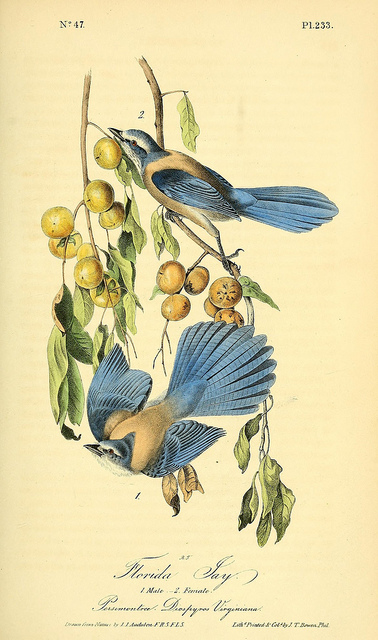
\includegraphics[width= \textwidth]{illustration_images/alleles_genotypes/Florida_scrub_jay/8576533889_3a131ffc4c_z.jpg}
\end{center}
\caption{Florida Scrub-Jays ({\it Aphelocoma coerulescens}). \BHLCC{The birds of America : from drawings made in the United
    States and their territories. 1880. Audubon
    J.J.}{https://www.biodiversitylibrary.org/page/40447048\#page/169/mode/1up}{Smithsonian
    Libraries}{2.0} } \label{fig:FSJ}
\end{marginfigure}


There's a variety of ways to estimate the relationships among
individuals using genetic data.  An example of using allele sharing to identify relatives is offered by
the work of Nancy Chen \citep[in collaboration with Stepfanie
Aguillon, see ][]{chen:16,Aguillon:17}. \citeauthor{chen:16} has collected genotyping data from thousands of
Florida Scrub Jays at over ten thousand loci. These Jays live at the
Archbold field site, and have been carefully monitored for many
decades allowing the pedigree of many of the birds to be known.
Using these data she estimates allele frequencies at each
locus. Then by equating the observed number of times that a pair of
individuals share $0$, $1$, or $2$ alleles to the theoretical
expectation, she estimates the probability of $r_0$, $r_1$, and
$r_2$ for each pair of birds. A plot of these are shown in Figure
\ref{fig:FSJ_IBD}, showing how well the estimates match those known
from the pedigree.
%\end{question}


\begin{figure}
\begin{center}
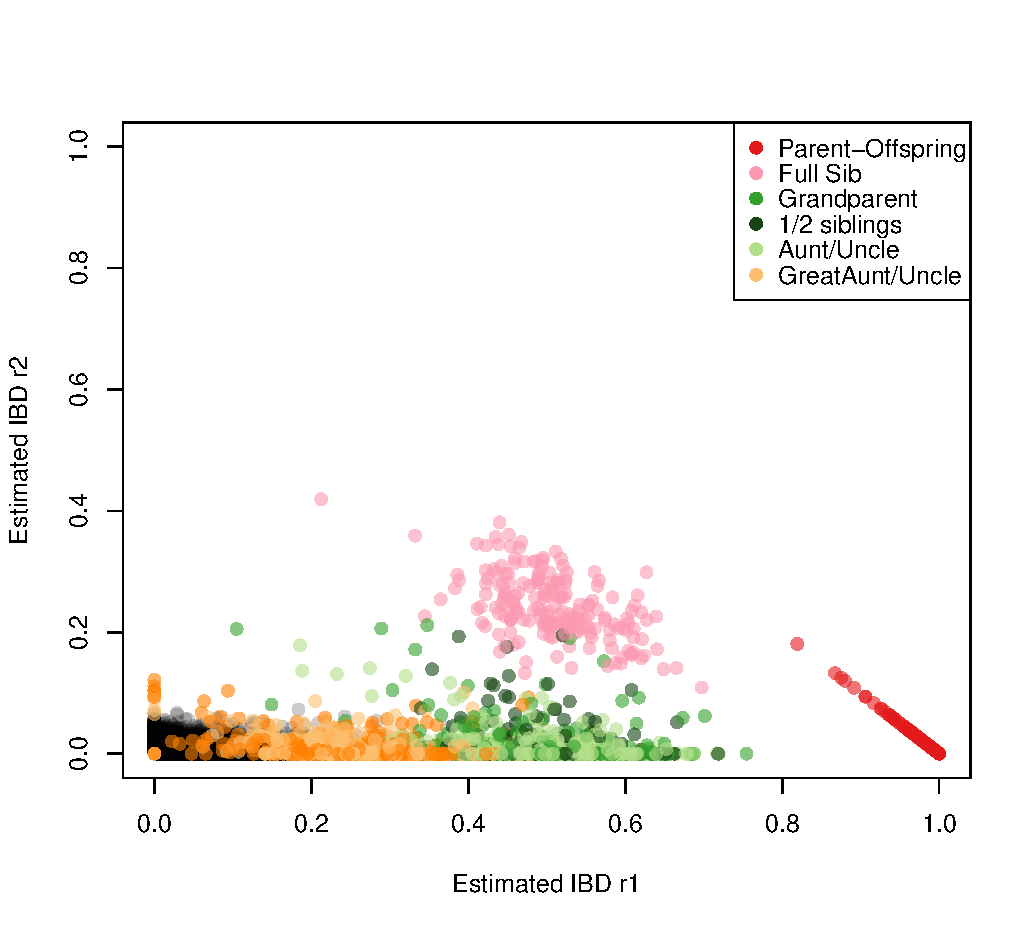
\includegraphics[width= 0.75 \textwidth]{figures/FSJ_IBD.pdf}
\end{center}
\caption[3cm]{Estimated coefficient
of kinship from Florida Scrub Jays. Each point is a pair of
individuals, plotted by their estimated IBD ($r_1$ and $r_2$) from their genetic data. The
points are coloured by their known pedigree relationships. Note that
most pairs have low kinship, and no recent genealogical relationship,
and so appear as black points in the lower left corner. Thanks to
Nancy Chen for supplying the data. \gitcode{https://github.com/cooplab/popgen-notes/blob/master/Rcode/FSJ_IBD/FSJ_IBD_plotting.R} } \label{fig:FSJ_IBD}
\end{figure}

\paragraph{Sharing of genomic blocks among relatives.}
\begin{figure}
\begin{center}
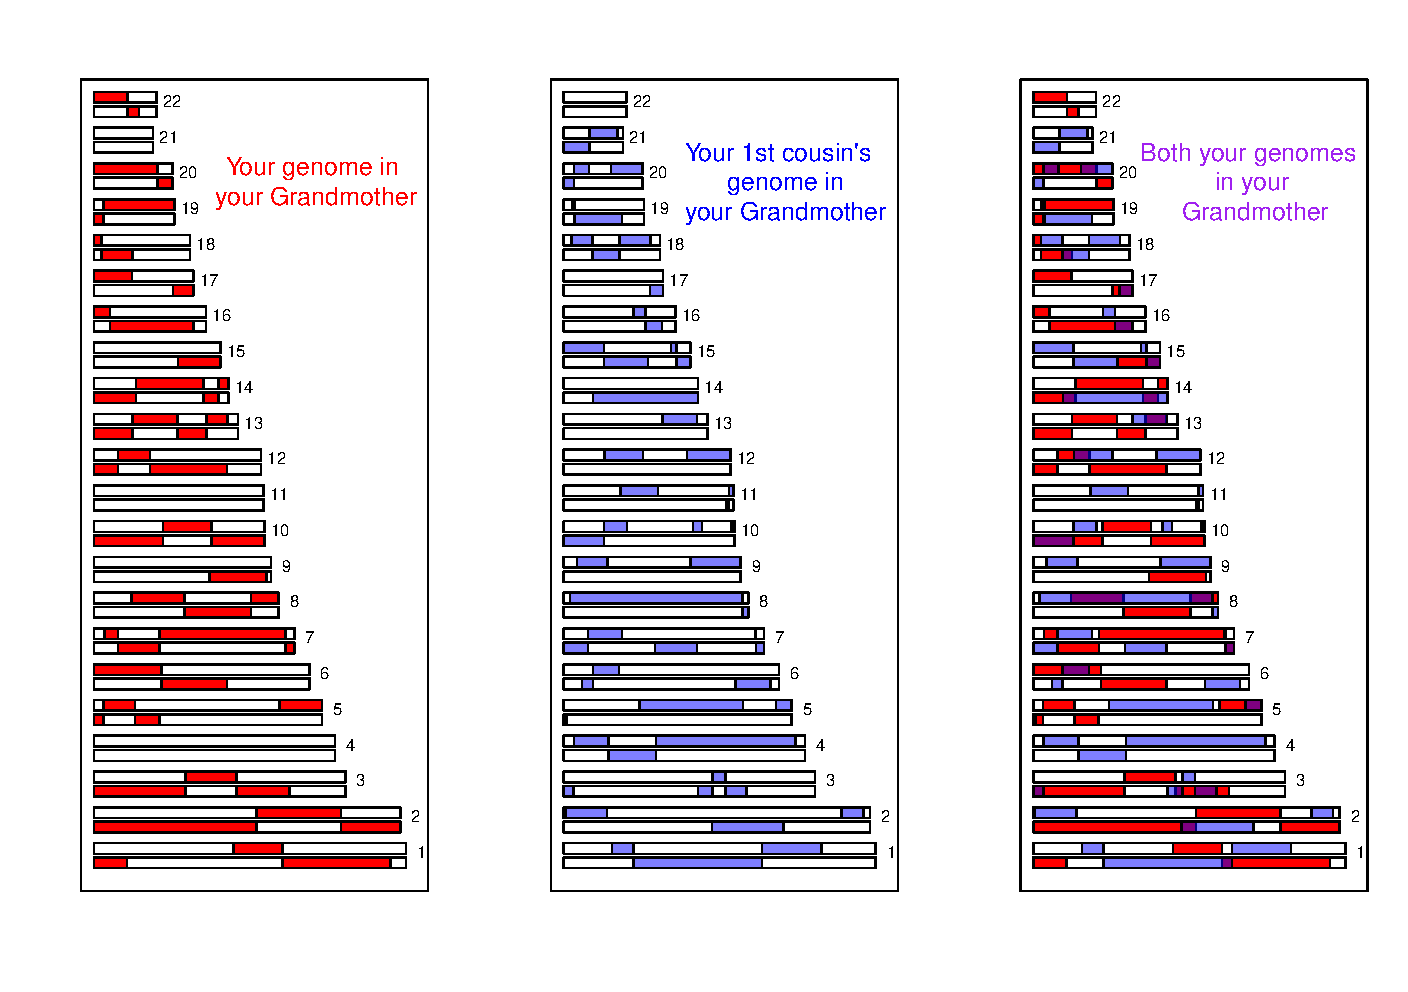
\includegraphics[width= \textwidth]{figures/sharing_relatives/First_cousin_overlap.pdf}
\end{center}
\caption[]{A simulation of sharing between first cousins. The regions of your grandmother's 22 autosomes that you inherited are
coloured red, those that your cousins inherited are coloured blue. In the third panel we show the overlapping genomic regions in purple, these regions will be IBD in you and your cousin. If you are full first cousins, you will also have shared genomic regions from your shared grandfather, not shown here. Details about how we made these simulations \href{https://gcbias.org/2013/12/02/how-many-genomic-blocks-do-you-share-with-a-cousin/}{here}.
} \label{fig:first_cousin_IBD}
\end{figure}
We can more directly see the sharing of the genome among close
relatives using high-density SNP genotyping arrays. In Figure \ref{fig:first_cousin_IBD} we show a simulation of you and your first cousin's genomic material that you both inherited from your shared grandmother. Colored purple are regions where you and your cousin will have matching genomic material, due to having inherited it IBD from your shared grandmother.
%JRI: text says ``Below'' but float ends up above



You and your first cousin will share at least one allele of your genotype at all of the polymorphic loci in these purple regions. There's a range of methods to detect such sharing. One way is to look for unusually long stretches of the genome where two individuals are never homozygous for different alleles. By identifying pairs of individuals who share an unusually large number of such putative IBD blocks, we can hope to identify unknown relatives in genotyping datasets. In fact, companies like 23\&me and Ancestry.com use signals of IBD to help identify family ties.

As another example, consider the case of third cousins. You share one of eight sets of great-great grandparents with each of your (likely many) third cousins. On average, you and each of your third cousins each inherit one-sixteenth of your genome from each of those two great-great grandparents. This turns out to imply that on average, a little less than one percent of your and your third cousin's genomes ($2 \times (1/16)^2 =0.78\%$) will be identical by virtue of descent from those shared ancestors. A simulated example where third cousins share blocks of their genome (on chromosome 16 and 2) due to their great, great grandmother is shown in Figure \ref{fig:third_cousin_IBD}.

\begin{figure}
\begin{center}
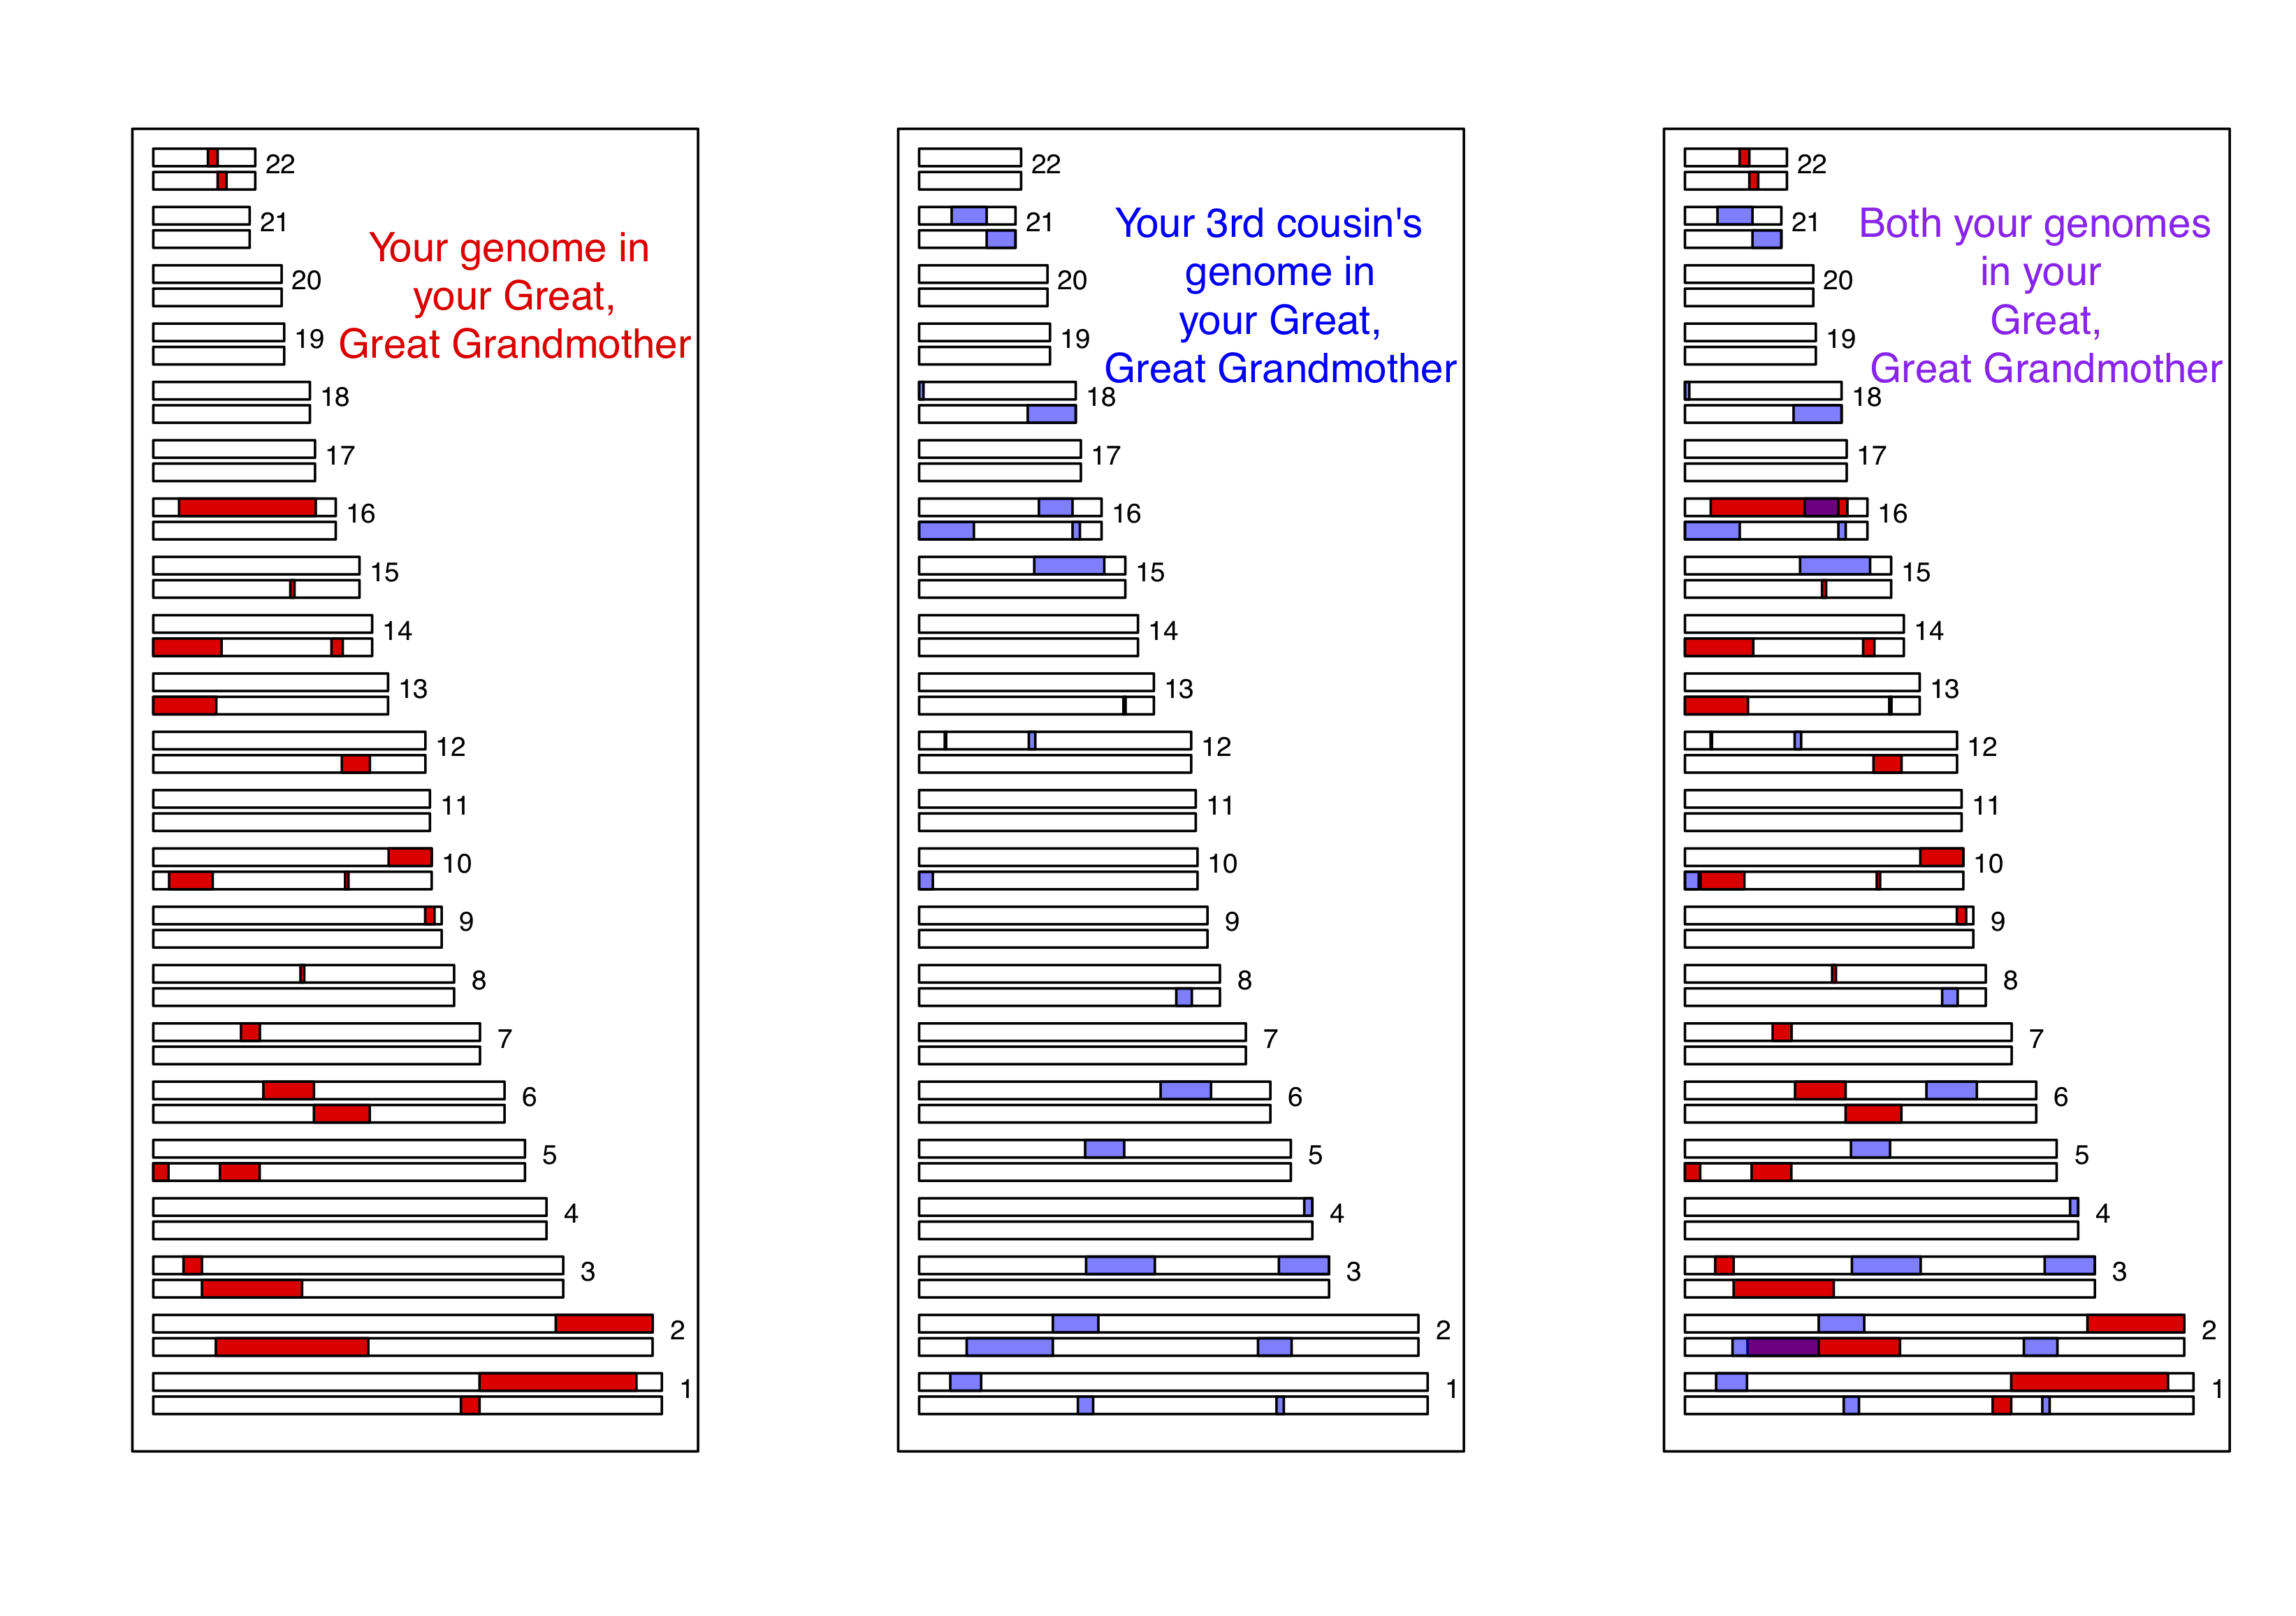
\includegraphics[width= \textwidth]{figures/sharing_relatives/Third_cousin_overlap_1.png}
\end{center}
\caption[]{A simulation of sharing between third cousins, the details are the same as in Figure \ref{fig:first_cousin_IBD}.} \label{fig:third_cousin_IBD}
\end{figure}


Note how if you compare Figure \ref{fig:third_cousin_IBD} and Figure \ref{fig:first_cousin_IBD}, individuals inherit less IBD from a shared great, great grandmother than from a shared grandmother, as they inherit from more total ancestors further back. Also notice how the sharing occurs in shorter genomic blocks, as it has passed through more generations of recombination during meiosis. These blocks are still detectable, and so third cousins can be detected using high-density genotyping chips, allowing more distant relatives to be identified than single marker methods alone. \sidenote{Indeed the suspect in case of the Golden State Killer was identified through identifying third cousins that genetically matched a DNA sample from an old crime scene (see a \href{https://gcbias.org/2018/05/07/how-lucky-was-the-genetic-investigation-in-the-golden-state-killer-case/}{here} for more details).} More distant relations than third cousins, e.g. fourth cousins, start to have a significant probability of sharing none of their genome IBD. But you have many fourth cousins, so you will share some of your genome IBD with some of them; however, it gets increasingly hard to identify the degree of relatedness from genetic data the deeper in the family tree this sharing goes.

\subsection{Inbreeding}
We can define an inbred individual as an individual whose parents are
more closely related to each other than two random individuals drawn
from some reference population.  \\


\begin{marginfigure}
\begin{center}
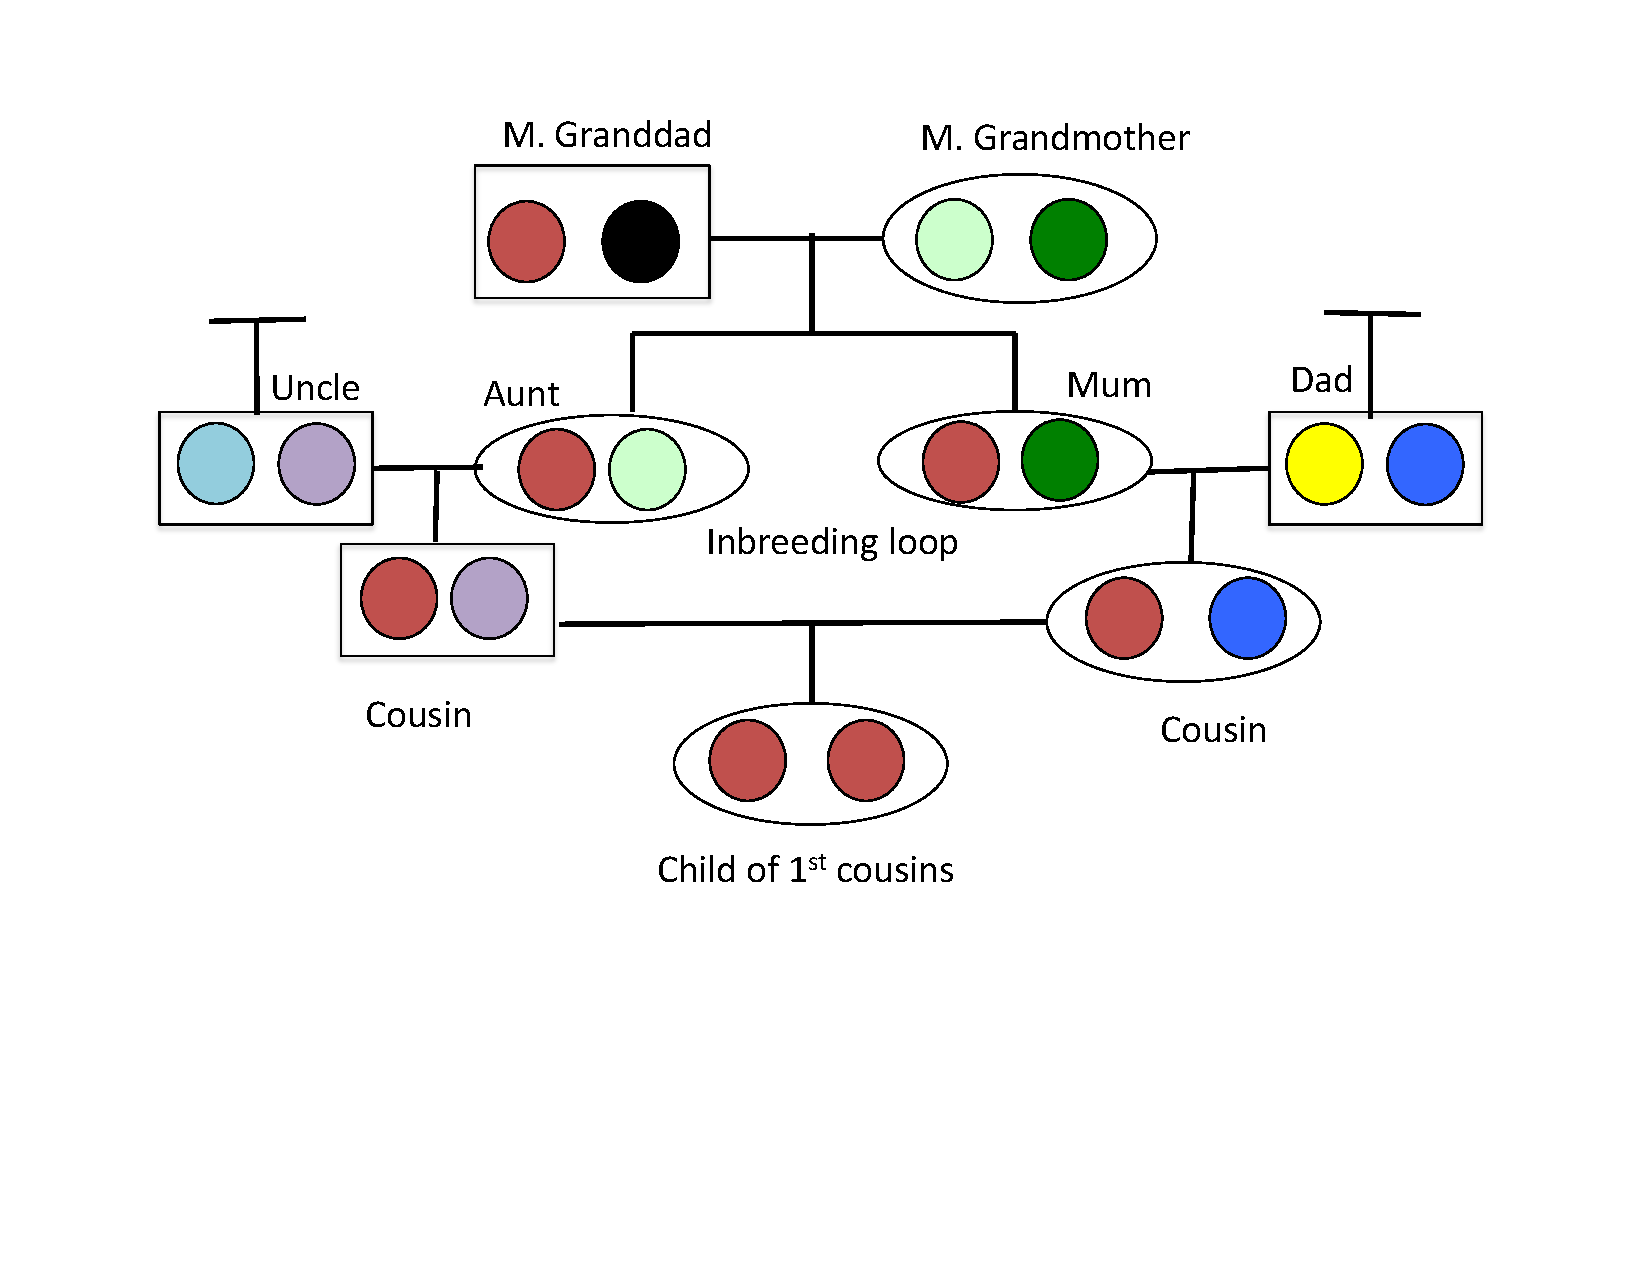
\includegraphics[width= \textwidth]{figures/Child_first_cousins_Homozy_BD.pdf}
\end{center}
\caption{Alleles being transmitted through an inbred pedigree. The two sisters (mum and aunt) share two alleles identical by descent (IBD). The cousins share one
  allele IBD. The offspring of first cousins is homozygous by
  descent at this locus.} \label{fig:IBD_cousins_cartoon}
\end{marginfigure}
\graham{Change this to have squares and circles}
When two related individuals produce an offspring, that individual can
receive two alleles that are identical by descent, i.e.\ they
can be homozygous by descent (sometimes termed autozygous), due to the
fact that they have two copies of an allele through different paths
through the pedigree.  This increased likelihood of being homozygous
relative to an outbred individual is the most obvious effect of
inbreeding. It is also the one that will be of most interest to us, as it
underlies a lot of our ideas about inbreeding depression and
population structure. For example, in Figure \ref{fig:IBD_cousins_cartoon} our
offspring of first cousins is homozygous by descent having received
the same IBD allele via two different routes around an inbreeding loop.\\

As the offspring receives a random allele from each parent ($i$ and $j$), the
probability that those two alleles are identical by descent is equal to the
kinship coefficient $F_{ij}$ of the two parents (Eqn.\ \ref{eqn:coeffkinship}). This follows from the fact that
the genotype of the offspring is made by sampling an allele at random from each
of our parents. % We will use IBD for identical by descent. \\ %% this was already defined above.

\begin{table}
\begin{center}
\begin{tabular}{ccc}
\hline
$f_{11}$ & $f_{12}$ & $f_{22}$ \\
\hline
$(1-F) p^2 + F p$ & $(1-F) 2pq$ & $(1-F) q^2 + F q$ \\
\hline
\end{tabular}
\end{center}
\caption{\textbf{Generalized Hardy--Weinberg}} \label{table:GeneralizedHWE}
\end{table}

The only way the offspring can be heterozygous ($A_1 A_2$) is if their two
alleles at a locus are not IBD (otherwise they would necessarily be
homozygous). Therefore, the probability that they are heterozygous is

\begin{equation}
(1-F) 2p q,
\label{eq:hetGenHW}
\end{equation}
%
where we have dropped the indices $i$ and $j$ for simplicity.  The offspring
can be homozygous for the $A_1$ allele in two different ways.  They can have
two non-IBD alleles that are not IBD but happen to be of the allelic type
$A_1$, or their two alleles can be IBD, such that they inherited allele $A_1$
by two different routes from the same ancestor. Thus, the probability that an
offspring is homozygous for $A_1$ is

\begin{equation}
(1-F) p^2 + F p.
\end{equation}
%
Therefore, the frequencies of the three possible genotypes can be written as given in
Table \ref{table:GeneralizedHWE}, which provides a generalization of the Hardy--Weinberg
proportions.\\


%Note that the generalized Hardy--Weinberg proportions completely
%specify the genotype probabilities, as there are two parameters ($p$ and $F$)
%and two degrees of freedom (as $p$ and $q$ have to sum to one).
%Therefore, any combination of genotype frequencies at a biallelic site
%can be specified by a combination of $p$ and $F$.\\
%JRI: unclear to me if this is useful. will readers understand parameter numbers/DF?

\begin{question}
The frequency of the $A_1$ allele is $p$ at a biallelic locus. Assume that our population is randomly mating and that the
genotype frequencies in the population follow from HW. We select two
individuals at random to mate from this population. We then mate the children
from this cross. What is the probability that the child from this full
sib-mating is
homozygous?
\end{question}

\paragraph{Multiple inbreeding loops in a pedigree.}
Up to this point we have assumed that there is at most one inbreeding loop in the recent family history of our
  individuals, i.e. the parents of our inbred individual have at most one recent genealogical connection. However, an individual who has multiple inbreeding loops in their pedigree can be homozygous by
  descent thanks to receiving IBD alleles via multiple different different loops. To calculate inbreeding in pedigrees of arbitrary complexity, we can extend
 beyond our original relatedness coefficients $r_0$, $r_1$, and $r_2$ to account for
 higher order sharing of alleles IBD among relatives. For example,
 we can ask, what is the probability that \textit{both} of the alleles in the first individual
 are shared IBD with one allele in the second individual? There are
 nine possible relatedness coefficients in total to completely describe kinship between two diploid individuals, and we won't go in to them here
 as it's a lot to keep track of.
However, we will show how we can calculate the inbreeding coefficient of an
individual with multiple inbreeding loops more directly.\\

%ut at loci where the ancestor is inbred you get two more options (C inherits maternal/B paternal or opp.) so the factor of 2 applies to fA as well and cancels out for both.}

Let's say the parents of our inbred individual (B and C) have $K$ shared ancestors,
i.e. individuals who appear in both B and C's recent family trees. We denote these shared ancestors by $A_1, \dots,A_K$, and we denote by $n$ the total number of individuals in the chain from B to C via ancestor $A_i$, including B, C, and $A_i$. For example, if B is C's aunt, then B and C share two ancestors, which are B's parents and, equivalently, C's grandparents. In this case, there are n=4 individuals from B to C through each of these two shared ancestor. In the general case, the kinship coefficient of B and C,
i.e. the inbreeding coefficient of their child, is
\begin{equation}
 F = \sum_{i=1}^K \frac{1}{2^{n_i}} \big( 1+ f_{A_i} \big)
\end{equation}
where $f_{A_i}$ is the inbreeding coefficient of the ancestor
$A_i$. What's happening here is that we sum over all the mutually-exclusive paths in the pedigree through which B and C can share an allele IBD. With probability
$\nicefrac{1}{2^{n_i}}$, a pair of alleles picked at random from B and C is descended from the same ancestral allele in individual
$A_i$, in which case the alleles are IBD. \sidenote{For example, in the case of our aunt-nephew case, assuming that the aunt's two parents are their only recent shared ancestors, then $F = \nicefrac{1}{2^4}+\nicefrac{1}{2^4} = \nicefrac{1}{8}$, in agreement with the answer we would obtain from  eqn \eqref{eqn:coeffkinship}.} However, even if B inherits the maternal allele and C inherits the paternal allele of shared ancestor $A_i$, if $A_i$ was
themselves inbred,  with probability $f_{A_i}$ those two
alleles are themselves IBD. Thus a shared \textit{inbred} ancestor further increases
the kinship of B and C.

\begin{figure}
  \begin{center}
  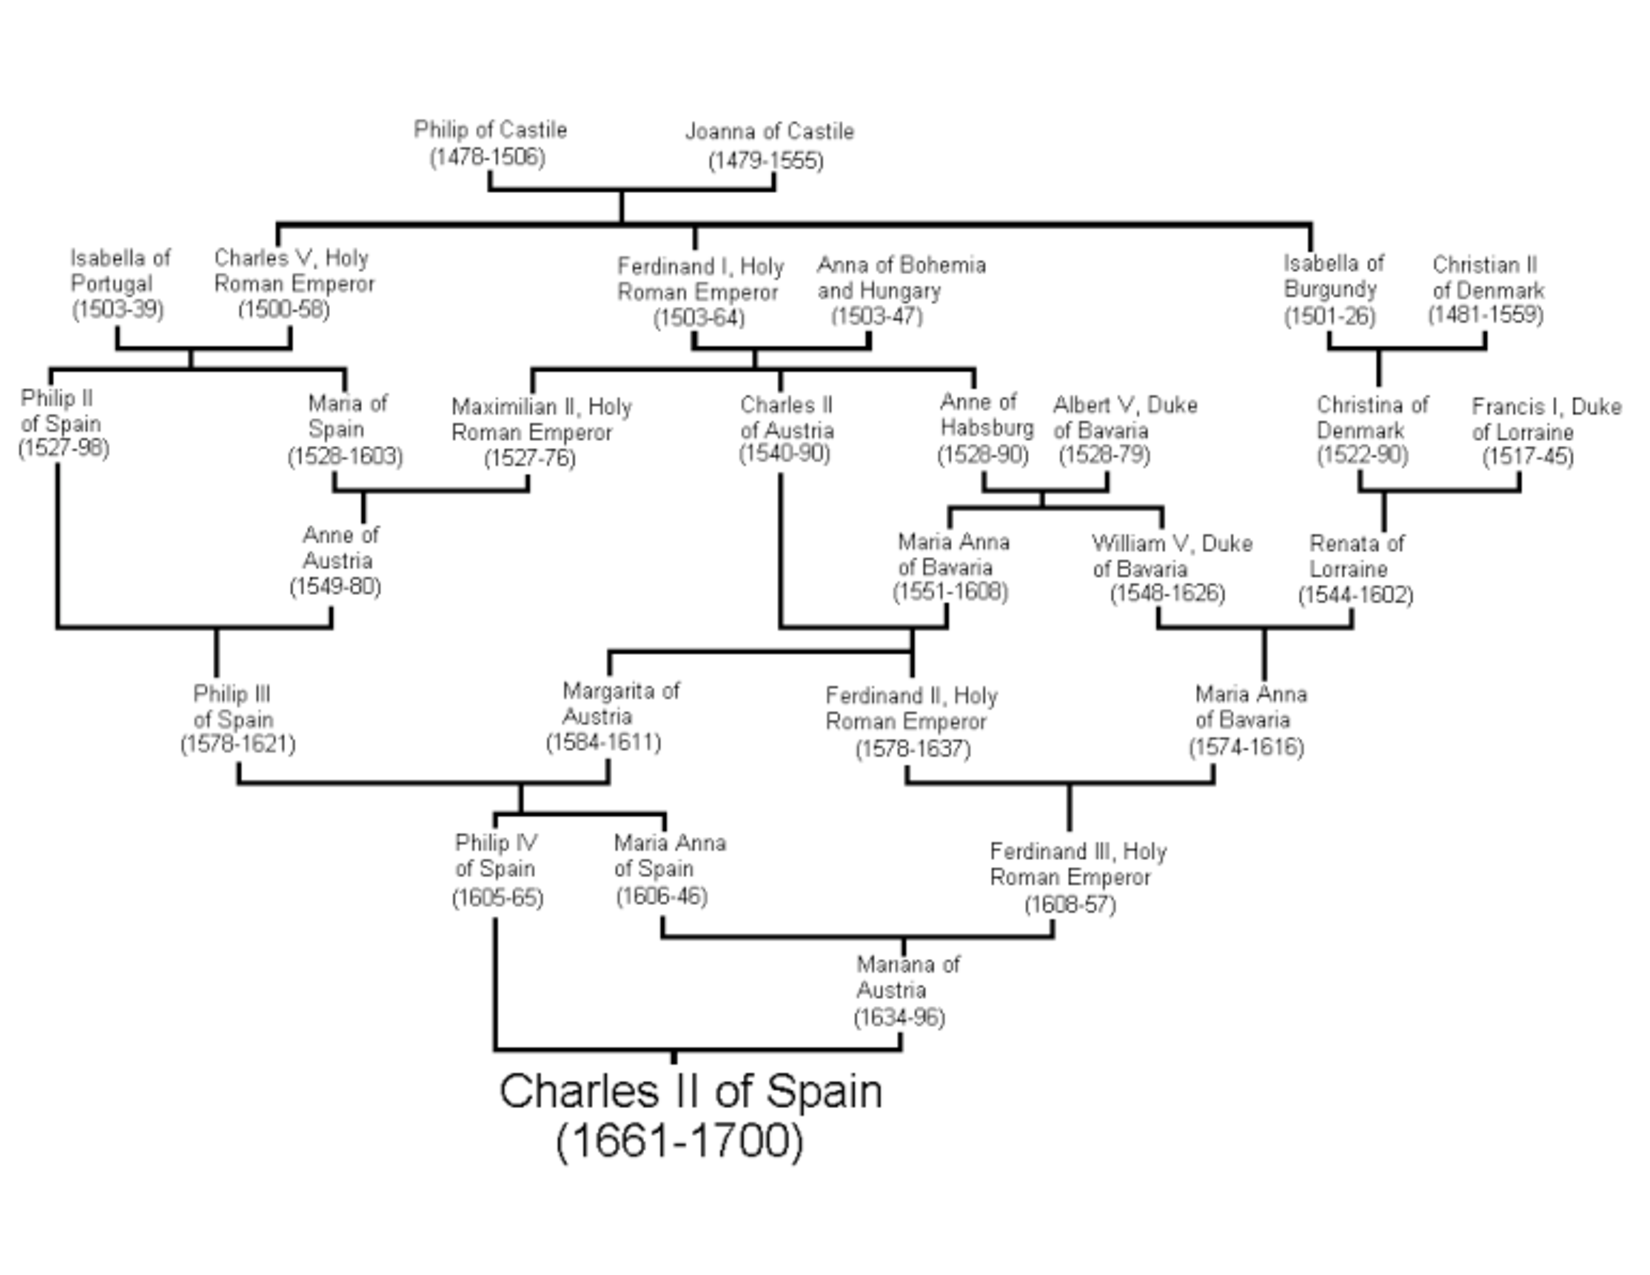
\includegraphics[width=
  \textwidth]{Journal_figs/alleles_genotypes/Charles_second_pedigree/Carlos_second_pedigree_2_trimmed.pdf}  %https://commons.wikimedia.org/wiki/File:Carlos_segundo80.png
\end{center}
\caption{The pedigree of King Charles II of
  Spain. Pedigree from
  \href{https://commons.wikimedia.org/wiki/File:Carlos_segundo80.png}{wikimedia}
drawn by \href{https://en.wikipedia.org/wiki/User:Lec_CRP1}{Lec CRP1},
public domain.} \label{fig:Carlos_second_pedigree}
\end{figure}
\begin{marginfigure}
\begin{center}
  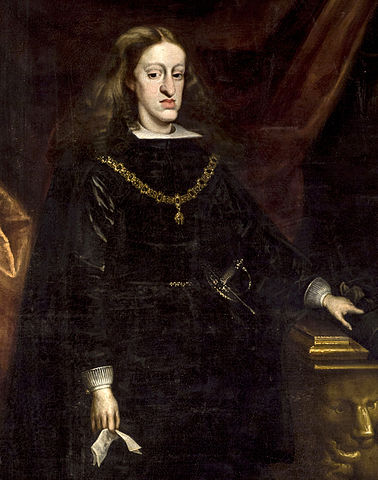
\includegraphics[width=
  \textwidth]{illustration_images/alleles_genotypes/Carlos_second/378px-Juan_de_Miranda_Carreno_002.jpg}
%https://commons.wikimedia.org/wiki/File:Carlos_segundo80.png
\end{center}
\caption{Charles II of Spain (by Juan Carre\~{n}o de Miranda,
  1685). \href{https://it.wikipedia.org/wiki/Carlo_II_di_Spagna\#/media/File:Juan_de_Miranda_Carreno_002.jpg}{Public Domain}.} \label{fig:Carlos_second}
\end{marginfigure}
Multiple inbreeding loops increase the probability that a child
is homozygous by descent at a locus, which can be calculated simply by plugging in $F$, the child's
inbreeding coefficient, into our generalized HW equation.


As one extreme example of the impact of multiple inbreeding loops in
an individual's pedigree, let's consider king Charles II of
Spain, the last of the Spanish Habsburgs.  Charles was the son of
Philip IV of Spain and Mariana of Austria, who were uncle and
niece. If this were the only inbreeding loop, then Charles would have had an
inbreeding coefficient of $\nicefrac{1}{8}$. Unfortunately for Charles, the
Spanish Habsburgs had long kept wealth and power within their family
by arranging marriages between close kin. The pedigree of Charles II is shown in Figure \ref{fig:Carlos_second_pedigree}, and
multiple inbreeding loops are apparent. For example, Phillip III,
Charles II's grandfather and great-grandfather, was himself a child of
an uncle-niece marriage.

\citet{alvarez:09} calculated that Charles II had an inbreeding
coefficient of $0.254$, equivalent to a full-sib mating,
thanks to all of the inbreeding loops in his pedigree. Therefore, he
is expected to have been homozygous by descent for a full quarter of his
genome. As we'll talk about later in these notes, this means that Charles
may have been homozygous for a number of recessive disease alleles,
and indeed he was a very sickly man who left no descendants due to his
infertility. \sidenote{Pedro Gargantilla, who performed Charles's autopsy, stated
  that his body ``did not contain a single drop of blood; his heart was
  the size of a peppercorn; his lungs corroded; his intestines rotten
  and gangrenous; he had a single testicle, black as coal, and his
  head was full of water.'' While some of this description
  may refer to actual medical conditions, some of these details seem a
  little unlikely. See
  \href{https://www.thevintagenews.com/2017/03/23/when-charles-ii-of-spain-died-the-autopsy-stated-that-his-body-did-not-contain-a-single-drop-of-blood-and-his-head-was-full-of-water/}{here}.
} Thus plausibly the end of one of the great
European dynasties came about through inbreeding. 
%JRI: good idea to include links to potentially impermanent websites?


\subsection{Calculating inbreeding coefficients from genetic data}

%JRI: you transition from an individual's inbreeding coefficient here to using F as a population inbreeding parameter. i think some text explaining this change of scope might help

If the observed heterozygosity in a population is $H_O$, and we assume that the
generalized Hardy--Weinberg proportions hold, we can set $H_O$ equal to
$f_{12}$, and solve Eq.\ \eqref{eq:hetGenHW} for $F$ to obtain an estimate of
the inbreeding coefficient as

\begin{equation}
\hat{F} = 1-\frac{f_{12}}{2pq} = \frac{2pq - f_{12}}{2pq}.
\label{eqn:Fhat}
\end{equation}

As before, $p$ is the frequency of allele $A_{1}$ in the population. This can
be rewritten in terms of the observed heterozygosity ($H_O$) and the
heterozygosity expected in the absence of inbreeding, $H_E=2pq$, as
\begin{equation}
\hat{F} = \frac{H_E-H_O}{H_E} = 1 - \frac{H_O}{H_E}.
\label{eqn:FhatHO}
\end{equation}
Hence, $\hat{F}$ quantifies the deviation due to inbreeding of the observed heterozygosity from the one expected under random mating, relative to the latter.

\begin{question}
  Suppose the following genotype frequencies were observed for an esterase locus in a population of \textit{Drosophila} (A denotes the ``fast" allele and B denotes the ``slow" allele):
\begin{center}
\begin{tabular}{ccc}
\hline
AA &	AB &	BB\\
\hline
0.6 &	0.2 &	0.2\\
\end{tabular}
\end{center}
What is the estimate of the inbreeding coefficient at the esterase locus?
\end{question}

If we have multiple loci, we can replace $H_O$ and $H_E$ by their means
over loci, $\bar{H}_O$ and $\bar{H}_E$, respectively. Note that, in principle, we could also calculate $F$ for each individual locus first, and then take the average across loci. However, this procedure is more prone to introducing a bias if sample sizes vary across loci, which is not unlikely when we are dealing with real data.


Genetic markers are commonly used to estimate inbreeding for wild and/or captive populations of conservation concern. As an example of this, consider the case of the Mexican wolf ({\it Canis lupus baileyi}), a sub-species of gray wolf. \begin{marginfigure}[-2cm]
\begin{center}
  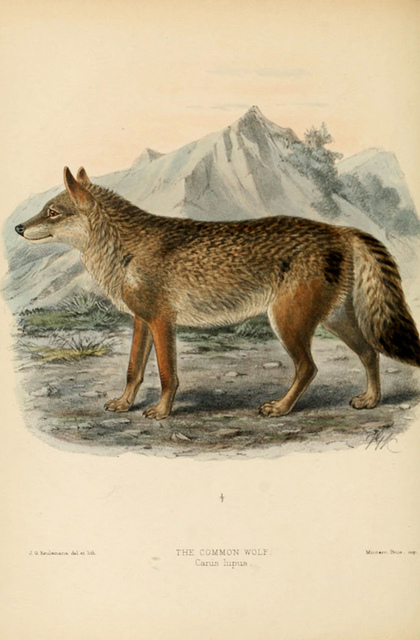
\includegraphics[width= \textwidth]{illustration_images/alleles_genotypes/grey_wolf/5988399184_0c36a8e51c_z.jpg}
\end{center}
\caption{Grey wolf ({\it Canis lupus}). \BHLNC{Dogs, jackals, wolves,
    and foxes: a monograph of the Canidae. 1890. y J.G. Keulemans}{https://www.biodiversitylibrary.org/page/17002968\#page/58/mode/1up}{University of Toronto - Gerstein Science Information Centre}} \label{fig:Grey_wolf}
\end{marginfigure}
They were extirpated in the wild during the mid-1900s due to hunting, and the remaining five Mexican wolves in the wild were captured to start a breeding program. \citet{vonHoldt:11} estimated the current-day, average expected heterozygosity to be $0.18$, based on allele frequencies at over forty thousand SNPs. However, the average Mexican wolf individual was only observed to be heterozygous at $12\%$ of these SNPs. Therefore, the average inbreeding coefficient for the Mexican wolf is $F = 1 -\nicefrac{0.12}{0.18}$, i.e. $\sim 33 \%$ of a lobo's genome is homozygous due to recent inbreeding in their pedigree.

%{\bf Q}\arabic{Question} \refstepcounter{Question}

%==Phenotypic resemblance between relatives ==
%<source-file filename="Quantative_traits.tex" display="Quantative_traits.wrapped.latexml.xhtml">

%==Phenotypic resemblance between relatives ==
%<source-file filename="Quantative_traits.tex" display="Quantative_traits.wrapped.latexml.xhtml">

  \paragraph{Genomic blocks of homozygosity due to inbreeding.}

As we saw above, close relatives are expected to share alleles IBD in
large genomic blocks. Thus, when related individuals mate and transmit
alleles to an inbred offspring, they transmit these alleles in big
blocks through meiosis. An example, lets return to the case of our
hypothetical first cousins from Figure
\ref{fig:IBD_cousins_chr_cartoon}. If this pair of individuals had a
child, one possible pattern of genetic transmission is shown in Figure
\ref{fig:kid_first_cousins}. The child has inherited the red stretch
of chromosome via two different routes through their predigree from
the grandparents. This is an example of an autozygous
segment, where the child is homozygous by descent at all of the loci in this
red region.
  \begin{figure}
  \begin{center}
    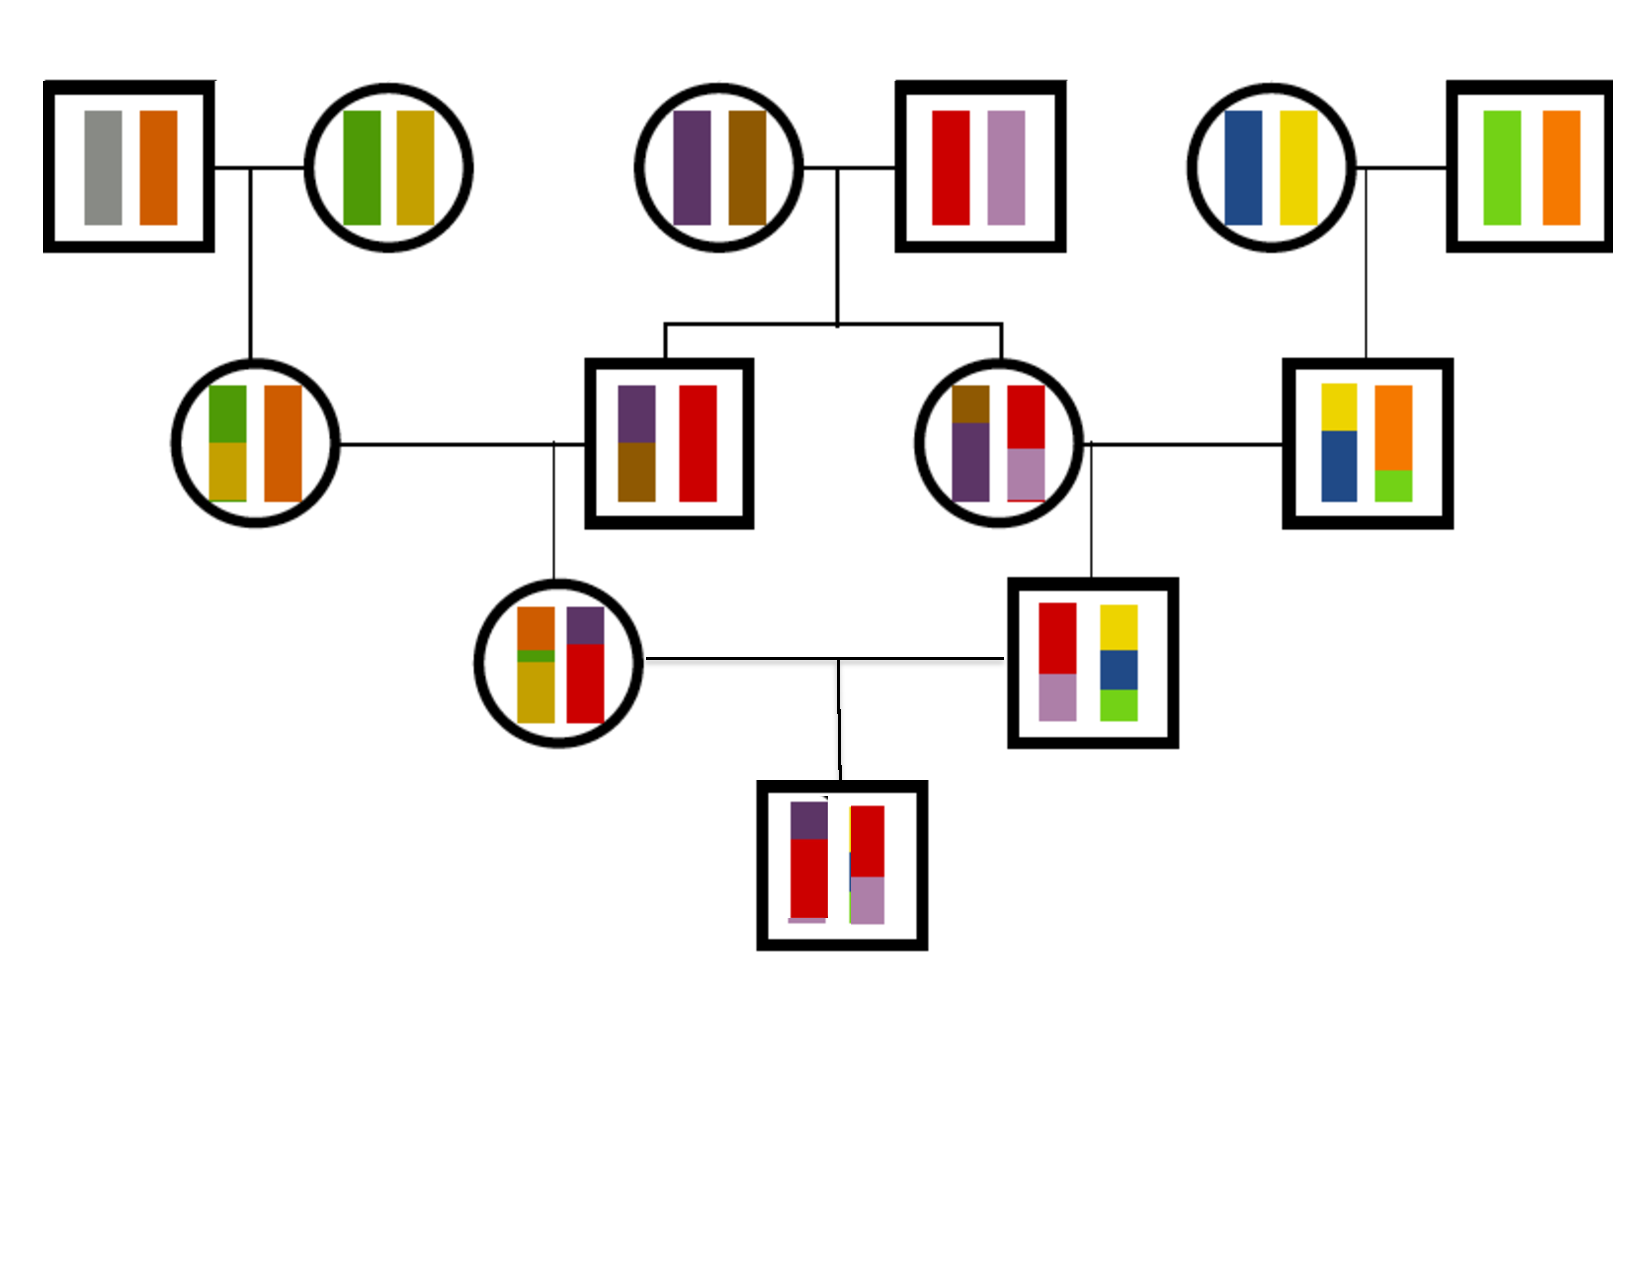
\includegraphics[width= 0.75 \textwidth]{figures/sharing_relatives/first_cousin_offspring.pdf}
\end{center}
\caption{A pedigree showing the offspring of first cousins. The
  chromosomes of their great-grandparents are coloured different colours
so their transmission can be tracked. The child is homozygous by
descent (HBD) for a section of the red chromosome.} \label{fig:kid_first_cousins}
\end{figure}
The inbreeding coefficient of the child sets the proportion of their
genome that will be in these autozygous segments. For example, a child
of first full cousins is expected to have $1/16$ of their
genome in these segments.
The more distant the loop in the pedigree, the more meioses that
chromosomes have been through and the shorter individual blocks will be. A
child of first cousins will have longer blocks than a child of second
cousins, for example.

Individuals with multiple inbreeding loops in their family tree can
have a high inbreeding coefficient due to
the combined effect of many small blocks of autozygosity. For example, Charles II had
an inbreeding coefficient that is equivalent to that of the child of
full-sibs, with a quarter of his genome expected to homozygous by
descent, but this would be made up of many shorter blocks.
%With multiple rounds of inbreeding individuals can

We can hope to detect these blocks by looking for unusually long
genomic runs of homozygosity (ROH) sites in an individual's genome. One way to
estimate an individual's inbreeding coefficient is then to total up
the proportion of an individual's genome that falls in such ROH
regions. This estimate is called $F_{ROH}$.

\graham{update to use figs from G3 Sam's article, and collapse to
  single ref.}
An example of using $F_{ROH}$ to study inbreeding comes from the work of
\citet{sams2018fine}, who identified runs of homozygosity in 2,500 dogs,
ranging from 500kb up to many megabases.
  \begin{figure}
  \begin{center}
    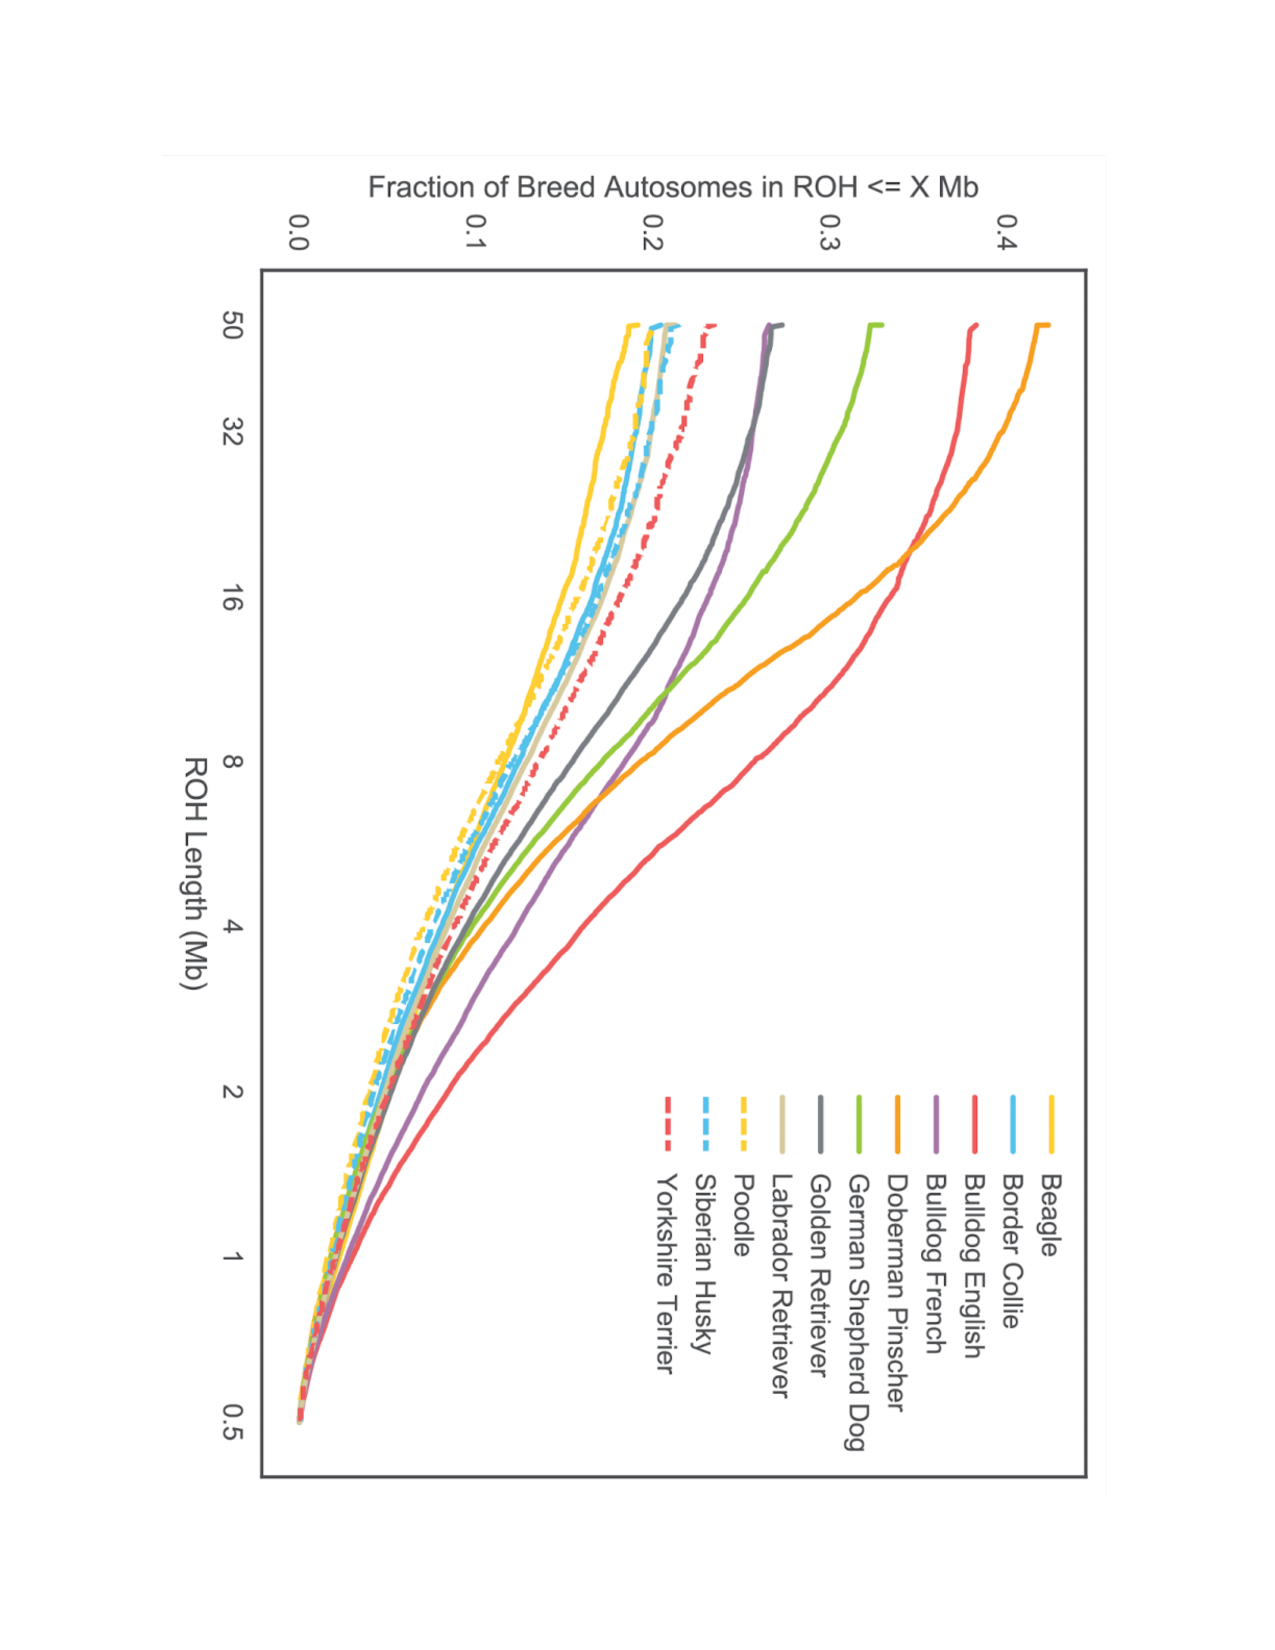
\includegraphics[width= \textwidth]{figures/sharing_relatives/dogs_FROH.pdf}
\end{center}
\caption{The distribution  of $F_{ROH}$ of individuals from various
  dog breeds from \citet{Sams:18}, \PLOSccBY.} \label{fig:dog_FOH}
\end{figure}
Figure
\ref{fig:dog_FOH} shows the distribution of $F_{ROH}$ of individuals in each dog
breed for the X and autosome. In Figure \ref{fig:dog_FOH_dist} this is
broken down by the length of ROH segments.
%JRI: No text reference to this figure. Why show a bulldog and not a mix of dog breeds?

  \begin{marginfigure}[-1cm]
  \begin{center}
    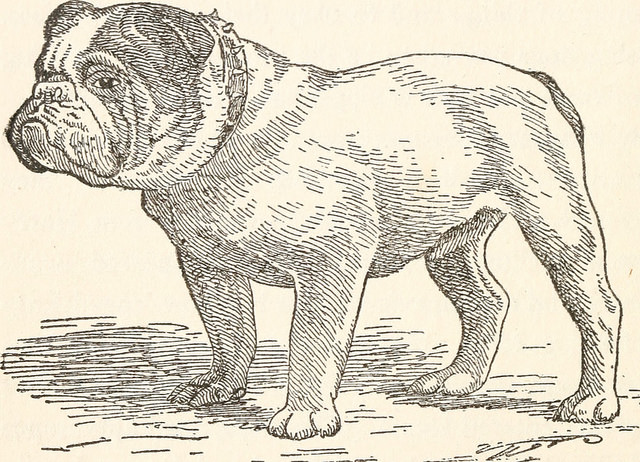
\includegraphics[width=
    \textwidth]{illustration_images/alleles_genotypes/english_bulldog/14752595581_4330377c97_z.jpg}
\end{center}
\caption{English bulldog. The dogs of Boytown. 1918.  Dyer, W. A.} \label{fig:bulldog}
\end{marginfigure}

Dog breeds have been subject
to intense breeding that has resulted in high levels of inbreeding. Of the population samples examined, Doberman Pinschers have the highest levels of their genome in runs of
homozygosity ($F_{ROH}$), somewhat higher than English bulldogs. In \ref{fig:dog_FOH_dist} we can see that English bulldogs have more short ROH than Doberman Pinschers, but that Doberman Pinschers have more of their genome in very large ROH ($>16 Mb$). This suggests that English bulldogs have had long history of inbreeding but that Doberman Pinschers have a lot of recent inbreeding in their history.

  \begin{figure}
  \begin{center}
    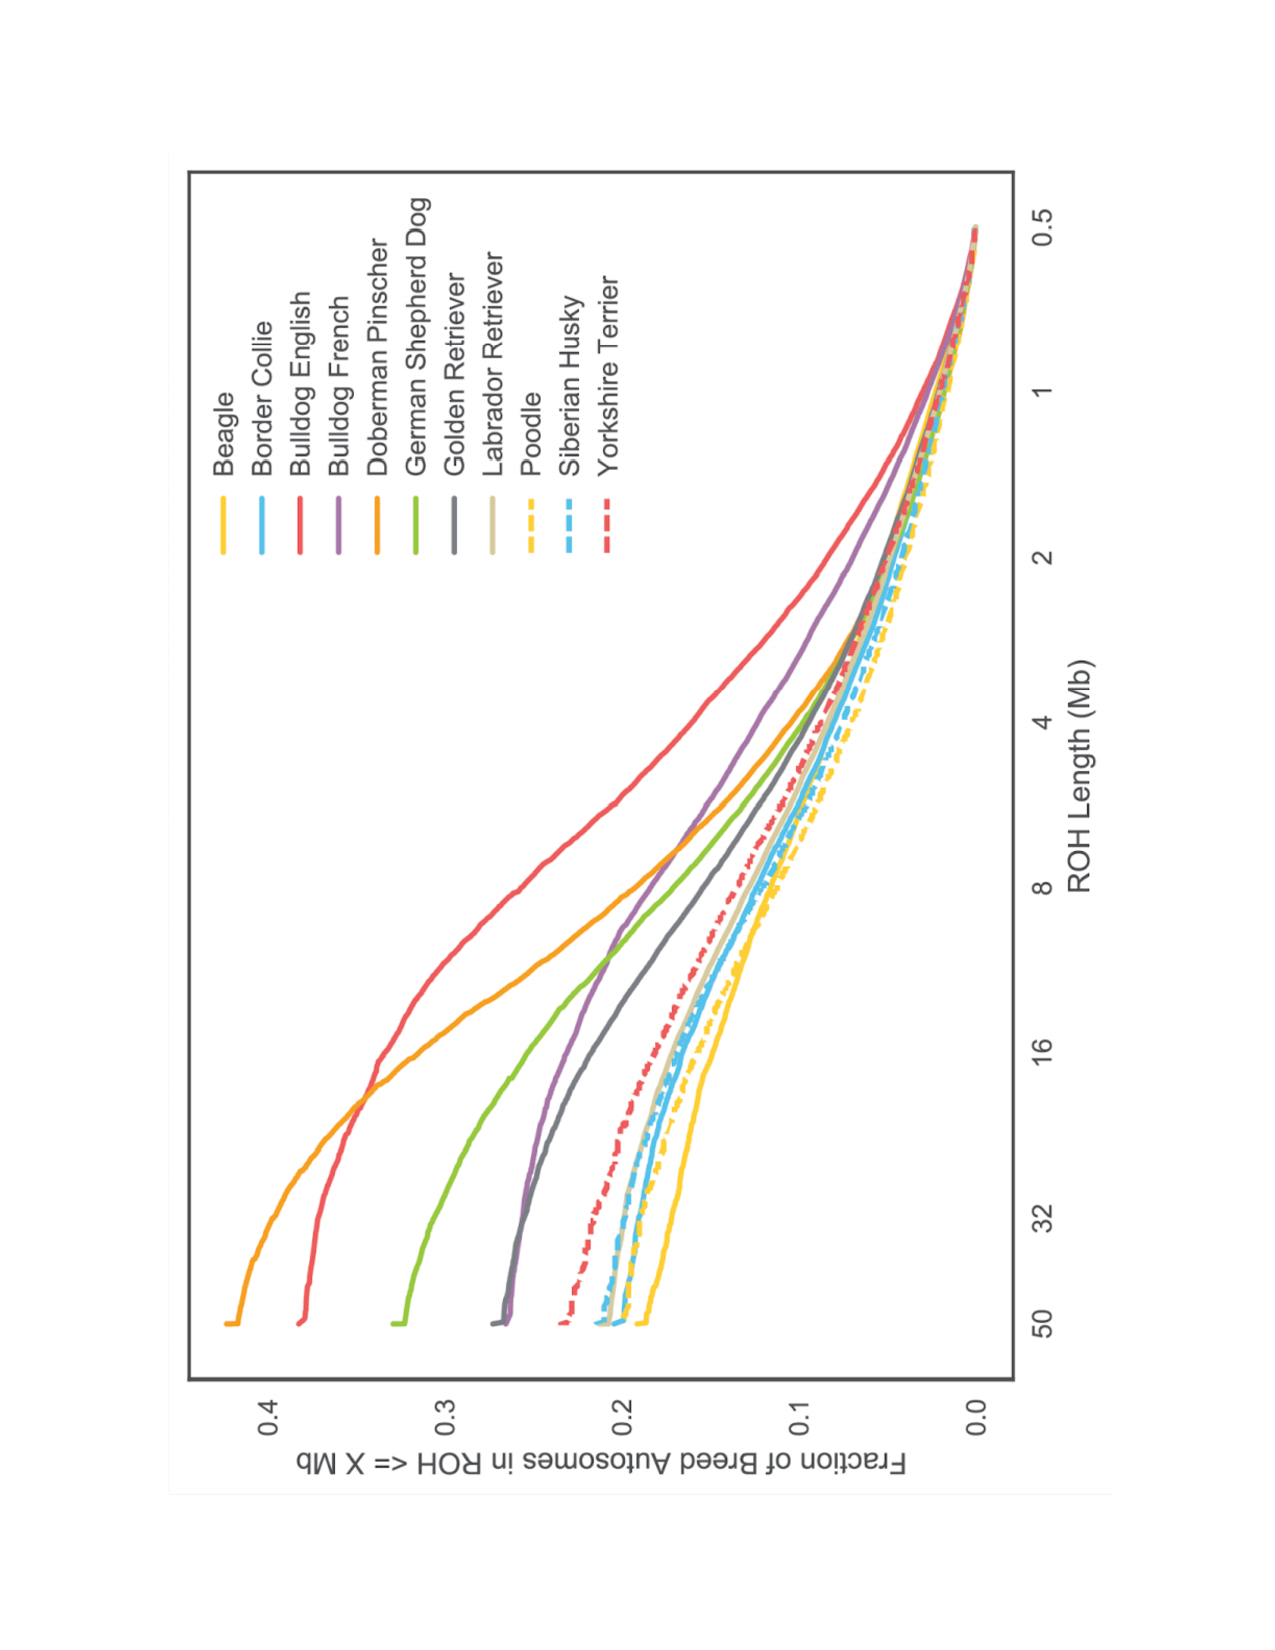
\includegraphics[width= \textwidth]{figures/sharing_relatives/dog_FROH_dist.pdf}
\end{center}
\caption{Cumulative density of ROH length, measured in megabases (Mb) from \citet{Sams:18} for various
  dog breeds (\PLOSccBY). Note that longer lengths of ROH are on the left of the plot.} \label{fig:dog_FOH_dist}
\end{figure}

\chapter{Genetic Drift and Neutral Diversity}

\newthought{Randomness is inherent to evolution}, from the lucky birds blown of course to colonize some new oceanic island, to which mutations arise first in the HIV strain infecting an individual taking anti-retroviral drugs. One major source of stochasticity in evolutionary biology is genetic drift.  Genetic drift occurs because more or less copies of an allele by chance can be transmitted to the next generation. This can occur because, by chance, the individuals carrying a particular allele can leave more or less offspring in the next generation. In a
sexual population, genetic drift also occurs because Mendelian transmission
means that only one of the two alleles in an individual, chosen at random at a
locus, is transmitted to the offspring. 

Genetic drift can play a role in the dynamics of all alleles in all populations, but it will play the biggest role for neutral alleles. A neutral polymorphism occurs when the segregating alleles at a polymorphic site have no discernible differences in their effect on fitness. We'll make clear what we mean by "discernible" later, but for
the moment think of this as "no effect" on fitness. 
\paragraph{The neutral theory of molecular evolution.} 
The role of genetic drift in molecular evolution has been hotly debated since the 60s when he Neutral theory of molecular evolution was proposed \citep[see ][ for a history]{ohta1996development}.\cite{kimura:68,king:69,kimura:83}.  The central premise of Neutral theory theory is that patterns of molecular polymorphism within species and substitution between species can be well understood by supposing that the vast majority of these molecular polymorphisms and substitutions were neutral alleles, whose dynamics were just subject to the vagaries of genetic drift and mutation. Early proponents of this view suggested that the vast majority of new mutations are either neutral or highly deleterious (e.g. mutations that disrupt important protein functions). This latter class of mutations are too deleterious to contribute much to common polymorphisms or substitutions between species, because they are quickly weeded out of the population by selection. 

Neutral theory can sound strange given that much of the time our first brush with evolution often focuses of adaptation and phenotypic evolution. However, proponents of this world-view didn't deny the existence of advantageous mutations, they simply thought that beneficial mutations are rare enough that their contribution to the bulk of polymorphism or divergence can be largely ignored. They also often thought that much of phenotypic evolution may well be adaptive, but again the loci responsible for these phenotypes are a small fraction of all the molecular change that occur. The original neutral theory of molecular evolution was original proposed to explain protein polymorphism. However, we can apply it more broadly to think about neutral evolution genome-wide. With that in mind, what types of molecular changes could be neutral? Perhaps:
\begin{enumerate}
\item Changes in non-coding DNA that don't disrupt regulatory sequences. For example, in the human genome only about 2\% of the genome codes for proteins. The rest is mostly made up of old transposable element and retrovirus insertions, repeats, pseudo-genes, and general genomic clutter. Current estimates suggesting that, even counting conserved, functional, non-coding regions that $<10\%$ of our genome is subject to evolutionary constraint \citep{rands:14}.   
\item Synonymous changes in coding regions, i.e. those that don't change the amino-acid encoded by a codon.
\item Non-synonymous changes that don't have a strong effect on the functional properties of the amino acid encoded, e.g. changes that don't change the size, charge, or hydrophobic properties of the amino acid too much.
\item An amino-acid change with phenotypic consequences, but little relevance to fitness, e.g. a mutation that causes your ears to be a slightly different shape, or that prevents an organism from living past 50 in a species where most individuals reproduce and die by their 20s.
\end{enumerate}
There are counter examples to all of these ideas, e.g. synonymous changes can affect the translation speed and accuracy of proteins and so are subject to selection. However, the list above hopefully convinces you that the general thinking that some portion of molecular change may not be subject to selection isn't as daft as it may have initially sounded. 

Various features of molecular polymorphism and divergence have been viewed as consistent with the neutral theory of molecular evolution. The two we'll focus on in this chapter are the high level of molecular polymorphism in many species, see for example Figure \ref{fig:Leffer}, and the molecular clock. We'll see that various aspects of the original neutral theory have merit in describing some features and types of molecular change, but we'll also see that it is demonstrably wrong in some cases. We'll also see the primary utility of the neutral theory isn't whether it is right or wrong, but that it serves as a simple null model that can be tested and in some cases rejected, and subsequently built on. The broader debate currently in the field of molecular evolution is the balance of neutral, adaptive, and deleterious changes that drive different types of evolutionary change.  

\section{Loss of heterozygosity due to drift.} \label{LossofHet} 

Genetic drift will, in the absence of new mutations, slowly purge our population of neutral genetic diversity, as alleles slowly drift to high or low
frequencies and are lost or fixed over time. \\

Imagine a randomly mating population of a constant size $N$ diploid individuals, and that we
are examining a locus segregating for two alleles that are neutral with respect
to each other.  This population is randomly mating with respect to the alleles
at this locus. See Figures \ref{fig:LossHet_two_alleles} and
\ref{fig:LossHet_many_alleles} to see how genetic drift proceeds, by tracking
alleles within a small population. \\


In generation $t$ our current level of heterozygosity is $H_t$,
i.e. the probability that two randomly sampled alleles in generation
$t$ are non-identical is $H_t$. Assuming that the mutation rate is
zero (or vanishing small), what is our level of heterozygosity in
generation $t+1$?\\

\begin{figure}
\begin{center}
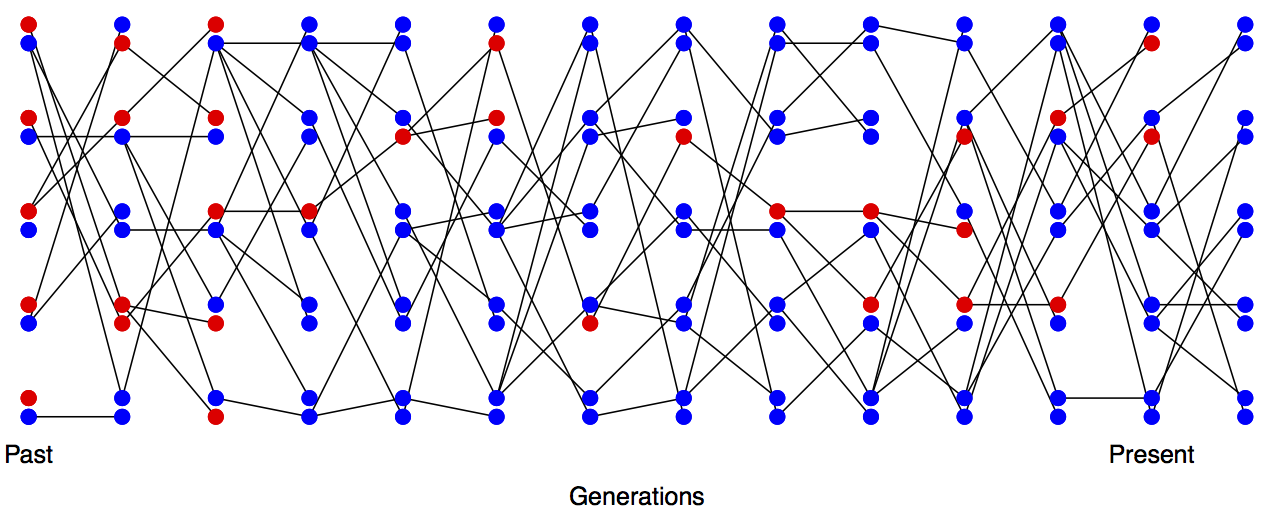
\includegraphics[width= \textwidth]{figures/Loss_of_he_col_two_alleles.png}
\end{center}
\caption{Loss of heterozygosity over time, in the absence of new
  mutations. A diploid population of 5 individuals over the
  generations, with lines showing transmission. In the first
  generation every individual is a heterozygote.} \label{fig:LossHet_two_alleles}
\end{figure} 

\begin{figure}
\begin{center}
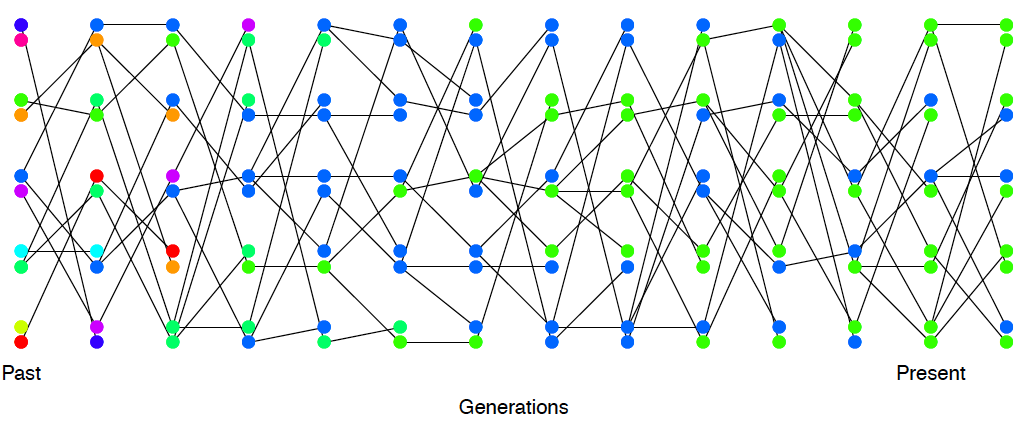
\includegraphics[width= \textwidth]{figures/Loss_of_het_2_many_alleles.png}
\end{center}
\caption{Loss of heterozygosity over time, in the absence of new
  mutations. A diploid population of 5 individuals. In the first generation I colour every allele a different
colour so we can track their descendants.} \label{fig:LossHet_many_alleles}
\end{figure} 


In the next generation ($t+1$) we are looking at the alleles in the
offspring of generation $t$. If we randomly sample two alleles in generation
$t+1$ which had different parental alleles in generation $t$, that
is just like drawing two random alleles from generation $t$. So the
probability that these two alleles in generation $t+1$, that have
different parental alleles in generation $t$, are non-identical is
$H_t$. \\

Conversely, if the two alleles in our pair had the same parental allele in
the proceeding generation (i.e. the alleles are identical by descent
one generation back) then these two alleles must be identical (as we
are not allowing for any mutation). \\



In a diploid population of size $N$ individuals there are $2N$ alleles. The
probability that our two alleles have the same parental allele in the
proceeding generation is $\nicefrac{1}{(2N)}$ and the probability that they have
different parental alleles is is $1-\nicefrac{1}{(2N)}$. So by the above
argument, the expected heterozygosity in generation $t+1$ is
%
\begin{equation}
H_{t+1} = \frac{1}{2N} \times 0 + \left(1-\frac{1}{2N} \right)H_t
\end{equation}
%
Thus, if the heterozygosity in generation $0$ is $H_0$, our
expected heterozygosity in generation $t$ is
%
\begin{equation}
H_t = \left(1-\frac{1}{2N} \right)^tH_0  \label{eqn:loss_het_discrete}
\end{equation}
%
i.e. the expected heterozygosity within our population is decaying
geometrically with each passing generation. If we assume that $\nicefrac{1}{(2N)}
\ll 1$ then we can approximate this geometric decay by an exponential
decay (see Question \ref{geo_question} below), such that
%
\begin{equation}
H_t =H_{0} e^{ - \nicefrac{t}{(2N)} }
\end{equation}
%
i.e. heterozygosity decays exponentially at a rate
$\nicefrac{1}{(2N)}$.

In Figure \ref{fig:LossHet_WF_N50} we show trajectories through time for 40 independently simulated loci drifting in a population of 50 individuals. Each population was started from a frequency of $30\%$ some drift up and some drift down eventually being lost or fixed from the population, but on average, across simulations, the allele frequency doesn't change. We also track heterozygosity, you can see that heterozygosity sometimes goes up, and sometimes goes down, but on average we are loosing heterozygosity, and this rate of loss is well predicted by eqn. \eqref{eqn:loss_het_discrete}. 
\begin{figure}
\begin{center}
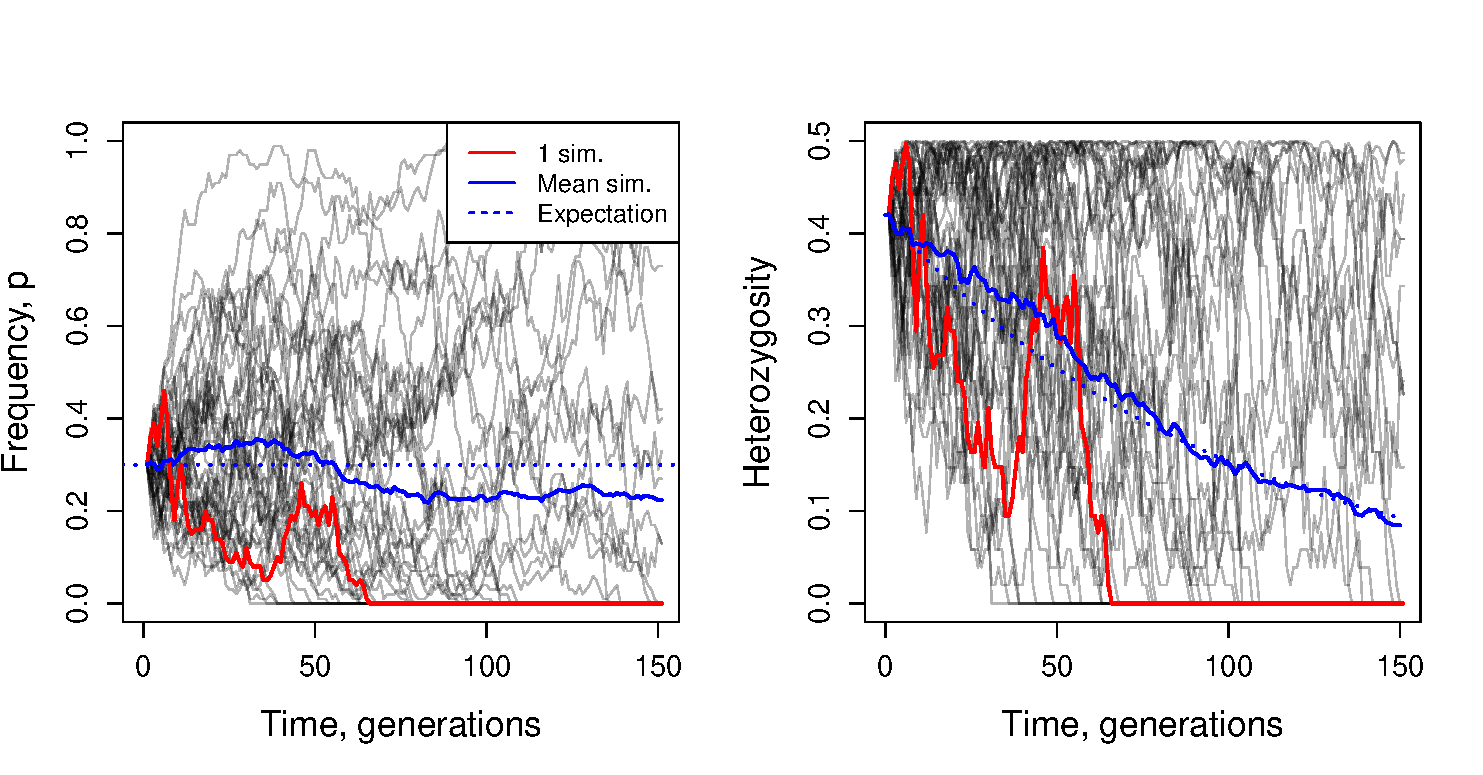
\includegraphics[width= \textwidth]{figures/WF_loss_het/WF_loss_het_N50.pdf}
\end{center}
\caption{Change in allele frequency and loss of heterozygosity over time for 40 replicates. Simulations of genetic drift in a diploid population of 50 individuals, in the absence of new mutations. We start 40 independent, biallelic loci each with an initial allele at 30\% frequency. The left panel shows the allele frequency over time and the right panel shows the heterozygosity over time, with the mean decay matching eqn. \eqref{eqn:loss_het_discrete}.} \label{fig:LossHet_WF_N50}
\end{figure} 


\begin{marginfigure}
\begin{center}
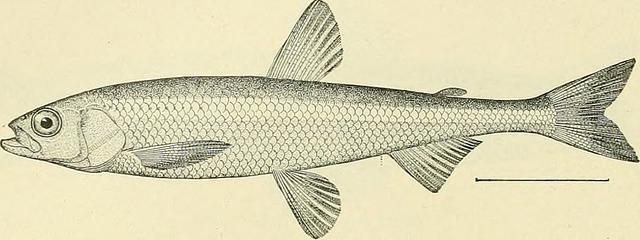
\includegraphics[width= \textwidth]{illustration_images/Genetic_drift/smelt/20497452375_9be855d9ff_z.jpg}
\end{center}
\caption{Pond smelt ({\it Hypomesus olidus}), a close relative of delta smelt. Bulletin of the United States Fish Commission. 1906.} \label{fig:smelt}
\end{marginfigure} 

\begin{question} You are in charge of maintaining a population of delta smelt in the Sacramento river delta. Using a large set of microsatellites you
  estimate that the mean level of heterozygosity in this population is 0.005.
  You set yourself a goal of maintaining a level of heterozygosity of at least
  0.0049 for the next two hundred years. Assuming that the smelt have a
  generation time of 3 years, and that only genetic drift affects these loci, what is the smallest fully outbreeding population that you would need to maintain to meet this goal?  
\end{question}

Note how this picture of decreasing heterozygosity stands in contrast to the
consistency of Hardy-Weinberg equilibrium from the previous chapter. 
However, our Hardy-Weinberg \emph{proportions} still hold in forming each new generation. As the offsprings' genotypes in the next generation ($t+1$) represent a random
draw from the previous generation ($t$), if the parental frequency is $p_t$, we \emph{expect} a proportion $2p_t(1-p_t)$ of our offspring to be
heterozygotes (and HW proportions for our homozygotes). However, because population size is finite, the
observed genotype frequencies in the offspring will (likely) not match exactly with our expectations. As our genotype frequencies likely change slightly due
to sampling, biologically this reflects random variation in family size
and Mendelian segregation, the allele frequency will changed. Therefore, while each generation represents a sample from
Hardy-Weinberg proportions based on the generation before, our
genotype proportions are not at an equilibrium (an unchanging state) as the
underlying allele frequency changes over the generations. We'll develop some mathematical models for these allele
frequency changes later on. For now, we'll simply note that
under our simple model of drift (formally the Wright Fisher model), our
allele count in the $t+1^{th}$ generation represents a binomial sample
(of size $2N$) from the population frequency $p_t$ in the previous
generation.  If you've read to here, please email Prof Coop a picture of JBS Haldane in a striped suit with the title "I'm reading the chapter 3 notes''. (It's well worth googling JBS Haldane and to read more about his life; he's a true character and one of the last great polymaths. )

% generation $t$ may differ
%from that of $t+1$. We'll develop some mathematical models for these allele
%frequency changes 
 %from the previous generation we are
%drawing alleles at random from the  
%Here, the
%freqeuncy of each genotype will likely change, due to chance fluctuations in
%the underlying allele frequency $p$. While within a single generation
%Hardy--Weinberg proportions are maintained (at least approximately), across
%generations the genotypic frequencies change with allele frequency. The change
%in allele frequencies is due to drift: due to random variation in family size
%and Mendelian segregation, the allele frequency in generation $t$ may differ
%from that of $t+1$. We'll develop some mathematical models for these allele
%frequency changes later on.


\begin{marginfigure}[6cm]
\begin{center}
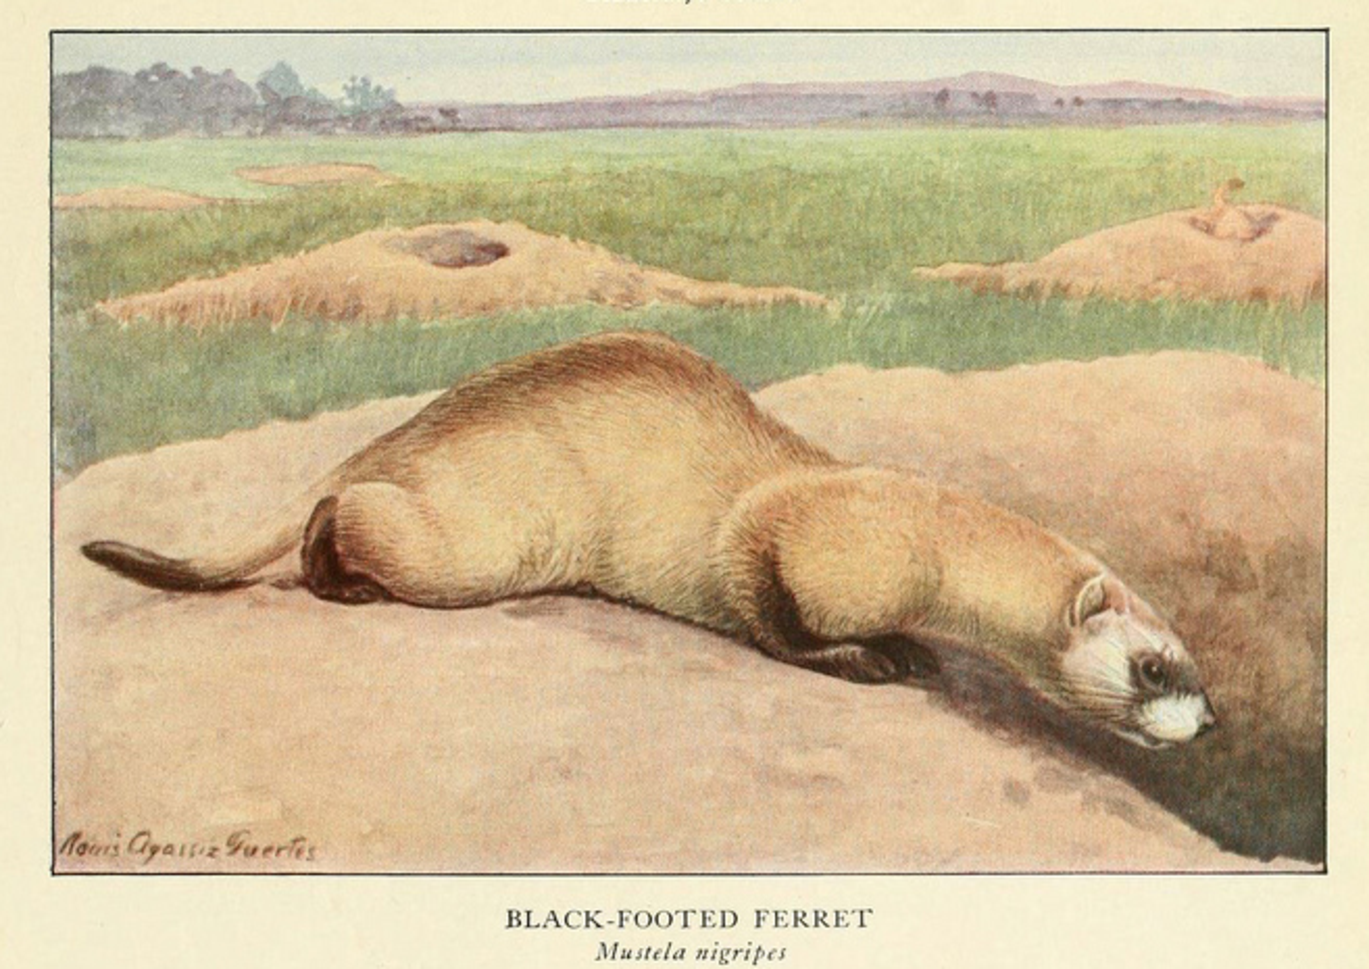
\includegraphics[width=\textwidth]{illustration_images/Genetic_drift/Black_footed_ferrets/Black_footed_ferret.pdf}
\end{center}
\caption{The black-footed ferret ({\it M. nigripes}). Wild animals of North America, The National geographical
  society, 1918. BHL} \label{fig:black_footed_ferret}  
\end{marginfigure} 

\begin{figure}
\begin{center}
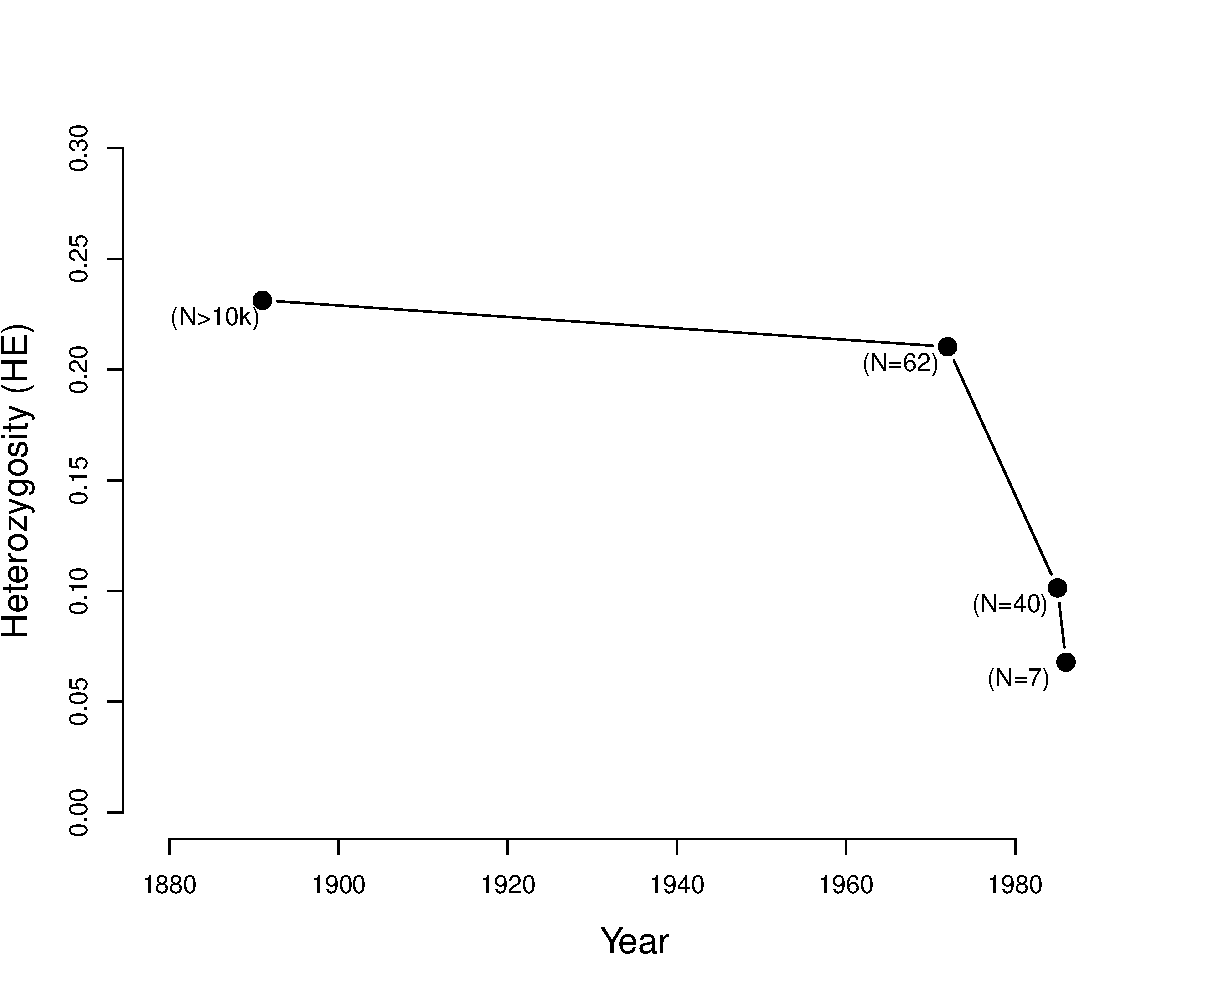
\includegraphics[width= \textwidth]{Journal_figs/genetic_drift/black_footed_ferrets/black_footed_ferrets_He.pdf}
\end{center}
\caption{Loss of heterozygosity in the Black-footed Ferrets in their declining population. Data from \citet{Wisely:02}.} \label{fig:LossHet_ferrets}  
\end{figure} 

To see how a decline in population size can affect levels of
heterozygosity, let's consider the case of black-footed ferrets ({\it Mustela nigripes}). The black-footed ferret population has declined dramatically through the twentieth century due
to destruction of their habitat.  In 1979, when the last known black-footed ferret died in captivity, they were thought to be
extinct. In 1981, a very small wild population was rediscovered ($40$ individuals), but in 1985 this population 
suffered a number of disease outbreaks. All of the $18$ remaining wild individuals
were brought into captivity, 7 of which
reproduced. Thanks to intense captive breeding efforts and conservation work, a
wild population of over 300 individuals has been established
since. However, because all of these individuals are descended from
those 7 individuals who survived the bottleneck, diversity levels
remain low.  \citeauthor{Wisely:02} measured heterozygosity at a number
of microsatellites in individuals from museum collections, showing the sharp drop in diversity as population sizes crashed (see Figure \ref{fig:LossHet_ferrets}).

\begin{question} \label{geo_question} In mathematical population genetics, a
  commonly used approximation is $(1-x) \approx e^{-x}$ for $x << 1$ (formally,
  this follows from the Taylor series expansion of $\exp(-x)$, ignoring second
  order and higher terms of $x$).  This approximation is especially useful for approximating a geometric
  decay process by an exponential decay process, e.g. $(1 - x)^t \approx e^{-xt}$. Using your calculator, or R, check how good of an approximation this is compared to the exact expression for two values of x, $x = 0.1$, and $0.01$, across two different values of t, $t=5$ and $t=50$. I.e. calculate both expressions for these values, hand in your answers and briefly comment on your results. 
 
  %Do this by plotting the geometric decay as
 % points, and the exponential decay as a curve, using different colors for each
 % of these three values of x. Note that you should have a discrete timescale for the
 % geometric decay (e.g. using \texttt{t=seq(0, 18)}) and a near continuous scale
 % for the exponential decay (e.g. using \texttt{t=seq(0, 18, length.out=100)}.
%  Print off your graph and hand it in with your homework. 
    % max <- 18; x <- seq(0, max); x1 <- seq(0, max, length.out=100); plot(x, (1-0.5)^x, col='purple', pch=19); lines(x1, exp(-0.5*x1), col='purple'); points(x, (1-0.1)^x, pch=19, col='orange'); lines(x1, exp(-0.1*x1), col='orange'); points(x, (1-0.01)^x, pch=19, col='green'); lines(x1, exp(-0.01*x1), col='green') # messy but works
\end{question}

\subsection{Levels of diversity maintained by a balance between
 mutation and drift} \label{DriftMutationBalance}

Next we're going to consider the amount of neutral polymorphism that can be maintained in a population as a balance between genetic drift removing variation and mutation introducing new neutral variation, see Figure \ref{fig:Mut_Sel_balance} for an example. Note in our example, how no-one allele is maintained at a stable equilibrium, rather an equilibrium level of polymorphism is maintained by a constantly shifting case of alleles. 

\begin{figure} \begin{center} 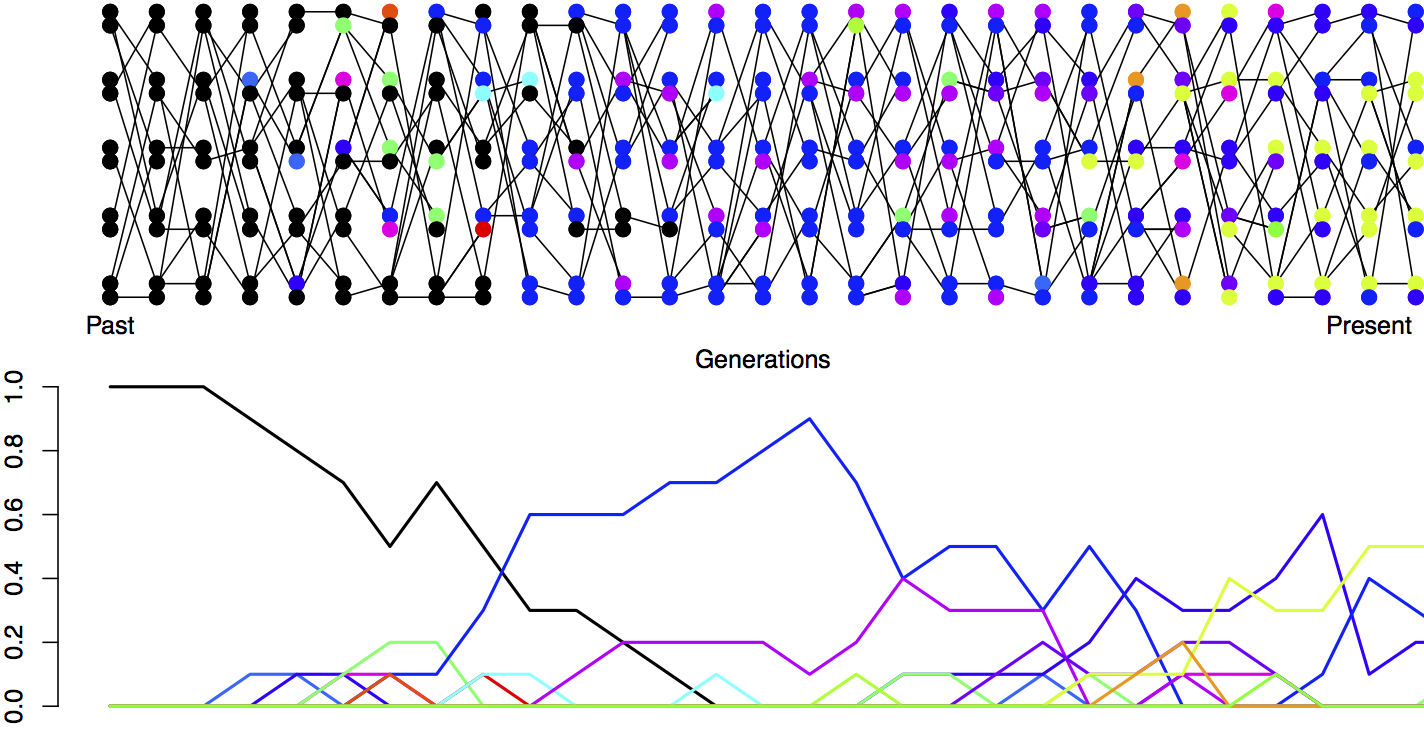
\includegraphics[width= 0.8
\textwidth]{figures/Mut_drift_balance.png} \end{center} \caption{Mutation-drift
balance. A diploid population of 5 individuals. In the first generation
everyone has the same allele (black). Each generation the transmitted allele
can mutate and we generate a new colour. In the bottom plot, I trace the
frequency of alleles in our population over time. The mutation rate we use is very high, simply to maintain diversity in this small population.} \label{fig:Mut_Sel_balance}
\end{figure} 

\paragraph{The neutral mutation rate.} 
We'll first want to consider the rate at which neutral mutations arise in the population.Thinking back to our discussion of the neutral theory of molecular evolution, let's suppose that there are only two classes of mutation that can arise in our genomic region of interest: neutral mutations and highly deleterious mutations. The total mutation rate at our locus is $\mu_T$ per generation, i.e. per transmission from parent to child. A fraction $C$ of our mutations are new alleles that are highly deleterious and so quickly removed from the population. We'll call this $C$ parameter the constraint, and it will differ according to the genomic region we consider.  The remaining fraction $(1-C)$ are our neutral mutations, such that our neutral mutation rate is 
\begin{equation}
\mu = (1-C) \mu_T
\end{equation}
This is the per generation rate.

\begin{question}
It's worth taking a minute to get familiar with both how rare, and how common, mutation is. The per base pair mutation rate in humans is around $1.5 \times 10^{-8}$ per generation. That means, on average, we have to monitor a site for $\sim 66.6$ million transmissions from parent to child to see a mutation. Yet populations and genomes are big places, so mutations are common at these levels. \\
{\bf A)} Your autosomal genome is $\sim 3$ billion base pairs long ($3 \times 10^9$). You have two copies, the one you received from your mum and one from your dad. What is the average (i.e. the expected) number of mutations that occurred in the transmission from your mum and your dad to you?\\
{\bf B)} The current human population size is $\sim 9$ billion individuals. How many times, at the level of the entire human population, is a single base-pair mutated in the transmission from one generation to the next? 
\end{question}
\paragraph{Levels of heterozygosity maintained as a balance between mutation and selection.}





Looking backwards in time from one generation to the previous generation, we are going to say that two alleles which have the same parental allele (i.e. find their common ancestor) in the preceding generation have \emph{coalesced}, and refer to this
event as a \emph{coalescent event}.

The probability that our pair of randomly sampled alleles have coalesced in the
preceding generation is $\nicefrac{1}{(2N)}$, the probability that our pair of
alleles fail to coalesce is $1-\nicefrac{1}{(2N)}$. 

The probability that a mutation changes the identity of the
transmitted allele is $\mu$ per generation. So the probability of no
mutation occurring is $(1-\mu)$. We'll assume that when a mutation
occurs it creates some new allelic type which is not present in the
population. This assumption (commonly called the infinitely-many-alleles model) makes the math slightly cleaner, and also
is not too bad an assumption biologically. See Figure
\ref{fig:Mut_Sel_balance} for a depiction of mutation-drift balance in
this model over the generations.

This model lets us calculate when our two alleles last shared a common
ancestor and whether these alleles are identical as a result of
failing to mutate since this shared ancestor.  For example, we can work out the probability that our
two randomly sampled alleles coalesce $2$ generations in the past
(i.e. they fail to coalesce in generation $1$ and then coalesce in
generation $2$), and
that they are identical as
\begin{equation}
\left(1- \frac{1}{2N} \right) \frac{1}{2N} (1-\mu)^4
\end{equation}
Note the power of $4$ is because our two alleles have to have failed
to mutate through $2$ meioses each. 

More generally, the probability that our alleles coalesce in generation
$t+1$ (counting backwards in time) and are identical due to no mutation to either allele in the
subsequent generations is
%
\begin{equation}
P(\textrm{coal. in t+1 \& no mutations}) =  \frac{1}{2N} \left(1- \frac{1}{2N} \right)^t \left(1-\mu \right)^{2(t+1)}
\end{equation}
%
To make this slightly easier on ourselves let's further assume that $t
\approx t+1$ and so rewrite this as:
\begin{equation}
P(\textrm{coal. in t+1 \& no mutations}) \approx \frac{1}{2N} \left(1- \frac{1}{2N} \right)^t \left(1-\mu \right)^{2t}
\end{equation}
%

This gives us the approximate probability that two alleles will coalesce in the
$(t+1)^\text{th}$ generation. In general, we may not know when two alleles may
coalesce: they could coalesce in generation $t=1, t=2, \ldots $, and so on.
Thus, to calculate the probability that two alleles coalesce in \emph{any}
generation before mutating, we can write:

\begin{align*}
  P(\textrm{coal. in any generation \& no mutations}) \approx & P(\textrm{coal. in} \; t=1 \; \textrm{\& no mutations}) \; + \\ 
&  P(\textrm{coal. in} \; t=2 \; \textrm{\& no mutations}) + \ldots \\
  %P(\textrm{coal. in} \; t=3 \; \textrm{\& no mutations})  +\ldots \\
  = & \sum_{t=1}^\infty P(\textrm{coal. in } \; t \; \textrm{generations \& no mutation})
\end{align*}
%
which follows from basic probability and the fact that coalescing in a particular generation is mutually exclusive with coalescing in a different generation.

While we could calculate a value for this sum given $N$ and $\mu$, it's
difficult to get a sense of what's going on with such a complicated expression.
Here, we turn to a common approximation in population genetics (and all applied
mathematics), where we assume that $\nicefrac{1}{(2N)} \ll 1$ and $\mu \ll 1$.
This allows us to approximate the geometric decay as an exponential decay.
Then, the probability two alleles coalesce in generation $t+1$ and don't mutate
can be written as:
%
\begin{align} P(\textrm{coal. in t+1 \& no mutations}) &\approx \frac{1}{2N}
\left(1- \frac{1}{2N} \right)^t \left(1-\mu \right)^{2t} \\ 
& \approx \frac{1}{2N} e^{-t/(2N)} e^{-2\mu t } \\
&=\frac{1}{2N} e^{-t(2\mu+1/(2N))} \end{align} 
%
Then we can approximate the summation by an integral, giving us:
%

\begin{equation}
\frac{1}{2N} \int_0^{\infty} e^{-t(2\mu+1/(2N))} dt =
\frac{1/(2N)}{1/(2N)+2\mu} = \frac{1}{1+4N\mu}
\end{equation}

The equation above gives us the probability that our two alleles coalesce at some point
in time, and do not mutate before reaching their common
ancestor. Equivalently, this can be thought of as the probability our two
alleles coalesce \emph{before} mutating, i.e. that they are homozygous. 

Then, the complementary probability that our pair of alleles are non-identical
(or heterozygous) is simply one minus this. The following equation gives the equilibrium
heterozygosity in a population at equilibrium between mutation and drift:

\marginnote{This result was derived by \citet{kimura1964number} and \citet{malecot:48}  \citep[see][for an English translation, the lack of earlier translation meant this result was missed]{malecot:69}. Technically we're assuming that every new mutation creates a new allele, the so-called "infinitely many alleles" model, otherwise our pair of sequences could be identical due to repeat or back mutation. See this GENETICS \href{http://genestogenomes.org/kimura-crow-infinite-alleles/}{blog post} and \citet{ewens2016motoo} for a nice discussion of the history. }

\begin{equation}
  H = \frac{4N\mu}{1+4N\mu} \label{eqn:hetero}
\end{equation}
 compound parameter $4N\mu$, the population-scaled mutation rate,
will come up a number of times so we'll give it its own name:
\begin{equation}
\theta = 4N\mu
\end{equation}

So all else being equal, species with larger population sizes should
have proportionally higher levels of neutral polymorphism.  

\begin{question}
The sequence-level heterozygosity in {\it Capsella grandiflora} (grand shepherd's purse) is $\sim 2\%$ per base. Assuming a mutation rate of $10^{-9} bp^{-1}$ per generation, what is your estimate of the population size of {\it C. grandiflora}?  
\end{question}

\subsection{The effective population size}
\marginnote{the effective population size ($N_e$) is the population size that
would result in the same rate of drift in an idealized population of constant size (following our modeling
assumptions)
as that observed in our true population .}

In practice, populations rarely conform to our assumptions of being constant in size with low variance in reproductive success. Real populations experience dramatic fluctuations in size, and there is
often high variance in reproductive success. Thus rates of drift in
natural populations are often a lot higher than the census population
size would imply. See Figure \ref{fig:LossHet_varying_pop}  for a depiction of
a repeatedly bottlenecked population losing diversity at a fast rate.

\begin{figure}
\begin{center}
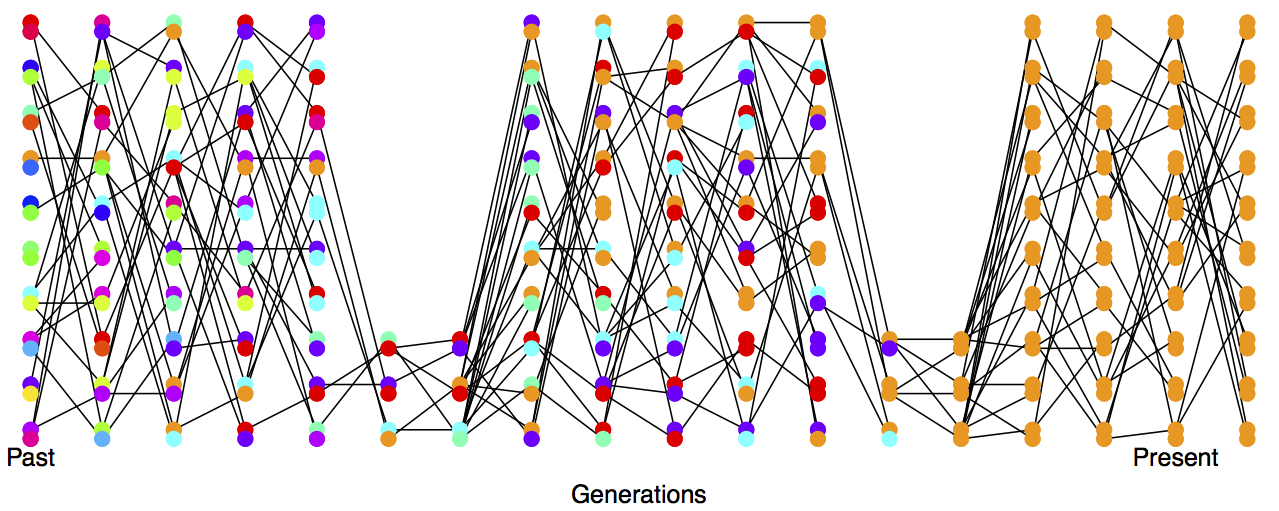
\includegraphics[width= \textwidth]{figures/Loss_of_he_col_alleles_varying_pop_dark.png}
\end{center}
\caption{Loss of heterozygosity over time in a bottlenecking population. A diploid population of 10 individuals, that bottlenecks
  down to three individuals repeatedly. In the first generation, I colour every allele a different
colour so we can track their descendants. There are no new
  mutations.} \label{fig:LossHet_varying_pop}  
\end{figure} 


To cope with this discrepancy, population geneticists often invoke the concept of
an \emph{effective population size} ($N_e$). In many situations (but not all), departures from model assumptions can be captured by substituting $N_e$ for $N$.
\\


If population sizes vary rapidly in size, we can (if certain conditions are met) replace our population size by the harmonic mean population size.
Consider a diploid population of variable size, whose size is $N_t$ $t$ generations into the
past. The probability our pairs of alleles have not coalesced by generation $t$ is
given by
\begin{equation}
\prod_{i=1}^{t} \left(1-\frac{1}{2N_i} \right) \label{eqn:var_pop_coal}
\end{equation}
Note that this simply collapses to our original expression
$\left(1-\frac{1}{2N } \right)^t $ if $N_i$ is constant. Under this model, the rate of loss of heterozygosity in this population is equivalent to
a population of effective size
\begin{equation}
N_e =\frac{1}{\frac{1}{t} \sum_{i=1}^{t} \frac{1}{N_i} }. \label{eq:Ne_harmonic}
\end{equation}
This is the harmonic mean of the varying population size. \sidenote[][-6cm]{
To see this, note that if $1/(N_i)$ is
small, then we can approximate \eqref{eqn:var_pop_coal} using the exponential approximation: 
\begin{equation}
\prod_{i=1}^{t} \exp \left( -\frac{1}{2N_i} \right)   =
\exp \left(- \sum_{i=1}^{t} \frac{1}{2N_i} \right) .
\end{equation}
When we put the product inside the exponent, it becomes a sum.  We can also write the probability of not coalescing by generation $t$ in a population of constant size ($N_e$) as an exponential, so that it takes the same form as the expression above on the right. Comparing the exponent in the two cases, we see
\begin{equation}
\frac{t}{2N_e} = \sum_{i=1}^{t} \nicefrac{1}{2N_i} 
\end{equation}
So that if we want a constant effective population size ($N_e$) that has the same
rate of loss of heterozygosity as our variable population, we need to rearrange and solve this equation to give \eqref{eq:Ne_harmonic}. }


Thus our effective population size, the size of an idealized constant
population which matches the rate of genetic drift, is the harmonic
mean true population size over time. The harmonic mean is very
strongly affected by small values, such that if our population size is
one million $99\%$ of the time but drops to $1000$ every hundred or
so generations, $N_e$ will be much closer to $1000$ than a
million. \\


%would result in the same rate of drift
%Luckily, in many (not all) situations, departures from model assumptions can be captured by substituting Ne for N, i.e., by plugging in a fictitious N that leads to the same level of genetic drift as observed.

\begin{figure}
\begin{center}
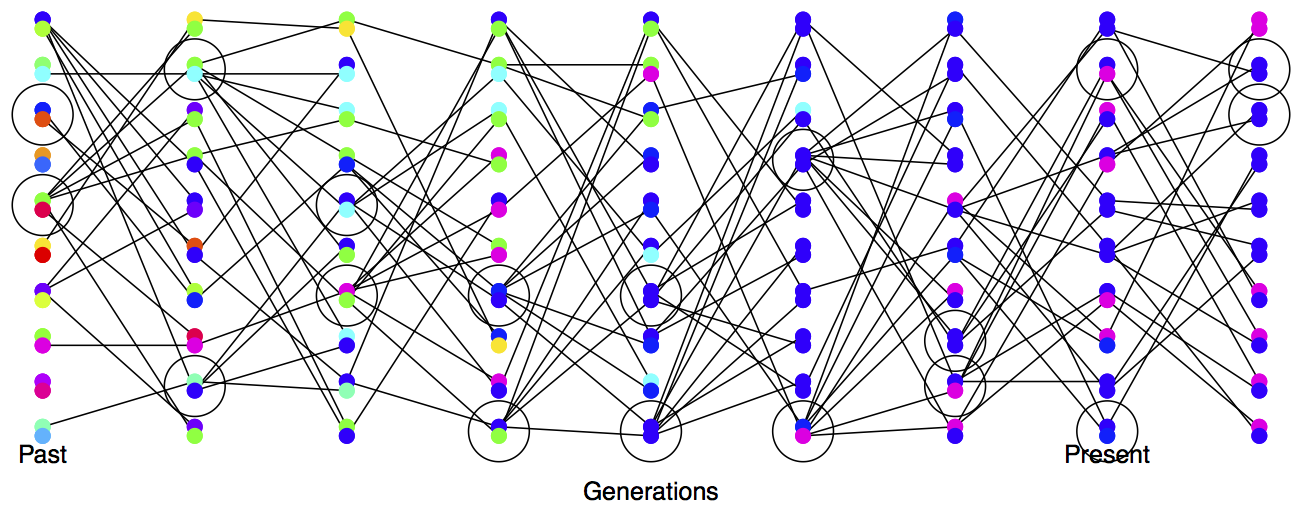
\includegraphics[width= \textwidth]{figures/Loss_of_he_col_alleles_varying_RS.png}
\end{center}
\caption{High variance on reproductive success increases the rate of genetic drift. A diploid population of 10 individuals, where the circled
  individuals have much higher reproductive success. In the first generation I colour every allele a different
colour so we can track their descendants, there are no new
  mutations.} \label{fig:LossHet_varying_RS}
\end{figure} 

Variance in reproductive success will also affect our effective
population size. Even if our population has a large constant size $N$
individuals, if only small proportion of them get to reproduce, then
the rate of drift will reflect this much smaller number of reproducing
individuals. See Figure \ref{fig:LossHet_varying_RS} for a depiction of the higher rate of drift
in a population where there is high variance in reproductive success.

To see one example of this, consider the case where $N_F$ of  females get to reproduce and $N_M$ males get reproduce.
While every individual has a mother an a father, not every individual gets to be a parent. In practice, in many animal species far more females get to reproduce than males, i.e. $NM <N_F$, as a few males get many mating opportunities and many males get no/few mating opportunities \citep[see ][for a broad analysis, and note that there a certainly many exceptions to this general pattern]{janicke:16}. When our two alleles pick an ancestor, $25\%$ of the time our alleles were both in a female ancestor, in which case they are IBD with probability $1/(2N_F)$, and $25\%$ of the time they are both in a
male ancestor, in which case they coalesce with probability
$1/(2N_M)$. The remaining $50\%$ of the time, our alleles trace back to two individuals of different sexes in the prior generation and so cannot coalesce.  Therefore, our probability of coalescence in the preceding generation is 
\begin{equation}
\frac{1}{4}\left(\frac{1}{2N_M} \right)+\frac{1}{4}\left(\frac{1}{2N_F} \right) %=
%\frac{1}{8}\frac{N_F+N_M}{N_FN_M} 
\end{equation}
i.e. the rate of coalescence is the harmonic mean of the two sexes' population sizes, equating this to $\frac{1}{2N_e}$ we find

\begin{marginfigure}
\begin{center}
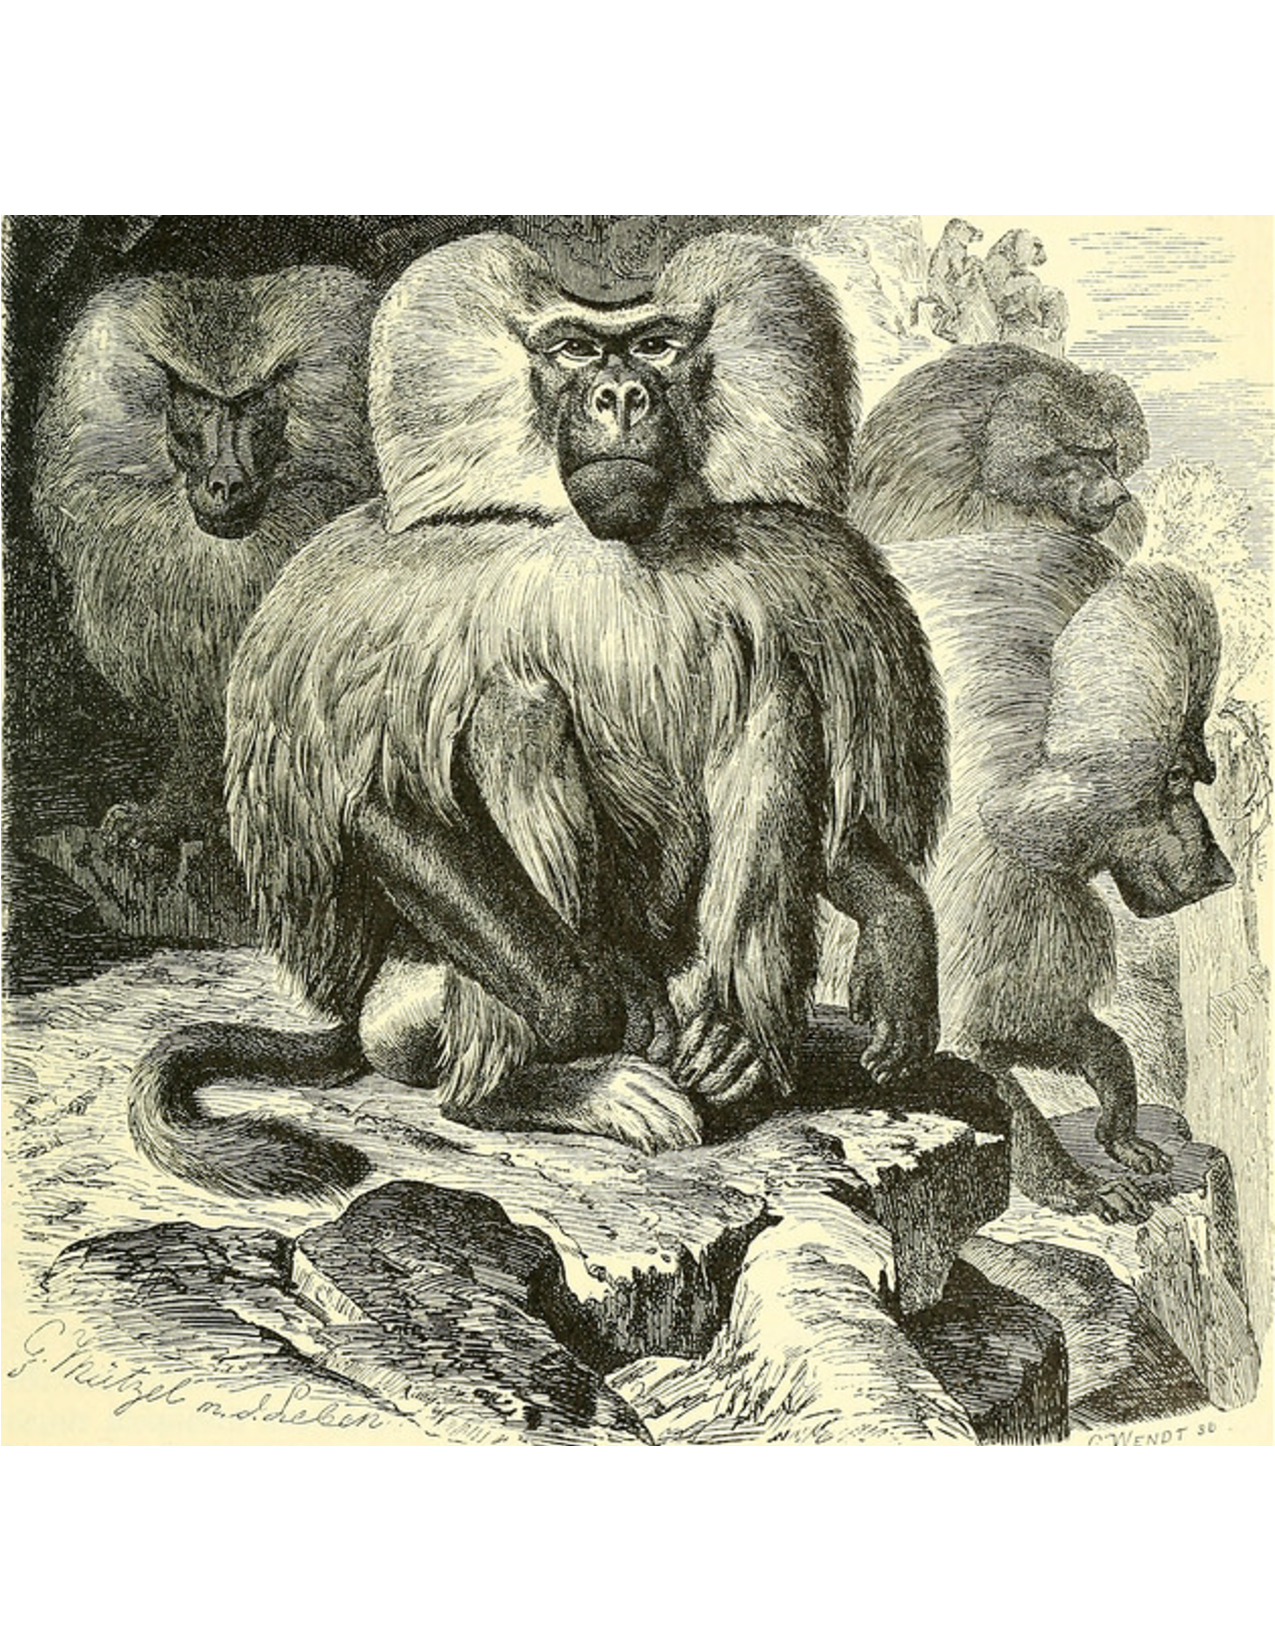
\includegraphics[width= 0.7 \textwidth]{illustration_images/Genetic_drift/Hamadryas_baboon/Hamadryas_baboon.pdf}
\end{center}
\caption{Male Hamadryas baboons. Brehm's Tierleben. Brehm,
  A.E. 1893. Up to ten females live in a harem with a single male.  %Brehm's animal life
} \label{fig:Hamadryas_baboon}  
\end{marginfigure} 

\begin{equation}
N_e = \frac{4N_FN_M}{N_F+N_M}
\end{equation}
Thus if reproductive success is very skewed in one sex (e.g. $N_M \ll
N/2$), our effective population size will be much reduced as a result. For more on how different evolutionary forces affect the rate of genetic drift, and their impact on the effective population size, see \citet{charlesworth:09}.\\

\begin{question}
You are studying a population of 500 males and 500 females Hamadryas baboons. Assume that all of the females but only 1/10 of the males get to mate: 
{\bf A)} What is the effective population size for the autosome?\\
{\bf B)} Do you expect the {\it ratio} of X-chromosome to autosomal diversity to be higher or lower in this species compared to a species where the sexes have more similar variance in reproductive success? Explain the intuition behind your answer.
 \end{question}


\section{The Coalescent and patterns of neutral diversity}

\begin{quote}
"Life can only be understood backwards; but it must be lived
forwards." -- Kierkegaard
\end{quote}

\paragraph{Pairwise Coalescent time distribution and the number of
 pairwise differences.}
Thinking back to our calculations we made about the loss of neutral heterozygosity
and equilibrium levels of diversity (in Sections \ref{LossofHet} and \ref{DriftMutationBalance}), you'll note that we could first specify
which generation a pair of sequences coalesce in, and then calculate
some properties of heterozygosity based on that. That's because neutral
mutations do not affect the probability that an individual transmits
an allele, and so don't affect the way in which we can trace ancestral lineages
back through the generations. \\


As such, it will often be helpful to consider the time to the common
ancestor of a pair of sequences, and then think of the impact of that time to coalescence
on patterns of diversity. See Figure \ref{fig:Coalescent_simulation}
for an example of this. 

\begin{figure}
\begin{center}
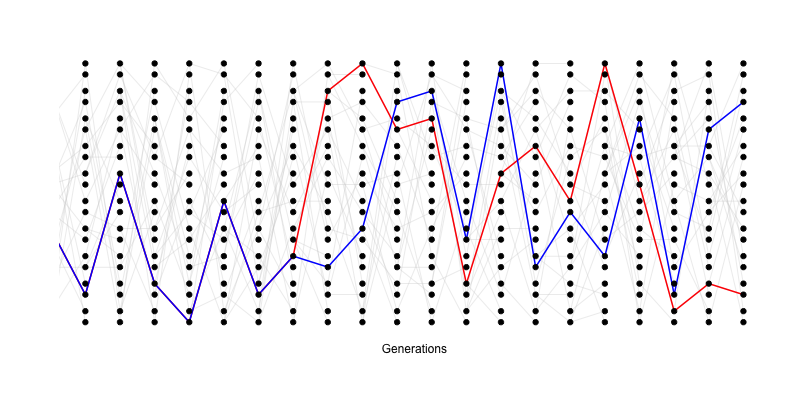
\includegraphics[width=\textwidth]{figures/Coalescent.png}
\end{center}
\caption{A simple simulation of the coalescent process. The simulation
  consists of a diploid population of 10 individuals (20 alleles). In
  each generation, each individual is equally likely to be the parent
  of an offspring (and the allele transmitted is indicated by a light
  grey line).  We track a
  pair of alleles, chosen in the present day, back 14 generations
  until they find a common ancestor.} \label{fig:Coalescent_simulation}
\end{figure}

The probability that a pair of alleles
have failed to coalesce in $t$ generations and then coalesce in the
$t+1$ generation back is 
\begin{equation}
 P(T_2=t+1) = \frac{1}{2N} \left(1- \frac{1}{2N} \right)^{t} \label{eqn:coal_time_dist}
\end{equation}
Thus the coalescent time of our pair of alleles is a Geometrically distributed random variable, where the probability of success is $1/(2N)$; we denote this by $T_2 \sim  \text{Geo}(1/(2N))$.
The expected (i.e. the mean over many replicates) coalescent time of a pair of alleles is then  
\begin{equation}
\E(T_2) = 2N 
\end{equation}
generations.\\

\marginnote{Blurring our eyes a little, we can see  that \ref{eqn:coal_time_dist} is
\begin{equation}
\approx \frac{1}{2N} e^{-t/(2N)} 
\end{equation}
and so think of  a continuous random variable, i.e. we could say that the coalescent time of a pair of sequences ($T_2$) is approximately exponentially distributed with a rate $1/(2N)$, i.e. $T_2 \sim \text{Exp}\left( 1/(2N) \right)$. Formally we can do this by taking the limit of the discrete more carefully. }

Conditional on a pair of alleles coalescing $t$ generations ago,
there are $2t$ generations in which a mutation could occur. If the per
generation mutation rate is $\mu$, then the expected number of
mutations between a pair of alleles coalescing $t$ generations ago is
$2 t\mu$ (the alleles have gone through a total of $2t$ meioses since they last shared a common ancestor). So we can write the expected
number of mutations ($S_2$) separating two alleles drawn at random from the
population as %\erin{I added subscript 2 to all the T's, which I think is appropriate}
\begin{align}
\E(S_2) &= \sum_{t=0}^{\infty} \E(S_2 | T_2=t) P(T_2=t) \nonumber\\
& =\sum_{t=0}^{\infty} 2 \mu t P(T_2=t) \nonumber\\
& =2\mu \E(T_2)  \nonumber\\
& = 4 \mu N 
\end{align}
 
%As our expected coalescent time is $2N$ generations (which follows from the expected value of exponential distributions), the expected
%number of mutations separating two alleles drawn at random from the
%population is
%
%\begin{align}
 % \E(j) &= 2\mu\E(t) \\ \nonumber
 % &= 4N\mu \\
 % &= \theta \nonumber
%\end{align}
We'll assume that mutation is rare enough that it never happens at the same basepair twice, i.e. no multiple hits, such that we get to see all of the mutation events that separate our pair
of sequences \sidenote{This is called the infinitely-many-sites assumption,
which should be fine if $N\mu_{BP} \ll 1$, where $\mu_{BP}$ is the mutation rate per base pair).} Thus the number of
mutations between a pair of sites is the observed number of
differences between a pair of sequences. In the previous chapter we denote the observed number of pairwise differences at putatively neutral
sites separating a pair of sequences as $\pi$ (we usually average this over a
number of pairs of sequences for a region). Therefore, under our simple, neutral, constant population-size model we expect
\begin{equation}
\E(\pi) = 4 N \mu = \theta
\end{equation}
So we can get an empirical estimate of $\theta$ from
$\pi$, let's call this $\widehat{\theta}_{\pi}$, by setting $\widehat{\theta}_{\pi}=\pi$., i.e. our observed level of pairwise genetic diversity.  If we
have an independent estimate of $\mu$, then from setting $\pi =\widehat{\theta}_{\pi} = 4N\mu$ we can furthermore obtain an estimate of the population
size $N$ that is consistent with our levels of neutral polymorphism. If we estimate the population size this way, we should call it the effective coalescent population size ($N_e$). It's best to think about $N_{e}$ estimated from neutral diversity as a long-term, effective population size for the species, but there's a boat load of caveats that come along with that assumption. For example, past bottlenecks and population expansions are all subsumed into a single number and so this estimated $N_{e}$ may not be very representative of the population size at any time. That said, it's not a bad place to start when thinking about the rate of genetic drift for neutral diversity in our population over long time-periods. \sidenote{Up to this point we've been describing only neutral processes, however, selection can also alter levels of polymorphism. For example, if some synonymous sites directly experience selection, then even if we use $\pi$ calculated for on synonymous changes we may underestimate the coalescent effective population size. As we'll see later in the notes, selection at linked sites can also impact neutral diversity. As such, if we can, we may want to use genomic sites subject to the weakest selective constraints, and also far from gene-dense or otherwise very constrained regions of the genome, to estimate $N_e$ from $\pi$. But even then caution is warranted. } 

Lets take a moment to distinguish our expected heterozygosity (eqn. \ref{eqn:hetero}) from our expected number of pairwise differences ($\pi$). Our expected heterozygosity is the probability that two alleles at a locus, sampled from a population at random, are different from each other. If one or more mutations have occurred since a pair of alleles last shared a common ancestor, then our sequences will be different from each other. On the other hand, our $\pi$ measure keeps track of the average total number of differences between our loci. As such, $\pi$ is often a more useful measure, as it records the number of differences between the sequences, not just whether they are different from each other (however, for certain types of loci, e.g. microsatellites, heterozygosity is often used as we cannot usually count up the minimum number of mutations in a sensible way). In the case where our locus is a single basepair, the two measures will usually be close to one another, as $H \approx \theta$ for small values of $\theta$. For example, comparing two sequences at random in humans, $\pi \approx 1/1000$ per basepair, and the probability that a specific base pair differs between two sequences is $\approx 1/1000$. However, these two quantities start to differ from each other when we consider regions with higher mutation rates. For example, if we consider a 10kb region, our mutation rate will 10,000 times larger than a single base pair. For this length of sequence the probability that two randomly chosen haplotypes differ is quite different from the number of mutational differences  between them. (Try a mutation rate of $10^{-8}$ per base and a population size of $10,~000$ in our calculations of $\E[\pi]$ and H to see this.)

%\erin{can you give an intuitive example when per bp $\pi$ is very different from heterozygosity? Or is this distinction really just key when we're talking about larger loci?}

\begin{marginfigure}
\begin{center}
  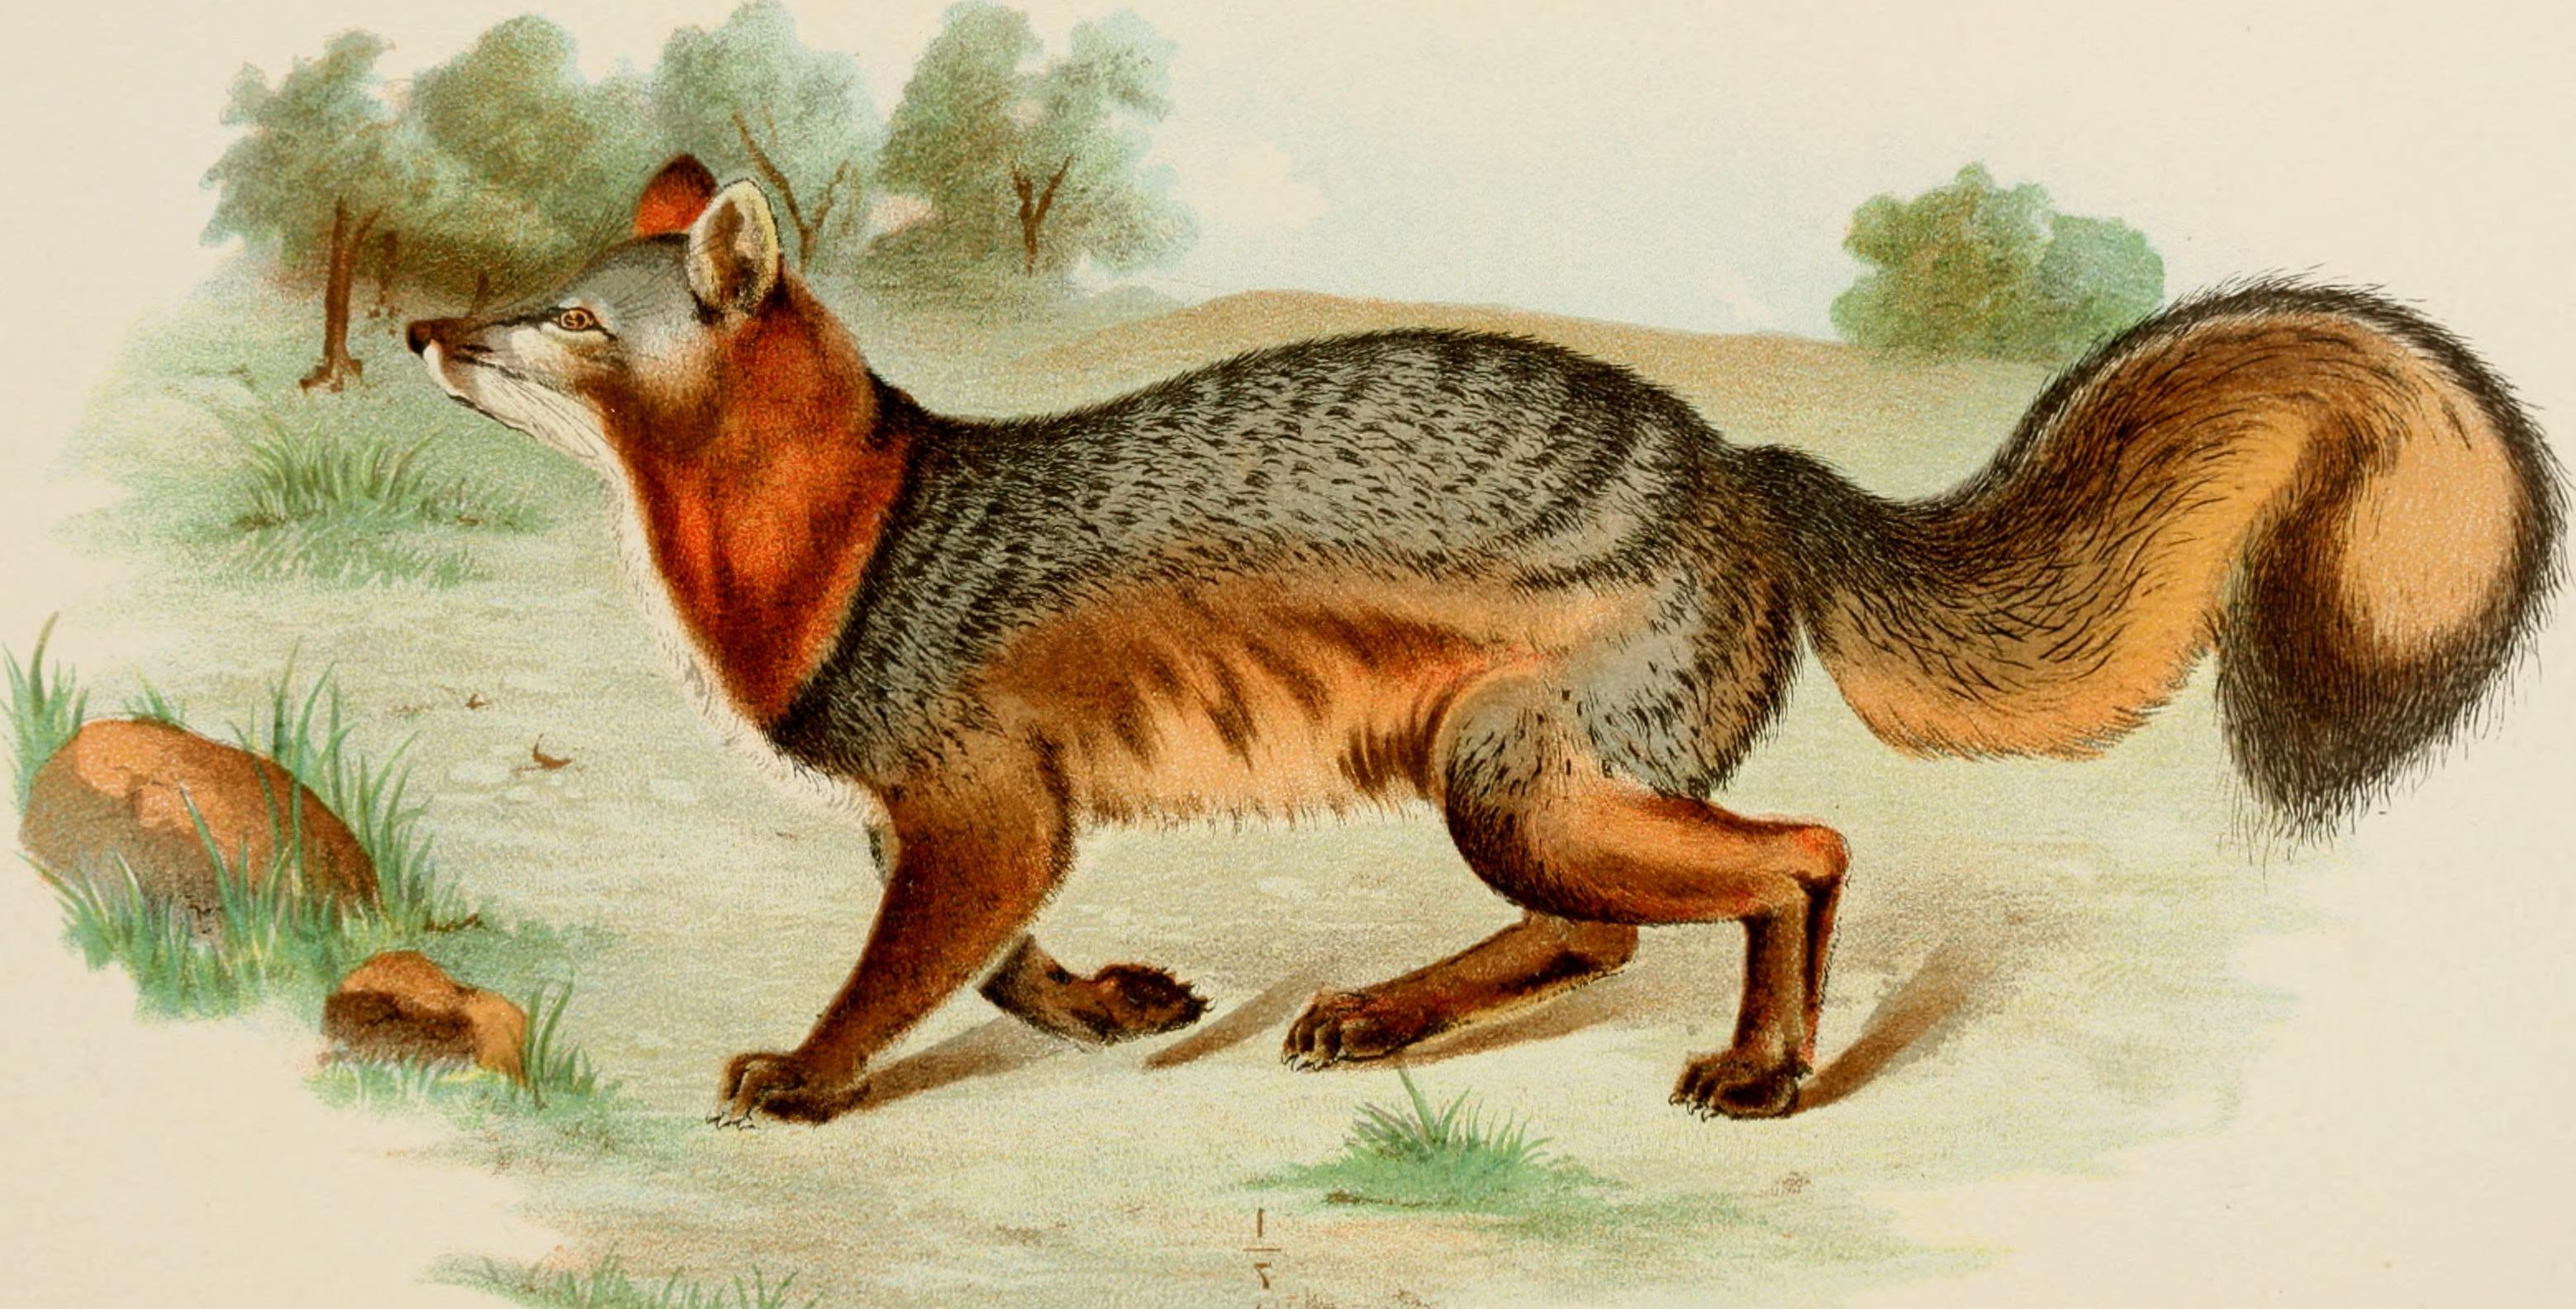
\includegraphics[width =
  \textwidth]{illustration_images/Quant_gen/Grey_fox/14770789583_4db7ec5164_o.jpg}  %https://www.flickr.com/photos/internetarchivebookimages/14770789583/in/photolist-axdicF-ovfa8V-odM3sY-bCrnQ8-ovgYXn-tiQfMQ-odMpu5-x1xCJu-wQ7qT7-wE7kfs-xEZQd1-wK4YSh-ovWx4g-wpDZzF-xjvQ89-tHDjuS-w9Wit5-xEvyhH-xjCbKD-u4q3Qe
\end{center}
\caption{Gray Fox, {\it Urocyon cinereoargenteiis}. Pearson and Warren. Diseases and enemies of poultry. (1897) BHL.} 
\end{marginfigure}


\begin{question}
\citet{robinson:16} found that the endangered Californian Channel Island fox on San Nicolas had very
low levels of diversity ($\pi =0.000014 \text{bp}^{-1}$) compared to
its close relative the California mainland gray fox ($0.0012\text{bp}^{-1}$). \\
%\bf A How many sites do you expect to differ between two samples
%sequenced over a 100kb region in each of these populations?\\   
{\bf A)} Assuming a mutation rate of $2\times 10^{-8}$ per bp, what
effective population sizes do you estimate for these two populations?
\\
{\bf B)} Why is the effective population size of the Channel Island fox
so low? [Hint: quickly google Channel island foxes to read up on their
history, also to see how ridiculously cute they are.]
\end{question}


\begin{question}
In your own words describe why the coalescent time of a pair of lineages scales linearly with the (effective) population size.
%The long-term $N_e$ estimated from genetic diversity within most human populations is roughly $10,000$, and the generation time of humans is $\sim$30 years. What is the average time, in years, that we have to go back to to find the most recent common ancestor for  a pair of sequences drawn from the same human population?
\end{question}


\paragraph{More details on the pairwise coalescent and the randomness of mutation.}

We've derived the expected number of differences between a pair of sequences and talked about how variable the coalescent time is for a pair of sequences. The mutation process is also very variable; even if two sequences coalesce in the very distant past by chance, they may still be identical in the present if there was no mutation during that time. 

Conditional on the coalescent time $t$, the probability that our pair of alleles are separated by $S_2$ mutations since they last shared a common ancestor is
\begin{equation}
P(S_2 | T_2 = t ) = {2t \choose j} \mu^{j} (1-\mu)^{2t-j}
\end{equation}
i.e. mutations happen in $j$ generations and do not happen in $2t-j$
generations (with ${2t \choose j}$ ways this combination of events can possibly
happen). Assuming that $\mu \ll 1$ and that $2t-j \approx 2t$, then we
can approximate the probability that we have $S_2$ mutations as a
Poisson distribution:
\begin{equation}
P(S_2 | T_2 = t ) = \frac{ (2 \mu t )^{j} e^{-2\mu t}}{j!}
\end{equation}
i.e. a Poisson with mean $2\mu t $. We'll not make much use of this result, but it is very useful in thinking about how to simulate the process of mutation.\\

\section{The coalescent process of a sample of alleles.}

Usually we are not just interested in pairs of alleles, or the
average pairwise diversity. Generally we are interested in the properties of
diversity in samples of a number of alleles drawn from the population.  
Instead of just following a pair of lineages back until they
coalesce, we can follow the history of a sample of alleles back
through the population.

Consider first sampling three alleles at random from the population. The
probability that all three alleles choose exactly the same ancestral allele one
generation back is $\nicefrac{1}{(2N)^2}$. If $N$ is reasonably large, then this
is a very small probability. As such, it is very unlikely that our three alleles
coalesce all at once, and in a moment we'll see that it is safe to ignore such
unlikely events. \\

\begin{figure}
\begin{center}
  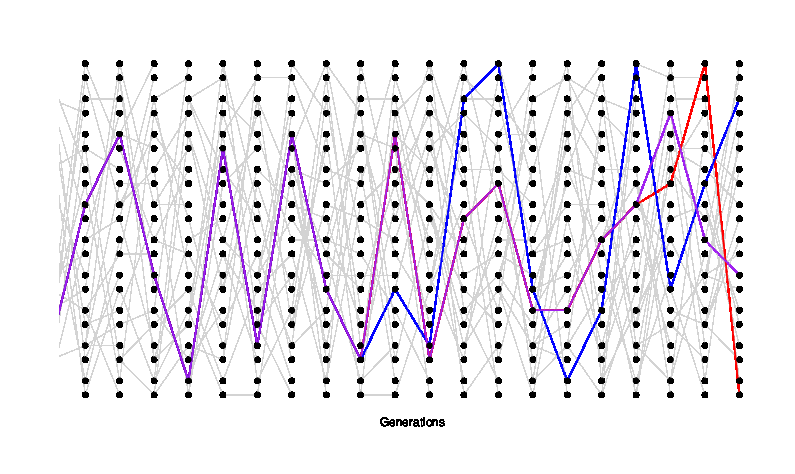
\includegraphics[width = \textwidth]{figures/Coalescent_3.png}
\end{center}
\caption{A simple simulation of the coalescent process for three
  lineages. We track the ancestry of 
  three modern-day alleles, the first pair (blue and purple) coalesce four generations back, after which  
  there are only two independent lineages we are tracking. This pair
  then coalesces twelve generations in the past. Note that different
  random realizations of this process will differ from each other a lot.} \label{fig:Coalescent_simulation_3}
\end{figure}

The probability that a specific pair of alleles find a common ancestor in the
preceding generation is still $\nicefrac{1}{(2N)}$. There are three possible pairs of
alleles, so the probability that no pair finds a common ancestor in the preceding generation is
\begin{equation}
\left(1-\frac{1}{2N} \right)^3 \approx \left( 1- \frac{3}{2N} \right)
\end{equation}
In making this approximation we are multiplying out the right hand-side
and ignoring terms of $1/N^2$ and higher. See
Figure \ref{fig:Coalescent_simulation_3} for a random realization of this process. \\

More generally, when we sample $i$ alleles there are ${i \choose 2}$
pairs,\sidenote{said as ``i choose 2''}  i.e. $i(i-1)/2$ pairs. Thus, the probability that no pair
of alleles in a sample of size $i$ coalesces in the preceding generation is
\begin{equation}
\left(1-\frac{1}{(2N)} \right)^{{i \choose
 2}} \approx \left( 1- \frac{{i \choose
 2}}{2N}\right)
\end{equation}
while the probability any pair coalesces is $\approx \nicefrac{2N}{{i \choose
 2}}$.\\

We can ignore the possibility that more than pairs of alleles (e.g. tripletons)
simultaneously coalesce at once as terms of $\nicefrac{1}{N^2}$ and higher
can be ignored as they are vanishingly rare. Obviously in reasonable
sample sizes there are many more triples (${i \choose 3}$) and higher order
combinations than there are pairs (${i \choose 2}$), but if $i \ll N$ then we are safe to
ignore these terms.



When there are $i$ alleles, the probability that we wait until the
$t+1$ generation before
any pair of alleles coalesces is
\begin{equation}
P(T_i =t+1) = \frac{{i \choose
 2}}{2N}\left( 1- \frac{{i \choose
 2}}{2N}\right)^{t} \label{eqn:T_i}
\end{equation}
Thus the waiting time to the first coalescent event while there are $i$ lineages is a geometrically distributed random variable with probability of success $\nicefrac{{i \choose 2}}{2N}$, which we denote by
\begin{equation}
T_i \sim \text{Geo}
\left(  \nicefrac{{i \choose
      2}}{2N} \right).
\end{equation}
The mean waiting time till any of pair within our
 sample coalesces is 
\begin{equation}
\E( T_i) = \frac{2N}{{i \choose  2}}  \label{eqn:E_T_i}
\end{equation}
\marginnote{
To see the continuous time  version of this, note that \eqref{eqn:T_i} is
\begin{equation} 
\approx  \frac{{i \choose
 2}}{2N} \exp \left( - \frac{{i \choose
 2}}{2N} t \right)
\end{equation}
The waiting time $T_i$ to the first coalescent event in a sample
of $i$ alleles is thus exponentially distributed with rate $\nicefrac{{i \choose
 2}}{2N}$, i.e. $T_i \sim \text{Exp}\left(\nicefrac{{i \choose
 2}}{2N} \right)$. }
After a pair of alleles first finds a common ancestral allele some
number of generations back in the past, we only have to keep
track of that common ancestral allele for the pair when looking further into the past. Thus when a pair
of alleles in our sample of $i$ alleles coalesces, we then switch to
having to follow $i-1$ alleles back in time. Then when a pair of these $i-1$
alleles coalesce, we then only have to follow $i-2$ alleles back. This
process continues until we coalesce back to a sample of two, and from
there to a single most recent common ancestor (MRCA).\\


\paragraph{Simulating a coalescent genealogy}
To simulate a coalescent genealogy at a locus for a sample of $n$ alleles we therefore simply follow the following
algorithm:
\begin{enumerate}
\item Set $i=n$.
\item Simulate a random variable to be the time $T_i$ to the next coalescent event from $T_i \sim
  \text{Exp}\left(\nicefrac{{i \choose
 2}}{2N} \right)$
\item Choose a pair of alleles to coalesce at random from all possible
 pairs.
\item Set $i=i-1$
\item Continue looping steps 1-3 until $i=1$, i.e. the most recent
 common ancestor of the sample is found.
\end{enumerate}
By following this algorithm we are generating realizations of the
genealogy of our sample. \\



\subsection{Expected properties of coalescent genealogies and
  mutations.} 

\begin{figure}
\begin{center}
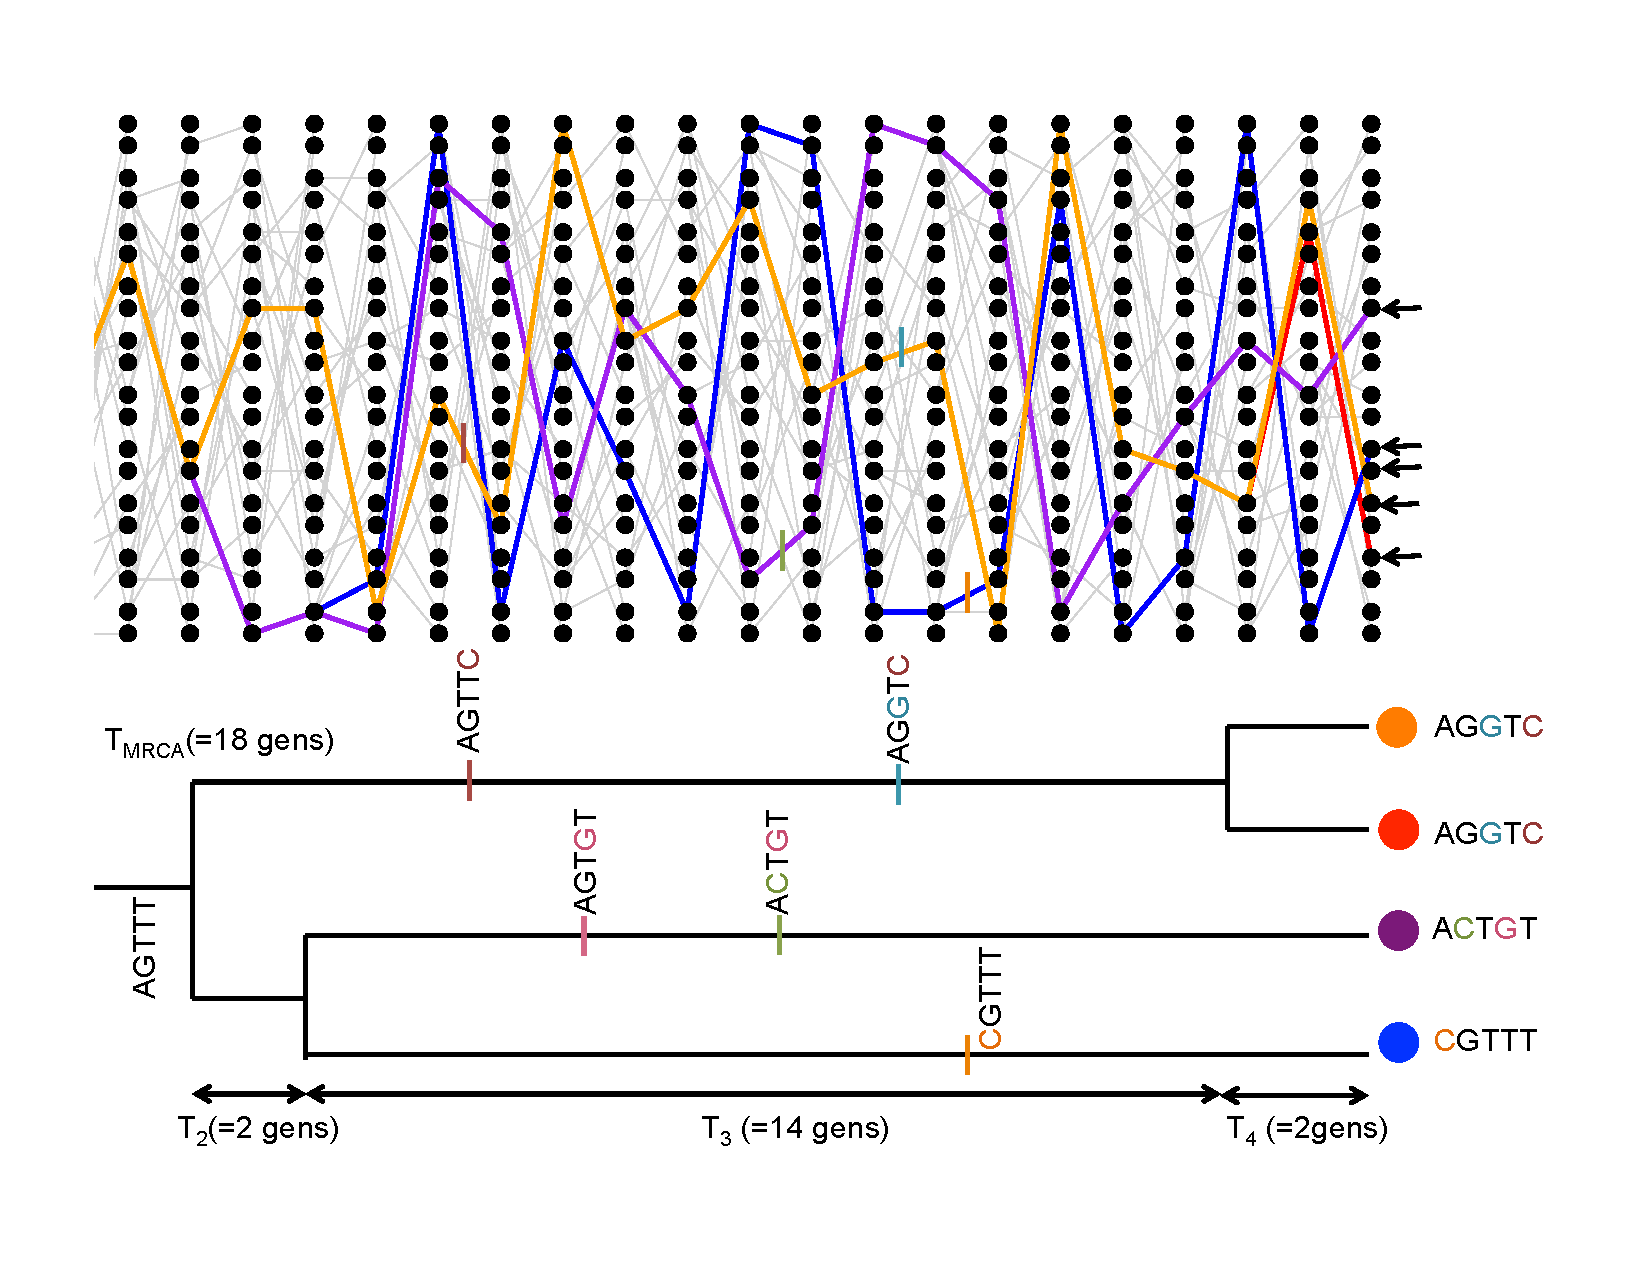
\includegraphics[width= \textwidth]{figures/Coalescent/Coal_w_muts.pdf}
\end{center}
\caption{A simple coalescent tree from a single coalescent simulation, tracing the genealogy of 4 alleles with mutational changes marked with dashes showing transitions away from the MRCA sequence (AGTTT) . The $T_{MRCA}$ is the sum of $T_4$, $T_3$, and $T_2$. The total time in the tree is $T_{tot}=4 T_4+2T_3 + 2T_2= 54$ generations. } \label{fig:Coal_w_muts}
\end{figure}


\paragraph{The expected time to the most recent common ancestor.}
We will first consider the time to the most recent common ancestor of
the entire sample ($T_{MRCA}$). This is
\begin{equation}
T_{MRCA} = \sum_{i=n}^2 T_i
\end{equation}
generations back, where we are summing from $i=n$ alleles counting backwards to $i=2$ alleles (see Figure \ref{fig:Coal_w_muts} for example). As our coalescent times for different $i$ are independent, the expected time to the most recent common ancestor
is
\begin{equation}
\E(T_{MRCA}) = \sum_{i=n}^2 \E(T_i) = \sum_{i=n}^2  2N/{i \choose
 2}
\end{equation}
Using the fact that $\frac{1}{i(i-1)}=\frac{1}{i-1} - \frac{1}{i}$ and a bit of
rearrangement, we can rewrite this as
\begin{equation} 
\E(T_{MRCA}) = 4N\left(1- \frac{1}{n} \right) \label{TMRCA_neutral}
\end{equation}
So the average $T_{MRCA}$ scales linearly with population
size $N$. Interestingly, as we move to larger and larger samples (i.e. $n \gg 1$), the average
time to the most recent common ancestor converges on $4N$. What's
happening here is that in large samples our lineages typically coalesce rapidly
at the start and very soon coalesce down to a much smaller number of
lineages.   \\

\begin{question}
Assume an autosomal effective population of 10,000 individuals (roughly the long-term human estimate) and a generation time of 30 years. What is the expected time to the most recent common ancestor of a sample of 20 people? What is this time for a sample of 500 people?  
\end{question}
\paragraph{The expected total time in a genealogy and the number of
  segregating sites.}

Mutations fall on specific lineages of the coalescent genealogy and are transmitted to all descendants of their lineage. Furthermore, under the infinitely-many-sites assumption, each mutation creates a new segregating site. The mutation process is a
\emph{Poisson process}, and the longer a particular lineage, i.e. the more generations of meioses it represents, the more
mutations that can accumulate on it. The total number of segregating sites in
a sample is thus a function of the \emph{total} amount of time in the
genealogy of the sample, or the sum of all the branch lengths on the genealogical tree,
$T_{tot}$. Our total amount of time in the genealogy is

\begin{equation}
T_{tot} = \sum_{i=n}^2 iT_i
\end{equation}
as when there are $i$ lineages, each contributes a time $T_i$ to the total time (see Figure \ref{fig:Coal_w_muts} for an example). Taking the expectation of the total time in the genealogy,
\begin{equation}
\E(T_{tot}) = \sum_{i=n}^2 i \frac{2N}{{i \choose
 2} } = \sum_{i=n}^2 \frac{4N}{i -1} =\sum_{i=n-1}^1 \frac{4N}{i} \label{eqn:E_T_tot}
\end{equation}
we see that our expected total amount of time in the genealogy scales linearly
with our population size $N$. Our expected total amount of time is also
increasing with sample size $n$, but is doing so very slowly. %To see this
%more carefully, we can see that for large $n$
%\begin{equation}
%\E(T_{tot}) = \sum_{i=n-1}^1 \frac{4N}{i} 
%\end{equation}
\marginnote{To get a better sense of how $T_{tot}$ grows with the sample size, we
  can approximate the sum \ref{eqn:E_T_tot} by an integral, which will work for large $n$. The result is  $\int_1^{n-1} \frac{4N}{i} di
= 4N \log(n-1)$. }
This again follows
from the fact that in large samples, the initial coalescence usually
happens very rapidly, so that extra samples add little to the total
amount of time in the genealogical tree. \\

We saw above that the number of mutational differences between a pair
of alleles that coalescence $T_2$ generations ago was Poisson with a
mean of $2 \mu T_2$, where $2T_{2}$ is the total branch length in this simple 2-sample genealogical tree. A mutation that occurs on any branch of our
genealogy will cause a segregating polymorphism in the sample
(meeting our infinitely-many-sites assumption). Thus, if the total time
in the genealogy is $T_{tot}$, there are $T_{tot}$
generations for mutations. So the total number of mutations
segregating in our sample ($S$) is Poisson with mean $\mu T_{tot}$. Thus the
expected number of segregating  sites in a sample of size $n$ is
\begin{equation}
\E(S) = \mu \E(T_{tot}) = \sum_{i=n-1}^1 \frac{4N\mu }{i} = \theta
\sum_{i=n-1}^1 \frac{1}{i}
\end{equation}
Note that this is growing with the sample size $n$, albeit very slowly (roughly at the rate of the $\log$ of the sample size). 
We can use this formula to derive another estimate of the population scaled mutation rate $\theta$, by setting our observed number of segregating sites in a sample ($S$) equal to this expectation. We'll call this estimator $\widehat{\theta}_W$:
\begin{equation}
\widehat{\theta}_W =\frac{ S}{\sum_{i=n-1}^1 \nicefrac{1}{i}}   \label{watterson_theta}
\end{equation}
This estimator of $\theta$ was devised by \citet{watterson:75}, hence the $W$.


\paragraph{The neutral site-frequency spectrum.}

We can use our coalescent process to find the expected number of
derived alleles present $i$ times out of a sample size $n$, e.g. how many singletons ($i = 1$) do we
expect to find in our sample? For example, in Figure \ref{fig:Coal_w_muts} in our sample of four sequences, there are 3 singletons and 2 doubletons. The number of sites with these different allele frequencies depends on the lengths of specific genealogical branches. A mutation that falls on a branch with $i$ descendants will create a derived allele with frequency $i$. For example, in our example tree  in Figure \ref{fig:Coal_w_muts}, the total number of generations where a mutation could arise and be a doubleton is $T_3+2T_2$, the total length of the branch ancestral to just the orange and red allele $(T_3+T_2)$ plus the branch ancestral to just the blue and purple allele $(T_2)$. 

\begin{marginfigure}
\begin{center}
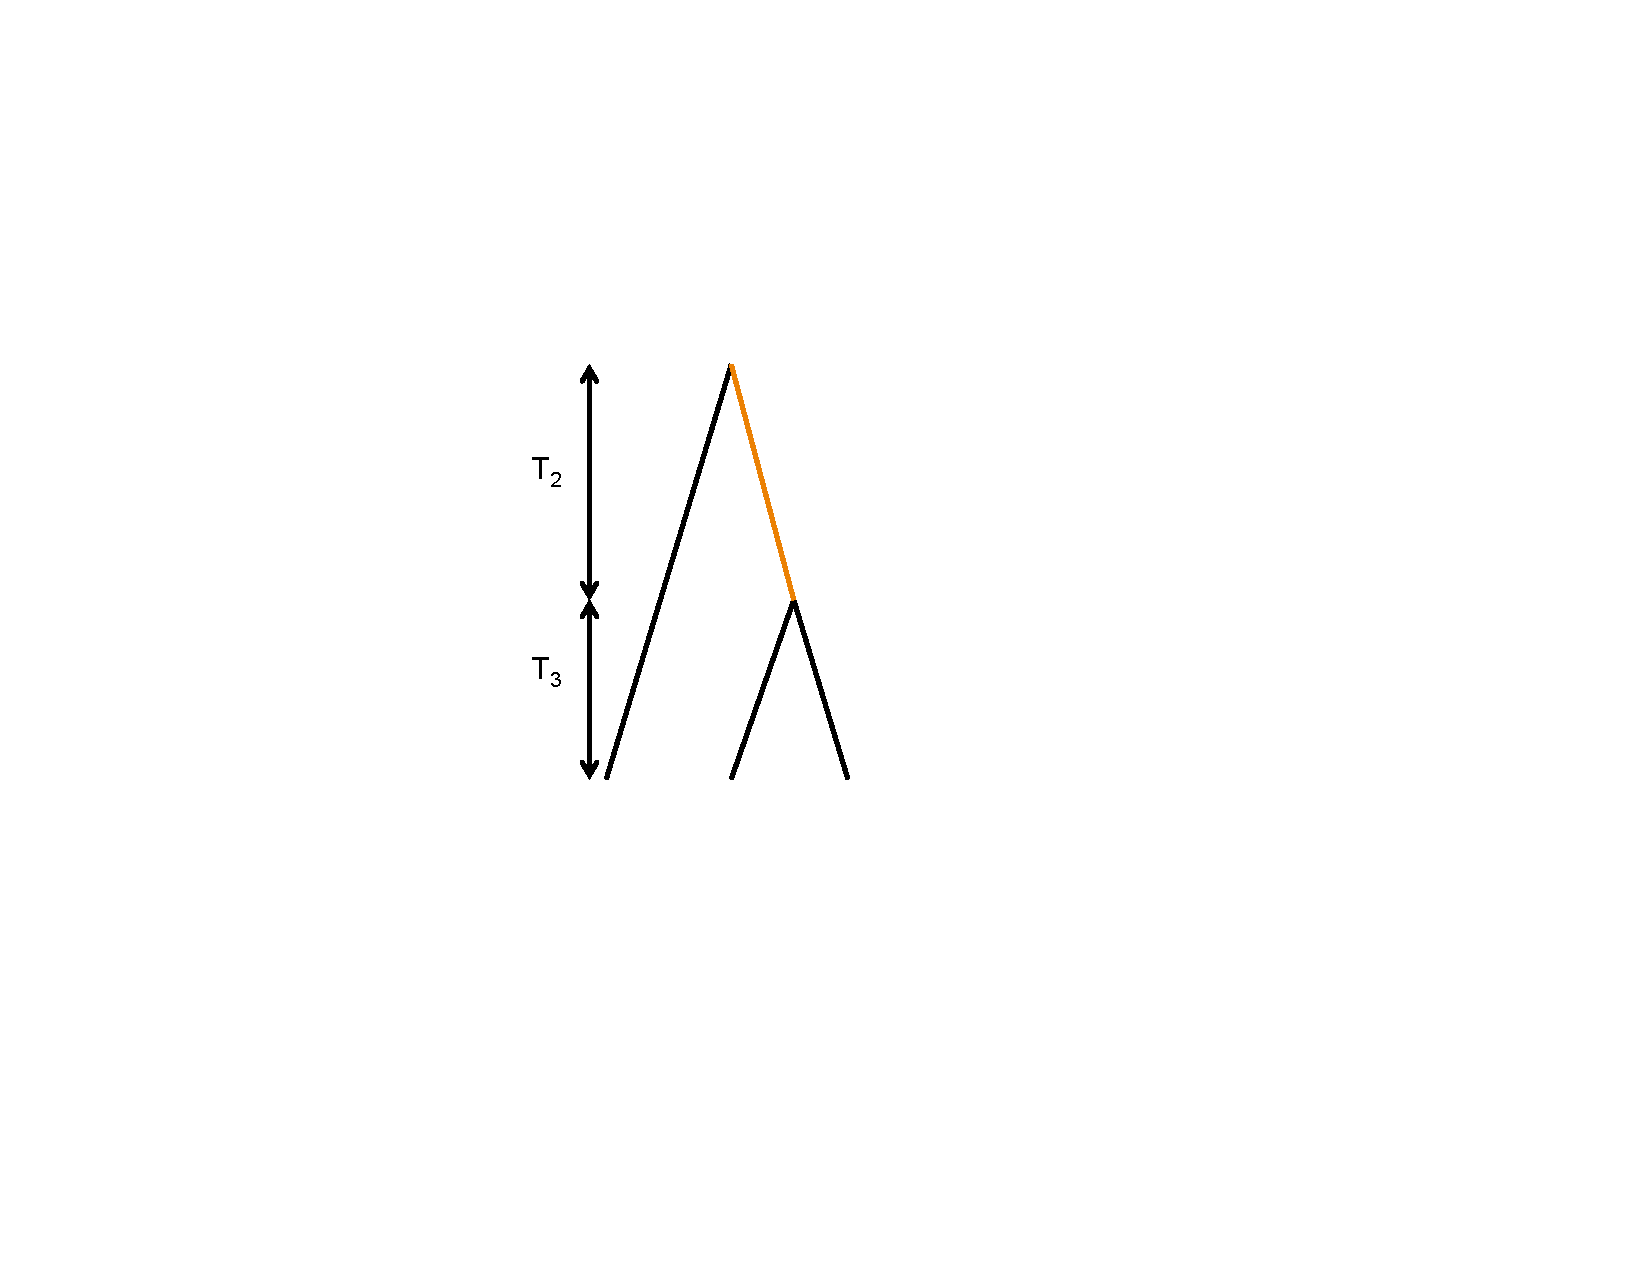
\includegraphics[width= \textwidth]{figures/Genetic_drift/freq_spec_tree.pdf}
\end{center}
\caption{A tree for three samples; note that this is the only possible
tree shape (treating the tips as unlabeled, i.e.  I don't care which pair of sequences carry a doubleton, just that any two sequences carry a derived allele).} \label{fig:freq_coal}
\end{marginfigure}

To see how we could go about working this out, lets start by considering the simple coalescent tree, shown in Figure \ref{fig:freq_coal}, for sample of $3$ alleles drawn from a population. Mutations that fall on the
branches coloured in black will be derived singletons, while mutations that
fall along the orange branch will be doubletons in the sample. The
total number of generations where a singleton mutation could arise is
$3 T_3 + T_2$. Note that we only count the time where there are two
lineages $(T_{2})$ once. So our expected number of singletons, using eqn \eqref{eqn:E_T_i}, is 
\begin{equation}
\E(S_i) = \mu \left( 3\E(T_3) +  \E(T_2) \right) = \mu \left( 3
  \frac{2N}{3}+ 2N \right) = \theta
\end{equation}
By similar logic, the time where doubletons could arise is
$T_2$ and our expected number of doubletons is $\E(S_i)
=\theta/2$. Thus, there are on average half as many doubletons as singletons. 

Extending this logic to larger samples might be doable, but is tedious (I mean really tedious: for 10 alleles there are thousands of possible tree shapes and the task quickly gets impossible even computationally). A nice, relatively simple proof of the neutral site frequency spectrum is given by
\citeauthor{Hudson:15}, but we won't give this here. The general form is: 
\begin{equation}
\E(S_i) = \frac{\theta }{i}   \label{eqn:neutral_freq_spec}
\end{equation}
i.e. there are twice as many singletons as doubletons, three times as many
singletons as tripletons, and so on. The other thing that will be
helpful for us to know is that neutral alleles at intermediate frequency tend to be old, and those that are rare in the sample are young. We expect to see a lot more rare alleles in our sample than common alleles. 

\begin{question}
There are two possible tree shapes that could relate four
samples. Draw both of them and separately colour (or otherwise mark) the branches by where singletons, doubletons, and tripleton derived alleles could arise. 
%{\bf A)} 
%{\bf B)} Can you work out the expected number of each allele count? [{\bf OPTIONAL}] \erin{change for different tree question}
\end{question}

We can also ask the probability of observing a derived allele segregating at frequency $i/n$ given that the site is polymorphic in our sample of size $n$ (i.e. given that $0<i<n$ ). We can obtain this probability by dividing the expected number of sites segregating for an allele at frequency $i$ by the expected number segregating at all of the possible allele frequencies for polymorphisms in our sample 
\begin{eqnarray}
P(i |0<i<n) &=\frac{\E(S_i)}{\sum_{j=1}^{n-1} \E(S_j)} = \frac{\nicefrac{1}{i}}{\sum_{j=1}^{n-1} \nicefrac{1}{j}}.
\end{eqnarray}
We can interpret this probability as the fraction of polymorphic sites we expect to find at a frequency $i/n$. 

\paragraph{tests based on the site frequency spectrum}
Population geneticists have proposed a variety of ways to test whether an observed site frequency spectrum conforms to its
neutral, constant-population expectations. These tests are
useful for detecting population size changes using data across many loci, or
for detecting the signal of selection at individual loci. One of
the first tests was proposed by \citeauthor{tajima:89}, and is called
Tajima's $D$. Tajima's $D$ is
\begin{equation}
  D = \frac{\theta_{\pi}-\theta_{W}}{C} \label{eqn_Tajimas_D}
\end{equation}
where the numerator is the difference between the estimate of
$\theta$ based on pairwise differences and that based on segregating
sites. As these two estimators both have expectation $\theta$ under
the neutral, constant-population model, the expectation of $D$ is zero. The denominator $C$ is a positive constant; it's the square-root of an estimatorof the variance of this difference under the constant population size, neutral model. This constant was chosen for $D$ to have mean zero and variance $1$ under the null model, so we can test for  departures from this simple null model.\\

An excess of rare alleles compared to the constant-population, neutral
model will result in a negative Tajima's $D$, because each
additional rare allele increases the number of segregating sites by
$1$, but only has a small effect on the number of pairwise differences between samples. 
In contrast, a positive Tajima's $D$ reflects an excess of intermediate frequency alleles relative to the constant-population, neutral expectation. Alleles at intermediate-frequency increase pairwise diversity
more per segregating site than typical, thus increasing $\theta_{\pi}$ more than $\theta_{W}$.

\subsection{Demography and the coalescent}

\begin{marginfigure}
\begin{center}
  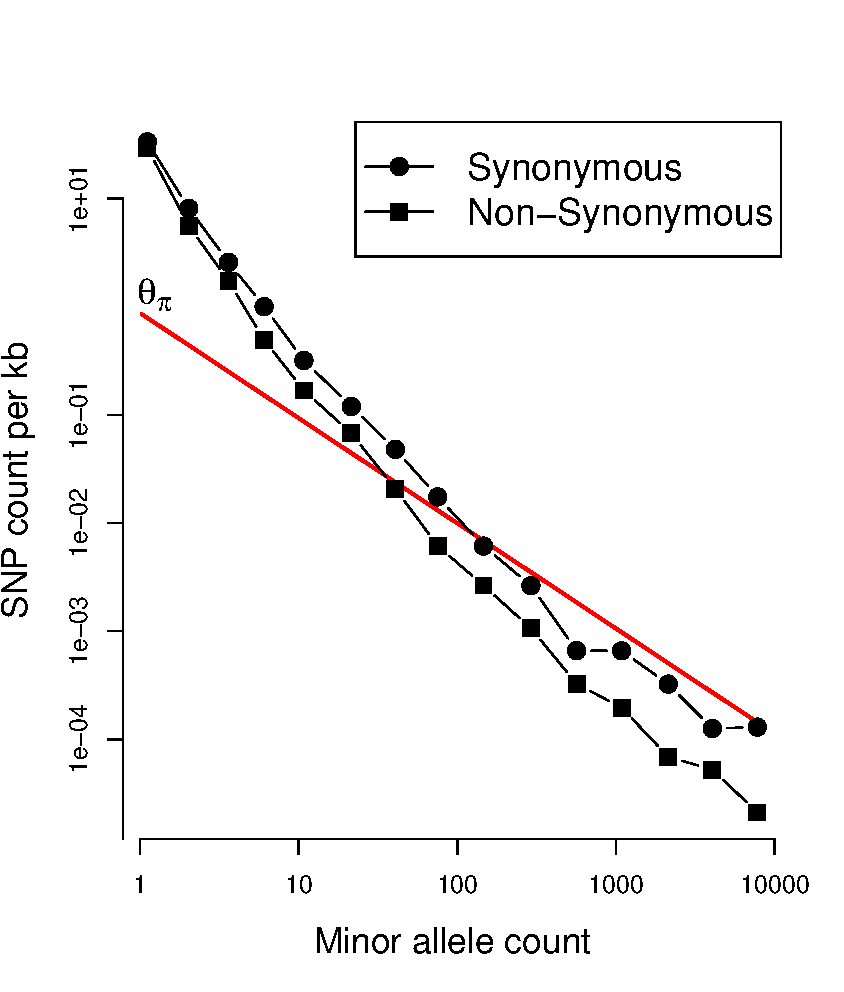
\includegraphics[width = \textwidth]{Journal_figs/genetic_drift/human_pop_growth/Nelson_pop_growth.pdf}
\end{center}
\caption{Data from 202 genes from 14002 people of European ancestry (28004 alleles). Note
  the double log-scale. Redrawn from \citeauthor{nelson:12}. The red
  line gives the neutral, constant population size estimate of the site frequency spectrum, our equation \eqref{eqn:neutral_freq_spec}, using a  $\theta$ estimated from $\pi$. Note how the non-synonymous changes are even more skewed towards rare alleles, that's likely due to selection against non-synonymous alleles acting to push them towards rare frequency.} \label{fig:Human_growth}
\end{marginfigure}
We've already seen how changes in population size can change the rate
at which heterozygosity is lost from the population (see the
discussion around eqn. \eqref{eqn:var_pop_coal}). If the population
size in generation $i$ is $N_i$, the probability that a pair of
lineages coalesce is $\nicefrac{1}{2N_i}$; this conforms to our
intuition that if the population size is small, the rate at which
pairs of lineages find their common ancestor is faster. We can potentially accommodate rapid random fluctuations in population size by simply using the effective population size $N_e$ in place of $N$. However,
longer term more systematic changes in population size will distort
the coalescent genealogies, and hence patterns of diversity, in more
systematic ways. 

We can see how demography potentially distorts the observed frequency spectrum away from the neutral expectation in a very large sample of humans shown in Figure \ref{fig:Human_growth}. For
comparison, the neutral frequency spectrum, eqn
\eqref{eqn:neutral_freq_spec}, is shown as a red line. There are
  vastly more rare alleles than expected under our neutral, constant-population-size model, but the neutral prediction and reality agree somewhat more for alleles that are more common.  

\begin{figure*}
\begin{center}
  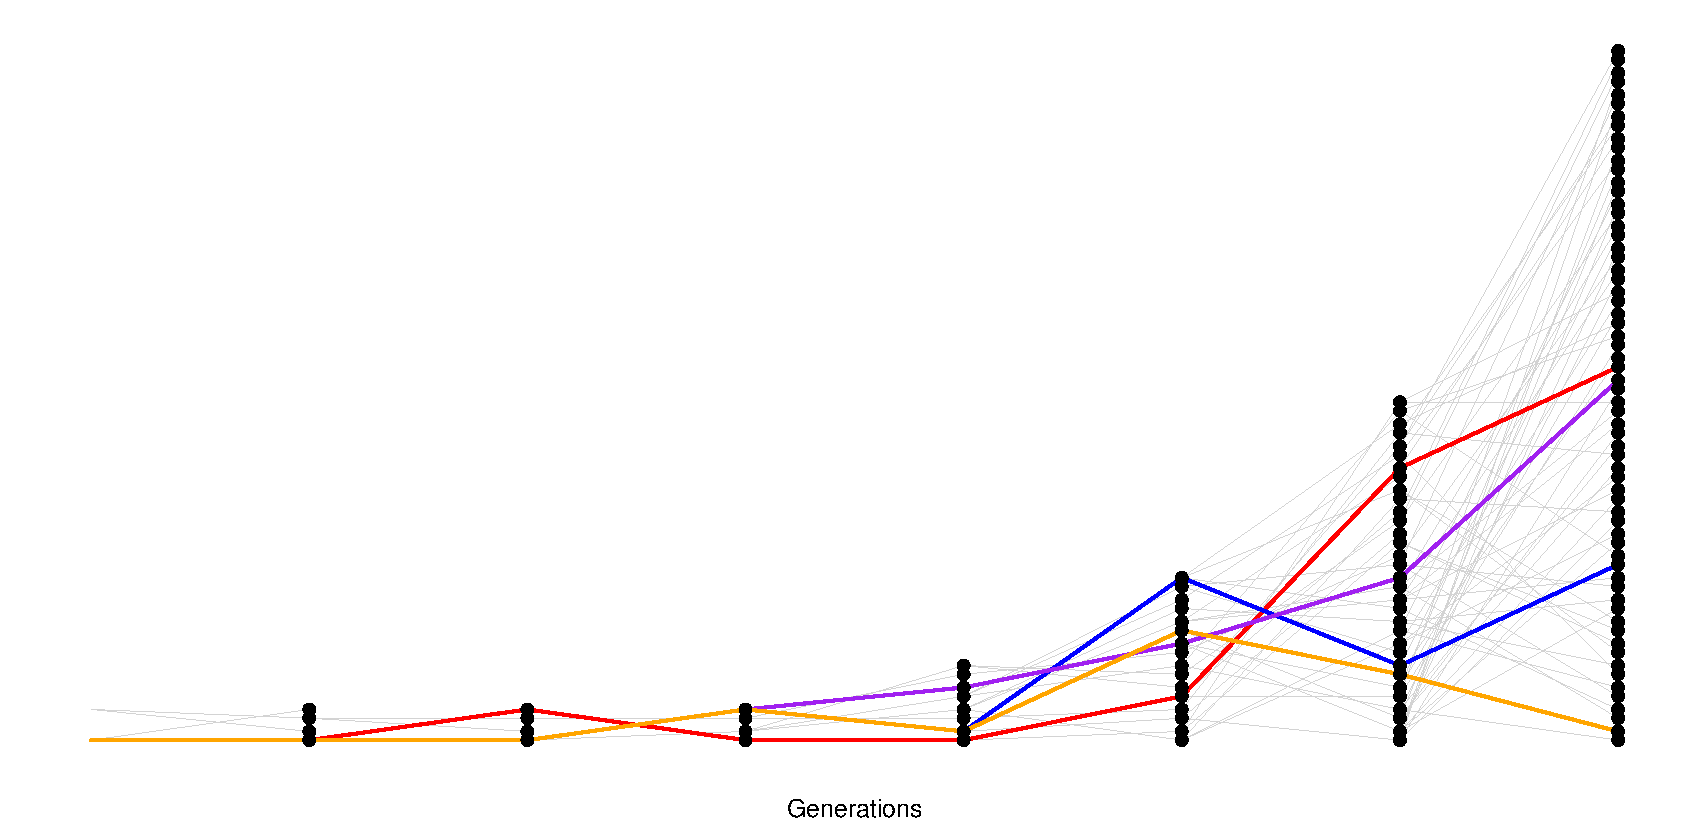
\includegraphics[width = \textwidth]{figures/Genetic_drift/Demography/Growth_genealogy.pdf}
\end{center}
\caption{A realization of the coalescent process in a growing population. The population underwent a period of doubling every generation. The initial population size of just two individuals, maintained for a number of generations, is obviously highly unrealistic but serves our purpose.} \label{fig:Genealogy_growth}
\end{figure*}

Why is this? Well, these patterns are likely the result of the very recent
explosive growth in human populations. If the population has grown rapidly, then the pairwise-coalescent rate in the past may be much higher than the coalescent rate closer to the present. (see Figure \ref{fig:Genealogy_growth}). 

One consequence of a recent population expansion is that there is much less genetic diversity in the population than you'd predict using the census
population size. Humans are one example of this effect; there are $7$ billion
of us alive today, but this is due to very rapid population growth
over the past thousand to tens of thousands of years. Our level of
genetic diversity is very much lower than you'd predict given our
census size, reflecting our much smaller ancestral population. A second consequence of recent population expansion is that the deeper coalescent branches are much more squished together in time, compared to those in a constant population.  Mutations on deeper branches are the source of alleles at more intermediate frequencies, and so there are even fewer intermediate-frequency alleles
in growing populations. That's why there are so many rare alleles,
especially singletons, in this large sample of Europeans. 


Another common demographic scenario is a population bottleneck. In a bottleneck, the population size crashes dramatically, and subsequently
recovers. For example, our population may have had size $N_{\textrm{Big}}$
and crashed down to $N_{\textrm{Small}}$. One example of a
bottleneck is shown in Figure \ref{fig:Genealogy_crash}. 
\begin{figure*}
\begin{center}
  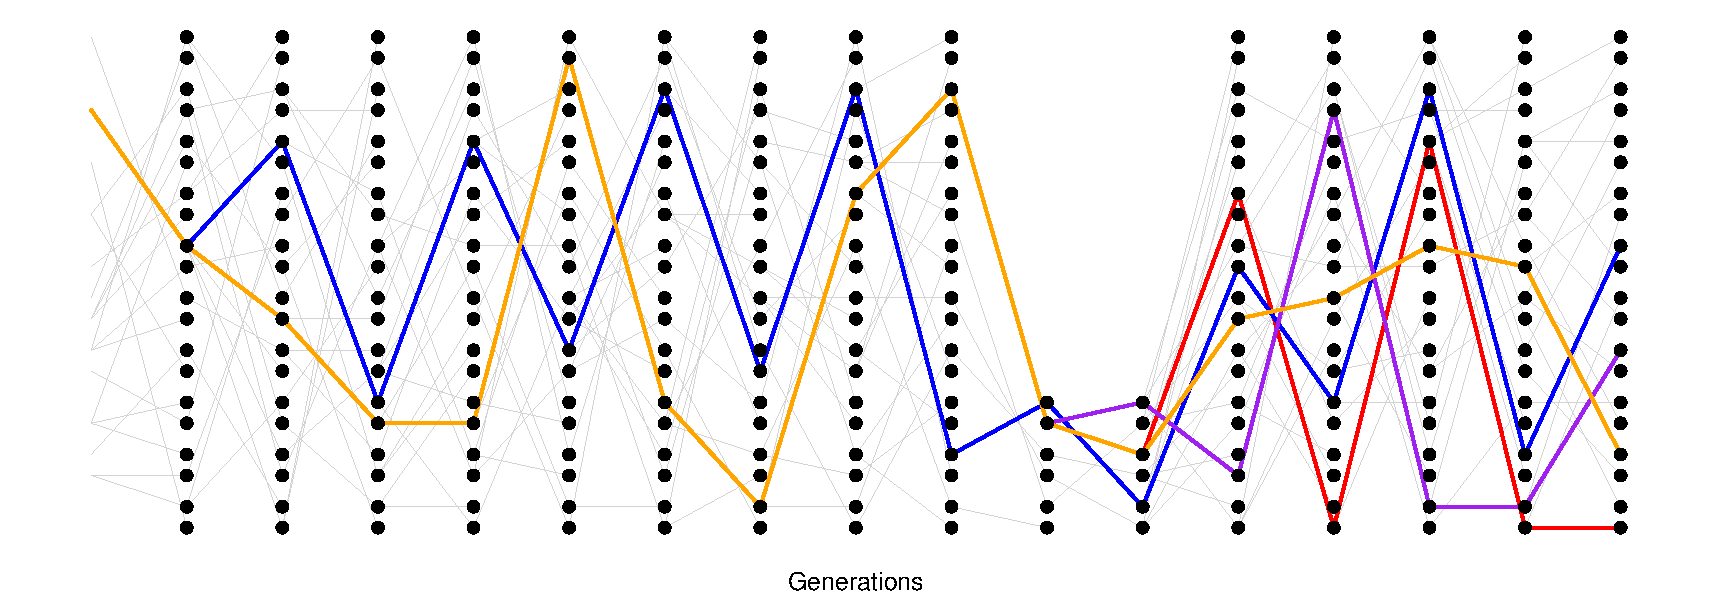
\includegraphics[width = \textwidth]{figures/Genetic_drift/Demography/Crash_genealogy.pdf}
\end{center}
\caption{A realization of the coalescent process in a bottlenecked population. Our population under went a bottleneck eight generations in the past.} \label{fig:Genealogy_crash}
\end{figure*}
Looking at a sample of lineages drawn from the population today, if
the bottleneck was somewhat recent ($\ll N_{\textrm{Big}}$ generations
in the past) many of our lineages will not have coalesced before reaching
the bottleneck, moving backward in time. But during the bottleneck our
lineages coalesce at a much higher rate, such that many of our
lineages will coalesce if the bottleneck lasts long enough
($\sim N_{\textrm{Small}}$ generations). If the bottleneck is very
strong, then all of our lineages will coalesce during the bottleneck, and the resulting site frequency spectrum may
look very much like our population growth model (i.e. an excess of rare
alleles). However, if some pairs of lineages escape coalescing during
the bottleneck, they will coalesce much more deeply in time (e.g. the
blue and orange ancestral lineages in
\ref{fig:Genealogy_crash}). 
\begin{figure}
\begin{center}
  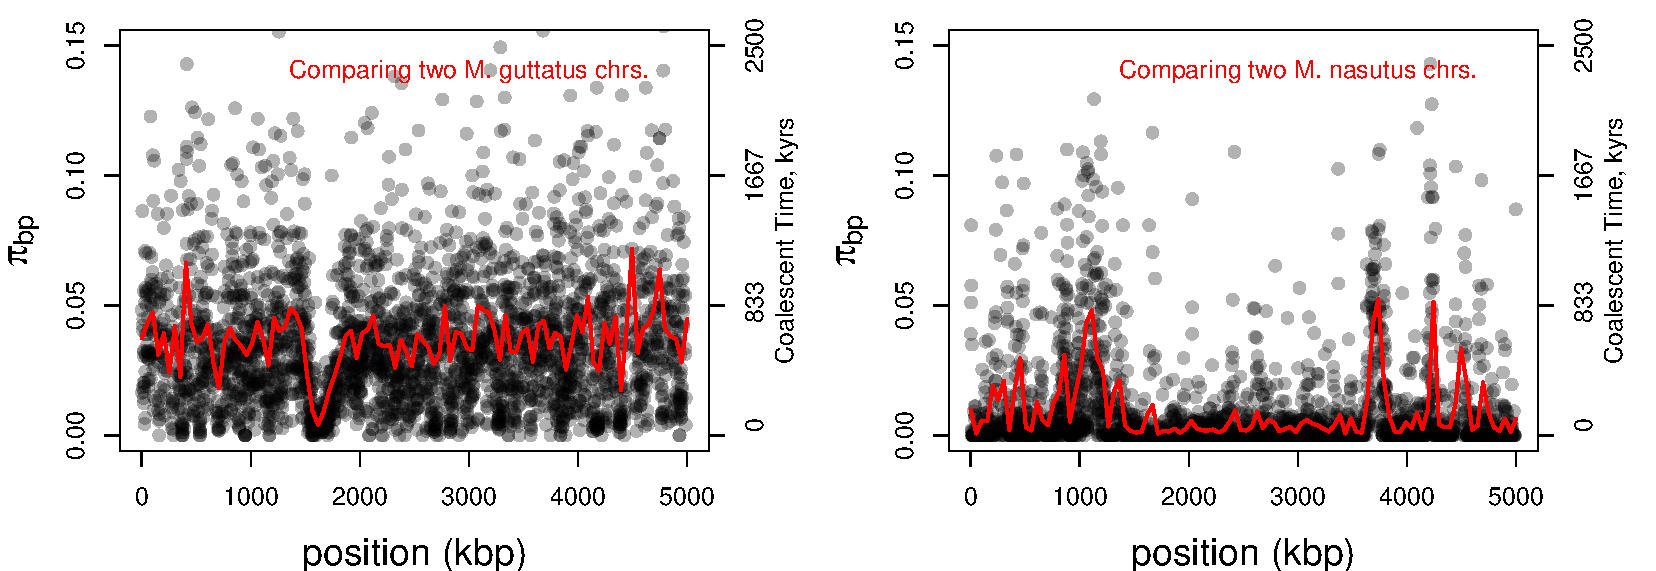
\includegraphics[width = \textwidth]{figures/Genetic_drift/Demography/Mimulus_coalescent_times.pdf}
\end{center}
\caption[][-2cm]{Diversity along the Mimulus genome. Black dots give $\pi$ in 1kb windows between chromosomes sampled from two individuals, the red line is a
  moving average (data from  \citeauthor{brandvain:14}). Pairwise coalescent times ($t$) estimated assuming $t= \nicefrac{\pi}{2 \mu} $ using $\mu_{BP}=10^{-9}$.} \label{fig:Mimulus_bottleneck}
\end{figure}
\begin{marginfigure}[2cm]
\begin{center}
  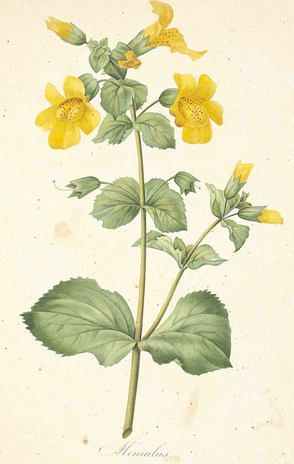
\includegraphics[width = 0.75 \textwidth]{illustration_images/Genetic_drift/Mimulus/Mimulus.png}
\end{center}
\caption{{\it M. guttatus} by Pierre-Joseph
  Redout\'e.} \label{fig:Human_growth}  %é
\end{marginfigure}
An example of this is shown Figure
\ref{fig:Mimulus_bottleneck}, data from \citeauthor{brandvain:14}. {\it Mimulus nasutus} is a selfing
species that arose recently from an out-crossing progenitor {\it M.
  guttatus}, and experienced a strong bottleneck. {\it M. guttatus} has a very high levels of genetic diversity
($\pi=4\%$ at synonymous sites), but {\it M. nasutus} has lost much 
of this diversity ($\pi =1\%$). Looking along the genome, between a
pair of {\it M. guttatus} chromosomes, levels of
diversity are fairly uniformly high.

 But in comparing two {\it
  M. nasutus} chromosomes, diversity is low because the pair of lineages generally coalesce
recently. Yet in a few places we see levels of diversity comparable to
{\it M. guttatus}; these regions correspond to genomic sites where our pair of lineages
fail to coalesce during the bottleneck and subsequently coalesce
much more deeply in the ancestral {\it M. guttatus} population.
\begin{figure}
\begin{center}
  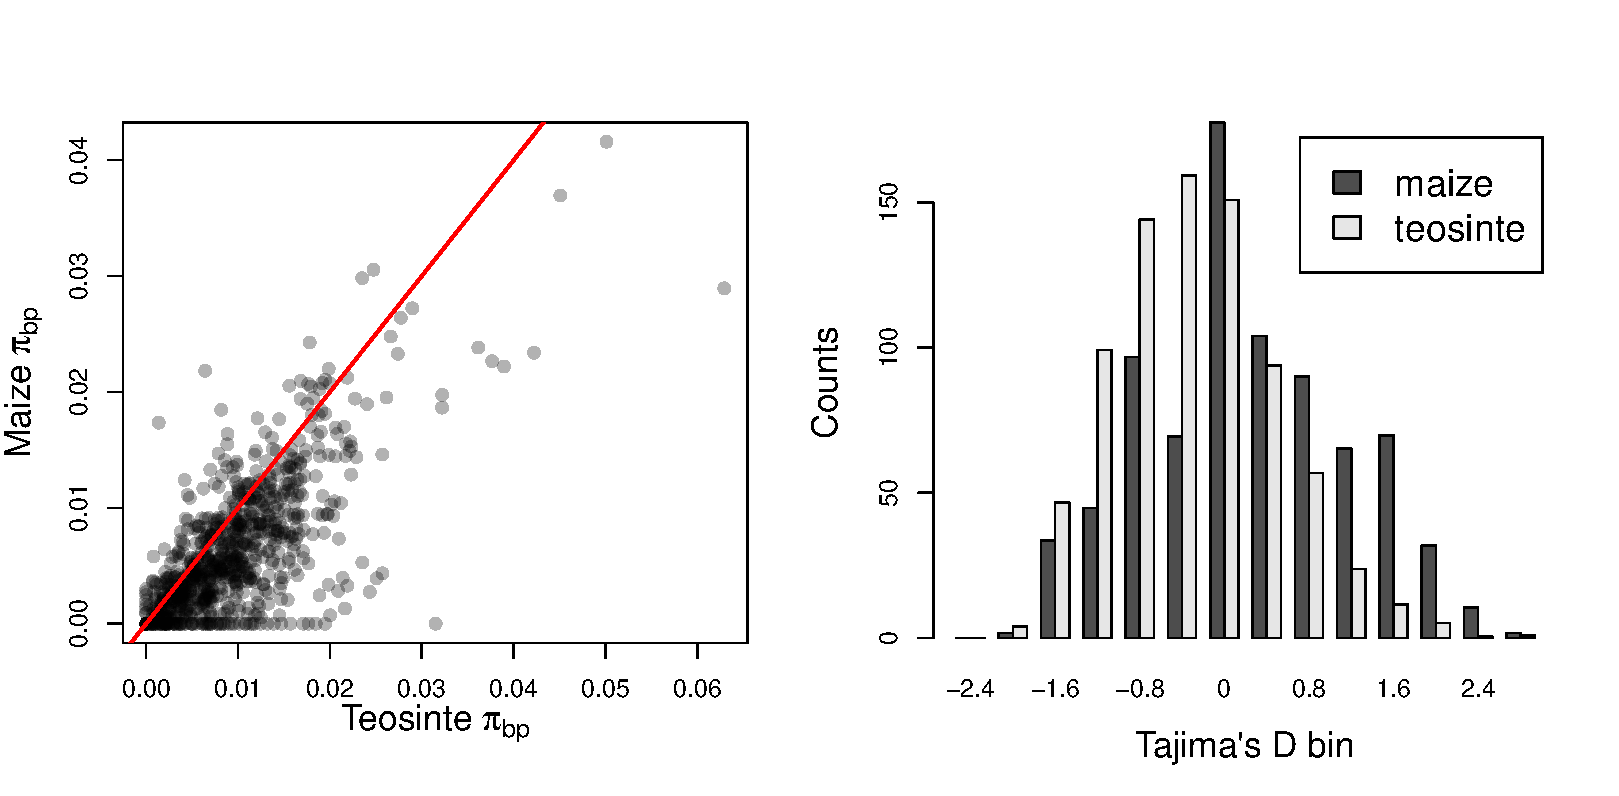
\includegraphics[width = \textwidth]{Journal_figs/genetic_drift/Maize_bottleneck/Wright_Tajima_D.pdf}
\end{center}
\caption[][-2cm]{Data for polymorphism from Maize and Teosinite: 774
  genes redrawn from \citet{Wright:05}. {\bf Left)} Genetic  diversity levels in maize and and Teosinte samples at each of these genes.
Note how diversity levels are lower in maize than teosinte, i.e. most
points are below the red $x=y$ line.  
. {\bf Right)} The distribution of Tajima's D in maize and teosinte, see how the maize distribution is shifted towards positive values. } \label{fig:maize_Tajimas_D}  %é
\end{figure}
\begin{marginfigure}[4cm]
\begin{center}
  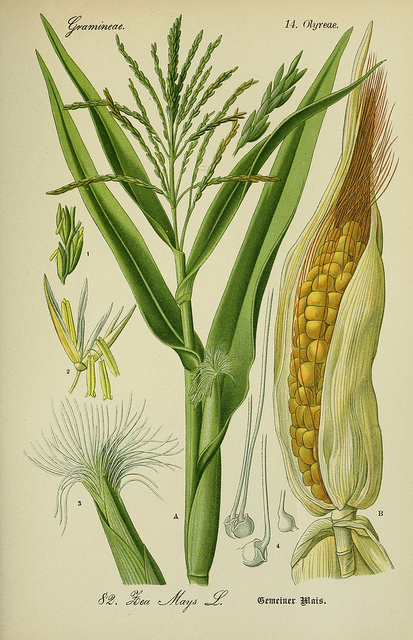
\includegraphics[width = \textwidth]{illustration_images/Genetic_drift/maize/7845339168_66aa3d8ccc_z.jpg}
\end{center}
\caption{Maize ({\it Zea mays}.) Prof. Dr. Thomé's Flora von
  Deutschland. 1886. Thomé, O. W. } \label{fig:maize}  %é
\end{marginfigure}  %%possible different fig https://peerj.com/preprints/26502.pdf from Jeff's paper

Mutations that arise on deeper lineages will be at intermediate frequency in our sample, and so mild bottlenecks
can lead to an excess of intermediate frequency alleles compared to
the standard constant-population model. This can skew 
Tajima's D, see eqn \ref{eqn_Tajimas_D}, towards positive values and away from its expectation of
zero . One example of this skew is shown in Figure
\ref{fig:maize_Tajimas_D}. Maize ({\it (Zea mays} subsp.{\it mays}) was domesticated from its wild progenitor teosinte ({\it (Zea mays
subsp. parviglumis}) roughly ten thousand years ago. We can see how the
 bottleneck associated with domestication has resulted in a loss of genetic diversity in maize, compared to teosinte, and the polymorphism that remains is somewhat skewed towards intermediate frequencies resulting in more positive values of Tajima's D.

\begin{question}
\citet{voight2005interrogating} sequenced 40 autosomal regions from 15 diploid samples of Hausa people from Yaounde, Cameroon. The average length of locus they sequenced for each region was $2365$bp. They found that the average number of segregating sites per locus was $S= 11.1$ and the average $\pi = 0.0011$ per base over the loci. Is Tajima's D positive or negative? 
\end{question}








\section{Molecular Evolution and the fixation of neutral alleles} 
\begin{quote}
"history is just one damn thing after another" -Arnold Toynbee 
\end{quote} %https://quoteinvestigator.com/2015/09/16/history/

It is very unlikely that a rare
neutral allele accidentally drifts up to fixation; more likely, such an allele
will be eventually lost from the population. However, populations experience a
large and constant influx of rare alleles due to mutation, so even if it is
very unlikely that an individual allele fixes within the population, some
neutral alleles will fix by chance. \\


%We'll first consider the probability that a neutral allele fixes
%within the population, starting from it just enters a diploid
%population as a newly mutated allele at frequency $1/(2N)$.

%so for an allele to be fixed in the population it
%must have been that allele

\paragraph{Probability of the eventual fixation of a neutral allele}
% TODO: tried to clean up this section, needs more work
\begin{figure}
\begin{center}
  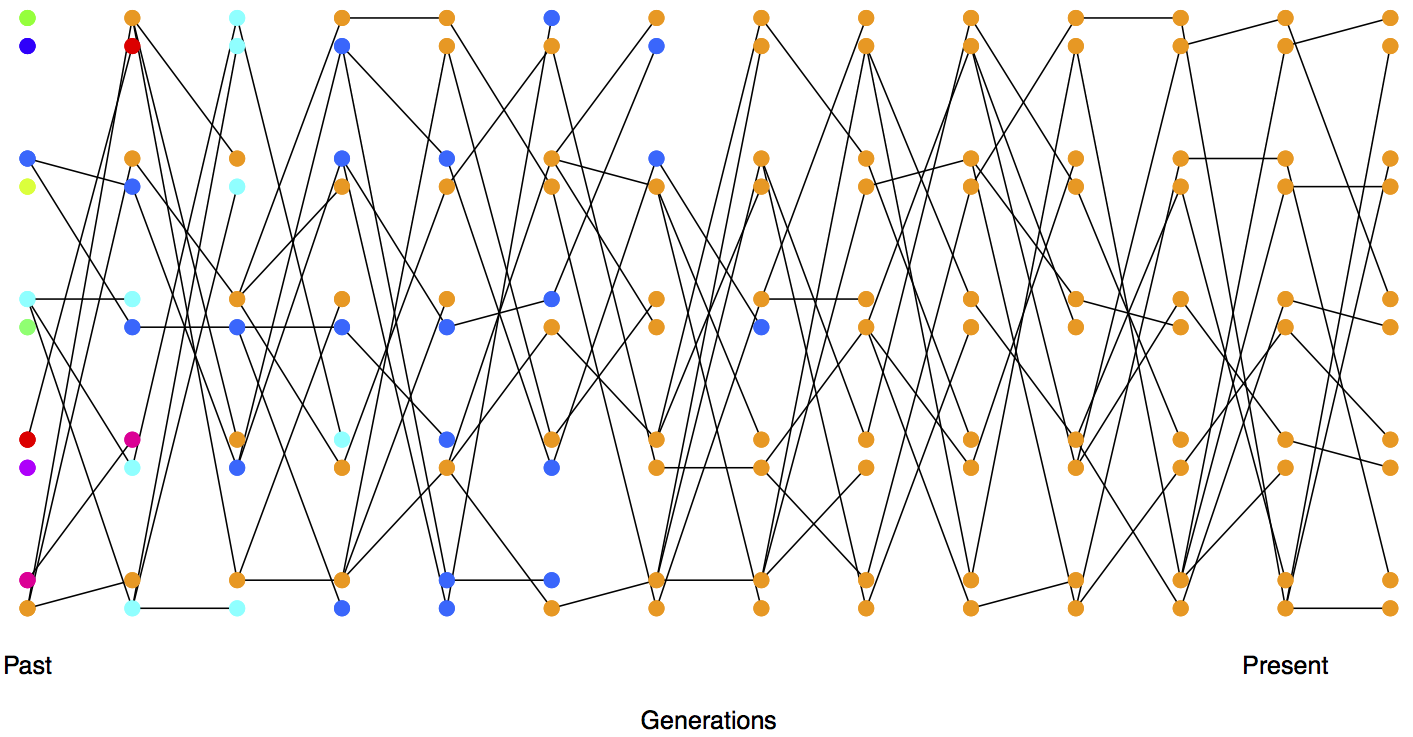
\includegraphics[width = \textwidth]{figures/Substitution_sim.png}
\end{center}
\caption{Each allele initially present in a small diploid population is
  given a different colour so we can track their descendants over
  time. By the 9th generation, all of the alleles present in the
  population can trace their ancestry back to the orange allele.} \label{fig:subs_simulation}
\end{figure}

An allele which reaches fixation within a population is an ancestor to the
entire population. In a particular generation there can only be a single allele
that all other alleles at the locus in a later generation can claim as an
ancestor (See Figure \ref{fig:subs_simulation}). At a neutral locus, the actual allele does not affect the number of
descendants that the allele has (this follows from the definition of
neutrality: neutral alleles don't leave more or less descendants on average than other neutral alleles).
An equivalent way to state this is that the allele labels don't affect
anything; thus the alleles are \emph{exchangeable}. As a consequence of being exchangeable,
any allele is equally likely to be the ancestor of the entire population.  In a
diploid population of size $N$, there are $2N$ alleles, all of which are
equally likely to be the ancestor of the entire population at some later time
point. So if our allele is present in a single copy, the chance that it is the
ancestor to the entire population in some future generation is
$\nicefrac{1}{(2N)}$, i.e. the chance our neutral allele is eventually fixed is
$\nicefrac{1}{(2N)}$.  In Figure \ref{fig:subs_simulation}, our orange allele
in the first generation is one of 10 differently coloured alleles, and so has a
$1/10$ chance of being the ancestor of the entire population at some later time
point (and in this simulation it does become the common ancestor, by the 9th generation).\\

More generally, if our neutral allele is present in $i$ copies in the
population, of $2N$ alleles, the probability that this allele becomes fixed is
$\nicefrac{i}{(2N)}$, i.e. the probability that a neutral allele is eventually
fixed is simply given by its frequency ($p$) in the population.  (We can also
derive this result by letting $Ns \rightarrow 0$ in eqn.
\eqref{eqn:prob_fixed}, a result we'll encounter later.)




% TODO
A newly arisen mutation only becomes a fixed difference if it is lucky
enough to be the ancestor of the entire population. As we saw above, this occurs
with probability $\nicefrac{1}{(2N)}$. 

How long does it take on average for
such an allele to fix within our population? Well, in developing
equation \eqref{TMRCA_neutral} we've seen that it takes $4N$
generations for a large sample of alleles to all trace their ancestry back to a
single most recent common ancestral allele. Any single-base pair change which arose as a single mutation at a locus, and fixed in the population, must have been present in the sequence transmitted by the most recent common ancestor of the population at that locus. Thus it must take roughly $4N$ generations
for a neutral allele present in a single copy within the population to the
ancestor of all alleles within our population.  This argument can be made more
precise, but in general we would still find that it takes $\approx 4N$
generations for a neutral allele to go from its introduction to fixation with
the population.   \\

\paragraph{Rate of substitution of neutral alleles}

A substitution between populations that do not exchange gene flow is simply a
fixation event within one population. The rate of substitution is therefore the
rate at which new alleles fix in the population, so that the long-term
substitution rate is the rate at which mutations arise that will eventually
become fixed within our population.\\

Lets assume, based on our discussion of the neutral theory of molecular evolution, that there are only two classes of mutational changes that can occur with a
region, highly deleterious mutations and neutral mutations. A fraction $C$ of
all mutational changes are highly deleterious, and cannot possibly contribute
to substitution nor polymorphism.  The other $1-C$ fraction
of mutations are neutral. If our mutation rate is $\mu$ per transmitted allele
per generation, then a total of $2N \mu (1-C)$ neutral mutations enter our
population each generation.\\

Each of these neutral mutations has a $\nicefrac{1}{(2N)}$ probability chance of
eventually becoming fixed in the population. Therefore, the rate at
which neutral mutations arise that eventually become fixed within our
population is  
\begin{equation}
2N\mu(1-C)\frac{1}{2N} = \mu(1-C)
\end{equation}
Thus the rate of substitution, under a model where newly arising alleles are either
highly deleterious or neutral, is simply given by the mutation rate
of neutral alleles, i.e. $\mu(1-C)$.\\

Consider a pair of species that have diverged for $T$ generations, i.e. orthologous sequences shared between the species last shared a common ancestor $T$ generations ago. If these species have maintained a constant $\mu$ over that time, they will have accumulated an average of
\begin{equation}
2\mu(1-C)T \label{eqn:moleclock}
\end{equation}
neutral substitutions. This assumes that $T$ is a lot longer than the time it
takes to fix a neutral allele, such that the total number of 
alleles introduced into the population that will eventually fix is the
total number of substitutions.\\

This is a really pretty result as the population size has completely canceled
out of the neutral substitution rate. However, there is another way to see this
in a more straight forward way. If I look at a sequence in me compared to, say, a
particular chimp, I'm looking at the mutations that have occurred in both of
our germlines since they parted ways $T$ generations ago. Since neutral alleles
do not alter the probability of their transmission to the next generation, we
are simply looking at the mutations that have occurred in $2T$ generations
worth of transmissions. Thus the average number of neutral mutational
differences separating our pair of species is simply $2\mu (1-C) T$.\\

\marginnote{\begin{quote}"functionally less important molecules or parts of a molecule
evolve faster than more important ones." \end{quote} -- \citet{kimura1974some}}
A number of observations follow under this model, from equation \eqref{eqn:moleclock}, the first is that a primary determinant of patterns of molecular evolution in a genomic region is the level of constraint ($C$). This pattern generally seems to hold empirically: non-coding regions often evolve more rapidly than coding regions; synonymous substitutions accumulate faster than nonsynonymous; nonsynonymous changes faster in less vital proteins than ones that are absolutely necessary for early development. Note that this is not a unique prediction of the neutral model, e.g. lower pleiotropy means that less constrained regions may be better able to evolve adaptively. However, it is a fantastically useful general insight, e.g. it allows us to spot putatively functional non-coding regions by looking for genomic regions that have very low levels of divergence among distantly related species.

\begin{figure}
\begin{center}
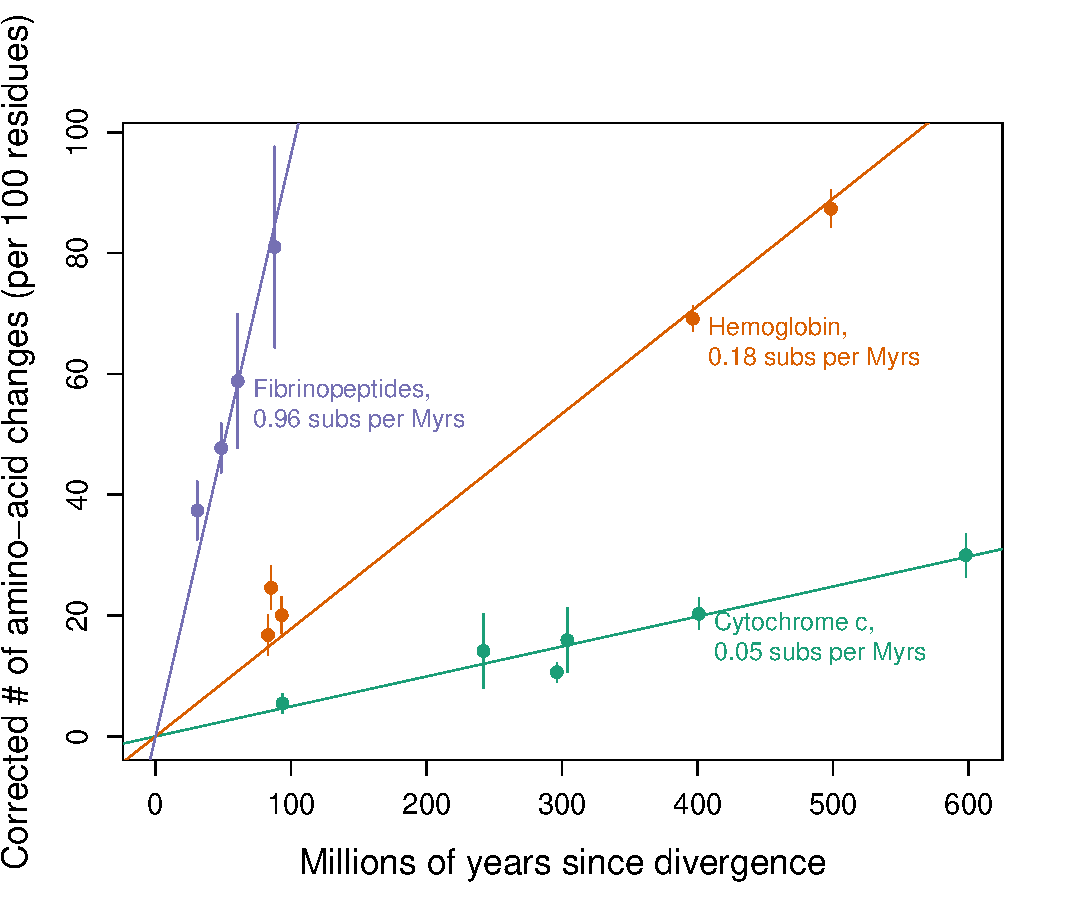
\includegraphics[width=0.8 \textwidth]{Journal_figs/genetic_drift/Molecular_clock_Dickerson/Dickerson_1979_mole_clock_fig.pdf}
\end{center}
\caption{The numbers of substitutions between various pairs of groups, for three proteins, plotted against the time these groups shared a common ancestor in the fossil record. Data from  \citet{dickerson1971structure}. The number of observed amino-acid differences is corrected for multiple hits to obtain the corrected number of changes estimated to occur. The lines give the linear regression, constrained to pass through the origin, for each protein. The slope of the regression is given next to the protein name. } \label{fig:Dickerson_mole_clock}  
\end{figure}


The second important insight, and critical for the development of the neutral theory, is that equation \eqref{eqn:moleclock} is seemingly consistent with \citet{zuckerkandl1965evolutionary}'s hypothesis of a surprisingly constant, protein molecular clock. See Figure \ref{fig:Dickerson_mole_clock} for an example using the data of \citet{dickerson1971structure}. If we double the amount of time separating a pair of species $T$, we double the number of substitutions predicted. Note that for this to be true $T$ must be measured in generations. To explain a protein molecular clock between species that clearly differed dramatically in generation time it was hypothesized that the mutation rate actually scaled with generation time, i.e. short-lived organisms introduced less mutations per generation, e.g. as they had fewer rounds of mitosis. This generation-time assumption meant that the mutation rate per year could be constant, such that $\mu T$ would be a constant for pairs of species that had diverged for similar geological times, which are measured in years, even if the organisms differed in generation time. This assumption would allow neutral theory to be consistent with a protein molecular clock measured in years. We now know that this critical generation time assumption is false, organisms with shorter generation times have somewhat higher mutation rates per year, and so a strict neutral model is inconsistent with the protein molecular clock. We'll return to these ideas when we discuss the fate of very weakly selected mutations in Chapter \ref{Selection_Stochasticity} and \citet{ohta1973slightly}'s Nearly Neutral theory. If you are still reading this send Graham a picture of Tomoko Ohta receiving the Crafoord Prize, an analog of the Nobel prize for biology, for her contributions to molecular evolution. 




\begin{marginfigure}
\begin{center}
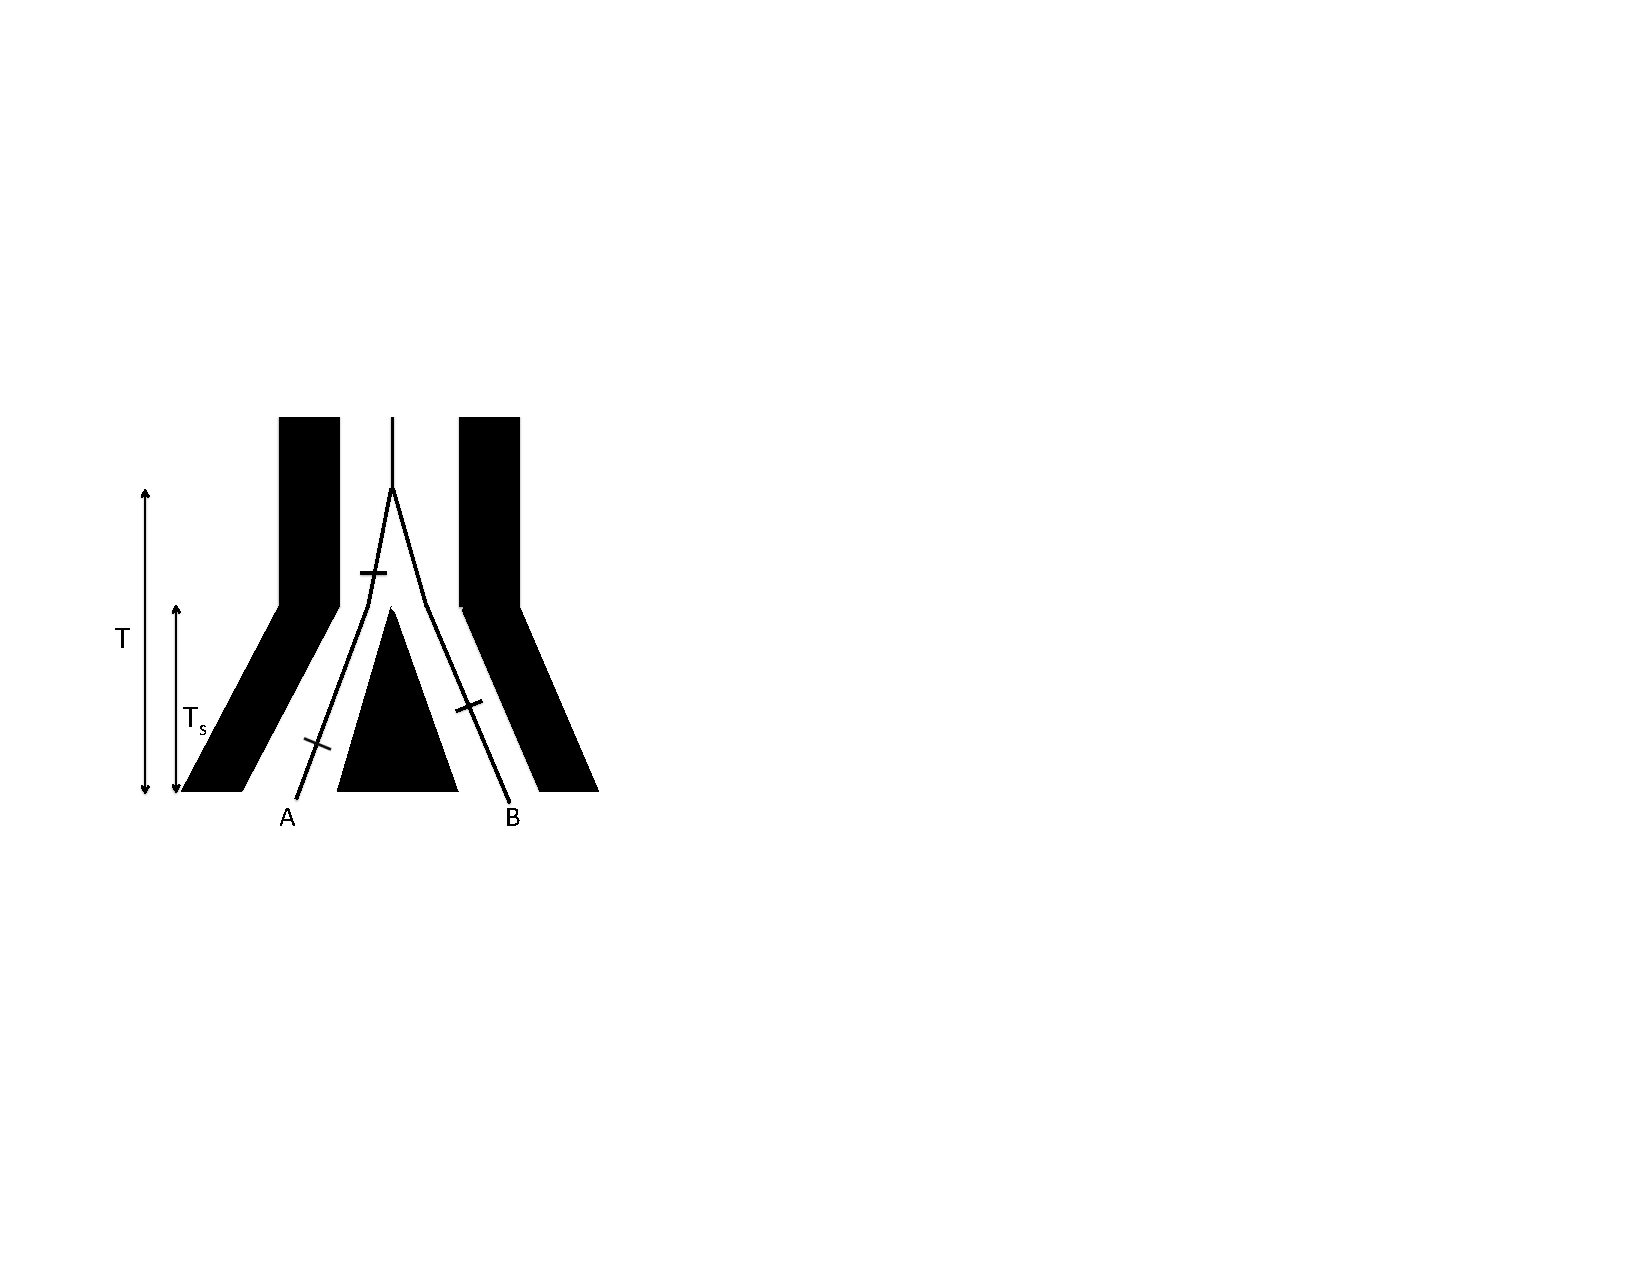
\includegraphics[width=0.8 \textwidth]{figures/Genetic_drift/ILS/split_anc_pop.pdf}
\end{center}
\caption{The genealogy of two alleles one sampled from population A and B. Mutations on the lineages are shown as dashes. The pair of alleles coalesce in the ancestral population of A and B. The two populations split $T_S$ generations ago, with no subsequent gene flow, but the two lineages must coalesce deeper in time. } \label{fig:split_anc_pop}  
\end{marginfigure} 


\paragraph{The contribution of ancestral polymorphism to divergence.} If we are considering $T$ to represent the divergence between long-separated species, then we can think of $T$ as the time that the
species split. However, for more recently diverged populations and
species, we need to include the fact that the sorting of ancestral
polymorphism contributes to divergence among species. In Figure 
\ref{fig:split_anc_pop}, we see our two populations split $T_s$ generations ago.  However, the
coalescence of our A and B lineage is necessarily deeper in time than
$T_s$. The top mutation was polymorphic in the ancestral population
but now contributes to the divergence between A and B. Assuming that
our ancestral population had effective size $N_A$ individuals, and
that our populations split cleanly with no subsequent gene flow, then
\begin{equation}
T = T_s + 2N_A.
\end{equation}
If our species split time is very large compared to $2N$ then we can think of $T$ as the split time. 

%Our expected number of substitutions is scaling linearly with our species $T$ split time measured in generations.  

%\erin{I think this last concept is hard and may be a bit confusing for students without some additional pictures or text} %\graham{lineup split time in this section w. FST section.}



\begin{question}
For this, and the next question, assume that humans and chimp diverged
%\graham{Update numbers?}
around 5.5$\times 10^6$ years ago, have a generation time ~20 years, that the speciation occurred instantaneously in allopatry with no subsequent gene flow, and the ancestral effective population size of the human and chimp common ancestor population was 10,000 individuals.\\
Nachman and Crowell sequenced 12 pseudogenes in human and chimp and found substitutions at 1.3\% of sites. \\
{\bf A) } What is the mutation rate per site per generation at these genes?\\
{\bf B)} All of the pseudogenes they sequenced are on the autosomes. What
would your prediction be for pseudogenes on the X and Y chromosomes,
given that there are fewer rounds of replication in the female
germline than in the male germline.
\end{question}

\section{Tests of molecular evolution.}

\subsection{Comparing the rates of non-synonymous to synonymous
substitutions $\dNdS$}
A common test molecular evolution is to compare the ratio of the rates of non-synonymous to synonymous
substitutions. The simplest way to calculate $d_N$ is to 
count up the non-synonymous changes and divide by the total number of
positions in the gene where a non-synonymous change could occur. We
can do likewise for $d_S$, and then take the ratio. This is a helpful
conceptual way to think about what $\dNdS$ represents, however, this
ignores the fact that particular changes are more likely to occur by
mutation and also does not account for multiple hits. Therefore, in
practice $\dNdS$ is more usually calculated by model-based
likelihood and bayesian methods
that can account for these features (see \gc{XX}). 

For the vast majority of genes in the genome we see that $\dNdS < 1$, this is consistent with the view
that non-synonymous sites are much more constrained than synonymous, i.e. that most non-synonymous mutations are deleterious and quickly
removed from the population. If we are willing to make the assumption that all synonymous changes are
neutral, $d_S=2T \mu$, then we can estimate the degree of constraint. (Note that synonymous changes can sometimes be subject to
both positive and negative selection, but we have to start somewhere.) 

Assuming that a fraction $C$ of non-synonymous changes are too
deleterious to contribute to polymorphism then, if $T$ generations of divergence have
elapsed between the two populations we expect
\begin{equation}
d_N = 2T (1-C) \mu  
\end{equation}
Then
\begin{equation} 
\dNdS = (1-C) 
\end{equation}
therefore, if we assume that non-synonymous mutations can only be
strongly deleterious or neutral, we estimate the fraction of mutational changes that
are constrained by negative selection as $C= 1- \dNdS$. This has the
interpretations of being the fraction of non-synonymous mutations that are quickly weeded out of the population by selection, and so do not contribute to divergence among species. 

\paragraph{Loss of constraint at pseudogenes.}

\begin{marginfigure}
\begin{center}
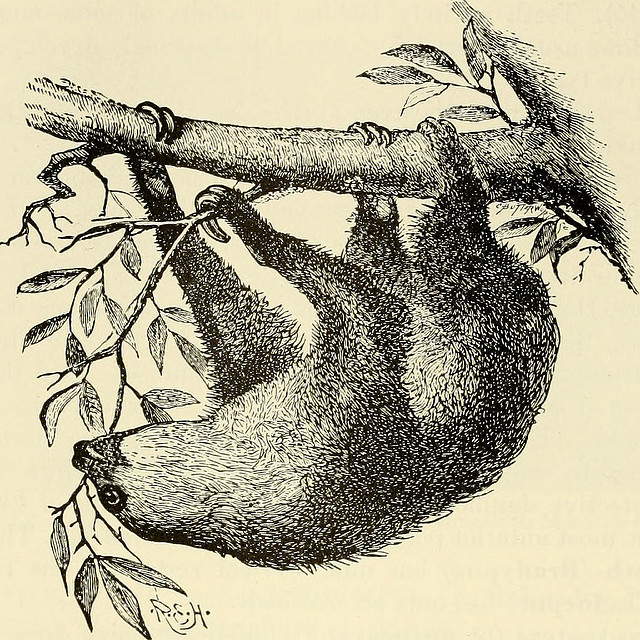
\includegraphics[width=\textwidth]{illustration_images/Genetic_drift/sloth/20423856040_6e4360df9c_z.jpg}
\end{center}
\caption{Two-toed sloth ({\it Choloepus hoffmanni}). An introduction
  to the study of mammals, living and extinct. 1891. Flower W. H. and Lydekker R.} \label{fig:sloth}  
\end{marginfigure} 

While most genes evolve under constraint, we can find examples of
genes that are evolving in a less constrained manner. The simplest
example of this is where the gene has lost function, e.g. has recently
become pseudogenized. When a gene completely loses function there will be no
selection against non-synoynous changes and so they are just as free
to accumulate as synonymous changes, and so $\dNdS=1$.
Genes can lose function because of inactivating mutations that stop
them being transcribed or translated into functional proteins, such genes are
called pseudogenes. Our genomes are filled with old pseudogenes whose
meaning are slowly being eroded through the accumulation of neutral substitutions.
One nice example of as gene that has been repeatedly lost function,
i.e. become repeatedly psuedogenized, is
the Enamlin gene from the study of \citeauthor{Meredith:09}.

\begin{figure}
\begin{center}
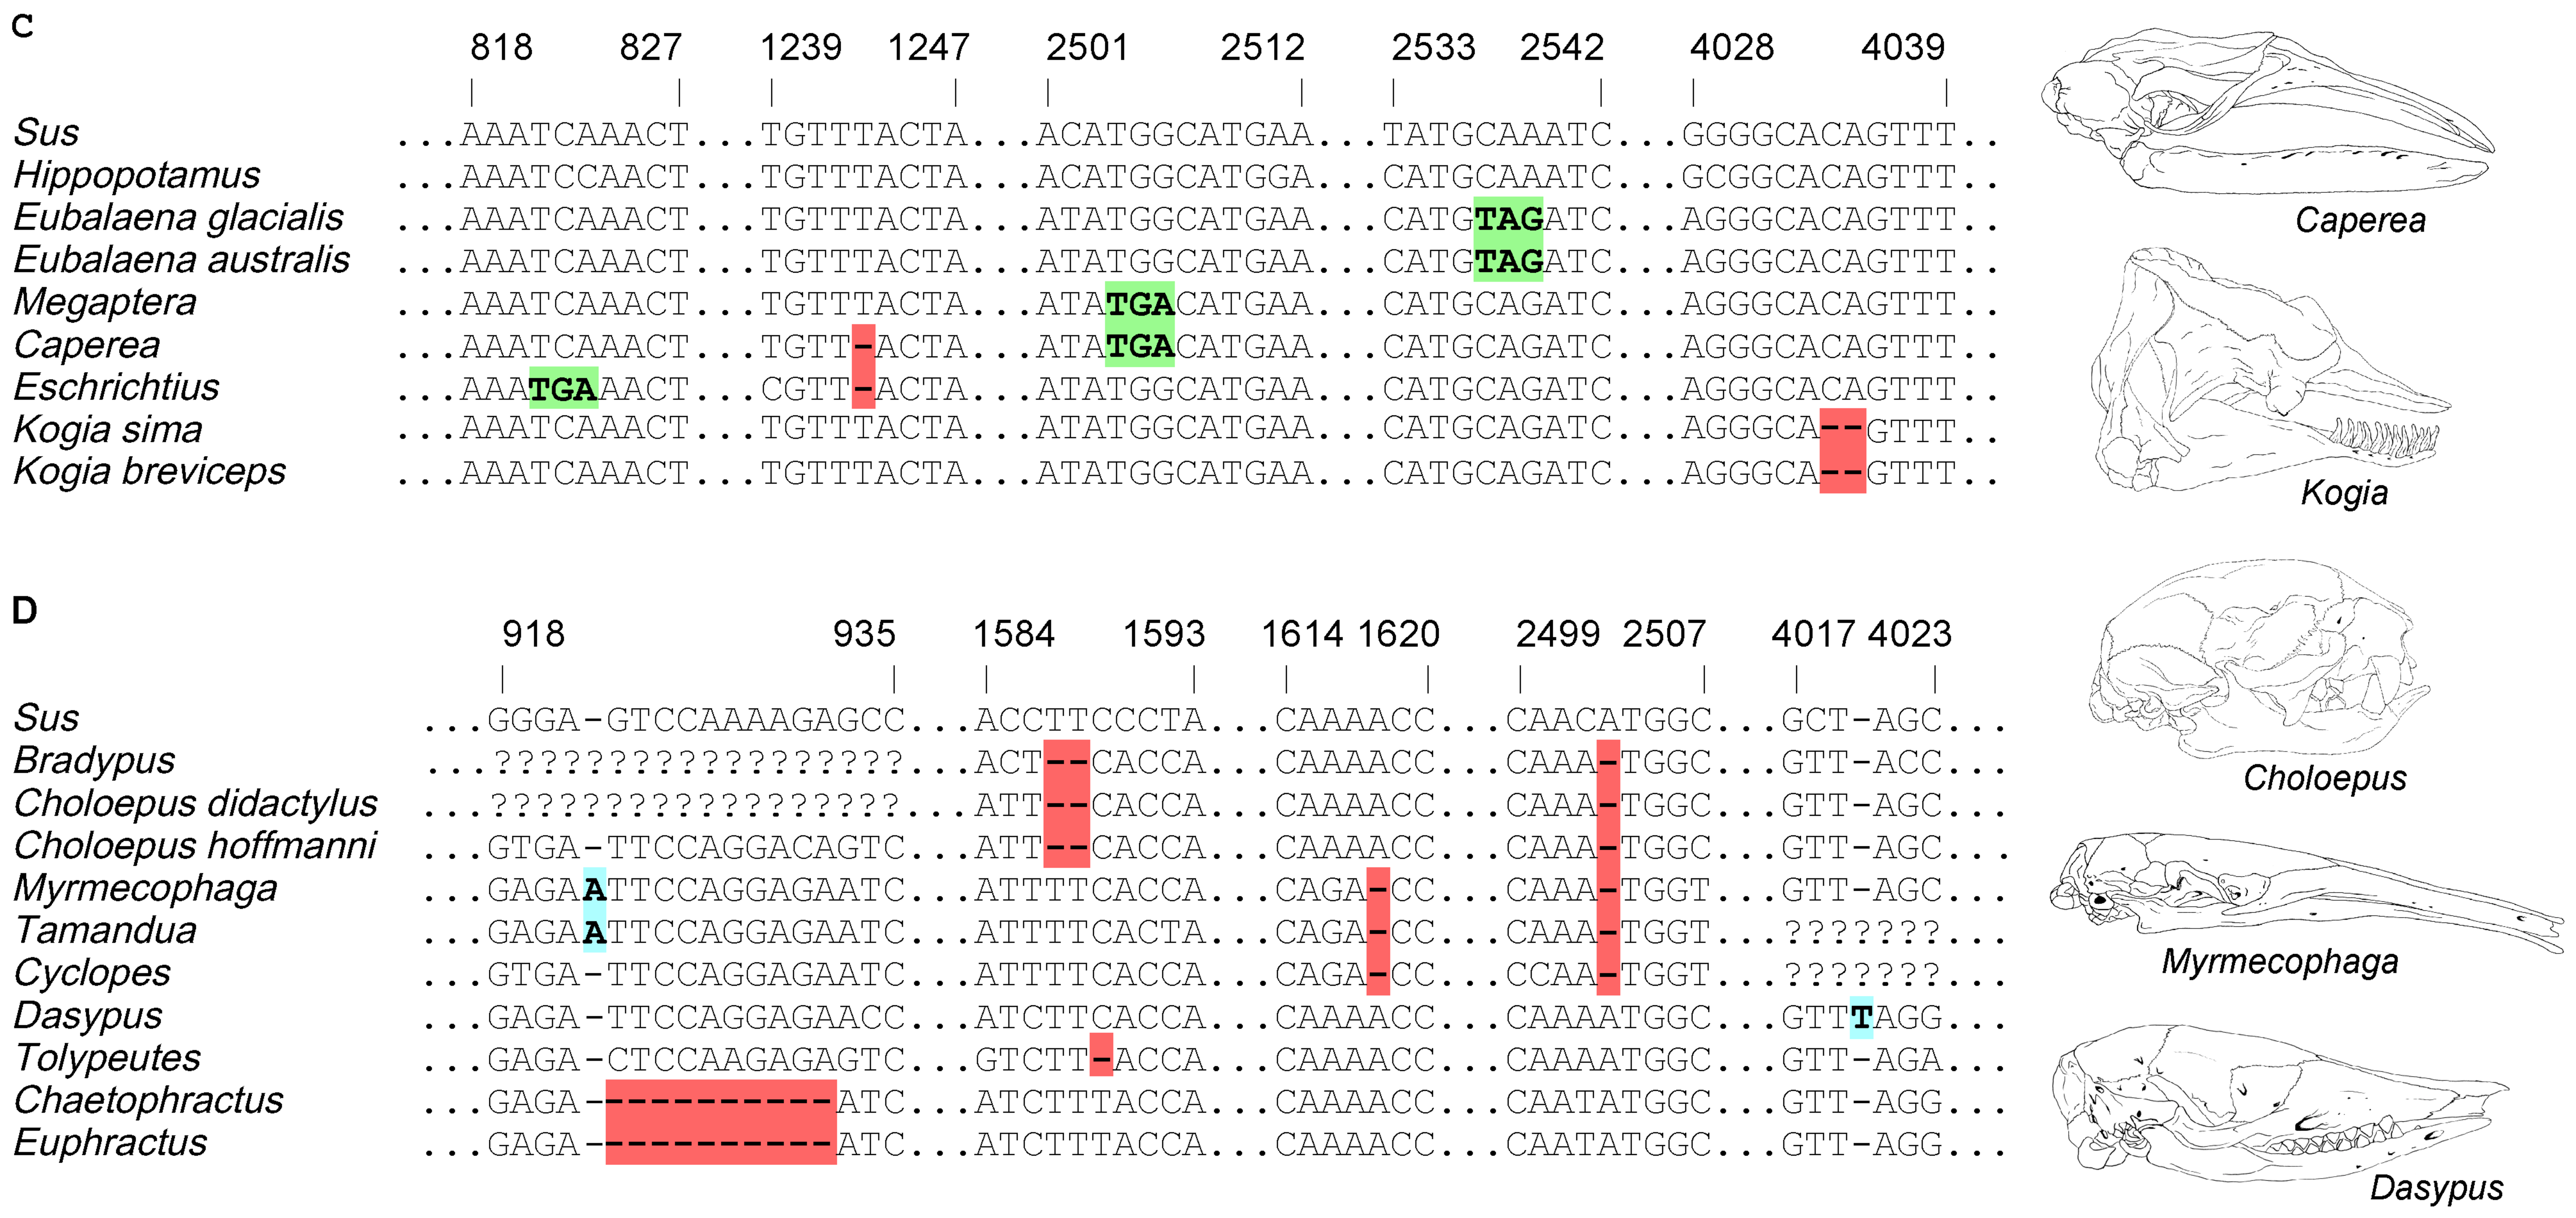
\includegraphics[width=\textwidth]{Journal_figs/genetic_drift/Enamelin/Enamlin.pdf}
\end{center}
\caption{Examples of frameshift mutations (insertions blue, deleteions
  red) and premature stop codons in Enamlin in Cetacea and
  Xenarthra. Figure taken from \citeauthor{Meredith:09}} \label{fig:Enamlin_coding}  
\end{figure} 

\marginnote{
``Rudimentary organs may be compared with the letters in a word, still
retained in the spelling, but become useless in the pronunciation, but
which serve as a clue .. for its derivation.'' 
}  %http://darwin-online.org.uk/Variorum/1859/1859-456-dns.html
\graham{get Darwin page number etc}

The protein Enamlin is a key structural protein involved in the outer cap of enamel on teeth. Various mammals have secondarily evolved to lack enamel on their teeth, or to lack teeth entirely, as because changing diet allowed selection to become was relaxed on having hard teeth. For example,  two-toed sloths ({\it Choloepus}); Pygmy sperm whales ({\it Kogia}); aardvark {\it Orycteropus}) lack  enamel on teeth. While others have lost their teeth entirely e.g. giant anteaters ({\it Myrmecophaga}) and Baleen whales. Due to this relaxation of constraint of the phenotype, loss of selective function pseudogenizing substitutions, premature stop codons and frameshift mutations, have
accumulated in the gene Enamlin (see Figure \ref{fig:Enamlin_coding}
for examples).  \citeauthor{Meredith:09} sequenced Enamlin across a
range of species and found that none of the species with Enamel have frameshift
mutations in Enamlin, while 17/20 of species that lack Enamel or teeth have
frameshifts in Enamlin and all of them carry premature stop codons
(Figure \ref{fig:Enamlin_phylo}). 

\begin{figure}
\begin{center}
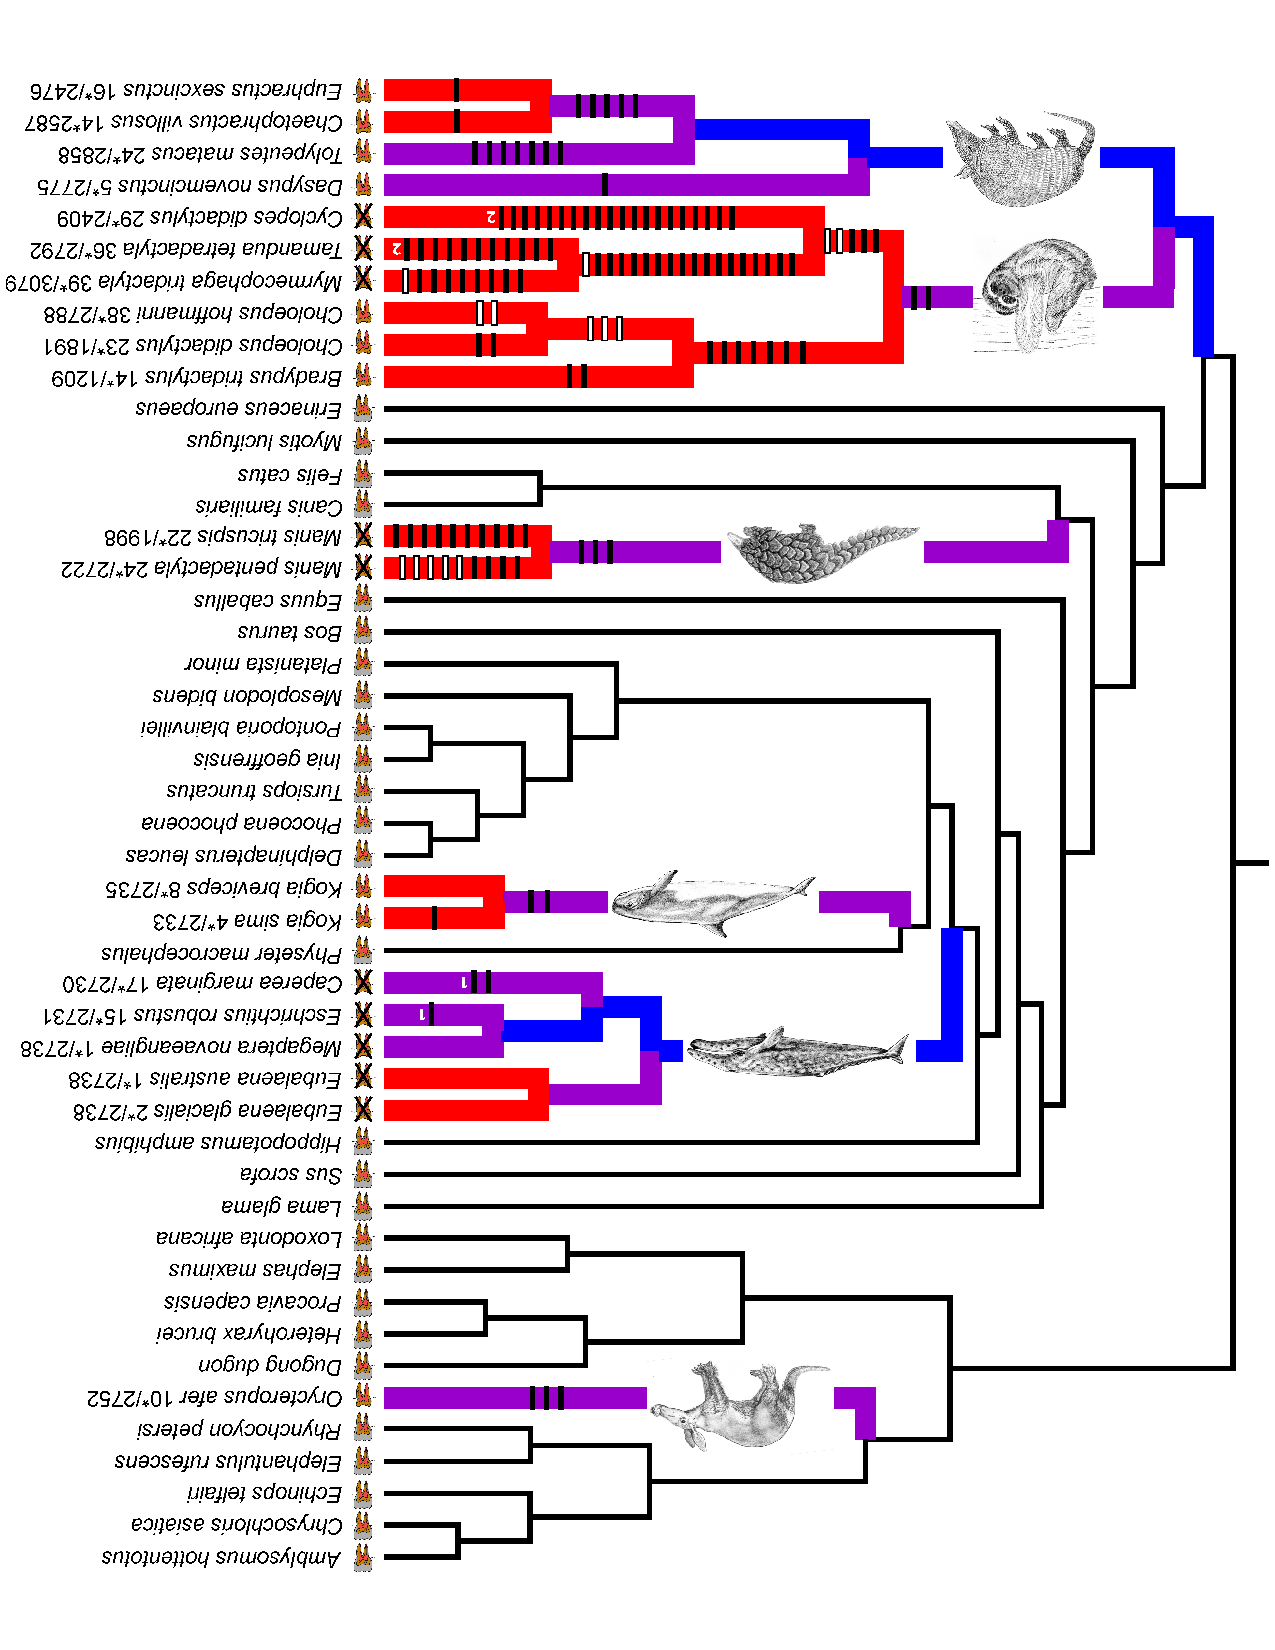
\includegraphics[width=0.8 \textwidth]{Journal_figs/genetic_drift/Enamelin/Enamlin_phylo.pdf}
\end{center}
\caption{The tooth symbol next to each taxon shows whether they have
  teeth, lack enamel, or lack teeth. Branches of the phylogeny are coloured by whether their
  Enamlin is functional (black), pre-mutation (blue), mixed (purple),
  and pseudogenic (red). The black and white vertical bars on branches show frameshift
  mutations.  The Numbers after taxon names indicate minimum number of
  stop codons in the sequence /  the length of the sequence.} \label{fig:Enamlin_phylo}  
\end{figure} 

The branches of the Enamlin phylogeny with a functional Enamlin gene (black) had an estimated $\dNdS= 0.51$ consistent with the protein evolving in a constrained manner. While the branches with a pseudogenized Enamlin
had $\dNdS = 1.02$ consistent with the gene evolving an unconstrained
way. The branches where the gene was likely transitioning from a functional
to non-function state (premutation and mixed, blue and purple) had an intermediate values of
$\dNdS=0.83-0.98$ consistent with them transitioning from a constrained to unconstrained mode of protein evolution somewhere along these branches of the phylogeny.

%\begin{question}
%Enamlin was pseudogenized somewhere along the branch leading to
%Aardvarks ({\it Orycteropus}). This branch has $\dNdS=0.75$
% https://journals.plos.org/plosgenetics/article?id=10.1371/journal.pgen.1000634#pgen.1000634.s007
%dawn pangloin
%https://commons.wikimedia.org/wiki/File:Eomanis_waldi_4.jpg
%% aadvark https://www.flickr.com/photos/internetarchivebookimages/20514695666/in/photolist-xfPbiq-xUcng7-xCyGQA-xdRRQ3-wPMGZr-tFgYfN-wPMPkT-tDahHQ-xuc4KM-xKR4u3-xUkupQ-w88zeU-xMia2r-sp4Aq5-x1wNyZ-xMi46D-tDaCr7-sJE2X4-tFB8Lc-wHWiNj-tp8AUk-tFvh4R-xu3M7w-toUVwN-wYWgVi-w34vHn-x9xAfL-wWhnso-ovvmHE-tG5AgB-xdUzWD-y82dEG-xCA7kx-xV5xWg-wYc33H-wYbFdX-wYbBMP-xUcjpL-xKQjHw-xJmBQU-xKPwEQ-xLEzv4-xu3wHJ-xLEg9V-xnA6Lr-x684wQ-wZNgpq-wYcVbh-wZtb3F-wYbJLh
%%% w1 t/T + w2(T-t)/T = wT
%% https://journals.plos.org/plosgenetics/article?id=10.1371/journal.pgen.1000634#pgen.1000634.s007



%\end{question}
\paragraph{Adaptive evolution and $\dNdS$.}
Clearly genes are not only subject to neutral and deleterious mutations, beneficial mutations must also arise and fix from from time to time. 
Lets assume that a fraction $B$ of non-synonymous mutations that arise are
beneficial such that $2 N \mu B$ beneficial mutations arise per generation. Each of this mutations reach fixation in the population with probability $f_B$. This fixation
probability may be much higher than that of neutral mutations (we'll
discuss how to calculate the fixation probability for beneficial
alleles in Chapter \ref{Selection_Stochasticity}).  If $2T$ generations of divergence have
elapsed between the two populations 
\begin{equation}
dN=2T (1-C - B) \mu  + 2T \times (2 N \mu B) \times  f_B
\end{equation}
Then
\begin{equation} 
\dNdS = (1-C-B) +  2 N B f_B
\end{equation}
Note that this means that our estimates of $C$ using $1-\dNdS$ will be
a  lower bound on the true constraint if even a small fraction of
mutations are beneficial.
However, genes may still evolve in a constrained way
(i.e. $\dNdS<1$)  if adaptive substitutions are common at a gene if
they are outweighed by the loss of potential substitutions to negative selection.

\paragraph{loss of constraint} While most genes evolve under constraint, we can find examples of
genes that are evolving in a less constrained manner. The simplest
example of this is where the gene has lost function, e.g. has recently
become pseudogenized. Along branches of the phylogeny where all the
constraint against non-synonymous mutation has
been lost then $\dNdS=1$. We can also identify cases where the gene
is evolving more rapidly at the protein level than at synonymous
sites, i.e. $d_N/d_S > 1$, corresponding to cases of rapid change due
to positive selection. 

\begin{figure}
\begin{center}
\includegraphics[width=0.8 \textwidth]{Journal_figs/genetic_drift/Yang_lysozyme/Yang_lysozyme.pdf}
\end{center}
\caption{A phylogram for the primate lysozyme gene redrawn from
  \citeauthor{Yang:98}. For each branch the numbers give the estimated average
number of non-synonymous to synonymous changes in the lysozyme protein.} \label{fig:lysozyme}  
\end{figure} 

\begin{marginfigure}
\begin{center}
\includegraphics[width=0.8 \textwidth]{illustration_images/Genetic_drift/Colobus/19792029373_fcce706e67_k.jpg}
\end{center}
\caption{Abyssinian black-and-white colobus ({\it Colobus guereza}). Brehm's Tierleben,  Brehm,
  A.E. 1893. A member of the leaf-eating Colobines.} \label{fig:Colobus}  
\end{marginfigure} 

\begin{marginfigure}
\begin{center}
\includegraphics[width=0.8  \textwidth]{illustration_images/Genetic_drift/Hoatzin/14747388314_85798ba97e_z.jpg}
\end{center}
\caption{ (hoatzin ({\it Opisthocomus hoazin}). A history of birds
  Pycraft, W.P. 1910.  A leaf-eating bird.} \label{fig:hoatzin}  
\end{marginfigure} 
A classic example of looking for adaptive evolution using dN/dS is the
evolution of the lysozyme protein in primates \citep{Messier:97,Yang:98}, see
the phylogeny in Figure \ref{fig:lysozyme}. The lysozyme protein is
a key component for the breakdown of bacterial walls. It shows very
fast protein evolution notably on the lineages leading to apes (e.g. gibbons
and humans) and Colobines (e.g. colobus and langur monkeys). Colobines have leaf-based diets. They digest
these leaves by fermentation with bacteria in their foregut, and use lysozymes to break down the bacteria to extract energy from the
leaves. In Colobines the lysozyme protein has evolved to work well in the high-PH environment of the stomach. Remarkably the Colobine
lysozyme has convergently evolved this activity via very similar amino-acid changes at 5 key residuals as in cows and Hoatzins (a leaf
eating bird). 

\paragraph{The Mcdonald-Kreitman test}
\citet{mcdonald:91} devised a simple test of the neutral theory of molecular
evolution at a gene (building on the conceptually similar HKA
test\cite{HKA}. They partitioned polymorphism and fixed differences into 
nonsynonymous and synonymous changes:
\begin{center}
%\begin{table}
\begin{tabular}{ccc}
 & Poly. & Fixed \\
\hline 
Non-Syn. &    $P_N$  &   $D_N$  \\
Syn. &    $P_S$   &     $D_S$   \\
Ratio & $P_N/P_S$ & $D_N/D_S$
\end{tabular}
\end{center}

Under neutral theory we expect a smaller number of non-synonymous to
synonymous fixed differences ($P_N/P_S < 1$) but exactly the same
expectation holds for polymorphism
($P_N/P_S$). To see this denote the total time on the coalescent genealogy within the species as
$T_{tot}$ and the total time for fixed differences by $T_{div}'$ then:

\begin{marginfigure}
\begin{center}
\includegraphics[width=0.8 \textwidth]{figures/Coalescent/MK_tree.pdf}
\end{center}
\caption{ } \label{fig:MK_tree}
\end{marginfigure}

\begin{center}
\begin{tabular}{ccc}
 & Poly. & Fixed  \\
 \hline
Non-Syn. &    $\mu_N T_{tot}$  &   $\mu_N  T_{div}'$ \\
Syn. &    $\mu_S T_{tot}$   &     $\mu_S  T_{div}'$  \\
Ratio & $\mu_N/\mu_S$  & $\mu_N/\mu_S$
\end{tabular}
\end{center}
Therefore, we expect the ratio of non-synonymous to synonymous changes
to be the same for polymorphism and divergence. We can test this expectation of equal ratios via the standard G-test of a $2
\times 2$ table.

\subsection{Neutral diversity and population structure}
%%this section was moved from the coalescent chapter
Up to now we have assumed that our alleles that we have modelled in the
coalescent setting are drawn from a randomly mating population such
that any pair of lineages is equally likely to coalesce with each
other. However, when there is population structure this assumption is
violated. \\

We have previously written the measure of population structure
$\fst$ as
\begin{equation}
\fst = \frac{H_T-H_S}{H_T}
\end{equation}
where $H_S$ is the probability that two alleles sampled at random from a
subpopulation differ, and $H_T$ is the probability that two alleles
sampled at random from the total population differ. 

\paragraph{A simple population split model}
Imagine a population of constant size of $N_e$ diploid individuals that
$\tau$ generations in the past split into two daughter populations (sub-populations)
each of size $N_e$ individuals, who do not subsequently exchange
migrants. In the current day we sample an equal number of alleles
from both subpopulations.

Consider a pair of alleles sampled within one of our
sub-populations, they have experienced a population of size $N_e$
and so the probability that they differ is $H_S = \theta/(1+\theta)$
(where $\theta=4N_e\mu$).
The heterozygosity in our total population is a little more tricky to
calculate. Assuming that we equally sample both sub-populations, when we draw two alleles from our total
sample, $50\%$ of the time they are drawn from the same
subpopulation and $50\%$ of the time they are drawn from different
subpopulations. Therefore, our total heterozygosity is given by
\begin{equation}
H_T = \half H_S + \half H_B
\end{equation}
where $H_B$ is the probability that a pair of alleles drawn from our
two different sub-populations differ from each other. Our pair of
alleles can not find a common ancestor with each other for at least $\tau$
generations into he past as they are in distinct populations (not
connected by migration). The probability that one or other of them
mutates in this time is $1-(1-\mu)^{2T}$. With probability
$(1-\mu)^{2T} $ neither of our alleles mutate in the $T$ generations
back in time before they find themselves back in the combined ancestral 
population. Conditional on failing to mutate before the combined ancestral
population, the probability that they do manage to mutate before
coalescing in that population of size $N_e$ is
$\theta/(\theta+1)$. Putting these components together
\begin{equation}
H_B = \left( 1-(1-\mu)^{2T} \right) + (1-\mu)^{2T}
  \frac{\theta}{\theta+1} 
\end{equation}
We can plug this into our expression for $H_T$, and then that in turn
into $\fst$.

\begin{figure}
\begin{center}
\includegraphics[width= 0.8 \textwidth]{figures/drift_split.png}
\end{center}
\caption{Change in allele frequencies following a population split.} \label{fig:drift_split}  
\end{figure} 

To understand this better we can make a simple
approximation based on our mutation rate being very low, such that
$N_e \mu \ll 1$ so $H_S \approx
4N_e\mu$, and that $\mu \ll 1$ and $\mu T \ll 1$. Assuming this, then  
\begin{equation}
H_B \approx 2 \mu T + 4N_e\mu. 
\end{equation}
So that 
\begin{equation}
\fst \approx \frac{ \mu T}{\mu T +  4N_e\mu }  %= \frac{ T}{ T +  4N_e }
\end{equation}
note that $\mu$ cancels out of this. In this simple toy model $\fst$
is increasing because the amount of between population diversity 
increases with the divergence time of the two populations (initially
linearly with $T$). It does so at a rate
give by $\nicefrac{T}{(4N_e)}$ so that differentiation will be higher
between populations separated by long divergence times or with small
effective population sizes.

\begin{question}
The gorilla lineage split from the human-chimp lineage $\sim$7 million years ago. Let’s assume that this speciation event occurred instantaneously in allopatry with no subsequent gene flow. \\
{\bf A)}	What is the probability of that gorilla is not an outgroup to human and chimp at a single locus?\\
{\bf B)}	It has been estimated that the gorilla lineage is not an outgroup at around ~30\% of autosomal loci. What effective population size would you need to assume to explain this observation? Is that only plausible explanation?\\
{\bf C)}	The gorilla lineage is an outgroup for large portions of the X chromosome, what is a plausible explanation for this finding?
\end{question}

\paragraph{A simple model of migration between an island and the mainland.}
We can also use the coalescent to think about patterns of
differentiation under a simple model of migration drift
equilibrium. Lets consider a small island population that is relatively isolated
from a large mainland population, and that both of these populations
are constant in size. We'll assume that the expected heterozygosity
for a pair of alleles sampled on the mainland is $H_M$.

Our island has a population size
$N_{I}$ that is very small compared to our mainland population.
Each generation some low fraction $m$ of our individuals on the
island have migrant parents from the mainland the generation
before. Our island may also send migrants back to the mainland, but
these are a drop in the ocean compared to the large population size on
the mainland and their effect can be ignored. 


If we sample an allele on the island back and trace its ancestral
lineage backward in time, each generation our ancestral allele have a low
probability $m$ of being descended from the mainland in the proceeding
generation (if we go far enough the allele eventually has to be
descended from an allele on the mainland). The probability that a pair of alleles sampled on the
island are descended from a shared recent common ancestral allele on the island, is the
probability that our pair of alleles coalesce before either lineage
migrates. For example, the probability that our pair of alleles
coalesce $t+1$ generations back is 
\begin{equation}
\frac{1}{2N_I}(1-m)^{2(t+1)} \left(1-\frac{1}{2N_I} \right)^{t} \approx
\frac{1}{2N_I} \exp\left( -t\left (\frac{1}{2N_I} + 2m\right) \right),
\end{equation}
with the approximation following from assuming that $m \ll 1$ \& $\frac{1}{(2N_I)}
\ll 1$ (note that this is very similar to our derivation of
heterozygosity above). The probability that our alleles coalescence before either one
of them migrates off the island, irrespective of the time, is
\begin{equation}
\int_0^{\infty} \frac{1}{2N_I} \exp\left( -t\left (\frac{1}{2N_I} +
2m\right) \right) dt = \frac{\nicefrac{1}{(2N_I)}}{\nicefrac{1}{(2N_I)} +
    2m}.
\end{equation}

Lets assume that the mutation rate is very low such as it is very
unlikely that the pair of alleles mutate before they coalesce on the
island. Therefore, the only way that the alleles can be different from
each other is if one or other of them migrates to the mainland, which
happens with probability  
\begin{equation}
  1 - \frac{\nicefrac{1}{(2N_I)}}{\nicefrac{1}{(2N_I)} + 2m}
\end{equation}
Conditional on one or other of our alleles migrating to the mainland,
both of our alleles represent independent draws from the mainland and
so differ from each other with probability $H_M$. Therefore, the level of
heterozygosity on the island is given by
\begin{equation}
  H_I = (1 - \frac{\nicefrac{1}{(2N_I)}}{1/(2N_I) + 2m})H_M
\end{equation}
So the reduction of heterozygosity on the island compared to the
mainland is
\begin{equation}
  F_{IM} = 1- \frac{H_I}{H_M} = \frac{\nicefrac{ 1}{(2N_I)}}{\nicefrac{1}{(2N_I)} + 2m} = \frac{ 1 }{1 + 4N_Im}.
\end{equation}
The level of inbreeding on the island compared to the mainland will
be high in the migration rate is low and the effective population size
of the island is low, as allele frequencies on the island are drifting
and diversity is not being replenished on the island by migration. The
key parameter here is the number individuals on the island replaced by
immigrants from the mainland each generation ($N_I m$).

We have framed this as being about the reduction in genetic diversity on the
island compared to the mainland. However, if we consider collecting 
individuals on the island and mainland in proportion to population
sizes the total level of heterozygosity would be $H_T=H_M$, as samples
from our mainland would greatly outnumber those from our
island. Therefore, considering our island our sub-population we have
derived another simple model of $F_{ST}$.

\begin{question}
You are investigating a small river population of sticklebacks, which receives infrequent migrants from a very large marine population. At a set of (putatively neutral biallelic markers the freshwater population has frequencies:\\
0.2, 0.7, 0.8\\
at the same markers the marine population has frequencies:\\
0.4, 0.5 and 0.7.\\
 From studying patterns of heterozygosity at a large collection of markers, you have estimated the long term effective size of your freshwater population is 2000 individuals.\\
What is your estimate of the migration rate from the marine
populations into the river?
\end{question}

\paragraph{Incomplete lineage sorting}

Because it can take a long time for an polymorphism to drift up or down in
frequncy, multiple population splits may occur during the transit of
an allele. This can lead to incongruence between the overall
population tree  and the information about relationships present at
individual loci. In Figure \ref{fig:NoILS_poly} and \ref{fig:ILS_poly}
we show a simulations
of three populations where the bottom population splits off from the
other two first, followed by the subsequent spliting of the the top
and the middle population. We start both simulations with a newly
introduced red allele being polymorphic in the combined ancestral
polymorphism. The most likely fate of this allele is that it is
quickly lost from the population, but sometimes the allele can drift
up in frequency and be polymorphic when the populations split, as the
alleles in our two figures have done. If the allele is lost/fixed in
the descendent populations before the next population split our allele
configuration will agree with the population tree, as it does in
Figure  \ref{fig:NoILS_poly}. However, if the allele persists as a
polymorphism in the ancestral population till the top and the middle
populations split, then the allele can fix in one of these populations
and not the other. Such an event can lead to a substitution pattern
that disagrees with the population tree, as in \ref{fig:ILS_poly}.  If
we were construct a phylogeny using the variation we would see a
disagreement between the gene tree and species tree.

\begin{figure}
\begin{center}
\includegraphics[width=\textwidth]{figures/Genetic_drift/ILS/no_ILS.pdf}
\end{center}
\caption{  } \label{fig:NoILS_poly} 
\end{figure}

\begin{figure}
\begin{center}
\includegraphics[width=\textwidth]{figures/Genetic_drift/ILS/ILS.pdf}
\end{center}
\caption{  } \label{fig:ILS_poly} 
\end{figure}

A natural, pedigree analogy to this is the fact that while two
biological siblings are morely closely related to each other than
either is to their cousin, at any given locus one of the siblings can
shared an allele IBD with their cousin that they do not share with
their own sibling, due to the randomness of mendelian segregating down their
pedigree. The average relatedness of the individuals/population disagrees
with the patterns of relatedness at a particular locus.

\begin{marginfigure}
\begin{center}
\includegraphics[width=\textwidth]{illustration_images/Genetic_drift/Poephila_cincta_finch/Poephila_cincta_finch.png}
\end{center}
\caption{Banded Grass Finch ({\it P. cincta}). Illustration by
  Elizabeth Gould. Birds of Australia Gould J. 1840. } \label{fig:Poephila_cincta} 
\end{marginfigure}

\citeauthor{jennings:05} sequenced a single allele from three
different species of Australian grass finches (Poephila); two sister species
of long-tailed finches ({\it Poephila acuticauda} and {\it P. hecki})
and the black-throated finch ({\it Poephila cincta}, see Figure \ref{fig:Poephila_cincta}). They collected
sequence data for 30 genes, and constructed phylogenetic gene trees
at each of these loci, resulting in 28 well resolved gene trees. 
16 gene trees of the gene trees showed {\it
  P. acuticauda} and {\it P. hecki} as sisters with {\it P. cincta})
(the tree ((A,H),C)~). While for twelve genes the gene tree was
discordant with the population tree: for seven of their genes  {\it P. hecki}
fell as an outgroup to the other two; and at five {\it P. acuticauda} fell as an outgroup (the trees ((A,C),H) and
((H,C),A) respectively). 

\begin{figure}
\begin{center}
\includegraphics[width=\textwidth]{figures/Genetic_drift/ILS/ILS_coal_cartoon.pdf}
\end{center}
\caption{The population tree of three populations ((A, B), C) is shown
blocked out with black shapes. Two different coalescent trees are
relating a single allele drawn from A, B, and C are shown with thinner lines.} \label{fig:ILS_cartoon} 
\end{figure}
Lets use the coalescent to understand this discordance between gene
trees and species trees. Lets assume that two sister populations
(A \& B) split $t_1$ generations in the past, with a
deeper split from a third outgroup population (C) $t_2$ generations in the
past. We'll assume that there's no gene flow among our populations
after each split. We can trace back the ancestral lineages of our three alleles. The
first opportunity for the A \& B lineages to coalesce is $t_1$
generations. If they coalesce with each other in their shared
ancestral population before $t_2$ in the past, left side of
\ref{fig:ILS_cartoon}, their gene tree will
definitely agree with the population tree. So the only way for the gene
tree to disagree with the population tree is for the A \& B lineages
to fail to coalesce in their shared ancestral population, this happens
with probability $\left(1 - \nicefrac{1}{2N}\right)^{t_2-t_1}$. We'll
get a discordant gene tree, if A
\& B make it back to the shared ancestral population with C without
coalescing, and then one or other of them coalesces with the C
lineage first. This happens with probability $2/3$, as at the first
pairwise-coalescent event there are are three possible pairs two of
which (A \& C  and B \$ C ) result in a discordant tree. So the
probability that we get a coalescent tree that is discordant with the
population tree is
\begin{equation}
\frac{2}{3} \left(1 - \nicefrac{1}{2N}\right)^{t_2-t_1}.
\end{equation}
Thus we should expect gene-tree population-tree discordance when
population split in rapid succession, and/or population sizes are
large. 
\begin{question}
Lets return to \citeauthor{jennings:05}'s Australian grass finches
example, they estimated that the ancestral population size of our two
long-tailed finches was four hundred thousand. What is your best
estimate of the inter-speciation time, i.e. $t_2-t_1$? 
\end{question}

\paragraph{Testing for gene flow.} 

We often want to test whether gene flow has occurred between populations. For example, we might want to establish a case
that interbreeding between humans and Neanderthals occurred or demonstrate that
gene flow occurred after two populations began to speciate. 
A broad range of methods have been designed to test for gene flow, and
toestimate gene flow rates, based on neutral expectations. Here'll we
briefly just discuss one method based on
some simple coalescent ideas.  Above we assumed that gene-tree population-tree discordance was due to
incomplete lineage sorting due to populations rapidly
spliting. However, gene flow among populations can also lead to gene-tree discordance.
While both ILS and gene flow can lead to discordance, under
simplifying assumptions ILS implies more symmetry in how these
discordancies manifest themselves.\\


\begin{figure}
\begin{center}
\includegraphics[width=\textwidth]{figures/Genetic_drift/ILS/ABBA_BABA_coal.pdf}
\end{center}
\caption{ In boh the left and and right trees ILS has occurred between our single lineages sampled from populations A, B, and C. Imagine that population D, is an somewhat distant outgroup
such that the lineages from A-C (nearly) always coalesce with each
other, before coalescing with D. The small dash on the branch
indicates the mutation A$\rightarrow$B occuring, giving rise to the
mutational patter shown at the bottom. } \label{fig:ABBA_BABA} 
\end{figure}

Take a look at Figure \ref{fig:ABBA_BABA}. \graham{switch to
  1-4?}. In both cases the lineages from A and B fail to coalesce in
their initial shared ancestral population, and one or other of them
coalesces with the lineage from C first. Each option is equally
likely, therefore the mutational patterns ABBA and BABA are equally
likely to occur under ILS.  \sidenote{here we have to assume no
  structure in the ancestral population.}

However, if gene flow occurs from population C into population B the
lineage from B can more recently coalesce with lineage C, and so we
should see more ABBAs than BABAs. To test for this we can sample four
sequences from our populations and count up the number of sites that
show the two mutational patterns consistent with the gene-tree discordance $n_{ABBA}$ and
$n_{BABA}$ and take 
\begin{equation}
\frac{n_{ABBA}-n_{BABA}}{n_{ABBA}+n_{BABA}}
\end{equation}
this statistic will have expectation zero if the gene-tree discordance
is due to ILS, and be skewed negative if gene flow
occurred from C into B (positive if gene flow occurred from C into A).


%\section{Correlations between loci, linkage disequilibrium, and recombination}

%</source-file>

Up to now we have been interested in correlations between alleles at the
same locus, e.g. correlations within individuals (inbreeding) or between
individuals (relatedness). We have seen how relatedness between parents affects the extent to which their offspring is inbred. We now turn to 
correlations between alleles at different loci. To understand
correlations between loci we need to understand recombination.\\


\paragraph{Recombination}  Lets
consider an individual heterozygous for a $AB$ and $ab$
haplotype. If no recombination occurs between our two loci in this
individual, then these two haplotypes will be transmitted intact to
the next generation. While if a recombination (or more generally an
odd number of recombinations) occurs between our two loci on the
haplotype transmitted to the child then $\tfrac{1}{2}$ the time the
child receives a $Ab$ haplotype and $\tfrac{1}{2}$ the time the child
receives a $aB$ haplotype. So recombination is breaking up the
association between loci. We'll define the recombination fraction ($r$) to be
the probability of an odd number of recombinations between our loci.
In practice we'll often be interested in relatively short regions
where recombination is relatively rare, and so we might think that
$r=r_{BP}L \ll 1$, where $r_{BP}$ is the average recombination rate
per base pair (typically $\sim 10^{-8}$) and L is the number of base
pairs separating our two loci.\\



\paragraph{Linkage disequilibrium}
The (horrible) phrase linkage
disequilibrium (LD) refers to the statistical non-independence
(i.e. a correlation)  of
alleles at different loci. Our two loci, which segregate alleles $A/a$ and $B/b$, have allele
frequencies of $p_A$ and $p_B$ respectively. The frequency of the two locus haplotype is $p_{AB}$,
and likewise for our other three combinations. If our loci were
statistically independent then $p_{AB} = p_Ap_B$, otherwise $p_{AB} \neq p_Ap_B$
We can define a covariance between the $A$ and $B$ alleles at our two loci as
\begin{equation}
D_{AB} = p_{AB} - p_Ap_B
\end{equation}
and likewise for our other combinations at our two loci
($D_{Ab},~D_{aB},~D_{ab}$). These $D$ statistics are all closely
related to each other as $D_{AB} = - D_{Ab}$ and so on. Thus we only
need to specify one $D_{AB}$ to know them all, so we'll drop the
subscript and just refer to $D$. Also a handy result is that we can rewrite our haplotype
frequency $p_{AB}$ as
\begin{equation}
p_{AB} = p_Ap_B+D. \label{eqn:ABviaD}
\end{equation}
If $D=0$ we'll say the two loci are in linkage equilibrium, while if
$D>0$ or $D<0$ we'll say that the loci are in linkage
disequilibrium (we'll perhaps want to test whether $D$ is
statistically different from $0$ before making this choice). You should be careful to keep the concepts of linkage
and linkage disequilibrium separate in your mind. Genetic linkage refers to the
linkage of multiple loci due to the fact that they
are transmitted through meiosis together (most often because the
loci are on the same chromosome). Linkage disequilibrium merely refers
to the correlation between the alleles at different loci, this may in
part be due to the genetic linkage of these loci but does not
necessarily imply this (e.g. genetically unlinked loci can be in LD
due to population structure). \\

Another common statistic for summarizing LD is $r^2$ which we write as
\begin{equation}
r^2 = \frac{D^2}{p_A(1-p_A) p_B(1-p_B) }
\end{equation}
as $D$ is a covariance, and $p_A(1-p_A) $ is the variance of an allele
drawn at random from locus $A$, $r^2$ is the squared correlation
coefficient.    \\


{\bf Question.} You genotype 2 bi-allelic loci (A \& B) segregating in two mouse subspecies (1 \& 2) which mate randomly among themselves, but have not historically interbreed since they speciated. On the basis of previous work you estimate that the two loci are separated by a recombination fraction of 0.1. The frequencies of haplotypes in each population are:
\begin{center}
\begin{tabular}{|c|cccc|}
\hline
Pop    & $p_{AB}$    & $p_{Ab}$ &    $p_{aB}$ &    $p_{ab}$\\
\hline
1 &    .02    & .18 &     .08 &    .72\\
2&    .72 &    .18 &    .08 &    .02\\
\hline
\end{tabular}
\end{center}

{\bf A)} How much LD is there within populations, i.e. estimate D?\\

{\bf B)} If we mixed the two populations together in equal proportions what value would D take before any mating has had the chance to occur? \\



\paragraph{The decay of LD due to recombination}
We will now examine what happens to LD over the generations if we
only allow recombination to occur in a very large population (i.e. no
genetic drift, i.e. the frequencies of our loci follow their expectations). To do so consider the frequency of our $AB$ haplotype in the next generation
$p_{AB}^{\prime}$. We lose a fraction $r$ of our $AB$ haplotypes to
recombination ripping our alleles apart but gain a fraction $rp_A p_B$ per generation from other
haplotypes recombining together to form $AB$ haplotypes. Thus in the
next generation
\begin{equation}
p_{AB}^{\prime} = (1-r)p_{AB} + rp_Ap_B
\end{equation}
this last term here is $r(p_{AB}+p_{Ab})(p_{AB}+p_{aB})$, which
multiplying this out is the
probability of recombination in the different diploid genotypes that
could generate a $p_{AB}$ haplotype. \\

We can then write the change in the frequency of the $p_{AB}$
haplotype as
\begin{equation}
\Delta p_{AB} = p_{AB}^{\prime} -p_{AB} = -r p_{AB} + rp_Ap_B = - r D
\end{equation}
so recombination will cause a decrease in the frequency of $p_{AB}$ if
there is an excess of $AB$ haplotypes within the population ($D>0$), and an
increase if there is a deficit of $AB$ haplotypes within the
population ($D<0$). Our LD in the next generation is $D^{\prime} =
p_{AB}^{\prime}$, so we can rewrite the above eqn. in terms of the
$D^{\prime} $
\begin{equation}
D^{\prime}= (1-r) D
\end{equation}
so if the level of LD in generation $0$ is $D_0$ the level $t$
generations later ($D_t$) is
\begin{equation}
D_t=  (1-r)^t D_0
\end{equation}
so recombination is acting to decrease LD, and it does so
geometrically at a rate given by $(1-r)$. If $r \ll 1$ then we can
approximate this by an exponential and say that   
\begin{equation}
D_t \approx  D_0 e^{-rt}
\end{equation}\\



{\bf Q C)} You find a hybrid population between the two mouse subspecies
described in the question above, which appears to be comprised of equal proportions of ancestry from the two subspecies.  You estimate LD between the two markers to be 0.0723. Assuming that this hybrid population is large and was formed by a single mixture event, can you estimate how long ago this population formed? \\

%\subsection{Testing for departures from HWE.}
%Note the form of $\hat{F}$ \eqref{eqn:FhatHO} is the same as the $X^2$
%statistic, and so we can test for a deviation from hardy-weinberg  $X^2$


%\subsection{Population structure}
%The question naturally arises at this point: what reference population
%(i.e. what allele frequency) do we use to calculate $\hat{F}$? If we are %calculating the inbreeding coefficient
%of an English person do we use the frequencies of the town of that
%person, of England, of the United Kingdom, or of the World?



%\gc{Include the HapMap exercise here?}


%==One locus models of selection==
%<source-file filename="one_loc_sel_models.tex" display="one_loc_sel_models.wrapped.latexml.xhtml">

\newpage


\chapter{Phenotypic Variation and the Resemblance Between Relatives.}

\newthought{The distinction between genotype and phenotype} is one of the most useful ideas in biology.\cite{Johannsen:1911} 
The genotype of an individual (the genome), for most purposes, is decided when
the gametes fuse to form a zygote (individual). The phenotype of an individual represents any
measurable aspect of an organism. \begin{marginfigure}
\begin{center}
\includegraphics[width=0.8 \textwidth]{illustration_images/Quant_gen/Aspen_budset/Aspen_leaves.pdf}
\end{center}
\caption{European aspen {\it P. tremula}. \BHLNC{Der baum. H. Schacht. 1860. BHL}{https://archive.org/stream/derbaum00scha/\#page/n284/mode/1up}{The Library of Congress} } \label{fig:Apsen}
\end{marginfigure}   Your height, the amount of
RNA transcribed from a given gene, what you ate last Tuesday: all
of these are phenotypes.  Nearly any phenotype we can choose to measure about an organism represents the outcome of the information encoded by their genome played out through an incredibly complicated
developmental, physiological and/or behavioural processes that in turn interact with a myriad of environmental and
stochastic factors. Honestly it boggles the mind how organisms work as well as they do, let alone that I managed to eat lunch last Tuesday. 

\begin{marginfigure}[-1cm]
\begin{center}
\includegraphics[width=\textwidth]{Journal_figs/Quant_gen/Wang_GWAS_poplar/Poplar_Aspen_budset_geno_pheno.pdf}
\end{center}
\caption{The effect of a flowering time gene ({\it PtFT2}) SNP on budset time in European aspen. Each dot gives the genotype-phenotype combination for
  an individual. The horizontal lines give the budset mean for each
  genotype and the vertical lines show the inter-quartile range. The
  dotted line gives the linear regression of phenotype on genotype.
  Thanks to P{\"a}r Ingvarsson for sharing these data from  \citet{wang:18}. } \label{fig:Apsen_geno_pheno}
\end{marginfigure}

There are many different ways to think about studying the path from genotype through to phenotype. The one we will take here is to think about how phenotypic variation among individuals in a population arises as a result of genetic variation in the population.  One simple way to measure this genotype-phenotype relationship is to calculate the phenotypic mean for each genotype at a locus. For example, \citet{wang:18} explored the genetic basis of budset time in European aspen  ({\it Populus tremula}); the effect
of one specific SNP on that phenotype is shown in
in Figure \ref{fig:Apsen_geno_pheno}. Budset timing is a key trait underlying local adaptation to varying growing season length. The associated SNP
falls in a gene ({\it PtFT2}) that is known to play a strong role in flowering
time regulation in other plants. 


One way for us to assess the relationship between
genotype and phenotype is to find the best fitting linear line through the data, i.e. fit a linear regression of
phenotypes for our individuals on their genotypes at a particular SNP ($l$):
\begin{equation}
X \sim \mu + a_l G_{l}
\end{equation}

In the equation above, $X$ is a vector of the phenotypes of a set of individuals and $G_{l}$ is our vector of genotypes at locus $l$, with $G_{i,l}$ taking the value 0, 1, or 2 depending on whether our individual $i$ is homozygote, heterozygote, or the alternate homozygote at our locus of interest. Here $\mu$ is our phenotypic mean. The slope of this regression line ($a_l$) \marginnote{We'll encounter linear regressions at various points
  during the next few chapters, see the math appendix
around eqn \ref{eqn:def_linear_regression} for more background
details.}
has the interpretation of being the average
effect of substituting a copy of allele $2$ for a copy of allele
$1$. In our aspen example the slope is $-13.6$, i.e. swapping a single $T$ for a $G$ allele
moves the budset forward by $13.6$ days, such that the $GG$ homozygote
is predicted to set buds $27.2$ days earlier than the $TT$ homozygote.   


As a measure of the significance of this genotype-phenotype relationship, we can
calculate the p-value of our regression. To try to identify loci
that are associated with our trait genome-wide, we can conduct this
regression at each SNP we genotype in the genome. One common way to display the
results of such an analysis (called a genome-wide association study or
GWAS for short) is to plot the minus logarithm of the p-value for each SNP along
genome (a so-called Manhattan plot). Here's one from 
\citet{wang:18} for their aspen budset phenotype

\begin{figure}
\begin{center}
\includegraphics[width=\textwidth]{Journal_figs/Quant_gen/Wang_GWAS_poplar/Wang_Fig_just_Manhattan.pdf}
\end{center}

\caption{Manhattan plot of the p-value of the linear association
  between genotype and budset in aspen. Each dot represents the test at a single SNP,
  plotted at its physical coordinate in the genome. Different chromosomes
  are plotted in alternating colours. The SNPs surrounding the PtFT2
  gene are shown in red. From \citet{wang:18}, \PLOSccBY. } \label{fig:Apsen_Manhattan}
\end{figure}
The SNP with the most significant p-value is SNP in  {\it PtFT2}. Note
that other SNPs in the surrounding region also light up as showing a
significant association with budset timing. This is because loci that
are in linkage disequilibrium with a functional locus may in turn show an
association, not because they directly affect the phenotype, but simply
because the genotypes at the two loci are themselves non-randomly
associated. Below is a zoomed in version (Figure 2 in \citet{wang:18}) with SNPs coloured by the
strength of their LD with the putatively functional SNP.
\begin{figure}
\begin{center}
\includegraphics[width=\textwidth]{Journal_figs/Quant_gen/Wang_GWAS_poplar/Wang_Fig_zoomed_Manhattan.pdf}
\end{center}
\caption{The Manhattan plot zoomed in on the top-hit (red SNPs from Figure
  \ref{fig:Apsen_Manhattan}). SNPs are now coloured by their $D^{\prime}$
  value with the most significant SNP. $D^{\prime}$ is the LD
  covariance between a pair of loci ($D$, eqn \eqref{eqn:LD_def}) normalized by
  the largest value $D$ can take given the allele frequencies. Figure from \citet{wang:18},  \PLOSccBY. } \label{fig:Apsen_zoom_Manhattan}
\end{figure}
Note how SNPs in strong LD with the functional allele (redder
points) have more significant p-values. 

Variation in some traits seems to have a relatively simple genetic
basis. In our aspen example there is one clear large-effect locus,
which explains  62\% of the variation in budset. Note that even in
this case, where we have an allele with a very strong effect on a
phenotype, this is not an allele {\it for} budset, nor is {\it PtFT2} a gene {\it for} budset. \marginnote{
``All that we mean when we speak of a gene [allele] for pink eyes is, a gene which differentiates a pink eyed fly 
from a normal one \textemdash not a gene [allele] which produces pink eyes per se, for the character pink eyes is dependent 
on  the action of many other genes." - \citet{sturtevant:15}
} It is an allele that is associated with budset in the sampled
environments and populations. In a different set of environments, this
allele's effects may be far smaller, and a different set of alleles
may contribute to phenotype variation. {\it PtFT2}, the gene our focal SNP falls close to, is just one of many genes and molecular pathways involved in budset. A mutant screen for budset may uncover many genes with larger effects; this gene is just a locus that happens to be polymorphic in this particular set of genotyped individuals. 

While phenotypic variation for some phenotypes has a relatively simple genetic basis, many phenotypes are likely much more genetically complex, involving the functional effect of many alleles at hundreds or thousands of polymorphic loci. For example hundreds of small effect loci affecting human height have been mapped in European populations to date. Such genetically complex traits are called polygenic traits. 

In this chapter, we will use our understanding of the sharing of alleles between relatives to understand the phenotypic resemblance between relatives in
quantitative phenotypes. This will allow us to understand the contribution of genetic variation to phenotypic variation. In the next chapter, we will then use these results to understand the evolutionary change in quantitative phenotypes in response to selection. \\

\subsection{A simple additive model of a trait}
Let's imagine that the genetic component of the variation in our trait
is controlled by $L$ autosomal loci that act in an additive
manner. \marginnote{Throughout this chapter we are following ideas
  that were developed by \citet{Fisher:1918}\cite{Fisher:1918} and
  numerous other researchers. See \citet{provine:01} for a history. }
The frequency of allele $1$ at locus $l$ is $p_l$, with each copy of allele $1$ at this locus increasing your trait value by $a_l$ above the population mean.
The phenotype of an individual, let's call her $i$, is $X_i$.
Her genotype at SNP $l$ is
$G_{i,l}$. Here $G_{i,l}=0,~1,$ or $2$,  representing the number of copies of allele $1$ she
has at this SNP. Her expected phenotype, given her genotype at all $L$ SNPs, is then
\begin{equation}
\E (X_i | G_{i,1},\cdots,G_{i,L}) =\mu + X_{A,i} = \mu+\sum_{l=1}^L G_{i,l} a_{l} \label{pheno_geno}
\end{equation}
where $\mu$ is the mean phenotype in our population, and $X_{A,i}$ is
the deviation away from the mean phenotype due to her genotype. Now in reality the phenotype is a function of the
expression of those alleles in a particular environment. Therefore, we
can think of this expected phenotype as being an average across a set
of environments that occur in the population. \\

%\gc{NEED to resolve $\mu$ in above equation}


When we measure our individual's observed phenotype we see
\begin{equation}
X_i =   \mu+X_{A,i} + X_{E,i} \label{pheno_geno_environ}
\end{equation}
where $X_E$ is the deviation from the mean phenotype due to the
environment. This $X_E$ includes the systematic effects of the environment
our individual finds herself in and all of the noise during
development, growth, and the various random insults that life throws
at our individual. If a reasonable number of loci contribute to
variation in our trait then we can approximate the distribution of
$X_{A,i}$ by a normal distribution due to the central limit theorem
(see Figure \ref{fig:QT1}). \sidenote{The central limit theory is
  discussed briefly in the math appendix section \ref{section:useful_limits}.} Thus if we can
approximate the distribution of the effect of environmental variation
on our trait ($X_{E,i}$) also by a normal distribution, which is
reasonable as there are many small environmental effects, then the
distribution of phenotypes within the population ($X_i$) will be
normally distributed (see Figure \ref{fig:QT1}).\\

\begin{figure}
\begin{center}
\includegraphics[width=\textwidth]{figures/QT1.png}
\end{center}
\caption{The convergence of the phenotypic distribution to a normal
  distribution. Each of the three histograms shows the distribution of
the phenotype in a large sample, for increasingly large numbers of loci ($L=1,~4,$ and $10$, with the proportion of variance explained held at $V_A=1$). I have simulated each individual's
phenotype following equations \ref{pheno_geno} and \ref{pheno_geno_environ}. Specifically, we've simulated each
individual's biallelic genotype at $L$ loci, assuming Hardy-Weinberg proportions
and that the allele is at 50\% frequency. We assume that all of the
alleles have equal effects and combine them additively together. We
then add an environmental contribution, which is normally distributed
with mean zero and variance $0.05$. Note that in the left two pictures you can see peaks
corresponding to different genotypes due to our low  environmental
noise (in practice we can rarely see such peaks for real quantitative phenotypes). \gitcode{https://github.com/cooplab/popgen-notes/blob/master/Rcode/Quant_gen/QT1.R}} \label{fig:QT1}
\end{figure}
\graham{Add IGF1 dog eg?}
Note that as this is an additive model; we can decompose eqn. \ref{pheno_geno_environ} into the
effects of the two alleles at each locus and rewrite
it as
\begin{equation}
X_i = \mu + X_{iM}+X_{iP} +X_{iE} \label{eqn:mum_and_pop_var}
\end{equation}
where $X_{iM}$ and $X_{iP}$ are the contribution to the phenotype of
the alleles that our individual received from her mother (maternal
alleles) and father (paternal alleles) respectively. This will come in
handy in just a moment when we start thinking about the phenotypic covariance of relatives.\\

Now obviously this model seems silly at first sight as alleles don't only act in an additive manner, as they interact with alleles at the same loci (dominance) and at different loci (epistasis). Later we'll relax this assumption, 
however, we'll find that if we are interested in evolutionary change over short time-scales it is actually only the ``additive
component'' of genetic variation that will (usually) concern us. 
We will define this more formally later on, but for the moment 
we can offer the intuition that parents only get to pass on a single allele at each locus on to the next generation. As such, it is the effect of these transmitted alleles, averaged over possible matings, that is an individual's average contribution  to the next generation (i.e. the additive effect of the alleles that their genotype consists of).



\subsection{Additive genetic variance and heritability}
As we are talking about an additive genetic model, we'll talk about the additive genetic variance ($V_A$), the phenotypic variance due to the additive effects of segregating genetic variation. This is a subset of the total genetic
variance if we allow for non-additive effects. \\

The variance of our phenotype across individuals ($V_P$) we can write as
\begin{equation}
V_P = Var(X)= Var(X_A) + Var(X_E) = V_A+V_E
\end{equation}
In writing the phenotypic variance as a sum of the additive and
environmental contributions, we are assuming that there is no
covariance between $X_{G,i}$ and $X_{E,i}$ i.e. there is no covariance
between genotype and environment. \sidenote{In this section we're making use of
  the properties of the variance of a random variable, see math
  appendix eqn \eqref{eqn:general_var_decomp}} \\

Our additive genetic variance can be written as
\begin{equation}
V_A =Var(X_A)  =\sum_{l=1}^L Var(G_{i,l} a_{l})
\end{equation}
where $Var(G_{i,l} a_{l})$ is the contribution of locus $l$ to the additive
variance among individuals. Assuming random mating, and that our loci are in linkage equilibrium, we can write our additive genetic variance as
\begin{equation}
V_A = \sum_{l=1}^L a_{l}^2 2 p_l(1-p_l)  \label{eqn:VA}
\end{equation}
where the $ 2 p_l(1-p_l)$ term follows from the binomial sampling of
two alleles per individual at each locus. \sidenote{These results follow from
  the properties of variance in math appendix eqn \eqref{eqn:general_var_decomp}. }\\

\begin{question}{}
You have two biallelic SNPs contributing to variance in human height. At the first SNP you have an allele with an additive effect of $5$cm which is found at a frequency of $\nicefrac{1}{10,000}$. At the second SNP you have an allele with an additive effect of $-0.5$cm segregating at 50\% frequency. Which SNP contributes more to the additive genetic variance? Explain the intuition of your answer.
\end{question}

Above in \eqn \eqref{eqn:mum_and_pop_var} we decomposed the additive
genetic component of $X_{A,i}$ as $X_{M,i} + X_{P,i}$ the additive
contributions of the maternal and paternal derived alleles in the
$i^{th}$ individual. Similarly we can decompose the additive genetic
variance $V_A$ as
\begin{align}
  V_A&= Var(X_A) = Var(X_{M,i} ) + Var(X_{P,i} ) \\
       Var(X_{M,i} ) & =Var(X_{P,i} ) = \nicefrac{V_{A}}{2}  \label{eqn:mat_pat_var}
 \end{align} 
assuming that our individuals are mating at random and that maternal
and paternal alleles are equal in their effect in
offspring. \sidenote{Genetic imprinting violates this
  assumption, but is relatively rare.}
 
\paragraph{An example of the additive basis of variation using polygenic scores.}
Now we don't usually get to see the individual loci contributing to
highly polygenic traits. Instead, we only get to see the distribution
of the trait in the population. However, with the advent of GWAS in
human genetics we can see some of the underlying genetics using the
many trait-associated loci identified to date. Using the estimated
effect sizes at each locus, each one of which is tiny, we can
calculate the weighted sum over an individual's genotype as in
equation \ref{pheno_geno}. This weighted sum is called the
individual's polygenic score. To illustrate how polygenic scores work,
we can take a set of 1700 SNPs\sidenote{Each of these was chosen as the SNP with the strongest signal of association with height in 1700 roughly independent bins spaced across the genome.}. The effects of these SNPs are tiny; the median, absolute additive effect size is $0.07$cm. Figure \ref{fig:Biobank_height_PGS} shows the distribution of a thousand individuals' polygenic scores calculated using these 1700 SNPs (simulated genotypes using the UKBB frequencies). The standard deviation of these polygenic scores $\sim 2$cm. 
The individuals with higher polygenic scores for height are predicted to be taller than the individuals with lower polygenic scores. 
\begin{figure}
\begin{center}
\includegraphics[width=\textwidth]{figures/Biobank_height_dist.pdf}
\end{center}
\caption{{\bf Left)} The distribution of the number of
  height-increasing alleles that individuals carry at 1700 SNPs
  associated with height in the UK Biobank, for a sample of 1000
  individuals. {\bf right)} The distribution of the polygenic scores
  for these 1000 individuals. Plotted on top is a normal distribution
  with the same mean and variance. The empirical variance of these
  polygenic scores is $0.13$, the additive genetic variance calculated
  by equation \eqref{eqn:VA} is $0.135$, so the two are in good
  agreement. \gitcode{https://github.com/cooplab/popgen-notes/blob/master/Rcode/Height/Biobank_height.R} } \label{fig:Biobank_height_PGS}
\end{figure}
 

\paragraph{The narrow sense heritability}
We would like a way to think about what proportion of the variation
in our phenotype across individuals is due to genetic differences as
opposed to environmental differences. Such a quantity will be key in
helping us think about the evolution of phenotypes. For example, if
variation in our phenotype had no genetic basis, then no matter how
much selection changes the mean phenotype within a generation
the trait will not change over generations. \\

We'll call the proportion of the variance that is genetic the
\textit{heritability}, and denote it by $h^2$. We can then write heritability as
\begin{equation}
h^2 = \frac{Var(X_A)}{V_P} = \frac{V_A}{V_P}
\end{equation}
Remember that we are thinking about a trait where all of the alleles act
in a perfectly additive manner. In this case our heritability $h^2$ is
referred to as the \textit{narrow sense heritability}, the proportion of the
variance explained by the additive effect of our loci.
When we allow dominance
and epistasis into our model, we'll also have to define the \textit{broad sense
heritability} (the total proportion of the phenotypic variance
attributable to genetic variation).\\

The narrow sense heritability of a trait is a useful quantity; indeed
we'll see shortly that it is exactly what we need to understand the
evolutionary response to selection on a quantitative phenotype. We can
calculate the narrow sense heritability by using the resemblance between
relatives. For example, if the phenotypic differences between individuals in our population were solely determined by environmental differences experienced by these different individuals, we
should not expect relatives to resemble each other any more than random
individuals drawn from the population. Now the obvious caveat here is
that relatives also share an environment, so they may resemble each other
due to shared environmental effects. \\

Note that the heritability is a property of a sample from the population in a particular set of environments at a particular time. Changes in the environment may change the phenotypic variance. Changes in the environment may also change how our genetic alleles are expressed through development and so change $V_A$. Thus estimates of heritability are not transferable across environments or populations. 



 
\subsection{The covariance between relatives}
People have long been fascinated by the resemblance between relatives,
particularly twins (see Figure
\ref{Fig:The_Cholmondeley_Ladies}). Families hold a special place in
quantitative genetics, as remarkably we can use the
resemblance between relatives to directly estimate the heritability
and covariance of traits. To see this we can calculate the covariance
in phenotype between pairs of individuals
($1$ and $2$) who have phenotypes $X_1$ and $X_2$
respectively.\sidenote{We'll be dealing with covariance a lot this
  chapter, see math appendix section \ref{section:multi_RV} for more background.} To
think about imagine plotting the phenotypes of, say, sisters against
each other. The x and y coordinates of each point will be the, say,
heights of the pair of siblings. Do tall women tend to have tall
sisters, do short women tend to have short sisters? How much do their
phenotypes covary? If some of the variation in our phenotype is
genetic we expect identical twins to resemble each other more than
full siblings, who in turn will resemble each other more than
half-sibs and so on out (see Figure \ref{fig:Varying_rellys_phenos}). Under our simple additive model of phenotypes we
can write the covariance as 
\begin{equation}
Cov(X_1,X_2) =
Cov\left( X_{1M}+X_{1P}+X_{1E},~ X_{2M}+X_{2P}+X_{2E} \right)
\end{equation}
We can expand this out in terms of the covariance between the various
components in these sums.\\

\begin{figure*}
 \begin{center}
 \includegraphics[width=0.85 \textwidth]{illustration_images/Quant_gen/Cholmondeley_Ladies/1024px-British_School_17th_century_-_The_Cholmondeley_Ladies_-_Google_Art_Project.jpg}
 \end{center}

  \caption{The Cholmondeley Ladies. Unknown British Painter, circa
    1600. Inscription on bottom left of the painting ``Two Ladies of
    the Cholmondeley Family, Who were born the same day, Married the
    same day, And brought to Bed the same day.'' The ladies are
    thought to be twin sisters, but there's a clue that they're not
    identical twins. Can you spot it?
    \newline \noindent  \tiny{  Image from
      \href{https://commons.wikimedia.org/wiki/File:British_School_17th_century_-_The_Cholmondeley_Ladies_-_Google_Art_Project.jpg}{Wikimedia},
      considered public domain in the United States, UK
      \href{https://www.tate.org.uk/art/artworks/unknown-artist-britain-the-cholmondeley-ladies-t00069}{Tate}
      \textcopyright Creative Commons
      CC-BY-NC-ND (3.0 Unported)}} \label{Fig:The_Cholmondeley_Ladies}
   \end{figure*}

   \newpage
To make our task easier, we will make two commonly made assumptions:
\begin{enumerate}
\item We can ignore the covariance of the environments
between individuals (i.e. $Cov(X_{1E},X_{2E})=0$)
\item We can ignore the covariance
between the environment of one individual and the
genetic variation in another individual
(i.e. $Cov(X_{1E},(X_{2M}+X_{2P}))=0$). \sidenote{We can actually
  incorporate these effects into the definition of additive genetic
  variance, but here we'll choose not to for simplicity.}
\end{enumerate}

The failure of these assumptions
to hold can undermine our estimates of heritability, but we'll
return to that later. Moving forward with these assumptions, we can
simplify our original expression above and write our phenotypic covariance between our pair of individuals as
\begin{equation}
Cov(X_1,X_2) =
Cov(X_{1M},X_{2M})+Cov(X_{1M},X_{2P})+Cov(X_{1P},X_{2M})
+Cov(X_{1P},X_{2P}) \label{cov_rels_1}
\end{equation}
This equation is saying that, under our simple additive model, we can see the
covariance in phenotypes between individuals as the covariance between
the maternal and paternal allelic effects in our individuals. We can use our results about
the sharing of alleles between relatives to obtain these covariance terms.
But before we write down the general case, let's quickly work through some
examples. \\

 \begin{figure*}
 \begin{center}
 \includegraphics[width=\textwidth]{figures/Varying_rellys_phenos.pdf}
 \end{center}
 \caption{Covariance of phenotypes between pairs of individuals of a
   given relatedness. Each point gives the phenotypes of a different
   pair of individuals. The additive genetic variance is held constant
   at $V_A=1$, such that the expected covariances ($2F_{1,2}V_A$)
   should be $1$, $0.5$, $0.25$, and $0.125$ respectively in good agreement with
   the empirical covariances reported in the title of each graph. The
   data were simulated as described in
 the caption of Figure \ref{fig:QT1}. The dashed red line shows $x=y$ and the solid blue
line shows the best fitting linear regression line. \gitcode{https://github.com/cooplab/popgen-notes/blob/master/Rcode/Quant_gen/QT4.R}}\label{fig:Varying_rellys_phenos}
 \end{figure*}
 
\paragraph{The covariance between identical twins}
Let's first consider the case of a pair of identical twins, monzygotic
(MZ) twins, from two
unrelated parents. Our pair of twins share their maternal and paternal
allele identical by descent ($X_{1M}=X_{2M}$ and $X_{1P}=X_{2P}$). As their maternal and
paternal alleles are not correlated draws from the population,
i.e. have no probability of being $IBD$ as we've said the parents are unrelated, the
covariance between their effects on the phenotype is zero  
(i.e. $Cov(X_{1P},X_{2M})=Cov(X_{1M},X_{2P})=0$). In that case,
eqn. \ref{cov_rels_1} is
\begin{equation}
Cov(X_1,X_2) = Cov(X_{1M},X_{2M})+Cov(X_{1P},X_{2P}) = Var(X_{1M}) +Var(X_{1P})
= V_A
\end{equation}
where the middle step follows from the fact the maternal (or similarly
the paternal) allele in
a pair of twins is the same allele so
$Cov(X_{1M},X_{2M})=Cov(X_{1M},X_{1M})=Var(X_{1M})$, as the
covariance of random variable with itself is just its variance, and
then the additive variance of the maternal allele contribution is
$Var(X_{1M})=\nicefrac{V_A}{2}$ following from \eqn \eqref{eqn:mat_pat_var}. \\

To calculate the narrow sense heritability we could then in principal divide the
covariance of our pairs of MZ  twins (MZ$_1$ and MZ$_2$) by the trait variance to give
\begin{equation}
h^2 = \frac{Cov(\text{MZ}_1, \text{MZ}_2) }{V_P} =
\rho_{\text{MZ}}
\end{equation}
where $\rho_{\text{MZ}}$ is the correlation of pairs of MZ twins (see
Appendix eqn \eqref{eqn:def_corr} for more on correlations).
For example, we could estimate the heritability of a measure of body
from the MZ correlation in Figure \ref{fig:twins_body_fat}. In general, this simple estimator isn't great as the correlation of
identical twins includes the effects of the shared family
environment of the twins (i.e. $Cov(X_{1E},X_{2E})$).
 \begin{marginfigure}
 \begin{center}
 \includegraphics[width=\textwidth]{Journal_figs/Quant_gen/twins_body_fat/twins_body_fat.pdf}
 \end{center}
 \caption{A measure of body fat in pairs of monozygotic (MZ) and
   dizygotic (DZ) twins. Our sample  correlations are
   $\hat{\rho}_{\text{MZ}}=0.72$ and $\hat{\rho}_{\text{DZ}}=0.10$. Data from \citet{faith1999evidence}, \gitcode{https://github.com/cooplab/popgen-notes/blob/master/Journal_figs/Quant_gen/twins_body_fat/twins_body_fat.R}}\label{fig:twins_body_fat}
 \end{marginfigure}
Moreover, it can
be inflated by non-additive effects as identical twins don't just share alleles, they share their entire genotypes, and thus 
resemble each other in phenotype also because of shared dominance
effects (we'll discuss non-additive effects in Section \ref{section:nonAddVar}). Better twin-based estimates of heritability are commonly
used based on the comparison of MZ vs twins that bypass some of these issues.\\


%% twin bmis https://sci-hub.tw/https://pediatrics.aappublications.org/content/104/1/61.figures-only?sso=1&sso_redirect_count=1&nfstatus=401&nftoken=00000000-0000-0000-0000-000000000000&nfstatusdescription=ERROR%3a+No+local+token

\paragraph{The covariance in phenotype between parent and child}

Children resemble their biological parents because children inherit their genome from
their parents (putting aside shared environments for the moment). If a
mother and father are unrelated individuals, i.e. they are two
random draws from the population, then this mother and her child share
one allele IBD at each locus (i.e. $r_1=1$ and $r_0=r_2=0$). Let's
assume that our mother (ind 1) transmits her paternal allele to the child (ind 2), in which
case $X_{P1}=X_{M2}$, and so $Cov(X_{P1},X_{M2})=Var(X_{P1})=\half
V_A$, and all
the other covariances in eqn. \ref{cov_rels_1} are zero. We'd also
arrive at this result if instead we had thought of the mother transmitting her own
maternal allele. Thus $Cov(X_1,X_2) = \half
V_A$, we can leverage this form of the covariance to directly estimate
$h^2$ by regression.\\
%The other half of the time she transmits her maternal allele to the child, in which case
%$Cov(X_{M1},X_{M2})=Var(X_{M1})$ and all the other terms are zero. 

We can estimate the narrow sense heritability through the regression of child's phenotype on the parental mid-point
phenotype. The parental mid-point phenotype is simply the average of
the mum and dad's phenotype. See Figure \ref{fig:song_sparrow_herit}
for an example from song sparrows. 

\begin{figure}
\begin{center}
\includegraphics[width=\textwidth]{Journal_figs/Quant_gen/song_sparrow_herit/song_sparrow_herit.pdf}
\end{center}
\caption{Parent-midpoint offspring regression for beak depth and
  tarsus length in song sparrows.  The phenotypes have been standardized to have mean $0$  and variance $1$. The red line shows the best fitting
  slope, whose slope is reported on the graph.  Note that \citet{smith1979heritability}
regressed the average offspring phenotype
for each family on parental mid-point ($X_{\textrm{avg.kid}}\sim X_{\textrm{mid}}$), as they had multiple offspring per family. However, this doesn't change the slope of the
regression from the form given by eqn \eqref{eqn:par_off_herit}.  The grey line is the
  $x=y$ line. Data from \citet{smith1979heritability},
  \gitcode{https://github.com/cooplab/popgen-notes/blob/master/Journal_figs/Quant_gen/song_sparrow_herit/song_sparrow_herit.R}} \label{fig:song_sparrow_herit}
\end{figure}

We denote the child's phenotype by $X_{kid}$ and mid-point
phenotype by $X_{\textrm{mid}}$, so that if we take the regression $X_{\textrm{kid}} \sim X_{\textrm{mid}}$ this
regression has slope $\beta = Cov(X_{\textrm{kid}},X_{\textrm{mid}})/Var(X_{\textrm{mid}})$.
The covariance of $Cov(X_{\textrm{kid}},X_{\textrm{mid}})=\half
V_A$, and $Var(X_{\textrm{mid}}) = \half V_P$, as by taking the average of the
parents we have halved the variance, such that the slope of the
regression is
\begin{equation}
\beta_{\textrm{mid}, \textrm{kid}}=
\frac{Cov(X_{\textrm{kid}},X_{\textrm{mid}})}{Var(X_{\textrm{mid}})}=
\frac{V_A}{V_P} = h^2 \label{eqn:par_off_herit}
\end{equation}
\begin{marginfigure}
\begin{center}
\includegraphics[width=\textwidth]{illustration_images/Quant_gen/song_sparrow/birdbiographies00ball_0165.jpg}
\end{center}
\caption{Song sparrow ({\it Melospiza melodia}). ``He is the most
  incurable optimist of my acquaintance''.
  \BHLNC{Bird biographies (1923). Ball, A.E. illustrations by Horsfall R.B.}{https://www.biodiversitylibrary.org/page/7282967\#page/163/mode/1up}{American Museum of Natural History Library}
} \label{fig:song_sparrow}
\end{marginfigure} i.e. the regression of the child's phenotype on the parental midpoint
phenotype is an estimate of the narrow sense
heritability.\sidenote{See math appendix eq
  \eqref{eqn:slope_linear_reg} for more on regression slopes.} If much
of the phenotypic variation is due to the (additive) differences in
genotypes among individuals ($h^2 \approx 1$), then children will closely resemble their
parents. Conversely if much of the variation is environmental  ($h^2 \approx 0$), and
there is no shared environment between parent and child, children will
not resemble their parents.

\begin{figure}
\begin{center}
\includegraphics[width=\textwidth]{figures/QT2.pdf}
\end{center}
\caption{Regression of child's phenotype of the parental mid-point phenotype. The three panels show decreasing levels of environmental
  variance ($V_E$) holding the additive genetic variance constant ($V_A=1$). 
 In these figures, we simulate $100$ loci, as described in
 the caption of Figure \ref{fig:QT1}.We simulate the genotypes and
 phenotypes of the two parents, and then simulate the child's genotype
following mendelian transmission. The red line shows $x=y$ and the blue
line shows the best fitting linear regression
line. \gitcode{https://github.com/cooplab/popgen-notes/blob/master/Rcode/Quant_gen/QT2.R}
} \label{fig:midpar}
\end{figure}


Applying this heritability estimate to the Song sparrow sample we find
$h^2=0.43$ and $h^2=0.3$ for beak depth and tarsus length
respectively from Figure
\ref{fig:song_sparrow_herit}. So in \citet{smith1979heritability} analysis, for example,
$30\%$ of the variance in tarsus length is atttributal to the additive
effect of genetic
differences among individuals. 
\citet{smith1979heritability} also regressed the average offspring
phenotype against their fathers {\emph or} mothers,
giving a slope of $\beta_{\textrm{dad}, \textrm{avg.kid}}$ and
$\beta_{\textrm{mum}, \textrm{avg.kid}}$. For tarsus length, for
example, they found $\beta_{\textrm{dad},
  \textrm{avg.kid}}= 0.19$ and $\beta_{\textrm{mum},
  \textrm{avg.kid}}= 0.17$.  Following a similar argument to
that in eqn
\eqref{eqn:par_off_herit} we find that these slopes are $\beta_{\textrm{dad}, \textrm{avg.kid}}=
\nicefrac{\nicefrac{V_{A}}{2}}{V_P} = \nicefrac{h^2}{2}$, and the same
  for mums. Thus the regression of offspring's phenotype on a
  particular parent is an estimate of half the narrow-sense
  heritability, in line with the reduced slopes found by
  \citet{smith1979heritability}, this halfing of the slope is due to the
  fact that a single parent's phenotype is a noisier estimate of the
  parental mid-point and so less informative about the child
  s phenotype. These parent specific estimates of heritability are
  particularly useful as they allow us to investigate sex-specific inheritance and sexual
  dimorphism (we'll explore this in a later section). 


 \begin{marginfigure}
\begin{center}
\includegraphics[width=\textwidth]{Journal_figs/Quant_gen/song_sparrow_herit/song_sparrow_herit_foster.pdf}
\end{center}
\caption{Foster Parent-midpoint offspring regression for beak depth and
  tarsus length in song sparrows. The red line shows the best fitting
  slope, whose slope is reported on the graph. The slope is not significant. The grey line is the
  $x=y$ line. Data from \citet{smith1980experimental},
  \gitcode{https://github.com/cooplab/popgen-notes/blob/master/Journal_figs/Quant_gen/song_sparrow_herit/song_sparrow_herit.R}} \label{fig:song_sparrow_herit_foster}
\end{marginfigure}


Estimating heritability by these various parent-offspring regression have the issue of not controlling for
environmental correlations between parent and offspring, which can
inflate our estimates of heritability (as we will mistake
environmentally mediated resemblance for genetics). Raising the
organisms in the lab could remove much of the potential for shared
environment between parent and offspring, but it also removes much of the
environmental variation and we (as evolutionary geneticists) are usually not primarily interested in knowing
the heritability in the lab bur rather in the field. In some organisms,
notably plants, we can begin to sidestep these issues by raising offspring
in a common set of randomized field conditions (a so called ``common
garden''). Another option is cross-foster animals, for example
\citet{smith1980experimental} returned to the song sparrow population
and swapped eggs between parents nests. They found that the covariance
between biological parents and children was still high despite these
children being raised in a different nest, but that there was no significant
covariance between foster parents and their non-biological children
(see Figure \ref{fig:song_sparrow_herit_foster} for beak depth). This suggests that
family environment is not confounding the estimate of heritability in
this song sparrow sample. However, such manipulations are often
impossible in many systems, and issues of shared environmental
covariance due to maternal resources from egg (or seed) are still present. 

Despite its issues, this measure of heritability provides useful
intuition and is directly relevant to our discussion of the response to selection in
the next chapter. That's because our regression allows us to attempt to predict the phenotype of the
child given the phenotypes of the parents; how well we can do this depends on the
slope. See Figure \ref{fig:midpar} for examples. If the slope is close
to zero then the parental phenotypes hold little
information about the phenotype of the child, while if the slope is
close to one then the parental mid-point is a good predictor of the child's
phenotype. As we will see, natural selection will only efficiently
drive evolution if children resemble their parents.\\

Thinking abour our prediction of child's phenotpye more formally, the expected phenotype of the child given the parental
phenotypes is
\begin{equation}
\E(X_{kid} | X_{mum},X_{dad}) = \mu +
\beta_{mid,kid}(X_{mid} - \mu) =\mu + h^2(X_{mid} - \mu)  \label{predict_kid}
\end{equation}
which follows from the definition of linear regression. So to find the
child's predicted phenotype, we simply take the mean phenotype and add on the difference between our parental mid-point and the population mean, multiplied by our
narrow sense heritability. \\


%\begin{question}
%Briefly explain what Galton meant by 'regression towards
%mediocrity', and why he observed this pattern in light of Mendelian inheritance.
%\end{question}



\paragraph{The covariance between general pairs of relatives under an
additive model}

The above examples above make clear that to understand the covariance between
phenotypes of relatives, we simply need to think about the alleles they
share IBD. Consider a pair of relatives ($1$ and $2$) with a probability $r_0$,
$r_1$, and $r_2$ of sharing zero, one, or two alleles IBD
respectively. When they share zero alleles
$Cov((X_{1M}+X_{1P}),(X_{2M}+X_{2P}))=0$, when they share one allele
$Cov((X_{1M}+X_{1P}),(X_{2M}+X_{2P}))=
Var(X_{1M})=\frac{1}{2}V_A$, and when they share two alleles $Cov((X_{1M}+X_{1P}),(X_{2M}+X_{2P}))=
V_A$. Therefore, the general covariance between two
relatives is
\begin{equation}
Cov(X_1,X_2) = r_0 \times 0 + r_1 \frac{1}{2}V_A + r_2  V_A =
2 F_{1,2} V_A  \label{additive_covar_general_rellys}
\end{equation}\\
where $F_{1,2}$ is our coefficient of kinship, i.e. the probability that two alleles sampled at random
from our pair
individuals $1$ and $2$ are IBD (see eqn \eqref{eqn:coeffkinship}).
%% Need to define F 1,2 -- EBJ
So under a simple additive model of the genetic basis of a phenotype,
to measure the narrow sense heritability we need to measure the
covariance between pairs of relatives (assuming that we can remove the effect of
shared environmental noise). From the covariance between relatives we
can calculate $V_A$, and we can then divide this by the total phenotypic
variance to get $h^2$. \\
%One way potentially to get somewhat around the
%shared environmental effect is to use paternal half-sibs as they share a

 
\begin{question}{}
{\bf A)} In polygynous red-winged blackbird populations (i.e. males mate with
several females), paternal half-sibs can be identified.  Suppose that
the covariance of tarsus lengths among half-sibs is 0.25 $cm^2$ and
that the total phenotypic variance is 4 $cm^2$.  Use these data to
estimate $h^2$ for tarsus length in this population. \\

{\bf B)} Why might paternal half-sibs be preferable for measuring
heritability than maternal half-sibs? 
\end{question}
\begin{marginfigure}[-2cm]
\begin{center}
\includegraphics[width=\textwidth]{illustration_images/Quant_gen/red_winged_blackbirds/Red_wing_blackbirds.png}
\end{center}
\caption{Red-winged blackbird and tricoloured blackbirds
  ({it Agelaius phoeniceus} and {\it Agelaius tricolor}). \BHLNC{Bird-lore (1899). National Association of Audubon Societies for the Protection of Wild Birds and Animals.}{https://archive.org/stream/birdlore24nati/birdlore24nati\#page/n89/mode/1up}{American Museum of Natural History Library}}\label{fig:RW_blackbird}
\end{marginfigure}

\paragraph{Estimating additive genetic variance across a variety of
  different relationships (The animal model).}

In many natural populations we may have access to individuals with a
range of different relationships to each other (e.g. through monitoring
of the paternity of individuals), but relatively few pairs of individuals for a specific relationship (e.g. sibs). We can try and use this information on various relatives as
fully as possible in a mixed model framework. Building from equation
\ref{pheno_geno_environ}, we can write an individual's phenotype $X_i$
 as 
\begin{equation}
X_i =  \mu  + X_{A,i} + X_{E,i} 
\end{equation}
where $X_{E,i} \sim N(0,V_E)$  and $X_{A,i}$ is normally distributed across
individuals with covariance matrix $V_A A$, where the the entries for
a pair of individuals i and j are 
$A_{ij}= 2 F_{i,j}$ and $A_{ii}= 1$. Given the matrix $A$ we can estimate $V_A$. We can
also add fixed effects into this model to account for generation
effects, additional mixed effects could also be included to account
for shared environments between particular individuals (e.g. a shared nest).
This approach is sometimes called the ``animal model'', and is widely
used to in modern quantitative gentics to estimate genetic variances and heritabilities. 


%% plot of covariance of human traits for different relationships https://www.nature.com/articles/s41539-017-0005-6/figures/1

\section{Multiple traits}
Traits often covary with each other, both due to environmentally
induced effects (e.g. due to the effects of diet on multiple traits)
and due to the expression of underlying genetic covariance between
traits. Genetic covariance, in turn, can reflect pleiotropy, a
mechanistic effect of an allele on multiple traits (e.g. variants that
affect skin pigmentation often affect hair color), the genetic
linkage of loci independently affecting multiple traits, or the
effects of assortative mating. 

Consider two traits $X_{1,i}$ and $X_{2,i}$ in an individual $i$. These traits could be,
say, the individual's leg length and nose length. As before, we can write
these as 
\begin{eqnarray}
X_{1,i} &= \mu_1+ X_{1,A,i} + X_{1,E,i}  \nonumber \\
X_{2,i} &= \mu_2 +X_{2,A,i} + X_{2,E,i} \nonumber \\
\end{eqnarray}
As before we can talk about the total phenotypic variance ($V_1,V_2$),
environmental variance  ($V_{1,E}$ and $V_{2,E}$), and the additive genetic variance for trait one and two ($V_{A,1}$, $V_{A,2}$). But now we also have to consider the 
total covariance between trait one and trait two, $V_{1,2}=Cov(X_{1},X_{2})$, as well as the environmentally induced covariance ($V_{E,1,2}=Cov(X_{1,E}
,X_{2,E} )$) and the additive genetic covariance ($V_{A,1,2}
=Cov(X_{1,A} ,X_{2,A} )$). To better understand the covariance arising due to pleiotropy, let's think about a set of $L$ SNPs contributing to our two traits. If the additive effect of an allele at the $i^{th}$ SNP is $\alpha_{i,1}$ and $\alpha_{i,2}$ on traits 1 and 2, then the additive covariance between our traits is
\begin{equation}
V_{A,1,2} = \sum_{i=1}^L 2\alpha_{i,1}\alpha_{i,2} p_i(1-p_i)
\end{equation}
assuming our loci are not in linkage disequilibrium. Thus a genetic
correlation arises due to pleiotropy, because loci that tend to affect
trait 1 also systematically affect trait 2. For example, alleles
associated with later age at menarche (AAM), age at first menstrual cycle, in European women also
tend to be positively associated with height (see Figure
\ref{fig:AAM_height}), thereby creating a genetic correlation between
AAM and height. 

\begin{marginfigure}
\begin{center}
\includegraphics[width= \textwidth]{Journal_figs/Quant_gen/pickrell_pleiotropy/AAM_height.pdf}
\end{center}
\caption{The additive effect sizes of loci associated with female age
  at menarche (AAM) and their effect size on height in a European
  population. Data from \citet{pickrell2016detection}. \gitcode{https://github.com/cooplab/popgen-notes/blob/master/Journal_figs/Quant_gen/pickrell_pleiotropy/AAM_height_pickrell.R}} \label{fig:AAM_height}   
\end{marginfigure}

We can `store' our variance and covariance values in matrices, a way of gathering these terms that will be useful when we discuss selection: 
\begin{equation}
\bf{V_P}= \left( \begin{array}{cc} 
V_{1} & V_{1,2} \\
V_{1,2} & V_{2} \\
\end{array} \right) \label{P_matrix}
\end{equation}
and
\begin{equation}
\bf{G}= \left( \begin{array}{cc} 
V_{A,1} & V_{A,1,2} \\
V_{A,1,2} & V_{A,2} \\
\end{array} \right)  \label{G_matrix}
\end{equation}
Here we've shown the matrices for two traits, but we can generalize this to an arbitrary number of traits.

We can estimate these quantities, in a similar way as before, by
studying the covariance in different traits between relatives: 
\begin{equation}
Cov(X_{1,i},X_{2,j}) = 2 F_{i,j} V_{A,1,2} \label{eqn:genetic_covar_rellys}
\end{equation}
\begin{marginfigure}
\begin{center}
\includegraphics[width= \textwidth]{illustration_images/Quant_gen/Hyla_versicolor/Hyla_versicolor.jpg}
\end{center}
\caption{Grey treefrog
  ({\it Hyla versicolor})
  \wikimedia{Historia Natural, tomo V ``Reptiles y peces'' (1874) Juan Vilanova y Piera,  p. 156. 
  }{https://commons.wikimedia.org/wiki/Category:Hyla_arboricola\#/media/File:Hyla_arboricola_and_Hyla_versicolor.jpg}{Dorieo}{Cropped. Public
  Domain}} \label{fig:Hyla_versicolor}   
\end{marginfigure}  %% right book ref https://books.google.com/books?id=f6lrVNHsNUcC&pg=PP7&lpg=PP7&dq=Juan+Vilanova+y+Piera+y+otros,+Historia+Natural,+tomo+V+%22Reptiles+y+peces%22&source=bl&ots=QzpSB7umN_&sig=ACfU3U3cE95FUKtWlt_PpgE-wCTmwHSMnw&hl=en&sa=X&ved=2ahUKEwiw392pq_LmAhXDqp4KHRrNDLgQ6AEwDXoECAoQBA#v=onepage&q=Juan%20Vilanova%20y%20Piera%20y%20otros%2C%20Historia%20Natural%2C%20tomo%20V%20%22Reptiles%20y%20peces%22&f=false
An example of phenotype and genetic covariance are shown on the left
and right of Figure \ref{fig:Frog_genetic_corr} respectively. Gray
treefrogs ({\it Hyla versicolor}) chorus to attract mates. Their call
is made up of a trill, a note rapidly pulsed a number of times, that
is then repeated after some
period. Female frogs prefer males who make a lot of calls and where each
of those calls have a large number
of pulses. However, doing both is be very energetic, and so
there is potentially a tradeoff between these two aspects of a male frog's
call. Indeed \citet{welch2014multivariate} found
in lab-reared male frogs that the pulse number and the time period between
calls were positively correlated, left side of Figure \ref{fig:Frog_genetic_corr}, i.e. individuals were investing
their energy in making either few highly pulsed calls or many calls
with few pulses. This phenotypic covariance reflects underlying a
genetic covariance between theses two frog call
characteristics (right side  Figure \ref{fig:Frog_genetic_corr}). Fathers whose sons have calls with highly pulsed
calls also have sons whose calls are more spaced apart.

%% Hyla
%https://www.flickr.com/photos/internetarchivebookimages/18193065982/in/photolist-tHEdFq-w6oVxt-w7uzuh-wYEMiJ-wM1ydg-tDzszv-wM68MH-w7zib5-x4zbJZ-x3NmSS-toJn5T-ymBaUK-x2gbjQ-tHGbU5-w7zFrh-wDq3dw-wpp5b5-x3GxoJ-xieMpX-x52jC8-x3JEB7-x2b6Bo-w7tkef-wLSL61-toKL3z-w7Ekq4-tFd8h6-vdPjbF-x4sbkM-wLSNwy-wM1vjR-truv4Z-w7CJTR-w7Bk7p-xjs4Gw-tHH1k7-xCgp7d-wLTGnA-xAeJRf-sJnrKP-tFB9xC-wLuk1W-w7tDKd-x15TQs-wLWVow-toz9Lb-xBEY7g-xhGSS2-x15Vsq-x56QhF
%% https://www.flickr.com/photos/internetarchivebookimages/20225306138/in/photolist-tJ4Rn4-xu7KMN-x4sHmz-x29vVY-xgVebh-wLukBA-xx36Hr-uyhbMs-wLYycD-x1cYNP-wkFrYW-wLSya7-wEMZoc-wLsZrX-x16hfW-x3cPhW-xDWcZt-xmB6i6-wvustq-xqaxeV-xoyLPh-x79DmT-x79CR4-wrM4wH-x72MZu-wYAHWG-xfDTP6-xfDTkv-xfDSSX-wXogss-xeYxDi-x8acmV-wb8XiL-wQEAzM-x5QBpL-wb8Gsd-wQwQbj-x71pJS-wQacmE-x6X6Si-wPeYSN-x4w3xq-wJ7vQC-w4EZxA-otAReB-oeFYJM-ovuHRw-otT3ar-otAQJZ-otAQmV
% https://upload.wikimedia.org/wikipedia/commons/c/c8/Hyla_arboricola_and_Hyla_versicolor.jpg
\begin{figure}
\begin{center}
\includegraphics[width= \textwidth]{Journal_figs/Quant_gen/Frog_calls_Hyla_versicolor/Frog_calls_sibling_means.pdf}
\end{center}
\caption{Phenotypic and genetic correlations in male grey treeforg
  ({\it Hyla versicolor}) calls. On the left each male is shown as a
  dot, recording their inter-call period and the number of pulses in each call. One
  the right each dot corresponds to a father with the mean of sons
  for both phenotypes. Data from \citet{welch2014multivariate} downloaded from
\href{https://datadryad.org/stash/dataset/doi:10.5061/dryad.40sj6}{dryad}, \gitcode{https://github.com/cooplab/popgen-notes/blob/master/Journal_figs/Quant_gen/Frog_calls_Hyla_versicolor/Frog_calls_Hyla_versicolor.R}} \label{fig:Frog_genetic_corr}  
\end{figure}
% https://commons.wikimedia.org/wiki/File:Hyla_arboricola_and_Hyla_versicolor.jpg


One useful summary of a genetic covariance is the genetic correlation between two phenotypes
\begin{equation}
r_g = \frac{V_{A,1,2}}{\sqrt{V_{A,1}V_{A,2}}}
\end{equation}
where $V_{A,1}$ and $V_{A,2}$ are the additive genetic variance for trait 1 and 2 respectively. Here, $r_g$ tells us to what extent the additive genetic variance in two traits is correlated.   



Another important application of genetic covariances is in the
study of sexually antagonistic selection and the evolution of sexual
dimorphism; here we'll calculate the genetic covariance between male
and female phenotypes. For example, below is the relationship between
the forehead patch size for pied fly-catcher fathers and their sons and daughters. The phenotype has been standardized to have mean $0$  and variance $1$ in each group. The phenotypic covariance of the sample of fathers and sons is $0.35$, while the phenotypic covariance of fathers and daughter is $0.23$. 



\begin{figure}
\begin{center}
\includegraphics[width= \textwidth]{Journal_figs/Quant_gen/pied_fly_catcher_sex_genetic_corr/FlyCatcher_genetic_corr.pdf}
\end{center}
\caption{Relationship of standardized forehead patch size between
  fathers and sons and daughters in  pied fly-catchers. Data from
  \citeauthor{potti:11}. \gitcode{https://github.com/cooplab/popgen-notes/blob/master/Journal_figs/Quant_gen/pied_fly_catcher_sex_genetic_corr/Potti_Canal_2011_sex_cov.R}} \label{fig:FlyCatcher_genetic_corr}   %\cite{potti:11} 
\end{figure}

\begin{marginfigure}
\begin{center}
\includegraphics[width=0.9
\textwidth]{illustration_images/Quant_gen/pied_fly_catcher/pied_fly_catcher.png}
\end{center}
\caption{{\it Ficedula hypoleuca}, pied fly-catcher.  \BHLNC{Coloured
    illustrations of British birds, and their eggs (1842-1850).
London :G.W. Nickisson. }{https://www.biodiversitylibrary.org/page/40246319\#page/335/mode/1up}{Smithsonian Libraries}} \label{fig:FlyCatcher}   %% not
                                %% sure if it's a female or juv. https://www.biodiversitylibrary.org/page/40246319#page/334/mode/1up
\end{marginfigure}

\begin{question}{}
Assume we can ignore the effect of the shared environment in our pied fly-catcher example. \\
{\bf A)} What is the additive genetic covariance between male and female patch size?\\
{\bf B)} What is the additive genetic correlation of male and female patch size? You can assume that the additive genetic variance is the same in males and females.
\end{question}
\subsection{Non-additive variation.}
\label{section:nonAddVar}
Up to now we've assumed that our alleles contribute to our phenotype in an
additive fashion. However, that does not have to be the case as there may be
non-additivity among the alleles present at a locus (\emph{dominance}) or among
alleles at different loci (\emph{epistasis}). We can accommodate these complications
into our models. We do this by partitioning our total genetic variance into
independent variance components. We'll see that dominant and
epistatically interacting loci can contribute to the additive genetic
variance. In constructing these variance components models we'll
assume that we know the alleles contributing to variation in our trait and their
effects, but in reality we rarely know these. However, as we'll see we
don't need to know these details and we can partition our variance and
estimate additive variance and other forms of non-additive variation
using the resemblance between various types of relatives.


%, such that the phenotype of the genotype of the heterozyote is the
%same as the $11$ homozygote. The area of each circle is proportion to the
%fraction of the population in each genotypic class ($p^2$, $2pq$, and $q^2$). 

\paragraph{Dominance.} To understand the effect of dominance, let's consider how the allele
that a parent transmits influences their offspring's
phenotype. A parent transmits one of their two alleles at a locus to their offspring. 
Assuming that individuals mate at random, this allele is paired with another allele drawn at random from the population.
For example, assume your mother transmitted an allele 1 to you: with probability $p$ it would be paired with another allele 1, and you would be a homozygote; and with probability $q$ it's paired with a 2 allele and you're a heterozygote.

%The first variance component is the variance due to
%the additive contribution of each allele ($V_A$). 

Now consider an autosomal biallelic locus $\ell$, with frequency $p$ for allele 1, and
genotypes $0$, $1$, and $2$ corresponding to how many copies of allele
$1$ individuals carry. We'll denote the mean phenotype of an individual
with genotype $0$, $1$, and $2$ as $\overline{X}_{\ell,0}$,
$\overline{X}_{\ell,1}$, $\overline{X}_{\ell,2}$ respectively. This mean is
taking an average phenotype over all the environments and genetic backgrounds the alleles
are present on. We'll mean center (MC)
these phenotypic values, setting $\overline{X}'_{\ell,0} = \overline{X}_{\ell,0} - \mu$, and
likewise for the other genotypes. 

We can think about the average
(marginal) MC
phenotype of an individual who received an allele 1 from their parent as the average of the MC phenotype for heterozgotes and 11 homozygotes, weighted by the probability that
the individual has these genotypes, i.e. the probability they receive an additional allele $1$ or an allele $2$ from their other parent:
\begin{equation} 
  a_{\ell, 1} = p\overline{X}'_{\ell,2}  + q\overline{X}'_{\ell,1}, \label{eqn:add_effect1}
\end{equation}
Similarly, if your parent transmitted an 2 allele to you, your average
MC phenotype would be
\begin{equation}
  ~~ a_{\ell, 2} = p\overline{X}'_{\ell,1}  + q\overline{X}'_{\ell,0} \label{eqn:add_effect2}
\end{equation}

%the marginal value for allele 1, $a_{\ell, 1}$,  follows from the fact that (assuming HW) an allele 1 will be
%paired with another allele 1 with probability $p$, resulting in a
%genotype $11$ (with phenotypic deviation $\overline{X}'_{\ell,2}$) and will
%be paired with an allele 2 with probability $q$ in a heterozygote
%(with phenotypic deviation $\overline{X}'_{\ell,1}$). A similar argument
%can be made for $a_{\ell, 2}$. \\

%The additive MC genetic values (breeding values) of genotype 0, 1, and
%2 are then

Let's now consider the average phenotype of an offspring by how many
copies of the allele $1$ they carry
\begin{center}
\begin{tabular}{cccc}
genotype: & 0, & 1, & 2.\\
additive genetic value: & $a_{\ell,2}+ a_{\ell,2}$, & $a_{\ell,1}+a_{\ell,2}$, & $a_{\ell,1}+a_{\ell,1}$   \label{add_values}
\end{tabular}
\end{center}
%
i.e. the mean phenotype of each genotypes' offspring
averaged over all possible matings to other individuals in the
population (assuming individuals mate at random). These are the
additive MC genetic values (breeding values) of our genotypes. 
Here we are simply adding up the additive contributions of the alleles present
in each genotype and ignoring any non-additive effects of genotype.

\begin{figure}
\begin{center}
\includegraphics[width=\textwidth]{figures/additive_effect.pdf}
\end{center}
\caption{The average mean-centered (MC) phenotypes plotted against the
  number of allele $1$ carried (from $0$ for $22$ to $2$ for $11$). 
{\bf Top Row:} Additive relationship between genotype and phenotype. 
{\bf Bottom Row:} Allele 1 is dominant over allele 2, such that the
heterozygote has the same phenotype as the $11$ genotype. 
The area of each circle is proportion to the fraction of
the population in each genotypic class ($p^2$, $2pq$, and $q^2$). 
One the left column $p=0.1$ and the right column is $p=0.9$.
The additive genetic values of the genotypes are shown as
  red dots. The regression between phenotype and additive genotype is
  shown as a red line. The black vertical arrows show the difference
between the average MC phenotype and additive genetic value for each genotype. \gitcode{https://github.com/cooplab/popgen-notes/blob/master/Rcode/Quant_gen/additive_effect.R}} \label{fig:add_dom}
\end{figure}


To illustrate this, in Figure \ref{fig:add_dom} we plot two different cases of dominance
relationships; in the top row an additive polymorphism and in the second
row a fully dominant allele. The additive genetic values of the genotypes are shown as red dots. Note that the additive values of the genotypes line up with
the observed MC phenotypic means in the top row, when our alleles interact in a
completely additive manner. Our additive genetic values always fall along a
linear line (the red line in our figure). The additive values are falling along the best
fitting line of linear regression for our population, when phenotype is
regressed against the additive genotype ($0$, $1$, $2$ copies of allele 1)
across all individuals in our population. Note in the dominant case the
additive genetic values differ from the observed phenotypic means, and are
closer to the observed values for the genotypes that are most common in the
population. \\

The difference in the additive effect of the two alleles $a_{\ell, 2}-a_{\ell,
1}$ can be interpreted as an average effect of swapping an allele 1 for an
allele 2; we'll call this difference $\alpha_{\ell}=a_{\ell, 2}-a_{\ell, 1}$.
Our $\alpha_{\ell}$ is also the slope of the regression of phenotype against
genotype (the red line in Figure \ref{fig:add_dom}). Note that the slope of
our regression of phenotype on genotype ($\alpha_{\ell}$)  does not depend on the population
allele frequency for our completely additive locus (top row of
\ref{fig:add_dom}). In contrast, when there is dominance, the slope between
genotype and phenotype ($\alpha_{\ell}$) is a function of allele frequency
(bottom row of \ref{fig:add_dom}). When a dominant allele (1) is rare there is
a strong slope of phenotype on genotype, bottom left Figure \ref{fig:add_dom}.
This strong slope is because replacing a single copy of the 2 allele with a 1
allele in an individual has a big effect on average phenotype, as it will most
likely move an individual from being a 22 homozygote to being a 12
heterozygote. In contrast, when the dominant allele (1) is common in the
population, replacing a 2 allele by a 1 allele in an individual on average has
little phenotypic effect, leading to a weak slope (bottom right Figure \ref{fig:add_dom}). This small effect is because as we are mainly turning
heterozygotes into homozygotes (11), who have the same mean phenotype as each other.  \\


\begin{marginfigure}
\begin{center}
\includegraphics[width=\textwidth]{illustration_images/Quant_gen/Salmon/6918368208_5353868a88_z.jpg}
\end{center}
\caption{Atlantic salmon ({\it Salmo salar}). \BHLNC{Histoire naturelle des
    poissons. 1796. Bloch,
    M. E.}{https://www.biodiversitylibrary.org/page/4786765\#page/197/mode/1up}{Ernst
    Mayr Library , Museum of Comparative Zoology}} \label{fig:Salmon}
\end{marginfigure}


As as an example of how dominance and population allele frequencies
can change the additive effect of an allele, let's consider the
genetics of the age of sexual maturity in Atlantic Salmon. A single
allele of large effect segregates in Atlantic Salmon that influences
the sexual maturation rate in salmon
\citep{ayllon2015vgll3,barson2015sex}, and hence the timing of their
return from the sea to spawn (sea age). The allele falls close to the
autosomal gene VGLL3 \citep[variation at this gene in humans also
influences the timing of puberty]{cousminer2013genome}. The left side
of Figure \ref{fig:salmon_add_dom} shows the age at  sexual maturity
in males. The L allele associated with slower sexual maturity is recessive in males. While the LL homozygotes mature on average a whole year later, the additive effect of the allele is weak while the L allele is rare in the population. The right panel shows the effect of the L allele in females. Note how the allele is much more dominant in females, and has a much more pronounced additive effect. The dominance of an allele is not a fixed property of the allele but rather a statement of the relationship of genotype to phenotype, such that the dominance relationship between alleles may vary across phenotypes and contexts (e.g. sexes). %\erin{there are no black vertical arrows as referred to in the caption for the salmon dominance figure} 



\begin{figure}
\begin{center}
\includegraphics[width=\textwidth]{Journal_figs/Quant_gen/salmon_age/Salmon_age_dom.pdf}
\end{center}
\caption{The average age at sexual maturity for each genotype, broken
  down by sex. 
The area of each circle is proportional to the fraction of
the population in each genotypic class. The regression between phenotype and additive genotype is
  shown as a red line. Data from \citet{barson2015sex}. \gitcode{https://github.com/cooplab/popgen-notes/blob/master/Journal_figs/Quant_gen/salmon_age/Salmon_age.R}} \label{fig:salmon_add_dom} %The black vertical arrows show the difference
%between the average MC phenotype and additive genetic value for each genotype. 
\end{figure}

The variance in the population phenotype due to these
additive breeding values at locus $\ell$, assuming HW proportions, is
\begin{align}
V_{A, \ell} &= p^2 (2a_{\ell,2})^2 + 2pq (a_{\ell,1}+a_{\ell,1})^2 + q^2
(2a_{\ell,0})^2 \nonumber \\
& = 2(p a_{\ell, 1}^2 + q a_{\ell, 2}^2 ) \nonumber \\
& = 2pq \alpha_{\ell}^2 \label{eqn:additive_var_additive_effect}
\end{align}
The total additive variance for the whole genotype can
be found by summing the individual additive genetic variances over loci
\begin{equation}
V_A = \sum_{\ell=1}^{L} V_{A, \ell} = \sum_{\ell=1}^{L}
2p_{\ell}q_{\ell} \alpha_{\ell}^2.
\end{equation}

Having assigned the additive genetic variance to be the variance
explained by the additive contribution of the alleles at a locus, we
define the dominance variance as the population variance among
genotypes at a locus due to their deviation from additivity.
We can calculate how much each genotypic mean deviates away from its
additive prediction at locus $\ell$ (the length of the arrows in
Figure \ref{fig:add_dom}). For example, the heterozygote deviates 
\begin{equation}
d_{\ell,1} =\overline{X}'_{\ell,1}  - (a_{\ell,1}+ a_{\ell,2})
\end{equation}
away from its additive genetic value, with similar expressions for
each of the homozygotes ($d_{\ell,0}$ and $d_{\ell,2}$). We can then write the dominance variance at
our locus as the genotype-frequency weighted sum of our squared
dominance deviations
\begin{equation}
V_{D,\ell} = p^2 d_{\ell,0}^2+ 2pq d_{\ell,1}^2+ q^2 d_{\ell,2}^2.
\end{equation}
Writing our total dominance variance as the sum across loci 
\begin{equation}
V_D = \sum_{\ell=1}^{L}  V_{D,\ell}. 
\end{equation}
Having now partitioned all of the genetic variance into additive and
dominant terms, we can write our total genetic variance as 
\begin{equation}
V_{G} = V_A+V_D.
\end{equation}
We can do this because by construction the covariance between our
additive and dominant deviations for the genotypes is zero. We can
define the narrow sense heritability as before
$h^2=V_A/V_P=V_A/(V_G+V_E)$, which is the proportion of phenotypic
variance due to additive genetic variance. We can also define the 
total proportion of the phenotypic variance due to genetic differences
among individuals, as the broad-sense heritability $H^2 =
V_G/(V_G+V_E)$. \\

\begin{table}
\begin{center}
\begin{tabular}{| l | c|}
\hline
Relationship (i,j)$^{*}$ &  $Cov(X_i,X_j)$  \\
\hline
parent--child & $\nicefrac{1}{2} V_A$\\
full siblings &$\nicefrac{1}{2} V_A +\nicefrac{1}{4} V_D$\\
identical (monzygotic) twins & $V_A+V_D$ \\
$1^{st}$ cousins & $\nicefrac{1}{8} V_A$\\
\hline
\end{tabular}
\end{center}
\caption{Phenotypic covariance between some pairs of relatives,
  include the dominance variation. $^{*}$Assuming this is the only relationship
the pair of individuals share (above that expected from randomly
sampling individuals from the population). } % doesn't this implicitly assume an infinite population?
\label{table:domcovar}
\end{table}

The additive and dominance variance can be estimated by the
resemblance among relatives. 
When dominance is present in the loci influencing our trait ($V_D>0$), we need to modify our
phenotype covariance among relatives to account for this
non-additivity. Specifically, our equation for the covariance among a
general pair of relatives
(eqn. \ref{additive_covar_general_rellys} for additive variation) becomes
\begin{equation}
 Cov(X_1,X_2) = 2 F_{1,2} V_A + r_2 V_D \label{eqn:relly_covar_add_dom}
\end{equation}
where $r_2$ is the probability that the pair of individuals share 2
alleles identical by descent, making the same assumptions (other than additivity) that we made in deriving
eqn. \ref{additive_covar_general_rellys}.  In table
\ref{table:domcovar} we show the phenotypic covariance for some common
pairs of relatives. Importantly, in the presence of dominance variance, the regression of offspring phenotype on parental
midpoint still has a slope $V_A/V_P$, as a parent and offspring share
precisely one of their autosomal  alleles IBD but never their genotype IBD (assuming no inbreeding).

Full sibs and parent-offspring have the same
covariance if there is no dominance variance (as they have the same
kinship coefficient $F_{1,2}$). However, when dominance
effects are present ($V_D>0$), full-sibs resemble each other more than
parent-offspring pairs. That's because full-sibs can share both alleles (i.e. the
full genotype at a locus) identical by descent. We can attempt to
estimate $V_D$ by comparing different sets of relationships. For
example, non-identical twins (full sibs born at same time) 
should have $1/2$ the phenotypic covariance of identical twins if
$V_D=0$. Therefore, we can attempt to estimate $V_D$ by looking at
whether identical twins have more than twice the phenotypic covariance
than non-identical twins. \\

The most important aspect of this discussion for thinking about
evolutionary genetics is that the parent-offspring covariance is still
only a function of $V_A$. This is because our parent (e.g. the mother) transmits only a
single allele, at each locus, to its offspring. The other allele the
offspring receives is random (assuming random mating), as it comes
from the other unrelated parent (the father). Therefore, the average
effect on the child's phenotype of
an allele the child receives from their mother is averaged over
all possible random alleles the child could receive from their father (weighted by their frequency in the population). Thus we only
care about the additive effect of the allele, as parents transmit only
alleles (not genotypes) to their offspring. This means that the short-term response
to selection, as described by the breeder's equation, depends only on
$V_A$ and the additive effect of alleles. Therefore, if we can
estimate the narrow-sense heritability we can predict the short-term response.


While our $V_A$ predicts the short term response to selection, if
alleles display dominance, our value of $V_A$ will change as alleles
at our loci change in frequency. For, example as dominant alleles become common
in the population their contribution to $V_A$ decreases, we can see
this in Figure \ref{fig:add_dom} our rare dominant allele (bottom left)
contributes to the additive variance far more than when it is at high
frequency (bottom right). So if selection favours higher values of our
trait, the response to selection will push the dominant allele to
higher frequency decreasing $V_A$. Therefore,
if there is dominance our value of $V_A$ will not be constant across generations.

Up to this point we have only considered dominance and not epistasis. However, we can include epistasis in a similar manner (for example among pairs of loci). This gets a little
tricky to think about, so we will only briefly explain it. 
 We can first estimate the additive effect of the
alleles by considering the effect of the alleles averaging over their possible genetic backgrounds (including the other interacting alleles they are possibly paired with), just as before. We can then
calculate the additive genetic variance from this. We can estimate
the dominance variance, by calculating the residual variance among
genotypes at a locus unexplained by the additive effect of the
loci. We can then estimate the epistatic variance by estimating the
residual variance left unexplained among the two locus genotypes after accounting for the additive and dominant deviations calculated from each locus separately. In practice these
high variance components are hard to estimate, and usually small as
much of our variance is assigned to the additive effect. Again we
would find that we mostly care about $V_A$ for predicting short-term
evolution, but that the contribution of loci to the additive genetic
variance will depend on the epistatic relationships among loci.



\begin{question}{}
How could you use 1/2 sibs vs. full-sibs to estimate $V_D$? Why might
this be difficult in practice? Why are identical vs. non-identical
twins better suited for this? 
\end{question}
\erin{I think this would be a better problem if we gave them numbers for covariances and asked them to estimate V dominance in the first part of this problem. }

\begin{ChapterSummary}
  \item A key concern of quantitative genetics is how phenotypic variation within
    populations is  partitioned into environmental and genetic
    components of the variance.
  \item The additive genetic variance ($V_A$) is the component of phenotypic
    variance that can be attributed to the additive action of
    alleles.  The proportion of phenotypic variance due to $V_A$ is the narrow-sense
    heritability $h^2 = \nicefrac{V_A}{V_P}$. These quantities are both
    measurements of the contribution of the current standing genetic variation in a
    particular set of environments and should not be thought of as
    fixed quantities of the population or trait. 
\item We can estimate the additive genetic variance and the
  heritability by using the resemblance of relatives, if we can
  experimentally remove or statistically partition out the effect if the shared environment among relatives. 
  \item The genetic basis of variation in traits can genetically covary due to pleiotropy, assortative
    mating, and linkage. We can estimate the genetic covariance
    between traits by using the covariance in different traits among
    relatives.
    \item Alleles with dominance and epistatic effects can
      and do contribute to $V_A$ to the extent to which transmitting
      an additional copy of the allele to an offspring changes their
      expected phenotype. These alleles and combinations of alleles also contribute to higher order
      genetic variance components, the dominance and epistatic
      covariance.
      \item The magnitude of the additive, dominance, and epistatic genetic variance can
      change as allele frequency change and recombination changes the
      context in which alleles are expressed. 
\end{ChapterSummary}
  
\begin{question}{}
The additive genetic variance for leg length on mice is $10mm^2$. What
is the expected covariance of mice who are first cousins?
\end{question}
\begin{question}{}
Can you construct a case where $V_A=0$ and $V_D>0$? You need
just describe it qualitatively; you don't need to work out the
math. (tricker question). %\erin{what do you want from this? population fixed for dominant allele is what I thought of}
\end{question}


\chapter{The response to selection}
Evolution by natural selection requires:
\begin{enumerate}
\item Variation in a phenotype
\item That survival is non-random with respect to this phenotypic
variation.
\item That this variation is heritable.
\end{enumerate}
Points 1 and 2 encapsulate our idea of Natural Selection, but evolution by natural
selection will only occur if the 3rd condition is also met. It is the
heritable nature of variation that couples change within a generation
due to natural selection to change across generations (evolutionary
change). \\

Let's start by thinking about the change within a generation due
to directional selection, where selection acts to change the mean
phenotype within a generation. For example, a decrease in mean height within a
generation, due to taller organisms having a lower chance of surviving
to reproduction than shorter organisms. Specifically, we'll denote our mean phenotype at
reproduction by $\mu_S$, i.e. after selection has acted, and our mean
phenotype before selection acts by $\mu_{BS}$. This second quantity may be hard to
measure, as obviously selection acts throughout the life-cycle, so it
might be easier to think of this as the mean phenotype if selection
hadn't acted. So the change in mean phenotype within a generation is $\mu_{S} - \mu_{BS}= S$.  \\

\begin{marginfigure}
\begin{center}
\includegraphics[width=\textwidth]{figures/Response_to_sel/QT3.pdf}
\end{center}
\caption{{\bf Top.} Distribution of a phenotype in the parental population
  prior to selection, $V_A=V_E=1$. {\bf Middle.} Only individuals in the top $10\%$
  of the phenotypic distribution are selected to reproduce; the resulting shift
  in the phenotypic mean is $S$. {\bf Bottom.}  Phenotypic distribution of
  children of the selected parents; the shift in the mean phenotype is
$R. $}
\end{marginfigure}

We are interested in predicting the distribution of phenotypes in the next
generation. In particular, we are interested in the mean phenotype in
the next generation to understand how directional selection has
contributed to evolutionary change. We'll denote the mean phenotype in
offspring, i.e. the mean phenotype in the next generation before selection acts,
as $\mu_{NG}$. The change across generations we'll call the response
to selection $R$ and put this equal to $\mu_{NG}- \mu_{BS}$. \\


The mean phenotype in the next generation is
\begin{equation}
\mu_{NG} = \E \left( \E(X_{kid} | X_{mum},X_{dad}) \right)
\end{equation}
where the outer expectation is over \ec{possible pairs of randomly mating individuals
who survive to reproduce}. We can use eqn. \ref{predict_kid} to obtain
an expression for this expectation:
\begin{equation}
\mu_{NG} = \mu_{BS} +
\beta_{mid,kid} ( \E(X_{mid}) - \mu_{BS})
\end{equation}

\begin{marginfigure}
\begin{center}
\includegraphics[width=\textwidth]{figures/Response_to_sel/Breeders_eqn.pdf}
\end{center}
\caption{A visual representation of the Breeder's equation. Regression of \ec{child's phenotype on parental mid-point phenotype} ($V_A=V_E=1$). Under truncation selection, only individuals
  with phenotypes $>1$ (red) are bred.}
\end{marginfigure}

So to obtain $\mu_{NG}$ we need to compute $\E(X_{mid})$, the expected
mid-point phenotype of pairs of individuals who survive to
reproduce. Well this is just the expected phenotype in the individuals
who survived to reproduce ($\mu_{S}$), so
\begin{equation}
\mu_{NG} = \mu_{BS} +
h^2 (\mu_S - \mu_{BS})
\end{equation}
So we can write our response to selection as
\begin{equation}
R = \mu_{NG} -\mu_{BS}  =
h^2 (\mu_S - \mu_{BS}) = h^2 S \label{breeders_eqn}
\end{equation}
So our response to selection is proportional to our selection
differential, and the constant of proportionality is the narrow sense
heritability. This equation is sometimes termed the Breeder's
equation. It is a statement that the evolutionary change across
generations ($R$) is proportional to the change caused by directional selection
within a generation ($S$), and that the strength of this relationship is
determined by the narrow sense heritability ($h^2$). \\

%\graham{Lost the barncle question, put it back in.}



\begin{figure}
\begin{center}
\includegraphics[width= 0.5 \textwidth]{Journal_figs/Quant_gen/Galen_flower_herit/Galen_corolla_flare.pdf} 
\end{center}
\caption{The relationship between maternal and offspring corolla flare (flower
  width) in P. viscosum. Data from \citet{galen:96}. From \citeauthor{galen:96} data the covariance of mother and child is 1.3, while the variance of the mother is 2.8.} \label{fig:Galen_corolla}  
\end{figure}

\begin{marginfigure}
\begin{center}
\includegraphics[width=0.5\textwidth]{illustration_images/Quant_gen/Polemonium_viscosum_Galen/Polemonium_viscosum.jpg}
\end{center}
\caption{{\it Plemonium viscosum.}  Modified from Flowers of Mountain and Plain. New York :H.W. Wilson Co.,1920. \href{https://www.flickr.com/photos/biodivlibrary/8220461305/in/album-72157632108046380/}{BHL}. }
\end{marginfigure}


\begin{question}
\citet{galen:96} explored selection on flower shape in
{\it P. viscosum}.  She found that plants with larger corolla flare
had more bumblebee visits, which resulted in higher seed set and a
$17\%$ increase in corolla flare in the plants contributing to the
next generation. Based on the data in Fig. \ref{fig:Galen_corolla}
what is the expected response in the next generation?
\end{question}




\paragraph{The long-term response to selection}
If our selection pressure is sustained over many generations, we can
use our breeder's equation to predict the response. If we are willing
to assume that our heritability does not change and we maintain a constant selection
gradient, then after $n$ generations our phenotype mean will have
shifted 
\begin{equation}
n h^2 S
\end{equation}
i.e. our population will keep up a linear response to selection.

\begin{question}
A population of red deer were trapped on Jersey (an island off of
England) during the last inter-glacial period. From the fossil record \cite{lister:89}
we can see that the population rapidly adapted to their new
conditions. Within 6,000 years they evolved from an estimated mean weight of
the population of 200kg to an estimated mean weight of 36kg (a 6 fold
reduction)! You estimate that the generation time
of red deer is 5 years and, from a current day population, that the narrow sense heritability of the
phenotype is 0.5.\\
{\bf A)}	Estimate the mean change per generation in the mean body weight. \\

{\bf B)}	Estimate the change in mean body weight caused by
selection within a generation. State your assumptions.\\

{\bf C)}	Assuming we only have fossils from the founding population and the population after 6000 years, should we assume that the calculations accurately reflect what actually occurred within our population?
\end{question}


\paragraph{Alternative formulations of the Breeder's equation.}
A change in mean phenotype within a generation occurs because of the
differential fitness of our organisms. To think more carefully about this change within a
generation, let's think about a simple fitness model where our phenotype affects the
viability of our organisms (i.e. the probability they survive to
reproduce). The probability that an individual has a phenotype $X$
before selection is $p(X)$, so that the mean phenotype before
selection is
\begin{equation}
\mu_{BS} = \E[X] =  \int_{-\infty}^{\infty} x p(x) dx
\end{equation}
The probability that an organism with a phenotype $X$ survives to
reproduce is $w(X)$, and we'll think about this as the fitness of
our organism. The probability distribution of phenotypes in those who
do survive to reproduce is
\begin{equation}
\P(X | \textrm{survive}) =  \frac{p(x) w(x)}{
\int_{-\infty}^{\infty} p(x) w(x) dx}.
\end{equation}
where the denominator is a normalization constant which ensures that
our phenotypic distribution integrates to one. The denominator also
has the interpretation of being the mean fitness of the population,
which we'll call $\wbar$, i.e.  
\begin{equation}
\wbar =  
\int_{-\infty}^{\infty} p(x) w(x) dx.
\end{equation}


Therefore, we can write the mean phenotype in those who survive to
reproduce as
\begin{equation}
\mu_S = \frac{1}{\wbar}\int_{-\infty}^{\infty} x p(x) w(x) dx
\end{equation}

If we mean center our population, i.e. set the phenotype before
selection to zero, then
\begin{equation}
S= \frac{1}{\wbar}\int_{-\infty}^{\infty} x p(x) w(x) dx
\end{equation}
if $\mu_S=0$. \erin{do you mean $\mu_{BS}=0$?} Inspecting this more closely, we can see that $S$ has
the form of a covariance between our phenotype $X$ and our fitness
$w(X)$ ($S = Cov(X, w(X))$). Thus our change in mean phenotype is directly a measure of the
covariance of our phenotype and our fitness. Rewriting our breeder's
equation using this observation we see
\begin{equation}
R = \frac{V_A}{V}  Cov(X,w(X))
\end{equation}
we see that the response to selection is due to the fact that our
fitness (viability) of our organisms/parents covaries with our phenotype, and
that our child's phenotype is correlated with our parent's phenotype. 

The phenotype-fitness covariance divided by the phenotypic variance, $Cov(X,w(X))/ V$, is the slope of the linear regression of phenotype on fitness. Let's call this slope the fitness gradient and denote it by $\beta$. Then, equivalently, we can write the breeder's equation as
\begin{equation}
R= V_A \beta
\end{equation}
i.e. we'll see a directional response to selection if there is a linear relationship of phenotype on fitness, and if there is additive genetic variance for the phenotype. 

As one example of a fitness gradient, in Figure \ref{fig:red_deer_fitness_grad} \erin{figure 5.5 is missing} the lifetime reproductive success (LRS) of male Red Deer is plotted against the weight of their antlers. The red line gives the linear regression of fitness (LRS) on antler mass and the slope of this line is the fitness gradient ($\beta$). 

\begin{marginfigure}
\begin{center}
%\includegraphics[width= \textwidth]{Journal_figs/Quant_gen/red_deer_selection_gradient/selection_grad_deer.pdf}
\end{center}
\caption{Lifetime reproductive success (LRS) of male Red Deer as a function of their antler mass. } \label{fig:red_deer_fitness_grad}  
\end{marginfigure}

\subsection{The response of multiple traits to selection, the
  multivariate breeder's equation.}
We can generalize these results for multiple traits, to ask how selection on
multiple phenotypes plays out over short time intervals. We'll write
our change in the mean of our multiple phenotypes within a generation as
the vector $\bf{S}$ and our response across multiple generations as
the vector $\bf{R}$. These two quantities are related by 
\begin{equation}
\bf{R} = \bf{G} \bf{V}^{-1} \bf{S} = \bf{G} \mathbf{ \beta}
\end{equation}
 where $\bf{V}$ and $\bf{G}$ are our matrices of the
 variance-covariance of phenotypes and additive genetic values
 (eqn. \eqref{G_matrix} \eqref{P_matrix}) and
 $\mathbf{\beta}$ \erin{this is showing up as 'fi' for me -- can you check the symbol is displaying as you'd like?} is a vector of selection gradients (i.e. the change
 within a generation as a fraction of the total phenotypic variance). \cite{lande:79}
To make this a bit more intuitive, consider two traits we are writing 
\begin{eqnarray}
R_1 & = V_{A,1} \beta_1 + V_{A,1,2} \beta_2 \nonumber \\
R_2 & = V_{A,2} \beta_2 + V_{A,1,2} \beta_1  \nonumber \\
\end{eqnarray}
where the $1$ and $2$ index our two different traits. This is a
statement that our response in any one phenotype is modified by
selection on other traits that covary with that trait.
This offers a good way to think about how genetic trade offs play out over short-term evolution.


\begin{question}
You collect observations of red deer within a generation, recording an
individual's number of offspring and phenotypes for a number of traits which are known to
have additive genetic variation. Using your data, you construct the plots shown in
Figure \ref{fig:red_deer_Q} (standardizing the phenotypes). Answer the following
questions by choosing one of the bold options. Briefly justify each of your answers with reference to the breeder's
equation and multi-trait breeder's equation. No calculations are required. \\
{\bf A)}	Looking just at figure \ref{fig:red_deer_Q} A, in what direction do you expect male antler size to evolve? \\
{\bf Insufficient information, increase, decrease.}\\

{\bf B)}	Looking just at figures \ref{fig:red_deer_Q} B and C, in what direction do you expect male antler size to evolve? \\
{\bf Insufficient information, increase, decrease.}\\

{\bf C)}	Looking at figures \ref{fig:red_deer_Q} A, B, and C, in what direction do you expect male antler size to evolve? \erin{it looks like you took this from an old test -- nice Q! Do you want to give them sufficient information to calculate an answer for C since it's now homework?}\\
{\bf Insufficient information, increase, decrease.}\\
\end{question}

\begin{figure}
\begin{center}
\includegraphics[width=\textwidth]{figures/Red_deer_selection.pdf}
\end{center}
\caption{ Observations of red deer within a generation; recording an
individual's number of offspring and phenotypes, which are known to
have additive genetic variation. The figures left to right are A-C.} \label{fig:red_deer_Q}
\end{figure}



\begin{marginfigure}
\begin{center}
\includegraphics[width=0.9 \textwidth]{illustration_images/Quant_gen/Stalk_eyed_flies/WulpPlateVIIIjpg.jpg}
\end{center}
\caption{Stalk-eyed Flies ({\it Diopsidae}).  Diptera.
van der Wulp. 1898. BHL} \label{fig:Stalk_eyed_flies}  
\end{marginfigure}

As an example of correlated responses to selection, consider the  \citeauthor{wilkinson:93} selection experiment on Stalk-eyed
 flies ({\it Cyrtodiopsis  dalmanni}). Stalk-eyed flies have evolved
 amazingly long eye-stalks. In the lab, \citeauthor{wilkinson:93} established six populations of
 wild-caught flies and selected up and down on males eye-stalk to body
 size ratio for 10 generations (left plot in Figure
 \ref{fig:Stalk_eyed_response}). Despite the fact that he did not
 select on females, he saw a correlated response in the females from
 each of the lines (right plot), because of the genetic correlation
 between male and female body proportions. \erin{the picture of flies and the plot's caption are overlapping making it impossible to read the caption}

\begin{figure}
\begin{center}
\includegraphics[width= \textwidth]{Journal_figs/Quant_gen/stalk_eyed_flies/stalk_eyed_flies_response.pdf}
\end{center}
\caption[][2cm]{ \citeauthor{wilkinson:93} selected two of populations for flies for
 increased and eye-stalk to body length ratio in males (mean shown as
 up triangles), and two for a
 decreased ratio (down triangles), by taking the top 10 males with the highest (lowest)
 ratio out of 50 measures. He also established two control populations
 (circles). He constructed each generation of females by sampling 10
 at random from each population.  

} \label{fig:Stalk_eyed_response}   %\cite{potti:11} 
\end{figure}


\begin{question}

At the end of ten generations in \citeauthor{wilkinson:93}'s experiment (Figure
\ref{fig:Stalk_eyed_response}), the males from the up- and down-selected
lines had mean eye-stalk to body ratios of $1.29$ and $1.14$
respectively, while the females from the up- and down-selected lines
had means of $0.9$ and $0.82$. \\
{\bf A)} \citeauthor{wilkinson:93} estimated that by selecting the top/bottom 10 males, he had on average shifted the mean body ratio by 0.024 within
each generation. What is the male heritability of eye-stalk to body-length ratio?

{\bf B)} Assume that the additive genetic variance of male and female phenotypes are
equal and that there is no direct
selection on female body-proportion in this experiment, i.e. that all of
the response in female is due to correlated selection. Can you
estimate the male-female genetic correlation of the eye-stalk ratio? 
\end{question}




\section{Some applications of the multivariate trait breeder's equation}

The multivariate breeders equation has a lot of different uses in understand the response of multiple traits to selection. It also offers some insights into kin selection and sexual selection. We'll discuss these next.

\paragraph{Hamiliton's Rule and the evolution of altruistic and selfish behaviours}


Individuals frequently behave in ways that sacrifice their own fitness for the
benefit of others, that selection favours such apparent acts of altruism is puzzling at first site. \citet{hamilton1964genetical,hamilton1964genetical2} supplied the first general, evolutionary explanation of such altruism.
His intuition was that while an individual is losing
out of some reproductive output, the alleles underlying an altruistic behaviour
can still spread in the population if this cost is outweighed by benefits gained 
through the transmission of these alleles through a related individual (note that this means that the
allele is not acting in an self sacrificing manner, even though
individuals may as a result). 
We can use our quantitative genetics framework to gain some simple
intuition for when altruistic behaviours should evolve through kin
selection. To do this we can derive a simple version of Hamilton's
Rule by thinking about the phenotypes of an individual's kin as
genetically correlated phenotype.

To do this we
can follow a simplified \citet{queller1992quantitative} treatment, to rederive Hamiliton's rule in a quantitative genetics framework (Hamiliton original work did this in a
population genetics framework).

Altruism reflects social interactions. So as a simple model let's imagine that individuals interact in pairs, with our focal
individual $i$ being paired with an individual $j$.  
Imagine that individuals have two possible phenotypes $X=1$ or $0$,
corresponding to providing or withholding some small act of `Altruism'
(we could just as easily flip these labels and call them a unselfish
act and a selfish act respectively). 
Our pairs of individuals interacting could for example being siblings sharing a
nest. The altruistic trait could be as simple as growing at a
slightly slower rates so as to reducing sibling-competition for food from
parents, or more complicated acts of altruism such as foregoing their
own reproduction so as to help their parents raise their siblings.

Providing the altruistic act has a cost $C$ to the fitness of our
individual, with failing to provide this act has no cost. Receiving this
altruistic act confers a fitness benefit $B$ (not receiving it has no benefit).
Hamiliton's Rule states that such a trait will spread through the
population if the average coefficient of relatedness between the
interaction individuals is $r$, the average number of alleles that
our pairs of individuals share identical by descent at a locus. We can express
Hamilton's rule as
\begin{equation}
 C<rB
\end{equation}

\begin{marginfigure}
\begin{center}
\includegraphics[width= \textwidth]{figures/Response_to_sel/Hamiltons_rule_B_C.pdf}
\end{center}
\caption{ } \label{fig:Hamilton_B_C}
\end{marginfigure}



To sketch a proof of this lets assume that our focal $i$ individual's relative fitness can be written as 
\begin{equation}
W(i,j)= W_0 + W_i +W_j
\end{equation}
where $W_i$ is the contribution of the fitness of the individual $i$ due
to this phenotype, and $W_j$ is the contribution to our
individual $i$'s fitness due to the $j$'s behaviour (i.e. phenotype).
With the benefit $B$ and cost $C$ our $W(i,j)$ are depicted in
Figure \ref{fig:Hamilton_B_C}. 

We can write the expected change in phenotype is 
\begin{equation}
R = \beta_i V_A + \beta_j V_{A,i,j}
\end{equation}
Our altruistic phenotype is increasing in the population if $R>0$,
i.e. if
\begin{eqnarray}
  \beta_i V_A + \beta_j V_{A,i,j} > 0  \nonumber  \\
& \beta_j \frac{V_{A,i,j}}{V_A}  > -\beta_i 
\end{eqnarray}
So what's the average genetic covariance between
individual $i$ and $j$'s alturistic phenotype? Well the covariance of
the same phenotype between two individual's is just $2 F_{i,j} V_A$ (see \eqref{additive_covar_general_rellys}). our $F_{i,j}$ is the probability that an allele found in individual
$i$ is identical by descent to an allele drawn from $j$, $2 F_{i,j}$
can be interpreted as the average number of alleles shared between
individuals $i$ and $j$ our re. So 
\begin{eqnarray}
 -\beta_i < & \beta_j \frac{2 F_{i,j} V_A}{V_A} \nonumber  \\
-\beta_i < & \beta_j 2 F_{i,j} \nonumber  \\
C < & r  B \\
\end{eqnarray}


\paragraph{Sexual selection and the evolution of mate preference by Indirect benefits. }

Organisms often put an enormous effort into attracting mates, sometimes at
a considerable cost to their chances of survival. 

One major reason why individuals are choosy about who they mate with is
that it can directly impact their fitness. By choosing a mate with
particular characteristics individuals can gain more parental care for
their offspring, avoid parasites, or be choosing a mate with higher
fertility. However, even in the absence of direct benefits selection
can still indirectly favour the evolution of choosiness. These
indirect benefits occur because as individuals can have higher fitness
offspring by choosing a mate who's phenotype indicates high viability
(the so-called good genes hypothesis), or by 

We'll denote the display trait, e.g. tail length, in males by $\mars$ and the preference
trait in females by $\venus$. Our display trait is under direct selection in males, such that its response to selection can be written as
\begin{equation}
R_{\mars} = \beta_{\mars} V_{A, \mars}
\end{equation}
Let's assume that the female preference trait, the degree to which
females are attracted to long tails, is not under direct
selection $\beta_{\venus}=0$ then the response to selection of the
preference trait can be written as
\begin{eqnarray}
R_{\venus} &=\beta_{\venus}V_{A,\venus}  + \beta_{\mars} V_{A, \venus
  \mars}
& = \beta_{\mars} V_{A, \venus  \mars}
\end{eqnarray}
so the female preference will respond to selection if it is
genetically correlated with the male trait, i.e. if $V_{A, \venus
  \mars}$. There's a number of different ways this genetic correlation could arise. The
simplest is that the loci underlying the male trait may have a
pleiotropic effect on female preference, however, female preference
may often have quite a distinct genetic basis from male display traits.

A more general way in which trait-preference genetic correlations may
arise is through assortative mating. As females vary in their
tail-length preference, the ones will a preference for longer
tails will mate with long-tailed males and the opposite for females
with a preference for shorter-tails. Therefore, a
genetic correlation between mates display and preference traits will
become established, see Figure \ref{fig:assort_mating_2_trait}. 
\begin{figure}
\begin{center}
\includegraphics[width=\textwidth]{figures/Response_to_sel/Genetic_corr_assort_mating.pdf}
\end{center} \label{fig:assort_mating_2_trait}
\caption{}
\end{figure}
The males with the longer tails will also carry the alleles
associated with the preference for longer tails, as their long-tailed
dads tended to mate with females with a genetic preference for long
tails. Similarly the the males with shorter tails will carry alleles associated with the preference for
shorter tails. Thus if direct selection males with longer tails then
the female preference for longer tails will increase as it is
genetically correlated via assortative mating. 

As an example of how selection on display traits can drive the
evolution of preference traits, lets consider some data from guppies. Guppies ({\it Poecilia reticulata}) are a classic system for studying
the interplay of natural and sexual selection. In some populations of
guppies, females show a preference for males with more orange colouration. \citeauthor{houde:94} established four replicated populations pairs of
guppies ({\it Poecilia reticulata}) and selected one of each pair for
an increase or decreased orange coloration in males; selecting the top/bottom $20$ out of $50$
males. She randomly chose females from each population to form the next generation, and so did not
exert direct selection on females. She measured the response to 
selection on male colouration and female preference for orange,  left
and right panels of Figure \ref{fig:assort_mating_guppies}
respectively. In the lines that were selected for more orange males.

\begin{figure}
\begin{center}
\includegraphics[width=\textwidth]{Journal_figs/Quant_gen/guppies_female_choice/guppies_female_choice.pdf}
\end{center} \label{fig:assort_mating_guppies}
\caption{Mean phenotypes for the two up- and two down-selected
  populations of Guppies. Left panel: a response to selection was seen
  due to the direct selection on male colouration. Right panel: a
  indirect, correlated response was also seen in female preference. Redrawn from \citeauthor{houde:94}.}
\end{figure}

% potential guppy image https://www.google.com/imgres?imgurl=https%3A%2F%2Fc1.staticflickr.com%2F1%2F457%2F20360503816_a88cdcd96d_b.jpg&imgrefurl=https%3A%2F%2Fwww.flickr.com%2Fphotos%2Finternetarchivebookimages%2F20360503816&docid=jtYRcc7UmAvIeM&tbnid=DBAauK0xAgK4mM%3A&vet=10ahUKEwirkrKWy8rcAhWTAHwKHfVdCmUQMwg2KAEwAQ..i&w=1024&h=840&itg=1&client=firefox-b-1-ab&bih=681&biw=1280&q=Lebistes%20reticulatus&ved=0ahUKEwirkrKWy8rcAhWTAHwKHfVdCmUQMwg2KAEwAQ&iact=mrc&uact=8

\chapter{One-Locus Models of Selection}
\label{Chapter:OneLocusSelection}
\begin{quotation}
``Socrates consisted of the genes his parents gave him, the experiences they and his environment later provided, and a growth and development mediated by numerous meals. For all I know, he may have been very successful in the evolutionary sense of leaving numerous offspring. His phenotype, nevertheless, was utterly destroyed by the hemlock and has never since been duplicated. The same argument holds also for genotypes. With Socrates' death, not only did his phenotype disappear, but also his genotype.[...] The loss of Socrates' genotype is not assuaged by any consideration of how prolifically he may have reproduced. Socrates' genes may be with us yet, but not his genotype, because meiosis and recombination destroy genotypes as surely as death." --\citet{Williams:66}
\end{quotation}
  
Individuals are temporary, their phenotypes are temporary, and their
genotypes are temporary. However, the alleles that individuals
transmit across generations have permanence. Sustained phenotypic
evolutionary change due to natural selection occurs because of changes
in the allelic composition of the population. To understand these
changes, we need to understand how the frequency of alleles (genes)
changes over time due to natural selection.  We'll also see that the
because an individual's genotype is just a ephemeral collection of
alleles that genetic conflicts can arise that actually lower the fitness of
individuals. 

As we have seen, natural selection occurs when there are differences between individuals in fitness. We may define fitness in various ways. Most commonly, it is defined with respect to the contribution of a phenotype or genotype to the next generation. 
Differences in fitness can arise at any point during the life
cycle. For instance, different genotypes or phenotypes may have
different survival probabilities from one stage in their life to the
stage of reproduction (viability), or they may differ in the number of
offspring produced (fertility), or both. Here, we define the absolute
fitness of a genotype as the expected number of offspring of an
individual of that genotype. Differences in fitness among genotypes
drive allele frequency change. In this chapter we'll study the
dynamics of alleles at a single locus. In this chapter we'll ignore
the effects of genetic drift, and just study the deterministic
dynamics of selection. We'll return to discuss the interaction of
selection and drift in a couple of chapters.\\


\subsection{Haploid selection model}
We start out by modeling selection in a haploid model, as this is mathematically relatively simple.
Let the number of individuals carrying alleles $A_1$ and $A_2$ in generation $t$ be $P_t$ and $Q_t$. Then, the relative frequencies at time $t$ of alleles $A_1$ and $A_2$ are $p_t = P_t / (P_t + Q_t)$ and $q_t = Q_t / (P_t + Q_t) = 1 - p_t$. Further, assume that individuals of type $A_1$ and $A_2$ on average produce $W_1$ and $W_2$ offspring individuals, respectively. We call $W_i$ the absolute fitness.\\

Therefore, in the next generation, the absolute number of carriers of $A_1$ and $A_2$ are $P_{t+1} = W_1 P_t$ and $Q_{t+1} = W_2 Q_t$, respectively. The mean absolute fitness of the population at time $t$ is
\begin{equation}
	\label{eq:meanAbsFit}
	\Wbar_t = W_1 \frac{P_t}{P_t + Q_t} + W_2 \frac{Q_t}{P_t + Q_t} = W_1 p_t + W_2 q_t,	
\end{equation}
i.e.\ the sum of the fitness of the two types weighted by their
relative frequencies. Note that the mean fitness depends on time, as
it is a function of the allele frequencies, which are themselves time
dependent. \\

As an example of a rapid response to selection on an allele in a haploid population, we can consider some data on the evolution of drug resistant viruses. \citet{feder2017} studied viral dynamics in a macaque infected with a strain of simian immunodeficiency virus (SHIV) that carries the HIV-1 reverse transcriptase coding region. \marginnote{The main focus of \citeauthor{feder2017}'s work was modeling the complicated spatial dynamics of drug-resistant SHIV adaptation in different organ systems. } The viral load of the macaque's blood plasma is shown as a black line in Figure \ref{fig:HIV_viral_freqs}. Twelve weeks after infection, the macaque was treated with an anti-retroviral drug that targeted the the virus' reverse transcriptase protein. Note how the viral load initially starts to drop once the drug is administered, suggesting that the absolute fitness of the original strain is less than one ($W_{2}<1$) in the presence of the drug (as their numbers are decreasing). However, the viral population rebounds as a mutation  that confers drug resistance to the anti-retroviral drug arises in the SHIV and starts to spread. Viruses carrying this mutation (let's call them allele $1$) likely have absolute fitness $W_1>1$. The frequency of the drug-resistant allele is shown in red; it quickly spreads from being undetectable in week 13, to being fixed in the SHIV population in week 20.

\begin{figure}
\begin{center}
\includegraphics[width= \textwidth]{Journal_figs/single_locus_selection/Feder_HIV/Feder_HIV.pdf}
\end{center}
\caption{The rapid evolution of drug-resistant SHIV. The viral load of
  SHIV in the blood of a macaque (black line), the frequency of a drug
  resistance mutation (red line). Data from \citet{feder2017}. \gitcode{https://github.com/cooplab/popgen-notes/blob/master/Journal_figs/single_locus_selection/Feder_HIV/Feder_HIV.R}} \label{fig:HIV_viral_freqs}
\end{figure}
The rapid spread of this drug-resistant allele through the population is driven by the much greater relative fitness of the drug-resistant allele over the original strain in the presence of the anti-retroviral drug. 

The frequency of allele $A_1$ in the next generation is given by
\begin{equation}
	\label{eq:eq:recHaplMod1}
	p_{t+1} = \frac{P_{t+1}}{P_{t+1} + Q_{t+1}} = \frac{W_1 P_t}{W_1 P_t + W_2 Q_t}
	%= \frac{W_1 (P_t + Q_t)p_t}{W_1 (P_t + Q_t)p_t + W_2 (P_t + Q_t)q_t}
	= \frac{W_1 p_t}{W_1 p_t + W_2 q_t} = \frac{W_1}{\Wbar_t} p_t.
\end{equation}

Importantly, eqn.\ (\ref{eq:eq:recHaplMod1}) tells us that the change in $p$ only depends on a ratio of fitnesses. Therefore, we need to specify fitness only up to an arbitrary constant. As long as we multiply all fitnesses by the same value, that constant will cancel out and eqn.\ (\ref{eq:eq:recHaplMod1}) will hold. Based on this argument, it is very common to scale absolute fitnesses by the absolute fitness of one of the genotypes, e.g.\ the most or the least fit genotype, to obtain relative fitnesses. Here, we will use $w_i$ for the relative fitness of genotype $i$. If we choose to scale by the absolute fitness of genotype $A_1$, we obtain the relative fitnesses $w_1 = W_1/W_1 = 1$ and $w_2 = W_2/W_1$.\\
Without loss of generality, we can therefore rewrite eqn.\ (\ref{eq:eq:recHaplMod1}) as
\begin{equation}
	\label{eq:recHaplMod2}
	p_{t+1} = \frac{w_1}{\wbar} p_t,
\end{equation}
dropping the subscript $t$ for the dependence of the mean fitness on time in our notation, but remembering it.
The change in frequency from one generation to the next is then given by
\begin{equation}
\Delta p_t = p_{t+1} - p_t= \frac{ w_1 p_t}{ \wbar} - p_t = \frac{w_1 p_t - \wbar p_t}{\wbar} = \frac{w_1 p_t - (w_1 p_t + w_2 q_t) p_t}{\wbar} = \frac{w_1 - w_2}{\wbar} p_t q_t,
\label{eq:deltap_haploid}
\end{equation}
recalling that $q_t = 1 - p_t$.\\

Assuming that the fitnesses of the two alleles are constant over time,
the number of the two allelic types $\tau$ generations after time $0$ are
$P_{\tau} = (W_1)^{\tau} P_0$ and $Q_{\tau}=  (W_2)^{\tau} Q_0$, respectively. Therefore, the relative frequency of allele $A_1$ after $\tau$ generations past $t$ is
\begin{equation}
	p_{\tau} = \frac{ (W_1)^{\tau} P_0}{ (W_1)^{\tau} P_0+(W_2)^{\tau} Q_0} = \frac{ (w_1)^{\tau} P_0}{ (w_1)^{\tau} P_0+(w_2)^{\tau} Q_0} = \frac{p_0}{p_0 + (w_2/w_1)^{\tau} q_0},
	\label{eq:haploid_tau_gen}
\end{equation}
where the last step includes dividing the whole term by $(w_1)^{\tau}$ and switching from absolute to relative allele frequencies.
%Rearranging eqn.\ \eqref{eq:haploid_tau_gen} and setting $t = 0$, we can work out the time $\tau$ for the frequency of $A_1$ to change from $p_0$ to $p_{\tau}$. First, we write
%\begin{equation}
%	p_{\tau} = \frac{p_0}{p_0 + (w_2/w_1)^{\tau} q_0}
%\end{equation}
Rearrange this to obtain
\begin{equation}
	\label{eq:estTau}
	\frac{p_{\tau}}{q_{\tau}} = \frac{p_0}{q_0} \left(\frac{w_1}{w_2}\right)^{\tau}.
\end{equation}
Solving this for $\tau$ yields
\begin{equation}
	\label{eq:solTau}
	\tau = \log \left(\frac{p_{\tau} q_0}{q_{\tau} p_0}\right) /  \log\left(  \frac{w_1}{w_2} \right).
\end{equation}
\\

In practice, it is often helpful to parametrize the relative fitnesses $w_i$ in a specific way. For example, we may set $w_1 = 1$ and $w_2 = 1 - s$, where $s$ is called the selection coefficient. Using this parametrization, $s$ is simply the difference in relative fitnesses between the two alleles. Equation \eqref{eq:haploid_tau_gen} becomes
\begin{equation}
	\label{eq:haploid_tau_gen_expl}
	p_{t+\tau} = \frac{p_{t}}{p_{t} + q_{t} (1 - s)^{\tau}},
\end{equation}
as $w_2 / w_1 = 1 - s$. Then, if $s \ll 1$, we can approximate $(1-s)^{\tau}$ in the denominator by $\exp(-s\tau)$ to obtain
\begin{equation} \label{eq:haploid_logistic growth}
	p_{t+\tau} \approx \frac{p_t}{p_t + q_t e^{-s\tau}}.
\end{equation}
This equation takes the form of a logistic function. That is because
we are looking at the relative frequencies of two `populations' (of
alleles $A_1$ and $A_2$) that are growing (or declining)
exponentially, under the constraint that $p$ and $q$ always sum to 1. \\

Moreover, eqn.\ \eqref{eq:estTau} for the number of generations $\tau$ it takes for a certain change in frequency to occur becomes
\begin{equation}
	\label{eq:estTauExpl}
	\tau = - \log \left(\frac{p_{\tau} q_0}{q_{\tau} p_0}\right) /  \log\left(1-s\right).
\end{equation}
Assuming again that $s \ll 1$, this simplifies to
\begin{equation}
	\label{eq:estTauExplSimpl}
	\tau \approx \frac{1}{s} \log \left(\frac{p_{\tau} q_0}{q_{\tau} p_0}\right).
\end{equation}


One particular case of interest is the time it takes to go from an absolute
frequency of 1 to near fixation in a population of size $N$.  In this case, we
have $p_0 = 1/N$, and we may set $p_{\tau} = 1 - 1/N$, which is very close to
fixation. Then, plugging these values into eqn.\ \eqref{eq:estTauExplSimpl}, we
obtain

\begin{align}
  \tau &= \frac{1}{s} \log\left( \frac{1 - \nicefrac{2}{N} +
      \nicefrac{1}{N^2}}{\nicefrac{1}{N^2}} \right) \nonumber \\
  &\approx \frac{1}{s} (\log(N) + \log(N-2)) \nonumber \\
  &\approx \frac{2}{s} \log(N)  \label{eq:fixTimeSimpl}
\end{align}
%
where we make the approximations $N^2 - 2N + 1 \approx N^2 - 2N$ and later
$N-2 \approx N$.


\begin{question}
In our example of the evolution of drug resistance, the drug-resistant SHIV virus spread from undetectable frequencies to $\sim 65\%$ frequency by 16 weeks post infection. An estimated effective population size of SHIV is $1.5 \times 10^5$, and its generation time is $\sim 1$ day. Assuming that the mutation arose as a single copy allele very shortly the start of drug treatment at 12 weeks, what is the selection coefficient favouring the drug resistance allele?  
\end{question}




%\begin{question}
%You are studying the frequency of antibiotic-resistant bacteria in a
%patient.  Before administering the antibiotic the frequency of the 
%resistance allele is $\nicefrac{1}{1000}$. You adminster the antibiotic,
%alarming just 8 days later you find the frequency %of the 
%resistance allele to be $99\%$. Assume a generation time of $\nicefrac{1}{4}$ a day for
%these bacteria. \\
%What is the selection coefficient associated with the resistance to antibiotics?
%\end{question}

\paragraph{Haploid model with fluctuating selection}
Selection pressures may change while a polymorphism persists in the population due to environmental changes. 
We can use our haploid model to consider this case where the fitnesses depend on time \citep{Dempster:55}, and
say that $w_{1,t}$ and $w_{2,t}$ are the fitnesses of the two types in
generation $t$. The frequency of allele $A_1$ in generation $t+1$ is
\begin{equation}
p_{t+1} = \frac{w_{1,t}}{\wbar_t} p_t,
\end{equation}
which simply follows from eqn.\ \eqref{eq:recHaplMod2}.
The ratio of the frequency of allele $A_1$ to that of allele $A_2$ in generation $t+1$ is
\begin{equation}
\frac{p_{t+1}}{q_{t+1}} = \frac{w_{1,t}}{w_{2,t}}  \frac{p_{t}}{q_{t}}.
\end{equation}
Therefore, if we think of the two alleles starting in generation $1$ at
frequencies $p_1$ and $q_1$, then $\tau$ generations later,
\begin{equation}
\frac{p_{\tau}}{q_{\tau}} = \left(\prod_{i=1}^{\tau} \frac{w_{1,i}}{w_{2,i}}  \right) \frac{p_{1}}{q_{1}}.
\end{equation}
\\

The question of which allele is increasing or decreasing in frequency comes down
to whether $\left(\prod_{i=1}^{\tau} \nicefrac{w_{1,i}}{w_{2,i}}  \right)$ is
$>1$ or $<1$. As it is a little hard to think about this ratio, we can
instead take the $\tau^{\mathrm{th}}$ root of it and consider
\begin{equation}
\sqrt[\tau]{\left(\prod_{i=1}^{\tau} \frac{w_{1,i}}{w_{2,i}}  \right)} = \frac{\sqrt[\tau]{\prod_{i=1}^{\tau}w_{1,i}}}{\sqrt[\tau]{\prod_{i=1}^{\tau}w_{2,i}}}.
\end{equation}
The term
\begin{equation}
  \sqrt[\tau]{\prod_{i=1}^{\tau}w_{1,i}}  \label{hap_geo_fitness}
\end{equation}
\begin{margintable}
  \begin{tabular}{lcc}
    & $A_1$  & $A_2$\\
    \hline
    Dry & 2 & 1.57 \\
    Wet &  1.16 & 1.57   \\
    \hline
    Arithmetic Mean & 1.58  & 1.57  \\
    Geometric Mean & 1.52 & 1.57 
  \end{tabular}
  \caption{Fitnesses of two alleles in wet and dry years. Means calculated assuming
    equal chances of wet and dry years. The geometric mean is
    calculated as
    $\sqrt{w_{\textrm{wet}}w_{\textrm{dry}}}$. Example numbers
    taken from \citet{seger1987oxford}.} \label{Table:Geom_fitness}
\end{margintable}

is the geometric mean fitness of allele
 $A_1$ over the $\tau$ generations past generation $t$. Therefore, allele $A_1$ will only increase
in frequency if it has a higher geometric mean fitness than allele $A_2$
(at least in our simple deterministic model). This implies that an allele with higher
geometric mean fitness can even invade and spread to fixation if its
(arithmetic) mean fitness is lower than the dominant type.  To see
this consider two alleles that experience the fitnesses given in Table
\ref{Table:Geom_fitness}. The allele $A_1$ does much better in
dry years, but suffers in wet years; while the $A_2$ is generalist and
is not affected by the variable environment. If there is an equal
chance of a year being wet or dry, the $A_1$ allele has
higher (arithmetic) mean fitness, but it will be replaced by the $A_2$
allele as the $A_2$ allele has higher geometric mean fitness (See Figure \ref{fig:haploid_geo}). \\

\begin{figure}
\begin{center}
\includegraphics[width= \textwidth]{figures/Haploid_geom_traj.pdf}
\end{center}
\caption{An example frequency trajectory of the $A_1$ allele under
  variable environments (using the fitnesses from Table
  \ref{Table:Geom_fitness}). Wet years (generations) are shown in red, dry
  years in white. The environment flips at random each year.  Note how the $A_1$ allele increases in frequency in
  the dry years as it has higher fitness, and yet the $A_2$ allele
  still wins out. 
  \gitcode{https://github.com/cooplab/popgen-notes/blob/master/Rcode/Geometric_mean_fitness.R}} \label{fig:haploid_geo}
\end{figure}

\paragraph{Evolution of bet hedging}

%birds nest https://www.biodiversitylibrary.org/ia/Illustrationsne1Jone#page/11/mode/1up
%% great tit nest https://archive.org/stream/britainsbirdsthe00thom/britainsbirdsthe00thom#page/n536/mode/1up
%% blue tit nest https://www.flickr.com/photos/biodivlibrary/6025489801/

%https://twitter.com/rlmcelreath/status/1129013411344453632
Don't put your eggs in one basket, it makes a lot of sense to spread
your bets. Financial advisors often advise you to diversify your
portfolio, rather than placing all your investments in one stock. Even
if that stock looks very strong, you can come a cropper that
$\nicefrac{1}{20}$ times some particular part of the market
crashes. Likewise, evolution can result in risk averse
strategies. Some species of bird lay multiple nests of eggs; some
plants don't put all of their energy into seeds that will germinate next year. It can
even make sense to hedge your bets even if that comes at an average
cost \citep{seger1987oxford}.

To see this lets think more about geometric fitness. We can write the
relative fitness of an allele in a given generation $i$ as $w_{i}= 1+s_i$, such that we can
write your geometric fitness as
\begin{equation}
 \bar{g}= \sqrt[\tau]{\prod_{i=1}^{\tau-1} 1+s_i}  \label{hap_geo_fitness}
  \end{equation}
when we think about products it's often natural to take the $\log$ to
turn it into a sum
\begin{align}
 \log \big( \bar{g} \big) =& \frac{1}{\tau} \sum_{i=1}^{\tau-1} \log \big(1+s_i \big) \nonumber\\
  = & \E \bigg[ \log \big( 1+s_i \big) \bigg]
\end{align}
equating the mean and the expectation. Assuming that $s_i$ is small $\log(1+s_i \big) \approx s_i -
\nicefrac{s_i^2}{2}$, ignoring terms $s_i^3$ and
higher\sidenote{Here we're using a 2nd order Talyor approximation, see
  math appendix eqn \eqref{eqn:Taylor_log_2nd}. } then this is
\begin{align}
  \log \big( \bar{g}  \big) \approx & \E\bigg[  s_i -\nicefrac{s_i^2}{2}  \bigg]  \nonumber\\
  =  & \E \bigg[  s_i \bigg]  - \textrm{var}(s_i)/2 \nonumber\\
\end{align}
\graham{issue with $\E^2(s)$ here}
So genotypes with high arithmetic mean fitness can be selected against,
i.e. have low geometric mean fitness against, if their fitness has too
high a variance across generations \citep{gillespie1973natural,gillespie1977natural}. See our example
above,  Table \ref{Table:Geom_fitness} and Figure \ref{fig:haploid_geo}).

  \begin{marginfigure}
\begin{center}
\includegraphics[width= \textwidth]{illustration_images/single_locus_selection/woolly_plantain/20771670485_fb7e476748_b.jpg}
\end{center}
\caption{Woolly plantain ({\it Plantago patagonica}). One of the
  desert annuals shown to have a bet-hedging germination strategy by
  \citet{gremer2014bet}. \BHLNC{An illustrated flora of the northern
    United States, Canada and the British possessions, from
    Newfoundland to the parallel of the southern boundary of Virginia,
    and from the Atlantic Ocean westward to the 102d meridian (1913)  Britton, N.L.}{https://www.flickr.com/photos/internetarchivebookimages/20771670485/}{Cornell University Library}} \label{fig:Woolly_plantain}
\end{marginfigure}

A classic example of bet-hedging is in delayed seed germination in
plants \citep{cohen1966optimizing}. In variable environments, such as
deserts, it may make sense to spread your bets over years by having
only a proportion of your seeds germinate in the first year. However,
delaying germination can come at a cost due to seed
mortality. \citet{gremer2014bet}, using data from a long-term study
various species of Sonoran Desert winter showed that annual plants
were indeed pursuing adaptive bet-hedging strategies.
The plant species with the highest variation in among-year yield had
the lowest germination fraction per year.  Further,
\citeauthor{gremer2014bet} showed through modeling life that by having
per-year germination proportions $<1$ all of the species were
achieving higher geometric fitness at the expense of arithmetic
fitness in the variable desert environment. See Figure
\ref{fig:desert_bet_hedging} for an example of bet hedging in Woolly plantain.

  \begin{figure}
\begin{center}
\includegraphics[width= \textwidth]{Journal_figs/single_locus_selection/Gremer_hedging_example/Gremer_hedging_example.pdf}
\end{center}
\caption{  {\it Plantago patagonica}'s arithmetic fitness is an
  increasing function of the proportion of seeds germinating, due to
  seeds not surviving a germination delay. However, the standard
  deviation of fitness also increases with this proportion as they are
  more likely to have all of their seeds germinate in a bad year. Thus
  {\it Plantago patagonica}  can achieve higher geometric fitness by
  only having a proportion of their seeds germinate. Thanks to Jenny
  Gremer for sharing these data from \citet{gremer2014bet} } \label{fig:desert_bet_hedging}
\end{figure}


%% Gremer seed germination https://onlinelibrary.wiley.com/doi/full/10.1111/ele.12241

%Chicken pox https://www.pnas.org/content/pnas/99/23/15234.full.pdf
Delayed reproduction is also a common example of bet-hedging in
micro-organisms. For example, the Chicken Pox virus, varicella zoster
virus, has a very long latent phase. After it causes chicken pox it enters a latent phase, residing inactive in neurons in
the spinal cord, only to emerge 5-40 years later to cause the disease
shingles. It is hypothesized that the virus actively suppresses itself
as a strategy to allow it to emerge at a later time point as insurance
against there being no further susceptible hosts at the time of its
first infection \citep{stumpf2002herpes}. 

% https://eebweb.arizona.edu/faculty/venable/pdfs/Gremer&Venable2014.pdf
%experimental evolution of bet-hedging http://www.indiana.edu/~curtweb/L567/readings/bet%20hedging%20evolution.pdf

\graham{NOTE about how haploid model can be useful for thinking about
  ESS }

\begin{figure}
\begin{center}
\includegraphics[width= \textwidth]{Rcode/Lactase_example/Lactase_freq_time.pdf}
\end{center}
\caption{Frequency of the Lactase persistence allele in ancient and
  modern samples form Central Europe. Data compiled by
  \citet{marciniak2017} from various sources. Thanks to Stephanie
  Marciniak for sharing these data. \gitcode{https://github.com/cooplab/popgen-notes/blob/master/Rcode/Lactase_example/Lactase_plots.R}} \label{fig:LCT_freqs}
\end{figure}

\subsection{Diploid model}

\begin{marginfigure}
\begin{center}
\includegraphics[width= \textwidth]{illustration_images/single_locus_selection/cow_auroch/auroch.png}
\end{center}
\caption{Auroch ({\it Bos primigenius}). Aurochs are an extinct species of large wild cattle that cows
  were domesticated from. \IANC{Dictionnaire des sciences naturelles. 1816 Cuvier,
  F.G. }{https://www.flickr.com/photos/internetarchivebookimages/20713828960/in/photolist-owtfpr-owkoQN-obMTQg-owc9mc-rgpdRz-otq59G-oeZFD1-ottAnF-otuXhK-odKHJY-oqYxSb-oviGuD-ytox4c-owa3cJ-yc73Ji-wtrahu-ouf1fo-wXHoQ6-t97h27-owfa8h-xisfNf-waBt8s-x8859A-xwY4eG-wpCm8P-oev6vL-oy1AhH-tNJj8g-xGgALJ-x2kj8g-xDphGC-oxvRgt-x8eFQp-xypMG5-wKqr2k-xnCp1u-xpC2zS-wt5Lpp-xUjHhG-wGJBAQ-wv5dnr-xqLVc3-wPhru1}{NCSU Libraries}} \label{fig:auroch}
\end{marginfigure}

We will now move on to a diploid model of a single locus with two segregating alleles. As an example of the change in the frequency of an allele driven by selection, lets consider the evolution of Lactase persistence. A number of different human populations that historically have raised cattle have convergently evolved to maintain the expression of the protein Lactase into adulthood (in most mammals the protein is switched off after childhood), with different lactase-persistence mutations having arisen and spread in different pastoral human populations. 
This continued expression of Lactase allows adults to break down Lactose, the main carbohydrate in milk, and so benefit nutritionally from milk-drinking. This seems to have offered a strong fitness benefit to individuals in pastoral populations. 

With the advent of techniques to sequence ancient human DNA, researchers can now potentially track the frequency of selected mutations over thousands of years. The frequency of a Lactase persistence allele in ancient Central European populations is shown in Figure \ref{fig:LCT_freqs}. The allele is absent more than 5,000 years ago, but now found at frequency of upward of $70\%$ in many European populations. 


We will assume that the difference in fitness between the three
genotypes comes from differences in viability, i.e.\ differential
survival of individuals from the formation of zygotes to reproduction.  
We denote the absolute fitnesses of genotypes $A_1A_1$, $A_1A_2$, and $A_2A_2$ by $W_{11}$, $W_{12}$, and $W_{22}$. Specifically, $W_{ij}$ is the probability that a zygote of genotype $A_iA_j$ survives to reproduction.
Assuming that individuals mate at random, the number of zygotes that are of the three genotypes and form generation $t$ are
\begin{equation}
Np_t^2, ~~~  N2p_tq_t, ~~~ Nq_t^2.
\end{equation}

The mean fitness of the population of zygotes is then
\begin{equation}
	\Wbar_t = W_{11} p_t^2+W_{12} 2p_tq_t  +  W_{22} q_t^2.
\end{equation}
Again, this is simply the weighted mean of the genotypic fitnesses.
\\

How many zygotes of each of the three genotypes survive to reproduce? \erin{plot needs caption and title}
An individual of genotype $A_1A_1$ has a probability of $W_{11}$ of
surviving to reproduce, and similarly for other genotypes. Therefore, the expected number of $A_1A_1$, $A_1A_2$, and $A_2A_2$ individuals who survive to reproduce is
\begin{equation}
	NW_{11} p_t^2, ~~~ NW_{12} 2p_tq_t , ~~~ N W_{22} q_t^2.
\end{equation}
It then follows that the total number of individuals who survive to
reproduce is
\begin{equation}
	N \left(W_{11} p_t^2+W_{12} 2p_tq_t  +  W_{22} q_t^2 \right).
\end{equation}
This is simply the mean fitness of the population multiplied by the
population size (i.e.\ $N \wbar$).\\

The relative frequency of $A_1A_1$ individuals at reproduction
is simply the number of $A_1A_1$ genotype individuals at reproduction ($NW_{11} p_t^2$)
divided by the total number of individuals who survive to reproduce
($N \Wbar$), and likewise for the other two genotypes.
Therefore, the relative frequency of individuals with the three different genotypes at reproduction is
\begin{equation}
	\frac{NW_{11} p_t^2}{N\Wbar}, ~~~ \frac{NW_{12} 2p_tq_t}{N\Wbar} , ~~~ \frac{N W_{22} q_t^2}{N\Wbar}
\end{equation}
(see Table \ref{dip_fitness_table}).\\

\begin{table*}
\begin{center}
\begin{tabular}{lccc}
\hline
& $A_1A_1$ & $A_1A_2$ & $A_2A_2$\\
\hline
Absolute no. at birth & $Np_t^2$ & $N2p_tq_t$ & $Nq_t^2$\\
Fitnesses & $W_{11}$ & $W_{12}$& $W_{22}$\\
Absolute no.\ at reproduction & $NW_{11} p_t^2$ & $NW_{12} 2p_tq_t$& $N W_{22} q_t^2$\\
Relative freq.\ at reproduction & $ \frac{W_{11}}{\Wbar} p_{t}^2$ & $ \frac{W_{12}}{\Wbar} 2 p_{t} q_{t}$ & $\frac{W_{22}}{\Wbar} q_{t}^2$\\
\end{tabular}
\end{center}
\caption{Relative genotype frequencies after one episode of viability selection.} \label{dip_fitness_table}
\end{table*}

%\gc{Dobzhansky}

%\begin{center}
%\begin{tabular}{lccc}
%\hline
% & ST/ST & ST/CH & CH/CH \\  ##From Evolution encylopedia
%Eggs & 41 & 82 &27\\
%Adults & 25 & 74 & 12\\
%\end{tabular}
%\end{center}

As there is no difference in the fecundity of the three genotypes, the
allele frequencies in the zygotes forming the next generation are simply the
allele frequency among the reproducing individuals of the previous generation. Hence, the frequency of $A_1$ in generation $t+1$ is
\begin{equation}
	p_{t+1} = \frac{W_{11} p_t^2 + W_{12} p_tq_t}{\Wbar}
	\label{pgen_dip}.
\end{equation}
\erin{it might help students understand this equation more to mention here that the expected 2 in 2pq is being cancelled out by the 1/2 for only one A1 allele in hets...or to just include that step though it's fairly trivial} Note that, again, the absolute value of the fitnesses is irrelevant to
the frequency of the allele. Therefore, we can just as easily replace
the absolute fitnesses with the relative fitnesses. That is, we may replace $W_{ij}$ by $w_{ij} = W_{ij}/W_{11}$, for instance. \\

Each of our genotype frequencies is responding to selection in a
manner that depends just on its fitness compared to the mean fitness
of the population. For example, the frequency of the $A_1A_1$ homozygotes
increases from birth to adulthood in proportion to $\nicefrac{W_{11}}{\Wbar}$. In
fact, we can estimate this fitness ratio for each genotype by comparing
the frequency at birth compared to adults. As an example of this calculation, we'll
look at some data from sticklebacks. 
\begin{marginfigure}
\begin{center}
\includegraphics[width= 1.2 \textwidth]{illustration_images/single_locus_selection/Stickleback/Gasterosteus_aculeatus_1879.jpg}
\end{center}
\caption{Freshwater threespine Stickleback ({\it
    G. aculeatus}). \BHLNC{British fresh-water fishes. Houghton W
    1879.}{https://commons.wikimedia.org/wiki/File:Gasterosteus_aculeatus_1879.jpg}{Ernst
    Mayr Library, Harvard.}} \label{fig:stickleback}
\end{marginfigure}
Marine threespine stickleback ({\it Gasterosteus aculeatus})
independently colonized and adapted to many freshwater lakes
as glaciers receded following the last ice age, making sticklebacks a wonderful system for studying the genetics of adaptation. In marine habitats, most of the stickleback have armour plates to protect them
from predation, but freshwater populations repeatedly evolve the
loss of armour plates due to selection on an allele at the
Ectodysplasin gene (EDA).  This allele is found as a standing variant at very low frequency marine populations;
\citet{Barrett:08} took advantage of this fact and collected and bred
a population of marine individuals carrying both the low- (L) and
completely- plated (C) alleles. They introduced the offspring of this
cross into four freshwater ponds and monitored genotype frequencies
\sidenote{The actual dynamics observed by \citeauthor{Barrett:08} are more complicated as in the very young fish selection reverses direction.}
over their life courses: 
\begin{center}
\begin{tabular}{lccc}
 & CC & LC & LL \\
Juveniles & 0.55 & 0.23 & 0.22\\
Adults     & 0.21 & 0.53 & 0.26\\
Adults/Juv. ($W_{\bullet}/\Wbar$)  & 0.4 & 2.3 & 1.2 \\
rel. fitness ($W_{\bullet}/W_{12}$)  & 0.17 & 1.0 & 0.54 \\
\end{tabular}
\end{center}
\erin{I changed the fitness calculated above in the 3rd row to being labelled Adults/Juv. not Juv./Adult unfortunately after notes were distributed to class} The heterozygotes have increased in frequency dramatically in the
population as their fitness is more than double the mean fitness of
the population. We can also calculate the relative fitness of each
genotype by dividing through by the fitness of the fittest genotype,
the heterozygote in this case (doing this cancels through
$\Wbar$). The relative fitness of the $CC$ is $\sim 1/5$ of the
heterozygote. Note that this calculation does not rely on the genotype frequencies being at their HWE in the juveniles.

\begin{question}
{\bf A)} What is the frequency of the low-plated EDA allele ($L$) at the start of the stickleback experiment? \\
{\bf B)} What is the frequency in the adults? 
{\bf C)} Also calculate the frequency in adults using the relative
fitnesses. 
\end{question}




The change in frequency from generation $t$ to $t+1$ is
\begin{equation}
\Delta p_t = p_{t+1} -p_{t}= \frac{w_{11} p_t^2 + w_{12} p_tq_t}{\wbar} - p_t. \label{deltap_dip1}
\end{equation}
To simplify this equation, we will first define two variables $\wbar_1$ and $\wbar_2$ as
\begin{eqnarray}
	\wbar_1 & = w_{11} p_t + w_{12} q_t, \\
	\wbar_2 & =  w_{12} p_t+ w_{22} q_t.
\end{eqnarray}
\graham{Comment that these are the additive effects of our alleles}
These are called the marginal fitnesses of allele $A_1$
and $A_2$, respectively. They are so called as $\wbar_1$ is the
average fitness of an allele $A_1$, i.e.\ the fitness of $A_1$ in a
homozygote weighted by the probability it is in a homozygote ($p_t$)
plus the fitness of $A_1$ in a
heterozygote weighted by the probability it is in a heterozygote ($q_t$).
We further note that the mean relative fitness can be expressed in terms of the marginal fitnesses as
\begin{equation}
	\label{eq:meanFitInTermsOfMargFit}
	\wbar = \wbar_1 p_t + \wbar_2 q_t,
\end{equation}
where, for notational simplicity, we have omitted subscript t for the dependence of mean and marginal fitnesses on time.\\

We can then rewrite eqn.\ \eqref{deltap_dip1} using $\wbar_1$ and $\wbar_2$ as
\begin{equation}
	\Delta p_t = \frac{ (\wbar_1-\wbar_2)}{\wbar} p_t q_t.
	\label{deltap_dip2}
\end{equation}
The sign of $\Delta p_t$, i.e. whether allele $A_1$ increases of decreases
in frequency, depends only on the sign of $(\wbar_1-\wbar_2)$.
The frequency of $A_1$ will keep increasing over the generations so
long as its marginal fitness is higher than that of $A_2$,
i.e.\ $\wbar_1 > \wbar_2$, while if $\wbar_1 < \wbar_2$, the
frequency of $A_1$ will decrease. Note the similarity between eqn.\ \eqref{deltap_dip2} and the respective expression for the haploid model in eqn.\ \eqref{eq:deltap_haploid}. (We will return to the
special case where $\wbar_1 = \wbar_2$ shortly).\\

We can also rewrite \eqref{deltap_dip1} as
\begin{equation}
\Delta p_t =\frac{1}{2} \frac{p_tq_t}{\wbar} \frac{d \wbar}{dp}, 
\label{deltap_dip3}
\end{equation}
\marginnote{To see this is take
\begin{align*}
  \frac{d\bar{w}}{dp} &= \frac{d}{dp} \left( W_{11} p^2 + 2 W_{12} p \right. \nonumber\\
   & \left. - 2 W_{12} p^2 + W_{22} -  2 W_{22} p +  W_{22} p^2\right) \nonumber\\
  &= 2\left(w_{11} p + w_{12} - 2pw_{12} - w_{22} - w_{22} + w_{22} p\right)
\end{align*}
On expansion of $\bar{w}_1 - \bar{w}_2$, we see that it matched the terms in
the parentheses in the expression above. Thus, we see that we can replace
$\bar{w}_1 - \bar{w}_2$ with $\nicefrac{1}{2} \frac{d\bar{w}}{dp}$.
}

This form shows that the frequency of $A_1$ will increase ($\Delta p_t > 0$) if the mean fitness is an increasing function of the frequency of $A_1$ (i.e.\ if $\frac{d \wbar}{dp}>0$). On the other hand, the frequency of $A_1$ will decrease ($\Delta p_t < 0$) if the mean fitness is a decreasing function of the frequency of $A_1$ (i.e.\ if $\frac{d \wbar}{dp}<0$).
%This form shows that
%$\Delta p_t$ in increase if $\frac{d \wbar}{dp}>1$, i.e. increasing the
%frequency of $1$ increases the mean fitness, while the frequency of
%the allele with decrease if this increases the mean fitness of the
%population ($\frac{d \wbar}{dp}>1$).
Thus, although selection acts on
individuals, under this simple model, selection is acting to increase
the mean fitness of the population. The rate of this increase is proportional to
the variance in allele frequencies within the population
($p_tq_t$). This formulation suggested to \citet{wright1932} the view of natural
selection as moving populations up local fitness peaks, as we
encountered in Section \ref{section:pheno_fitness_landscapes} in
discussing phenotypic fitness peaks. Again this view of selection as
maximizing mean fitness only holds true
if the genotypic fitnesses are frequency independent, later in this
chapter we'll discuss some important cases where that doesn't hold. \\

%\begin{question}
%Show that eqns.\ \eqref{deltap_dip3} and \eqref{deltap_dip2} are
%equivalent. (Trickier question.)\\
%\end{question}

\begin{question}
For many generations you have been studying an annual wildflower that has two color morphs, orange and white. You have discovered that a single bi-allelic locus controls flower color, with the white allele being recessive. The pollinator of these plants is an almost blind bat, so individuals are pollinated at random with respect to flower color. Your population census of 200 individuals showed that the population consisted of 168 orange-flowered individuals, and 32 white-flowered individuals.\\
Heavy February rainfall creates optimal growing conditions for an
exotic herbivorous beetle with a preference for orange-flowered
individuals.  This year it arrives at your study site with a ravenous
appetite.  Only 50\% of orange-flowered individuals survive its wrath,
while 90\% of white-flowered individuals survive until the end of the
growing season.  \\
%Additionally, surviving orange flowered individuals produce 80 seeds on average, while surviving white-flowered individuals produce 100 seeds on average. 
{\bf A)} What is the initial frequency of the white allele, and what do you
have to assume to obtain this?\\
{\bf B)} What is the frequency of the white allele in the seeds forming the next generation?\\
\end{question}


%%Selection coeffs in diploid model
\subsection{Diploid directional selection}
So far, our treatment of the diploid model of selection has been in terms of generic fitnesses $w_{ij}$. In the following, we will use particular parameterizations to gain insight about two specific modes of selection: directional selection and heterozygote advantage.

Directional selection means that one of the two alleles always has higher marginal fitness than the other one. Let us assume that $A_1$ is the fitter allele, so that $w_{11} \geq w_{12} \geq w_{22}$, and hence $\wbar_1 > \wbar_2$. As we are interested in changes in allele frequencies, we \sa{may use} relative fitnesses. We parameterize the reduction in relative fitness in terms of a selection coefficient, similar to the
one we met in the haploid selection section, as follows:\\
\begin{center}
\begin{tabular}{lccc}
genotype & $A_1A_1$ & $A_1A_2$ & $A_2A_2$ \\
absolute fitness & $W_{11}$ & $ \geq W_{12} \geq$ & $W_{22}$ \\
relative fitness (generic) & $w_{11} = W_{11}/W_{11}$ & $w_{12} = W_{12}/W_{11}$ & $w_{22} = W_{22}/W_{11}$ \\
relative fitness  (specific) & $1$ & $1-sh$ & $1-s$. \\
\end{tabular}\\
\end{center}
Here, the selection coefficient $s$ is the difference in relative
fitness between the two homozygotes, and $h$ is the
dominance coefficient. \sa{For selection to be directional, we require that $0 \leq h \leq 1$ holds. The dominance coefficient allows us to move between two extremes. One is when $h = 0$, such that allele $A_1$ is fully dominant and $A_2$ fully recessive. In this case, the heterozygote $A_1A_2$ is as fit as the $A_1A_1$ homozgyote genotype. The inverse holds when $h = 1$, such that allele $A_1$ is fully recessive and $A_2$ fully dominant.}\\

\begin{marginfigure}
\begin{center}
\includegraphics[width=\textwidth]{figures/simple_diploid_trajs.png}
\end{center}
\caption{The trajectory of the frequency of allele $A_1$, starting
  from $p_{0}=0.01$, for a selection coefficient $s=0.01$ and three
  different dominance coefficients. The recessive beneficial allele ($h=1$) will
  eventually fix in the population, but it takes a long
  time. \gitcode{https://github.com/cooplab/popgen-notes/blob/master/Rcode/diploid_sel.R}}
  \label{fig:diploid_traj}
\end{marginfigure}

%\gc{Yellow monkey flowers ({\it Mimulus guttatus}) have repeatedly adapted
%to the toxic soils found at copper mines throughout the Californian
%foothills in the past 150 years. Kevin Wright   }



%, of the $12$ and
%$22$ genotypes we will use selection coefficients $s_{12} \leq 0$ and
%$s_{22} \leq s_{12}$

We can then rewrite eqn.\ \eqref{deltap_dip2} as
\begin{equation}
\Delta p_t = \frac{p_ths + q_t s(1-h)}{\wbar}p_tq_t ,
\label{deltap_direct}
\end{equation}
where
\begin{equation}
\wbar = 1-2p_tq_t sh-q_t^2s.
\end{equation}\\

\begin{question}
Throughout the Californian foothills are old copper and gold-mines, which have dumped out soils that are polluted with heavy metals. While these toxic mine tailing are often depauperate of plants,  {\it Mimulus guttatus} and a number of other plant species have managed to adapt to these harsh soils. \citet{wright2015adaptation} have mapped one of the major loci contributing to the adaptation to soils at two mines near Copperopolis, CA. \citeauthor{wright2015adaptation} planted homozygote seedlings out in the mine tailings and found that only $10\%$ of the homozygotes for the non-copper-tolerant allele survived to flower, while $40\%$ of the copper-tolerant seedlings survived to flower.\\

\begin{marginfigure}
\begin{center}
\includegraphics[width = 1.2 \textwidth]{illustration_images/single_locus_selection/Copperopolis/KeystoneCopperMineCopperopolisCalaverasCounty.jpg}
\end{center}
\caption{Keystone Copper Mine 1866, Copperopolis, Calaveras
  County. \newline \noindent \tiny{ Image from
  \href{https://picryl.com/media/keystone-copper-mine-copperopolis-calaveras-county}{picryl}.
Source Library of Congress, Public Domain. }}
  \label{fig:Copperopolis}
\end{marginfigure}

{\bf A)} What is the selection coefficient acting against the non-copper-tolerant allele on the mine tailing?\\
{\bf B)} The copper-tolerant allele is fairly dominant in its action on fitness. If we assume that $h=0.1$, what percentage of heterozygotes should survive to flower?
\end{question}
\begin{question}
Comparing the red ($h=0$) and black ($h=0.5$) trajectories in Figure \ref{fig:diploid_traj}, provide an explanation for why $A_1$ increases faster initially if $h=0$, but then approaches fixation more slowly compared to the case of $h=0.5$.
\end{question}

%%%% Another possible fox image
%%%  https://twitter.com/BioDivLibrary/status/1046777289416081408

%%%%%%%%%%%%%%%%%%%%%FOXSES

\begin{figure}
\begin{center}
  \includegraphics[width = 0.8 \textwidth]{Journal_figs/single_locus_selection/silver_fox/fox_morph_freqs.pdf}
\end{center}
\caption[][3cm]{The frequency of red, cross, and silver fox morphs over the
  decades in Eastern Canada. These data are well described by
  recessive selection acting against the silver fox morph. Data from
  \citet{elton:42}, compiled by \citet{Allendorf:09}. \gitcode{https://github.com/cooplab/popgen-notes/blob/master/Journal_figs/single_locus_selection/silver_fox/fox_morphs.R}} \label{fig:Fox_morph_freqs}
\end{figure}
To see how dominance affects the trajectory of a real
polymorphism, we'll consider an example from a colour polymorphism in
red foxes ({\it Vulpes vulpes}). \begin{marginfigure}\begin{center}
  \includegraphics[width = \textwidth]{illustration_images/single_locus_selection/fox_morphs/fox_morphs_silver_cross.png}
\end{center}
\caption{Three colour morphs in red fox {\it V. vulpes}, cross, red,
  and silver foxes from left to right. \BHLNKC{The larger North American
    mammals" Nelson, E.W., Fuertes,
    L.A. 1916.}{https://www.flickr.com/photos/internetarchivebookimages/20578302420/in/photolist-wZ1CDZ-x4aTMj-tCTNnY-sFEbZG-xphfQ3-xmrbnA-xiXcDj-xejHVF-xtiB5G-xbxj1h-xsQdrP-wvPad5-xsFHvi-xqbZ1n-wsJA56-wrzbGj-xhvUJC-xgyia4-wYQ2pR-wXZf6j-wiuZ1t-wWKbS1-whsqaP-whio1h-xeiFTH-wWNQYe-xeiq1a-xdwa1s-wQExt6-x8BrsK-wPgGBE-w9DN9W-x75ojD-wP27dM-w9D6Ye-x6tXdt-wNRKTC-w9AXfX-x5rdVc-x25Puc-vvxmtP-tJ16gt-tAVz57-tmv9Zh-tCXVo2-owo4PL-oum6R1-oeCRWg-oeg5dH-ot9SVz}{Cornell University Library}} \label{fig:Fox_morphs}
\end{marginfigure}  There are three colour morphs of red foxes: silver, cross, and
red (see Figure \ref{fig:Fox_morphs}), with this difference primarily
controlled by a single polymorphism with genotypes RR, Rr, and rr respectively. The fur pelts of the silver morph
fetched three times the price for hunters compared to cross (a smoky red) and red
pelts, the latter two being seen as roughly equivalent in worth. Thus
the desirability of the pelts acts as a recessive trait, with much
stronger selection against the silver homozygotes.  As a
result of this price difference, silver foxes were hunted more
intensely and declined as a proportion of the population in Eastern Canada, see Figure
\ref{fig:Fox_morph_freqs}, as documented by \citeauthor{elton:42},
from $16\%$ to $5\%$ from 1834 to 1937.
\citeauthor{haldane:42} reanalyzed these data and showed that they
were consistent with recessive selection acting against the silver
morph alone. 
Note how the heterozygotes (cross) decline somewhat as a
result of selection on the silver homozygotes, but overall the R
allele is slow to respond to selection as it is `hidden' from
selection in the heterozygote state.

\graham{Add selection lines or get students to do that as an exercise.}


%%dominant colour poly in owls
%%https://www.ncbi.nlm.nih.gov/pmc/articles/PMC3105316/

\paragraph{Directional selection on an additive allele.}
A special case is when $h = 0.5$. This case is the case of no dominance, as the interaction among alleles with respect to fitness is strictly additive. Then, eqn.\ \eqref{deltap_direct} simplifies to
\begin{equation}
	\Delta p_t = \frac{1}{2}\frac{s}{\wbar}p_tq_t .
	\label{deltap_add}
\end{equation}


If selection is very weak, i.e.\ $s \ll 1$, the denominator ($\wbar$) is close to $1$ and we have
\begin{equation}
	\Delta p_t = \frac{1}{2} s p_t q_t .
	\label{deltap_add_simpl}
\end{equation}
It is instructive to compare eqn.\ \eqref{deltap_add_simpl} to the respective expression under the haploid model. To this purpose, start from the generic term for $\Delta p_t$ under the haploid model in eqn.\ \eqref{eq:deltap_haploid} and set $w_1 = 1$ and $w_2 = 1-s$. Again, assume that $s$ is small, so that eqn.\ \eqref{eq:deltap_haploid} becomes $\Delta p_t = s p_t q_t$. Hence, if $s$ is small, the diploid model of directional selection without dominance is identical to the haploid model, up to a factor of $1/2$. That factor is due to the choice of the parametrisation; we could have set $w_{11} = 1$, $w_{12} = 1-s$, and $w_{22} = 1-2s$ in our diploid model instead, in which case the agreement with the haploid model would be perfect.\\

From this analogy, we can borrow some insight we gained from the haploid model. Specifically, the trajectory of the frequency of allele $A_1$ in the diploid model without dominance follows a logistic growth curve similar to \eqref{eq:haploid_logistic growth}. From this similarity, we can extrapolate from Equation \eqref{eq:estTauExplSimpl} to find the time it takes for our diploid, beneficial, additive allele ($A_1$) to move from frequency $p_0$ to $p_{\tau}$:
\begin{equation}
	\tau \approx \frac{2}{s} \log \left(\frac{p_{\tau} q_0}{q_{\tau} p_0}\right)
\end{equation}
generations; this just differs by a factor of $2$ from our haploid model. Using this result we can find the time it takes for our favourable, additive allele ($A_1$) to transit from its entry into the population ($p_0 =1/(2N)$)
to close to fixation ($p_{\tau} =1-1/(2N)$):
\begin{equation}
	\tau \approx \frac{4}{s} \log(2N)  \label{eq:diploid_fix_time}
\end{equation}
generations. Note the similarity to eqn.\ \ref{eq:fixTimeSimpl} for the haploid model, with a difference
by a factor of 2 due to the choice of parametrization 
(and that the number of alleles is $2N$ in the diploid model, rather than $N$). Doubling our selection coefficient halves the time it takes for our allele to move through the population.\\


% https://www.flickr.com/photos/internetarchivebookimages/17578330873/
\begin{marginfigure}
\begin{center}
  \includegraphics[width = \textwidth]{illustration_images/single_locus_selection/killifish/20974603315_1f9775189e_z.jpg}
\end{center}
\caption{Gulf killifish ({\it Fundulus grandis}). \BHLNKC{Distribution and
    abundance of fishes and invertebrates in Gulf of Mexico
    estuaries. Nelson D M and Pattillo M E}{https://www.flickr.com/photos/internetarchivebookimages/20974603315/in/photolist-xXsjPD-xXtgv2-xXtH6R-xXqWDP-wLTvyb-vNtwuV-w5YUE8-x3LoqL-w6oGAu-v8XTGY-xeLtHH-x55G1H-x3LEab-xqMKAg-wjksEw-x2brmo-w5hbhG-x2xSUG-wLUKE7-wLTSzb-yiwYWH-vNn18J-w5m7Hh-wLFFPg-w5Zyip-x547wa-wxjgKE-owf2BN-tryPJL-xERrRA-xfpKrJ-x4sNs6-x1sk9W-xec1S6-xEP4rE-x36kBN-waaBtg-wLf5jY-x29N9E-xB1126-tFDcgi-xjju3s-w6Fm6M-w3D8Ej-xzFCbj-xEZcSX-wLkVzJ-xrV46d-xJwuXV-x4tZjV}{MBLWHOI Library} } \label{fig:killifish}
\end{marginfigure}

\begin{question}
Gulf killifish ({\it Fundulus grandis}) have rapidly adapted to the very high pollution levels in the Houston shipping canal since the 1950s. One of the ways that they've adapted is through the deletion of their aryl hydrocarbon receptor (AHR) gene. Oziolor et al. estimated that individuals who were homozygote for the intact AHR gene had a relative fitness of 20\% of that of homozygotes for the deletion. Assuming an effective population size of 200 thousand individuals, how long would it take for the deletion to reach fixation, starting as a single copy in this population?
\end{question}


%\begin{tcolorbox} 
%\begin{question}
%An autosomal pesticide resistance allele is at 50\% frequency in a species of flies.  We stop using the pesticide, and within 20 years the frequency of the allele is 5\% in the new-born flies. There are two fly generations per year. Assuming that the allele affects fitness in an additive fashion, estimate the selection coefficient acting against homozygotes for the resistance allele.
%\end{question}
%\end{tcolorbox}

\section{Balancing selection and the selective maintenance of polymorphism.}
Directional selection on genotypes is expected to remove variation
from populations, yet we see plentiful phenotypic and genetic
variation in every natural population. Why is this? Three broad
explanations for the maintenance of polymorphisms are
\begin{enumerate}
\item Variation is maintained by a balance of genetic drift and
  mutation (we discussed this explanation in Chapter
  \ref{Chapter:Drift}).
  \item Selection can sometimes act to maintain variation in
    populations (balancing selection). 
    \item Deleterious variation can be maintained in the population as
      a balance between selection removing variation and mutation
      constantly introducing new variation into the population. 
\end{enumerate}
We'll turn to these latter two explanations through this chapter and
the next.
Note that theses explanations are not mutually exclusive, and each of them will explain some proportion of the variation. 

\subsection{Heterozygote advantage}
One form of balancing selection occurs when the heterozygotes are fitter than either
of the homozygotes. In this case, it is useful to parameterize the relative fitnesses as follows:\\
\begin{center}
\begin{tabular}{lccc}
	genotype & $A_1A_1$ & $A_1A_2$ & $A_2A_2$ \\
	absolute fitness & $w_{11}$ & $<w_{12}>$ & $w_{22}$ \\
	relative fitness (generic) & $w_{11}=W_{11}/W_{12}$ & $w_{12} = W_{12}/W_{12}$ & $w_{22} = W_{22}/W_{12}$ \\
	relative fitness (specific)  & $1-s_1$ & $1$ & $1-s_2$ \\
\end{tabular}\\
\end{center}

Here, $s_1$ and $s_2$ are the differences between the relative fitnesses
of the two homozygotes and the heterozygote. Note that to obtain
relative fitnesses we have divided
absolute fitness by the heterozygote fitness. We could use the
same parameterization as in the model of directional selection, but
the reparameterization we have chosen here makes the math easier.\\


\begin{marginfigure}[2cm]
\begin{center}
  \includegraphics[width = \textwidth]{figures/het_advant_traj.pdf}
\end{center}
\caption{Two allele frequency trajectories of the $A_1$ allele subject to
  heterzygote advantage ($w_{11}=0.9$, $w_{12}=1$, and $w22=0.85$). In
one simulation the allele is started from being rare in the population
($p=\nicefrac{1}{1000}$, solid line) and increases in frequency/ In
the other simulation the allele is almost
fixed ($p=\nicefrac{999}{1000}$, dashed line). In both cases the
frequency moves toward the equilibrium frequency. The red line shows
the equilibrium frequency ($p_e$). \gitcode{https://github.com/cooplab/popgen-notes/blob/master/Rcode/diploid_sel_het_advantage.R}} \label{fig:het_advant_traj}
\end{marginfigure}


In this case, when allele $A_1$ is rare, it is often found in a
heterozygous state, while the $A_2$ allele is usually in the
homozygous state, and so $A_1$ is more fit and increases in frequency. However, when
the allele $A_1$ is common, it is often found in a less fit homozygous state, while
the allele $A_2$ is often found in a heterozygous state; thus it is
now allele $A_2$ that increases in frequency at the expense of allele
$A_1$. Thus, at least in the deterministic model, neither allele can
reach fixation and both alleles will be maintained at an equilibrium frequency as a balanced
polymorphism in the population. 


We can solve for this equilibrium frequency by setting $\Delta p_t = 0$ in  eqn.\ \eqref{deltap_dip2}, 
i.e.\ $p_tq_t (\wbar_1-\wbar_2)=0$. Doing so, we find that there are three equilibria, all of which are stable. Two of them are not very interesting ($p=0$ or $q=0$), but the third one is the polymorphic equilibrium,  where
$\wbar_1-\wbar_2=0$ holds.
Using our $s_1$ and $s_2$ parametrization above, we see that the marginal fitnesses of
the two alleles are equal when
\begin{equation}
	p_e = \frac{s_2}{s_1+s_2}
  \end{equation}
      \begin{marginfigure}
\begin{center}
  \includegraphics[width = \textwidth]{figures/het_advant_dp_wbar.pdf}
\end{center}
\caption{{\bf Top)} The change in frequency of an allele with heterozygote
  advantage within a generation ($\Delta p$) as a function of the allele
frequency. Fitnesses as in Figure \ref{fig:het_advant_traj}. Note how the frequency change is positive below the
equilibrium frequency ($p_e$) and negative above. {\bf Bottom)} Mean
fitness ($\bar{w}$) as a function of the allele frequency. The red line shows
the equilibrium frequency ($p_e$). \gitcode{https://github.com/cooplab/popgen-notes/blob/master/Rcode/diploid_sel_het_advantage.R}} \label{fig:het_advant_dp_wbar}
\end{marginfigure}
for the equilibrium frequency of interest. This is also the frequency
of $A_1$ at which the mean fitness of the population is maximized. The
highest possible fitness of the population would be achieved if every
individual was a heterozygote. However, Mendelian segregation of alleles in the
gametes of heterozygotes means that a sexual population can never
achieve a completely heterozygote population. This equilibrium
frequency represents an evolutionary compromise between the advantages
of the heterozygote and the comparative costs of the two
homozygotes.\\



\begin{figure}
\begin{center}
  \includegraphics[width = \textwidth]{Rcode/Soay_Sheep/Hopping_sheep_all.pdf}
\end{center}
\caption[][5cm]{For the three Soay sheep genotypes: the offspring per year  ({\bf left}), the probability of
  surviving a year ({\bf middle}), and the product of the two ({\bf
    right}). Thanks to Susan Johnston for supplying these simplified
  numbers from \citet{johnston2013life}. \gitcode{https://github.com/cooplab/popgen-notes/blob/master/Rcode/Soay_Sheep/Soay_Sheep_fitness.R}
} \label{fig:Soay_fitness}
\end{figure}


One example of a polymorphism maintained by heterozygote advantage is
a horn-size polymorphism found in Soay sheep, a population of feral sheep on the island of Soay
(about 40 miles off the coast of Scotland).  The horns of the soay sheep resemble
those of the wild Mouflon sheep, and the male Soay sheep use their horns to defend females during
the rut. \citet{johnston2013life} found a large-effect locus,  at the
RXFP2 gene, that controls much of the genetic variation for horn size. Two
alleles Ho$^p$ and Ho$^+$ segregate at this locus. The Ho$^+$ allele is associated with
growing larger horns, while the Ho$^p$ allele is associated with smaller
horns, with a reasonable proportion of Ho$^p$ homozygotes developing no
horns at all. \citet{johnston2013life} found that the Ho locus had substantial
effects on male, but not female, fitness (see Figure
\ref{fig:Soay_fitness}). \begin{marginfigure}
\begin{center}
  \includegraphics[width = \textwidth]{illustration_images/single_locus_selection/mouflon/18195657882_eb207e4e9e_z.jpg}
\end{center}
\caption{Mouflon ({\it Ovis orientalis orientalis}). \BHLNC{Animate
  creation. (1898). Wood, J. G.}{https://www.flickr.com/photos/internetarchivebookimages/18195657882/in/photolist-oeVkzm-oeVyZM-owqffV-otpyr4-abvEzA-osMSNY-vdEfRm-odZgfB-ot1epP-xvDeKd-yb3aL3-xRUfo4-owdr4T-wJhfme-xj57bn-xAzfXc-xiEcGn-sMnpMH-xP6U3J-w6Wm26-xuMUdr-tHTvam-w6aexB-oubB13-wYKiWR-xnrRBv-xptbR9-wYeGR2-xBHTk1-xvoaiK-xdb5i7-xst4MC-w3QTNe-x9SM4R-xnwGwR-xGd6Qk-xyfL9Q-w3QtPx-wYeJqe}{Smithsonian Libraries} } \label{fig:Soay_fitness}
\end{marginfigure} The Ho$^p$ allele has a mostly recessive effect on
male fecundity, with the Ho$^p$ homozygotes having lower yearly reproductive
success presumably due to the fact that they perform poorly in male-male
competition (left plot Figure \ref{fig:Soay_fitness}). Conversely, the
Ho$^{+}$ has a mostly recessive effect on viability, with Ho$^{+}$ homozygotes having lower
yearly survival  (middle plot Figure \ref{fig:Soay_fitness}), likely because they spend little time feeding during the rut and so lose substantial body weight. Thus both of the
homozygotes suffer from trade-offs between viability and
fecundity. As a result, the Ho$^p$Ho$^+$ heterozygotes have the highest
fitness  (right plot Figure \ref{fig:Soay_fitness}).  The allele is
thus balanced at intermediate frequency ($~50\%$) in the population due to 
this trade off between fitness at different life history stages.

\marginnote{The fitnesses here are chosen to roughly match those of
  the real Soay sheep example, as a full model would
  require us to more carefully model the life-histories of the sheep. }
\begin{question}
Assume that the frequency of the Ho$^P$ allele is 10\%, that there are 1000 males at birth, and that individual adults mate at random.\\
{\bf A)} What is the expected number of males with each of the three genotypes in the population at birth? \\

{\bf B)} Assume that a typical male individual of each genotypes has the following probability of surviving to adulthood:\\
\begin{tabular}{ccc}
Ho$^+$ Ho$^+$ & Ho$^+$ Ho$^p$ & Ho$^p$ Ho$^p$ \\
0.5 & 0.8 & 0.8
\end{tabular}

Making the assumptions from above,  how many males of each genotype survive to reproduce? 
{\bf C)} Of the males who survive to reproduce, let's say that males with the Ho+Ho+  and Ho+Ho$^p$  genotype have on average 2.5 offspring, while Ho$^p$Ho$^p$ males have on average 1 offspring. Taking into account both survival and reproduction, how many offspring do you expect each of the three genotypes to contribute to the total population in the next generation? \\

{\bf D)} What is the frequency of the Ho+ allele in the sperm that will form this next generation?  \\
{\bf E )} How would your answers to B-D change if the Ho$^p$ allele was at 90\% frequency? \\
\end{question}

\begin{figure}
\begin{center}
  \includegraphics[width = \textwidth]{figures/additive_effect_OverDom.pdf}
\end{center}
\caption{The deviation of the fitness of each genotype away from the mean population
  fitness (0) is shown as black dots. The area of each circle is proportion to the fraction of
the population in each genotypic class ($p^2$, $2pq$, and $q^2$). The
additive genetic fitness of each genotype is shown as
 a red dot. The linear regression between fitness and additive
 genotype is shown as a red line. The black vertical arrows show the
 difference between the average mean-centered phenotype and additive genetic value for each genotype.
The left panel shows $p=0.1$ and the right panel shows $p=0.9$; in the
middle panel the frequency is set to the equilibrium frequency. \gitcode{https://github.com/cooplab/popgen-notes/blob/master/Rcode/Quant_gen/additive_effect.R} } \label{fig:additive_effect_OverDom}
\end{figure}


To push our understanding of heterozygote advantage a little further, note that the marginal fitnesses of our alleles are equivalent to the additive effects of our alleles on fitness. Recall from our discussion of non-additive variation (Section \ref{section:nonAddVar}) that the difference in the additive effects of the two alleles gives the slope of the regression of additive genotypes on fitness, and that there is additive variance in fitness
when this slope is non-zero.  
So what's happening here in our heterozygote advantage model is that the marginal fitness of the $A_1$ allele, the additive effect of allele $A_1$ on fitness, is greater than the marginal fitness of the $A_2$ allele ($\bar{w}_1 > \bar{w}_2 $) when $A_1$ is at low frequency in the population. In this case, the regression of fitness on the number of $A_1$ alleles in a genotype has a positive slope. This is true when the
frequency of the $A_1$ allele is below the equilibrium frequency. If the frequency of $A_1$ is above the equilibrium frequency, then
the marginal fitness of allele $A_2$ is higher than the marginal fitness of allele $A_1$ ($\bar{w}_1 < \bar{w}_2 $) and the regression of fitness on the number of copies of allele $A_1$ that individuals carry is negative. In both cases there is additive genetic variance for fitness ($V_A > 0$) and the population has a directional response. Only when the population is at its equilibrium frequency, i.e. when $\bar{w}_1 =
\bar{w}_2$, is there no additive genetic variance  ($V_A = 0$), as the linear regression of fitness on genotype is zero. 



%%add Drosophila underdom. selection experiement http://courses.biology.utah.edu/seger/3410_spr_09/feb_4_2pp.pdf
\paragraph{Underdominance.} Another case that is of potential interest is the case of fitness
underdominance, where the heterozygote is less fit than either of the two
homozygotes. Underdominance can be parametrized as follows: \\
\begin{center}
\begin{tabular}{lccc}
	genotype & $A_1A_1$ & $A_1A_2$ & $A_2A_2$ \\
	absolute fitness & $w_{11}$ & $>w_{12}<$ & $w_{22}$ \\
	relative fitness (generic) & $w_{11}=W_{11}/W_{12}$ & $w_{12} = W_{12}/W_{12}$ & $w_{22} = W_{22}/W_{12}$ \\
	relative fitness (specific)  & $1+s_1$ & $1$ & $1+s_2$ \\
\end{tabular}\\
\end{center}
\begin{marginfigure}[5cm]
\begin{center}
  \includegraphics[width = \textwidth]{illustration_images/single_locus_selection/Pseudacraea_eurytus/Pseudacraea_eurytus.JPG}
\end{center}
\caption{In {\it Pseudacraea eurytus} there are two homozygotes morphs that mimic
 a different blue and orange butterfly; the heterozygote fails to mimic
either successfully and so suffers a high rate of predation
\citep{owen1972polymorphic}. \BHLNC{Illustrations of new species of
exotic butterflies (1868) Hewitson.}{https://commons.wikimedia.org/wiki/File:Pseudacraea_eurytus.JPG}{Smithsonian Libraries}} \label{fig:underdom_buttfly}  % https://books.google.com/books?id=4XSmCwAAQBAJ&pg=PA399&lpg=PA399&dq=pseudacraea+eurytus+heterozygotes&source=bl&ots=Dw6f7Wl6rO&sig=oT6VYvO80LEh9dbYKgri-X9OHHQ&hl=en&sa=X&ved=2ahUKEwinoYnWxtXeAhVnw1QKHRj6CzMQ6AEwDXoECAUQAQ#v=onepage&q=pseudacraea%20eurytus%20heterozygotes&f=false
\end{marginfigure}


Underdominance also permits three equilibria: $p=0$, $p=1$, and a
polymorphic equilibrium $p=p_U$. However, now only the first two equilibria are stable, while the polymorphic
equilibrium is unstable. If $p<p_U$, then $\Delta p_t $ is negative
and allele $A_1$ will be lost, while if $p>p_U$, allele
$A_1$ will become fixed.\\


While strongly-selected, underdominant alleles might not spread within populations (if $p_U \gg
0$), they are of special interest in the study of speciation and hybrid zones. That is because alleles $A_1$
and $A_2$ may have arisen in a stepwise fashion, i.e.\ not by a single
mutation,  but in separate subpopulations. In this case, heterozygote disadvantage will play a potential role in species maintenance.\\

      \begin{figure*}
\begin{center}
  \includegraphics[width = 0.8 \textwidth]{figures/het_disadvant_dp_wbar.pdf}
\end{center}
\caption{
{\bf Left)} Two allele frequency trajectories of an $A_1$ allele subject to
  heterzygote disadvantage ($w_{11}=1.1$, $w_{12}=1$, and
  $w22=1.2$). The allele is started from just above and below the
  equilibrium frequency, in both cases the frequency move away the equilibrium frequency. The red line shows
the unstable equilibrium frequency ($p_e$). 
  {\bf Middle)} The change in frequency of an allele with heterozygote
  disadvantage within a generation ($\Delta p$) as a function of the allele
frequency. Fitnesses as in Figure \ref{fig:het_advant_traj}. Note how the frequency change is negative below the
equilibrium frequency ($p_e$) and positive above. {\bf Right)} Mean
fitness ($\bar{w}$) as a function of the allele frequency. \gitcode{https://github.com/cooplab/popgen-notes/blob/master/Rcode/diploid_sel_het_advantage.R}} \label{fig:het_disadvant_dp_wbar}
\end{figure*}

\begin{question}
You are studying the polymorphism that affects flight speed in butterflies. The polymorphism does not appear to affect fecundity.  Homozygotes for the B allele are slow in flight and so only 40\% of them survive to have offspring. Heterozygotes for the polymorphism (Bb) fly quickly and have a 70\% probability of surviving to reproduce. The homozygotes for the alternative allele (bb) fly very quickly indeed, but often die of exhaustion, with only 10\% of them making it to reproduction.  \\
{\bf A)} What is the equilibrium frequency of the B allele?\\
{\bf B)} Calculate the marginal absolute fitnesses of the B and the b allele at the equilibrium frequency. 
\end{question}


\paragraph{Diploid fluctuating fitness}

Selection pressures fluctuate over time and can potentially maintain
polymorphisms in the population. Two examples of polymorphisms
fluctuating in frequency in response to temporally-varying selection are shown in Figure \ref{fig:Droso_fluct}; thanks to the short
lifespan of {\it Drosophila} we can see seasonally-varying
selection. The first example is an inversion allele in {\it Drosophila pseudoobscura} populations. Throughout western North America, two orientations of the
chromosome, two 'inversion alleles', exist: the Chiricahua and Standard
alleles. \citet{dobzhansky1943} and \citet{wright:46}
investigated the frequency of these inversion alleles over
four years at a number of locations and found that their frequency
fluctuated systematically over the seasons in response to
selection (left side of \ref{fig:Droso_fluct}). If you're still
reading these notes send Prof. Coop a picture of Dobzhansky;
Dobzhansky was one of the most important evolutionary geneticists of
the past century and spent a bunch of time at UC Davis in his later years. Our second example is an insertion-deletion polymorphism in
the Insulin-like Receptor gene in {\it Drosophila melanogaster}. \citet{paaby:14} tracked the
frequency of this allele over time and found it oscillated with the
seasons (right side of \ref{fig:Droso_fluct}). She and her coauthors
also determined that these alleles had large effects on traits such as
developmental time and fecundity, which could mediate the maintenance of this polymorphism through life-history trade-offs.

\begin{figure}
\begin{center}
\includegraphics[width=\textwidth]{Journal_figs/single_locus_selection/temporal_Droso_freq/temporal_Droso_freq.pdf}
\end{center}
\caption{{\bf Left)} Seasonal variation in the frequency of the `Standard' inversion allele in
  {\it Drosophila pseudoobscura} for three populations from Mount San
  Jacinto, CA. These frequencies are an average
  over four years. Data from \citet{wright:46}. {\bf Right)} The
  frequency of an allele at the Insulin-like Receptor gene over three
  years in {\it Drosophila melanogaster} samples from an Orchard in
  Pennsylvania. Data from \citet{paaby:14}. \gitcode{https://github.com/cooplab/popgen-notes/tree/master/Journal_figs/single_locus_selection/temporal_Droso_freq}} \label{fig:Droso_fluct} 
\end{figure}

To explore temporal fluctuations in fitness, we'll need to
think about the diploid absolute fitnesses being time-dependent, where the three genotypes  have fitnesses
$w_{11,t}$, $w_{12,t}$, and $w_{22,t}$ in generation $t$. Modeling
the diploid case with time-dependent fitness is much less tractable than the haploid case, as segregation
makes it tricky to keep track of the genotype frequencies.  
However, we can make some progress and gain some intuition by thinking about
how the frequency of allele $A_1$ changes when it is rare
\citep[following the work of ][]{haldane1963}.\\


% (This argument is originally due to Haldane and J. )\\

When $A_1$ is rare, i.e.\ $p_t \ll 1$, the frequency of $A_1$ in the next
generation \eqref{pgen_dip} can be approximated as
\begin{equation}
p_{t+1} \approx \frac{w_{12}}{\wbar} p_t.
\end{equation}
To obtain this equation, we have ignored the $p_{t}^2$ term (because it is very small when $p_t$ is small) and we have assumed that $q_t \approx 1$ in the numerator.
Following a similar argument to approximate $q_{t+1}$, we can write
\begin{equation}
	\frac{p_{t+1}}{q_{t+1}} = \frac{w_{12,t}}{w_{22,t}}  \frac{p_{t}}{q_{t}}.
\end{equation}
Starting from out from $p_0$ and $q_0$ in generation $0$, then $t+1$generations later we have
\begin{equation}
	\frac{p_{t+1}}{q_{t+1}} = \left( \prod_{i=0}^{t} \frac{w_{12,i}}{w_{22,i}}  \right) \frac{p_{0}}{q_{0}}.
\end{equation}
%\erin{I think that this should just be t generations; or if it's t+1
 % generations later on top of the product shouldn't it be t not t-1?
 % Same inconsistency affects the next 2 equations below}
From this we can see, following our haploid argument from above, that the frequency of allele $A_1$ will increase when rare only if
\begin{equation}
	\frac{\sqrt[t]{\prod_{i=0}^{t}w_{12,i}}}{\sqrt[t]{\prod_{i=0}^{t}w_{22,i}}}>1 \label{geometric_1wins},
\end{equation}
i.e. if the heterozygote has higher geometric mean fitness than the $A_2A_2$ homozygote.\\

The question now is whether allele $A_1$ will approach fixation in the population, or whether there are cases in which we can obtain a balanced polymorphism. To investigate that, we can simply repeat our analysis for $q \ll 1$, and see that in that case
\begin{equation}
	\frac{p_{t+1}}{q_{t+1}} = \left( \prod_{i=0}^{t} \frac{w_{11,i}}{w_{12,i}}  \right) \frac{p_{0}}{q_{0}}.
\end{equation}
Now, for allele $A_1$to carry on increasing in frequency and to approach fixation, the $A_1A_1$ genotype has to be out-competing the heterozygotes. For allele $A_1$ to approach fixation, we need the geometric mean of $w_{11,i}$ to be greater than the geometric mean fitness of heterozygotes ($w_{12,i}$).
At the same time, if heterozygotes have higher geometric mean fitness than the $A_1A_1$ homozygotes, then the $A_2$ allele will increase in frequency when it is rare. 
%Therefore, a balanced polymorphism can result when the heterozygote has higher geometric fitness than either of the homozygotes.\\

%\begin{equation}
%\frac{\sqrt[t]{\prod_{i=0}^{t}w_{11,i}}}{\sqrt[t]{\prod_{i=0}^{t}w_{22,i}}}>1
%\end{equation}
%implying that our $11$ homozygotes have to have higher geometric mean
%fitness than our heterozygotes.
%\begin{equation}
%\frac{\sqrt[t]{\prod_{i=0}^{t}w_{11,i}}}{\sqrt[t]{\prod_{i=0}^{t}w_{22,i}}}<1  \label{geometric_2wins}
%\end{equation}
%(satisfying both \eqref{geometric_1wins} and
%\eqref{geometric_2wins}).

Intriguingly, we can thus have a balanced polymorphism even if the heterozygote is never the fittest genotype in any generation, as long as the heterozygote has a higher geometric mean fitness than either of the homozygotes. In this case, the heterozygote comes out ahead when we think about long-term fitness across heterogeneous environmental conditions, despite never being the fittest genotype in any particular environment. %\erin{replaced the sentence below with a new one above, hoping to reduce some of the repetition while still emphasizing the same concept}%In this case, the polymorphism will remain balanced in the population, despite the fact that the heterozygote is never the fittest genotype.

%To see
%this, consider the simple example, where there are two environments
%alternate from generation to generation:\\
%\begin{tabular}{lccc}
%genotype & $A_1A_1$ & $A_1A_2$ & $A_2A_2$ \\
%relative fitness in environment A & $w_{11,A}$ & $>w_{12,A}>$ & $w_{22,A}$ \\
%relative fitness in environment B  & $w_{11,B}$ & $<w_{12,B}<$ & $w_{22,B}$ \\
%Geometric mean fitness & $w_{11,B}$ & $<w_{12,B}>$ & $w_{22}$ \\
%\end{tabular}\\


As a toy example of this type of balanced polymorphism, consider a plant population found in one of two different environments each
generation. These occur randomly; $\nicefrac{1}{2}$ of time the population
experiences the dry environment and with probability $\nicefrac{1}{2}$ it
experiences the wet environment. The absolute fitnesses of the genotypes in the different environments
are as follows:
\begin{center}
\begin{tabular}{cccc} 
Environment & AA & Aa & aa \\
\hline 
Wet & 6.25 & 5.0 & 3.75 \\
  Dry & 3.85 & 5.0 & 6.15\\
arithmetic mean & 5.05 & 5.0 & 4.95\\
\end{tabular}
\end{center}
%{\bf A)} Show whether the equilibrium frequency of A will be $0$, $1$, or in between.\\
{%\bf B)} If the probabilities of wet and dry environments were equal,
%(i.e. 0.5) how would your conclusion change?\\
%(HINT:
\marginnote{This example is loosely based on the work of
  \citet{schemske2001perspective} on {\it Linanthus parryae}, a desert
  annual, endemic to California. There
  are blue- and a white-flowered colour morphs polymorphic many populations,
with this polymorphism being controlled by a single dominant allele. The blue-flowered plants
  produce more seeds in dry years, i.e. they have higher fitness in
  these years, while the white-flowered plants have higher seed
  production in wet years. Thus both morphs can potentially be
  maintained in the population. See \citet{turelli2001stable} for a more
detailed analysis.}
  
Let's write $w_{AA,\text{dry}}$ and $w_{AA,\text{wet}}$ for the fitnesses of the AA homozygote in the two environments. Then, if the
two environments are equally common, $\prod_{i=0}^{t}w_{AA,i} \approx w_{AA,\text{dry}}^{\nicefrac{t}{2}}
w_{AA,\text{wet}}^{\nicefrac{t}{2}}$ for large values of $t$. To
obtain an estimate of this product normalized over the $t$ generations,
we can take the $t^{th}$ root to obtain the geometric mean fitness. Taking the $t^{th}$ root, we find the geometric mean fitness of the AA allele  is $w_{AA,\text{dry}}^{\nicefrac{1}{2}}
w_{AA,\text{wet}}^{\nicefrac{1}{2}}$. Doing this for each of our
genotypes, we find the geometric mean fitnesses of our alleles to be:
\begin{center}
\begin{tabular}{cccc} 
& AA & Aa & aa \\
\hline 
Geometric mean & 4.91 & 5.0 & 4.80\\
\end{tabular}
\end{center}
i.e. the heterozygote has higher geometric mean fitnesses than either of
the homozygotes, despite not being the fittest genotype in either
environment (nor having the highest arithmetic mean fitness). So the $A_1$ allele can invade the population when it is rare as it spread thanks to the higher fitness of the heterozygotes. Similarly the $A_2$
allele can invade the population when it is rare. Thus both alleles
will persist in the population due to the environmental fluctuations,
and the higher geometric mean fitness of the heterozygotes. 


%\erin{I think your solution calculations below switch wet and dry environments (wet has prob 2/3 occurring)}
%> (6.25)^(1/3)*(3.85)^(2/3);(5)^(1/3)*(5)^(2/3);(3.75)^(1/3)*(6.15)^(2/3)
%[1] 4.524812, 5, 5.215074
% (6.25)^(1/2)*(3.85)^(1/2);(5)^(1/2)*(5)^(1/2);(3.75)^(1/2)*(6.15)^(1/2)
% 4.905354, 5, 4.802343



\paragraph{Negative frequency-dependent selection.}
In the models and examples above, heterozygote advantage maintains multiple alleles in the population because the common allele has a disadvantage compared to the
other rarer allele. In the case of heterozygote advantage, the
relative fitnesses of our three genotypes are not a function of the
other genotypes present in the population. However, there's a broader set of models where the relative fitness of a genotype depends on the
genotypic composition of the population; this broad family of models
is called frequency-dependent selection. Negative frequency-dependent selection, where the fitness of an allele
(or phenotype) decreases as it becomes more common in the population, can act to maintain genetic and phenotypic diversity within populations. While cases of long-term heterozygote advantage may be somewhat rare in nature, negative frequency-dependent selection is likely a common form of
balancing selection.

One common mechanism that may create negative frequency-dependent
selection is the interaction between individuals within or among
species. For example, negative frequency-dependent dynamics can
arise in predator-prey or pathogen-host dynamics, where
alleles conferring common phenotypes are at a disadvantage because 
predators or pathogens learn or evolve to counter the phenotypic effects of
common alleles.

\begin{marginfigure}
\begin{center}
  \includegraphics[width = \textwidth]{illustration_images/single_locus_selection/Elderflower_orchid/albumdesorchid1899corr_0209.jpg}
\end{center}
\caption{Elderflower orchid ({\it Dactylorhiza
  sambucina}). \BHLNC{Abbildungen der in Deutschland und den angrenzenden
gebieten vorkommenden grundformen der orchideenarten (1904). Müller, W.}{https://www.biodiversitylibrary.org/page/15349868\#page/126/mode/1up}{New York Botanical Garden} } \label{fig:ElderflowerOrchid}  %Illustrations of the basic forms of orchid species found in Germany and neighboring areas
\end{marginfigure}
As one example of negative frequency-dependent selection, consider the two flower colour morphs in the
deceptive Elderflower orchid ({\it Dactylorhiza
  sambucina}). Throughout Europe, there are populations of these orchids polymorphic for 
yellow- and purple-flowered individuals, with the
yellow flower corresponding to a recessive allele.\graham{check
  recessive?} %http://courses.biology.utah.edu/seger/3410_spr_09/feb_4_2pp.pdf
 Neither of
these morphs provide any nectar or pollen reward to their bumblebee
pollinators. 
Thus these plants are typically pollinated by newly emerged
bumblebees who are learning about which plants offer food rewards,
with the bees alternating to try a different coloured flower if they
find no food associated with a particular flower-colour morph \citep{smithson1997negative}. 
\citet{gigord2001negative} explored whether this behaviour by bees
could result in negative frequency-dependent selection; out in the field, the researchers set up
experimental orchid plots in which they varied
the frequency of the two colour morphs. Figure \ref{fig:Elderflower_orchids_fitness} shows their measurements of the relative
male and female reproductive success of the yellow morph across these experimental plots. When the yellow morph is rare, it has
higher reproductive success than the purple morph, as it receives a
disproportionate number of visits from bumblebees that are dissatisfied
with the purple flowers. This situation is reversed when the yellow
morph becomes common in the population; now the purple morph
outperforms the yellow morph. Therefore, both colour morphs are
maintained in this population, and presumably Europe-wide, due to this negative frequency-dependent
selection. %The yellow morph is found at $\sim 69\%$ in the region of
%France where this experiment was conducted, consistent with the frequency at which the two
%morphs are predicted to have equal fitness.


\begin{figure}
\begin{center}
  \includegraphics[width = \textwidth]{Journal_figs/single_locus_selection/Elderflower_orchid/Elderflower_orchids_fitness.pdf}
\end{center}
\caption[][2cm]{{\bf Left)} Measures of the relative male- and female- reproductive success of the yellow Elderflower orchid morph
  as a function of the yellow morph in experimental plots. {\bf
    Right)} Two allele frequency trajectories of the Yellow allele
  subject to negative frequency scheme given in the left plot
  (for an initial frequency of $0.01$ and $0.99$, solid and dotted
  line respectively). Note that the yellow 
  Male
  reproductive success is measured in terms of the \% of pollinia
  removed front a plant and female reproductive success is measured in terms of the
  \% of stigmas receiving pollinia on a plant. These measures are made
relative by dividing the reproductive success of the yellow morph by the
mean of the yellow and purple morphs. Pollinia are the pollen masses of
orchids, and other plants, where individual pollinium are transferred
as a single unit by pollinators. Data from
\citet{gigord2001negative}. \gitcode{https://github.com/cooplab/popgen-notes/blob/master/Journal_figs/single_locus_selection/Elderflower_orchid/Elderflower_orchids.R}} \label{fig:Elderflower_orchids_fitness}  
\end{figure}

%The Independents are very aggressive toward each other, but tolerate
%the submissive Satellite males as females are attracted to leks where multiple males display.

Negative frequency-dependent selection can also maintain different 
breeding strategies due to interactions amongst individuals within a population. One
dramatic example of this occurs in ruffs ({\it Philomachus pugnax}), a
marsh-wading sandpiper that summers in Northern Eurasia. The males of this species
lek, with the males gathering on open ground to display and attract females. There are three different male morphs differing in their breeding
strategy. The large majority of males are `Independent', with black or
chestnut ruff plumage, and try to defend and display on small territories. `Satellite' males, with white ruff plumage, make
up $\sim 16\%$ of males and do not defend territories, but rather join
in displays with Independent males and opportunistically mate with
females visiting the lek. Finally, the rare `Faeder' morph was only discovered
in 2006 \citep{jukema2006permanent} and makes up less than 1\% of males. These Faeder males are female mimics who hang
around the territories of Independents and try to 'sneak' in matings with females. Faedar males have plumage closely resembling
that of females and a smaller body size than other males, but with larger testicles (presumably to
take advantage of rare mating opportunities). All three of these
morphs, with their complex behavioural and morpological differences,
are controlled by three alleles at a single autosomal locus, with the
Satellite and Faeder alleles being genetically dominant over the high frequency
Independent allele.
\begin{figure}
\begin{center}
  \includegraphics[width = 0.8 \textwidth]{illustration_images/single_locus_selection/Ruffs/Philomachus_pugnax_naumann.jpg}
\end{center}
\caption{Lekking Ruffs ({\it Philomachus pugnax}). Three Independent males, one Satellite male, and one female
(or Faeder male?). {\newline \noindent  \tiny{ Painting by Johann
    Friedrich Naumann (1780–1857). Public Domain,
    \href{https://en.wikipedia.org/wiki/Ruff\#/media/File:Philomachus_pugnax_naumann.jpg}{wikimedia}.}}}\label{fig:Ruff}  
\end{figure}
The genetic variation for these three morphs is potential maintained by
negative frequency-dependent selection, as all three male strategies
are likely at an advantage when they are rare in the population. For
example, while the Satellites mostly lose out on mating opportunities
to Independents, they may have longer life-spans and so may have equal
life-time reproductive success \citep{widemo1998alternative}. However, Satellite and Faeder males
are totally reliant on the lekking Independent males, and so both of
these alternative strategies cannot become overly common in the
population. The locus controlling these differences has been mapped,
and the underlying alleles have persisted for roughly four million years
\citep{kupper2016supergene,lamichhaney2016structural}. While this mating system is
bizarre, the frequency dependent dynamics mean that it has been around
longer than we've been using stone tools. \\ 

While these examples may seem somewhat involved, they must be simple
compared to the complex dynamics that maintain the hundreds of alleles
present at the genes in the Major histocompatibility complex (MHC). MHC
genes are key to the coordination of the vertebrate immune
system in response to pathogens, and are likely caught in an endless arms
race with pathogens adapting to common MHC alleles, allowing rare MHC
alleles to be favoured. Balancing selection at the MHC locus has maintained
some polymorphisms for tens of millions of years, such that some of
your MHC alleles may be genetically more closely related to MHC alleles in other primates than they are to alleles in your
close human friends. 


\section{Sex ratios, sex ratio distorters, and other selfish
  elements. }

We have seen that when selection acts on phenotypes and genotypes in a
frequency-independent manner it can act to
increase the mean fitness of the population, consist with our
notation of selection driving our population to become better adapted
to the environment (eqn. \eqref{eqn:pheno_fitness_landscape} and \eqref{deltap_dip3}). However, when the
absolute fitnesses of individuals are frequency dependent, e.g. depend
on the strategies deployed by others in the population, natural
selection is not guaranteed to increase mean fitness. Nothing about
the strategies pursued by the Ruffs above seems well suited to
maximizing the future growth rate of the population. 
One place where it particularly apparent that frequency dependence
drives non-optimal solutions from the perspective of the population, is in the evolution of a 50/50 sex
ratio. In fact as we'll see that selection can drive the evolution of
traits that are actively harmful to the fitness of an individual, when
selection acts below the level of an individual. 

% https://archive.org/stream/aquaticlife51920baus/#page/113/mode/1up
% https://archive.org/stream/aquaticlife51920baus/#page/114/mode/1up 

%Bodmer and A. W. F. EDWARDS sex ratio https://onlinelibrary.wiley.com/doi/pdf/10.1111/j.1469-1809.1960.tb01735.x
%% Edwards on history of sex ratio https://www.jstor.org/stable/pdf/10.1086/286141.pdf?refreqid=excelsior%3A18baef4f72dd7a97685efe161dc66711


\begin{figure}
\begin{center}
\includegraphics[width= 0.75 \textwidth]{Journal_figs/single_locus_selection/Sex_ratio_basolo/Sex_ratio_basolo.pdf}
\end{center}
\caption{\citet{basolo1994dynamics} explored sex ratio dynamics in platyfish ({\it Xiphophorus
 maculatus}), which has manipulable sex ratio due to its three factor sex determination. She started two replicates with a strong female bias (black) and two replicates with strong male bias (white). In all four cases the sex ratio quickly oscillated to a 50/50 sex ratio.  Data from \citet{basolo1994dynamics}, \gitcode{https://github.com/cooplab/popgen-notes/blob/master/Journal_figs/single_locus_selection/Sex_ratio_basolo/Sex_ratio_basolo.R}} \label{fig:sex_ratio}
\end{figure}

\begin{marginfigure}
\begin{center}
\includegraphics[width= \textwidth]{illustration_images/single_locus_selection/platyfish/Poecilid_Hybrid}
\end{center}
\caption{
  Poecilid Hybrid, {\it Xiphophorus helleri} $\times$ {\it Platypoecilus maculatus}.
%Male and female platyfish ({\it Xiphophorus maculatus}), top and bottom.
\BHLNC{Aquatic life, chapter by Curtis F.S. (1915)}{https://archive.org/stream/aquaticlife51920baus/\#page/113/mode/1up}{Harvard University, Museum of Comparative Zoology, Ernst Mayr Library}} \label{fig:platyfish}
\end{marginfigure}

In many species, regardless of the mechanism of sex determination, the sex ratio is close to 50/50. Yet this is far from the optimum sex ratio from the perspective of the population viability. In many species females are the limiting sex, investing more in gametes and (sometimes) more in parental care, thus a population having many females and few males would offer the fastest rate of population grow (i.e. the highest mean fit. 
Imagine if the population sex ratio was strongly skewed towards females. A rare autosomal allele that caused a mother to produced sons would have high fitness, as the mother's sons would have high reproductive success in this population of most females. Thus our initially rare allele would initially increase in frequency.
Conversely if the sex ratio was strongly skewed towards males, a rare autosomal allele that causes a mother to produce daughters would spread.
So selection on autosomal alleles favours the production of the rare sex, a form of negative frequency dependence, this pushes the sex ratio away from being too skewed. Only the 50/50 sex ratio is evolutionarily stable as there is no rarer sex, and so no (autosomal) sex-ratio-altering mutation can invade a population with a 50/50.
The 50/50 sex ratio is an example of an Evolutionary stable strategy
(ESS), described in more detail in Section
\ref{ESS_sex_Ratio}. \marginnote{``An ESS is a strategy such that, if
  all the members of a population adopt it, then no mutant strategy
  could invade the population under the influence of natural
  selection'' \citet{smith1982evolution}, pg 10.\\ A version of this
  sex ratio argument was first put forward by D{\"u}sing in 1884 and
  popularized by \citet{fisher1930}, see \citet{edwards1998natural}. } %http://www.indiana.edu/~curtweb/L567/readings/JMS%20basic%20game%20theory.pdf
Our population is held well away from its female-bias optimum for population grow as individual-level selection favours the production of the rarer sex, which results in a 50/50 sex ratio.

%https://commons.wikimedia.org/wiki/File:A_descriptive_catalogue_of_fruit_and_forest_trees,_vines_and_shrubs,_choice_palms_and_roses_(1903)_(20257437763).jpg


\paragraph{Adaptive adjustments to sex ratio in response to local mate
  competition.}

There are, however, situations where we see strong deviations away
from a 50/50 sex ratio. This can represent an adaptive strategy to
situations where individuals compete against relatives for access to resources or
mating opportunities. to see this consider fig wasps. There are many
species of fig wasp, which form a tight pollination symbiosis with many species of 
Fig. Wasp females enter the inverted fig flower structure, top right
Figure \ref{fig:fig}, polliating the flowers. \begin{marginfigure}
  \begin{center}
    \includegraphics[width=
    \textwidth]{illustration_images/single_locus_selection/Fig_wasp/cropped_fig.png}  %https://www.flickr.com/photos/biodivlibrary/8050635507
\end{center}  % https://commons.wikimedia.org/wiki/File:A_descriptive_catalogue_of_fruit_and_forest_trees,_vines_and_shrubs,_choice_palms_and_roses_(1903)_(20257437763).jpg
\caption{ % alt image https://www.flickr.com/photos/vintage_illustration/41974094471
Common Fig ({\it Ficus carica}). Despite urban legends the crunch in
figs isn't dead wasps, edible figs are dioecious and female wasps
can't lay in the female flowers that form the fruit we eat. 
\BHLNC{Plantae selectae quarum imagines ad exemplaria naturalia Londini, in hortis curiosorum nutrita (1750) Trew, C.J.}{https://www.flickr.com/photos/biodivlibrary/8050635507}{Missouri Botanical Garden}} \label{fig:fig}
\end{marginfigure}
 They lay their eggs in some of the
flowers, which form galls in response.  The young, wingless, male
wasps emerge from their galls first, Figure \ref{fig:fig_wasp}f, but
they never leave the fig. Their only role in this is
to fertilize the female wasps, Figure \ref{fig:fig_wasp}d, in the fig and then die. The female
offspring, Figure \ref{fig:fig_wasp}a \& e, emerge in the fig just as the male fig flowers
are emerging, the female wasps burrow out and and take the fig pollen with them as they fly off.

\begin{marginfigure}
  \begin{center}
    \includegraphics[width= \textwidth]{illustration_images/single_locus_selection/Fig_wasp/1280px-A_descriptive_catalogue_of_fruit_and_forest_trees_vines_and_shrubs_choice_palms_and_roses.jpg}
\end{center}  % https://commons.wikimedia.org/wiki/File:A_descriptive_catalogue_of_fruit_and_forest_trees,_vines_and_shrubs,_choice_palms_and_roses_(1903)_(20257437763).jpg
\caption{
Life stages of Fig wasp ({\it Blastophaga psenes}, synonym {\it Blastophaga
    grossorum}); the primary pollinator of the common fig {\it Ficus carica}.
\BHLNC{A descriptive catalogue of fruit and forest trees, vines and
  shrubs, choice palms and roses (1903) by Fancher Creek
  Nurseries}{https://www.biodiversitylibrary.org/item/164893\#page/33/mode/1up}{National Agricultural Library, USDA}} \label{fig:fig_wasp}
\end{marginfigure}

Female wasps have control over the sex of their offspring, what's a
wasp mamma to do, i.e. what is their optimal strategy? Females have
this degree of control as sex determination in wasps is haplo-diploid, with fertilized eggs
developing as diploid females and unfertilized males; thus by choosing
to lay fertilized eggs they can control their number of daughters. 
If a female wasp lays her eggs into a fig with no other eggs, her sons
will mate with her daughters and then die. Thus a lone female can maximize
her contribution to the next generation by having many daughters, and
just enough sons to fertilize them. And that's exactly what female
wasps do, in many species of fig wasp $95\%$ of individuals born are
female. 
%Figs and fig wasps have an amazing mut

%fig wasps https://science.sciencemag.org/content/228/4701/896
% parasitic wasps https://onlinelibrary.wiley.com/doi/pdf/10.1111/j.1558-5646.1983.tb05520.x

\begin{figure}
\begin{center}
\includegraphics[width= \textwidth]{figures/sex_ratio_distortor.pdf}

\end{center}
\caption{The increase in frequency of a sex-ratio distorting X allele in the population of
  X chromosomes (solid line) and the frequency of males in the
  population. Males carrying the selfish X allele have $99\%$
  daughters, and the selfish X allele reduces the viability of the
  carries by $20\%$ in a dominant manner. The model set up as in \citet{edwards1961population}, \gitcode{https://github.com/cooplab/popgen-notes/blob/master/Rcode/sex_ratio_distortor.R}} \label{fig:selfish_X_freqs}
\end{figure}

\subsection{Selfish genetic elements and selection below the level of
  the individual.}

These ideas about individuals pursuing selfish strategies, which can
lower the populations fitness, extends below the level of the individual. The alleles within an
individual can sometimes pursue selfish strategies that
actively harm the individuals that carry them. Here we'll take a tour
of the rogues gallery of some the various
genetic conflicts that occur and selfish genetic elements that exploit
them. They're included in this chapter in part as much of the biology they can
be understood from the perspective of the ideas developed here. But the main reason for talking about them is that they're an
amazing slice of biology, that shows that the logic . %There's something deeply satisfying about
%the idea that 


\paragraph{Selfish sex chromosomes and sex ratio distortion}
Now from the perspective of the autosomes a 50/50 sex ratio normally represents
a stable strategy, but all is not harmonious in the genome. In
systems with XY sex determination, male fertilization by Y-bearing sperm
leads to sons, while male fertilization by X-bearing sperm leads to daughters. 
From the viewpoint of the X chromosome the Y-bearing sperm, and a
male's sons, are an evolutionary deadend. We can imagine a mutation
arising on the X chromosome, that causes a poison to be released
during gametogenesis that kills Y-bearing sperm. This would cause much
of the ejaculate of the males carrying this mutation to be X-bearing sperm, and so these males would have mostly
daughters. Such an allele would potentially spread in the population
as it is over transmitted through males, even if it somewhat reduces
the fitness of the individuals who carry it. The spread of this allele would strongly
bias the population sex ratio towards females. Such `selfish' X alleles turn out to be relatively common. They do not
spread because they are good for the individual, they can often
substantially low the fitness of the bearer, but rather they spread because
they are favoured due to selection below the level of the individual.

\begin{marginfigure}
\begin{center}
\includegraphics[width= \textwidth]{Journal_figs/single_locus_selection/Winters_sex_ratio_drive/Winters_sex_ratio_drive_sperm.jpg}

\end{center}
\caption{{\bf Top)} Normally developing spermatids in {\it D.
  simulans}. {\bf Bottom)}  Abnormally developing spermatids in a male
expressing {\it dox}. The spermatids that look like
  rice crispies carry the Y chromosome,  the normal, slender
  spermatids are X-bearing spermatids.  Figure from
  \citet{tao2007sex}, cropped, \PLOSccBY. } \label{fig:winters_sperm}
\end{marginfigure}

One example of a selfish X
chromosome allele is the {\it Winters sex-ratio} system found in {\it Drosophila
  simulans}, so named as it was found in flies collected around Winters, California (just a
few miles down the road from Davis). In a cross the selfish X
chromosome carrying males have  $>80\%$ daughters. The gene
responsible, Dox ({\it Distorter on the X}), appears to be a transposition
from a parental gene, and produces a transcript which targets a region
on the $Y$ chromosome preventing the Y-bearing sperm from developing
\citet[see Figure \ref{fig:winters_sperm} from][]{tao2007sexII}. 

%https://journals.plos.org/plosbiology/article?id=10.1371/journal.pbio.0050292#pbio-0050292-g005
%https://journals.plos.org/plosbiology/article?id=10.1371/journal.pbio.0050303

  \begin{figure}
\begin{center}
\includegraphics[width= \textwidth]{Journal_figs/single_locus_selection/Winters_sex_ratio_drive/Ferree_Barbash_dox_cartoon.png}
\end{center}
\caption{Mechanistic and Evolutionary Model for sex-ratio Distortion
{\bf Left)} The X-linked Dox gene evolved to target the Y chromosome, blocking
Y-bearing sperm from developing and so favouring its own
transmission. {\bf Right)} Subsequently Dox was retrotransposed to an
autosome forming the Nmy gene. Nmy was subsequently rearranged by a
a small duplication, and now blocks the action of dox by the formation
of a hairpin small interfering RNA. Figure from
\citet{ferree2007distorted}, \PLOSccBY. See \citet
{lin2018hprna} for an update on the fascinating biology and further
loci uncovered in this system.} \label{fig:dox_cartoon}
\end{figure}

The spread of such selfish sex chromosomes, distorting the sex ratio
strongly away from 50/50, and can have profound effects for population
growth rates.\sidenote{Indeed people have long discussed using
selfish Y chromosomes, driving an over production of sons, for population control of malaria-spreading
mosquitos. Natural selfish systems on the Y appear rare, likely
because of its low gene content.} However, the other sex chromosome and autosomes are not helpless
against the spread of selfish sex chromosome elements. In the case of
a selfish X chromosome that has achieved appreciable frequency in the population, there will be a strong excess of females
in the population, such that suppressors of drive can arise on the autosomes
and spread due the fact that they allele causes the male bearer to
produces sons and so spread due to Fisherian sex-ratio advantage.
This has happened in the case of the Winters sex chromosome system. An
autosomal allele has spread through the population that suppresses the
selfish X chromosome, restoring the 50/50 sex ratio. Now the sex ratio
distorter can only be found by crosses to naive populations, where the
supressor has not spread yet. The autosomal supressor gene turns out to be
a duplicate of the selfish dox gene,{\it NMY} (Not Much Yang), that moved to the
autosome through retrotransposition and now blocks the action of dox
through RNA-interference degradation of the dox transcript \citep[see
][, see Figure \ref{fig:dox_cartoon}]{tao2007sex}.
%https://journals.plos.org/plosgenetics/article?id=10.1371/journal.pgen.1004822

\graham{Mention Y chromosome fighting back mouse eg?}

\paragraph{Conflict due to maternally transmitted elements.}


%CMS pic https://www.g3journal.org/content/3/10/1727

%%carrot flower https://archive.org/stream/cu31924000606107/#page/n313/mode/1up
% https://science.sciencemag.org/content/106/2763/594

%%sunflower  https://www.flickr.com/photos/biodivlibrary/6059667280/in/photostream/
%% https://en.wikipedia.org/wiki/Lobelia_siphilitica


Chromosomes transmitted maternally, i.e. only through mothers, also have divergent
interests from the individual. Many plants are hermaphrodite producing
both pollen and seeds. But from the perspective on the Mitochondria in
an individual, pollen is a waste of energy as the Mitochondria won't
be transmitted through it. Thus a mutation that arises on the
Mitochondria abolishing male sexual function, pollen, and shunting energy into
other processes, can spread as this selfish outcome is favourable from the perspective
of the mitochondrial allele.  \begin{marginfigure}
\begin{center}
\includegraphics[width= \textwidth]{illustration_images/single_locus_selection/Silene_vulgaris/20184393949_9e22db5ff4_k.jpg}
\end{center}
\caption{Bladder Campion  ({\it Silene vulgaris}), on left, has both 
hermaphrodite and female plants due to a CMS and nuclear
restorer polymorphisms \citep{charlesworth1998male}. ({\it
    S. nutans} on right) \BHLNC{Billeder af nordens flora
    (1917). Mentz, A}{https://archive.org/stream/billederafnorden02ment/\#page/n160/mode/1up}{The LuEsther T Mertz Library, the New York Botanical Garden} } \label{fig:Hypolimnas_bolina}
\end{marginfigure}  % https://archive.org/stream/billederafnorden02ment/#page/n160/mode/1up

The self spread of a CMS allele creates a population
of females and hermaphrodite plants (a gynodioecious population).
%\sidenote{this mixed population is called a gynodioecious population},
This strong excess of female plants in
turn can select for the spread of autosomal suppressors of CMS that are
favoured by producing the rarer gamete (pollen), and so restore the
population to hermaphroditism.  The spread of such Cytoplasmic Male
Sterility (CMS) alleles, and subsequent autosomal suppression, is thought to be common in hermaphrodite
species and often uncovered in crosses between diverged hermaphrodite populations.
The discovery or deliberate creation of CMS alleles in agricultural plants is
prized because it gives breeders more control over hybridization as
they can more carefully control the pollen donor to the plants.

The maternal transmission of mtDNA also causes genetic conflicts in organisms
with separate sexes. Males are an evolutionary dead end as far as
mitochondria are concerned, and so mitochondrial mutations that lower a male's
fitness are not removed from the population of mitochondria. Thus the
Mitochondria genome may be a hotspot of alleles that are deleterious in males
\citep[an effect termed the ``Mother's curse''][]{}.
 \begin{figure}
\begin{center}
  \includegraphics[width= \textwidth]{illustration_images/single_locus_selection/fille_du_roi/fille_du_roi.png}
\end{center}
\caption[][2cm]{Arrival of the fille du roi, the `king's daughters' to
  Quebec city in 1667. Painting
  by Eleanor Fortescue-Brickdale.  The fille du roi were some 800 women whose emigration to New France (Quebec) was paid for by an program established by
  King Louis XIV of France to address the strong gender imbalance of
  the new colony. You can read more in this \href{https://www.theatlantic.com/science/archive/2017/09/how-a-fille-du-roy-brought-the-mothers-curse-to-canada/540153/}{Atlantic article} by Sarah Zhang.
\newline \noindent \tiny{
 Painting from the Library and Archives Canada collection,
 \href{https://commons.wikimedia.org/wiki/File:Arrival_of_the_Brides_-_Eleanor_Fortescue-Brickdale.png}{Wikimedia},
 Public Domain.}} \label{fig:fille_du_roi}  %http://collectionscanada.gc.ca/pam_archives/index.php?fuseaction=genitem.displayItem&lang=fre&rec_nbr=2896937&rec_nbr_list=2896937
\end{figure}
% fille-du-roy
% https://en.wikipedia.org/wiki/King%27s_Daughters#/media/File:Arrival_of_the_Brides_-_Eleanor_Fortescue-Brickdale.png 
One example of a male-deleterious mitochondrial mutations underlying
Leber’s `hereditary optic neuropathy' (LHON) in humans. LHON causes degeneration
of the optic nerve and loss of vision in teenage males (with much
lower penetrance in women). One such LHON mutation is present at low
frequency in the Quebec population. The  Qu{\'e}b{\'e}cois population grew
rapidly from a relatively small number of founders, leading to the
prevalence of some disease mutations due to the founder effect. Thanks to the detailed
genealogical records kept by French Canadian since the founding of
Quebec, we know that nearly all the Qu{\'e}b{\'e}cois LHON alleles are
descended from the mitochondria of a single woman, one of the fille du roi, who arrived in Quebec City
in 1669 \citep{laberge2005fille}.  Using the genealogy, \citet{milot2017mother} tracked all
of her mitochondrial descendents, individuals who's mother was in her
matrilineal line, and so identified all the individuals in the
Qu{\'e}b{\'e}cois who carried this allele.
There was no significant difference in the fitness of females who
carried or didn't carry the mutation. In contrast, the fitness of male carriers of the mutation was only 65.3\% that of male non-carriers. 
This mitochondria mutation has increased in frequency slightly over the past 290
years, despite its strong effects in males, due to the fact that its effects have no consequence for female fitness.

\begin{question}
The frequency of the LHON allele was roughly $\nicefrac{1}{2000}$ in
1669. If females suffered the same ill consequences as males what
would be the frequency today? [assume there are $\sim$29 years a generation]
\end{question}

\begin{question}
Kin selection has been proposed as a way that the male deleterious
effects of mitochondrial mutation could be removed from the
population. Can you explain this idea?
\end{question}  

  \begin{marginfigure}
\begin{center}
\includegraphics[width= \textwidth]{illustration_images/single_locus_selection/Hypolimnas_bolina/Hypolimnas_bolina.png}
\end{center}
\caption{male Eggspot butterfly ({\it Hypolimnas bolina}). \BHLNC{P. Cramer's Uitlandsche kapellen (1780)}{https://www.biodiversitylibrary.org/title/43777\#page/292/mode/1up}{Smithsonian Libraries} } \label{fig:Hypolimnas_bolina}
\end{marginfigure}  % https://commons.wikimedia.org/wiki/File:Cramer%26Stoll-uitlandsche_kapellen_vol._1-_plate_065.jpg

It's not just chromosomes that get in on the act of the battle
of the sexes.  Numerous arthropods, including a high proportion of
insects, are infected with the intracellular bacteria {\it
  Wolbachia}, which are passed to offspring through the
maternal cytoplasm. As they are only transmitted by females, {\it
  Wolbachia} increase their transmission in a variety of selfish ways
including feminization of males and killing male embryos. In one
dramatic case, a male-killing {\it Wolbachia} strain forced a sex ratio of 100 females
to every 1 male in {\it Hypolimnas bolina} (eggspot butterflies)
throughout Southeast Asia. This extreme sex ratio persisted for many decades,
according to the analysis of museum collections from the late 19C,
before the sex ratio was rapidly restored to 50/50 by the spread of an
autosomal suppressing allele. The autosomal supressor allele 
spread very rapidly within populations taking just 5 years to spread
through the population from 2001 to 2006. 

\paragraph{Selfish Autosomal Systems}
Self genetic systems can also arise and cause genetic conflicts on the
autosomes. The interests of autosomal alleles are usually relatively
well aligned with promoting the fitness of the individual who carries them. However, these interests can
diverge during meiosis and gametogenesis. After all, there are two
alleles at each autosomal locus but only one of them will get passed
to a child, therefore there can be competition to be in gamete transmitted to the next generation.
 \begin{figure}
\begin{center}
\includegraphics[width= \textwidth]{Journal_figs/single_locus_selection/ascus_spore_killer/Grognet_spore_killer.png}
\end{center}
\caption{
Pictures of P. anserina asci from various crosses. The arrow in the
SxT picture shows a rare  ascus carrying all four products of
meiosis. Figure from \citet{grognet2014genes}, \PLOSccBY. 
 } \label{fig:spore_killer}
\end{figure}
  

The four products of meiosis in the fungus {\it Podospora anserina}
are arrayed in the ascus\sidenote{from the Greek word askos meaning wineskin.}
of the spores for the next generation. There is a polymorphism S/T at
the Spok gene in this species. In
spores from SxS and TxT individuals all four products are
present. However, only two out of four spores are present in the
$\sim 90\%$ of asci from SxT individuals \citep{grognet2014genes}. The T allele is releasing
a toxin that poisons off the S carrying spores. The jury is still out
on whether the T allele spread due to the advantage created by
sabotaging its rival product of meiosis \citep{sweigart2019making}. However, in other systems it
is clear that alleles have spread due to their selfish actions. 

  \begin{figure}
\begin{center}
\includegraphics[width= \textwidth]{illustration_images/single_locus_selection/gametogenesis_male_female/gametogenesis_w_chr.pdf}
\end{center}
\caption{
   The two copies of a chromosome are shown in red and blue through
   the process of female and male meiosis and gametogenesis.  Crossovers are omitted to keep things simpler, they should occur between
  at least one red and one blue chromosome. 
Modified from original to include chromosomes transmitted.
  \BHLNKC{
Biology; the story of living things (1937).  Hunter, G.W., Walter
H.E.}{https://archive.org/stream/biologystoryofli00hunt/\#page/429/mode/1up}{MBLWHOI Library} } \label{fig:gametogenesis_male_female}
\end{figure}  % https://commons.wikimedia.org/wiki/File:Cramer%26Stoll-uitlandsche_kapellen_vol._1-_plate_065.jpg


A number of well-established genetics systems illustrate how in
animals and plants how Male and female gametogenesis offer different
opportunities for selfish alleles (Figure \ref{fig:gametogenesis_male_female}). Just as how selfish X chromosome systems can spread by
targeting sperm that carry the Y chromosome, selfish autosomal alleles
can spread by targeting sperm carrying the other chromosome in
heterozygotes. Both the Drosophila Segregation Distortion allele and
the mouse T-allele are selfish autosomal systems that
game transmission in heterozygotes by killing off sperm that don't carry the allele in heterozygotes.

%Spok asci killer system https://journals.plos.org/plosgenetics/article?id=10.1371/journal.pgen.1004387

In females meiosis there is a unique opportunity for cheating. In male
meiosis all four products of meiosis become gametes. 
However, only 1 of the four products of female meiosis becomes the egg, the other 3 products
are fated to become the polar bodies. Thus alleles can cheat in female meiosis by preferentially getting
transmitted into the egg rather than the polar body. If an allele on
red chromosome can manipulate any asymmetry of meioses so that i can be
present in the egg $>50\%$ of the time it will be a transmission
advantage in female heterozygotes. 

 \begin{marginfigure}
\begin{center}
\includegraphics[width= \textwidth]{figures/autosomal_driver.pdf}
\end{center}
\caption{
The fate of an unfit transmission distorter allele. If transmission is
fair ($\alpha =\nicefrac
{1}{2}$) the allele is lost, but the stronger its drive in
heterozygotes the fast its spread and the higher its final frequency
in the population (black and red curves, $\alpha =0.7$ \& $0.9$
respectively).  With fitnesses $w_{dd}=1$,
$w_{Dd}=0.95$, and $ w_{DD}=0.1$. The dotted lines show the predicted
equilibrium. 
  \gitcode{https://github.com/cooplab/popgen-notes/blob/master/Rcode/autosomal_driver.R}
} \label{fig:autosomal_driver}
\end{marginfigure} 


To see how such drivers can spread through the population lets
consider the case of a population where an allele drives in both male
and female gametogenesis. (Most selfish alleles will be sex-specific,
but that makes the math a little more tricky.)
Imagine a randomly-mating population of hermaphrodites. In this
population, a derived allele (D) segregates that distorts transmission
in its favour over the ancestral allele (d) in the production of all
the gametes of heterozygotes. The drive leads to a fraction $\alpha$ of the gametes
of heterozygotes (D/d) to carry the D allele ($alpha \geq 0.5$). The D allele
causes viability problems such that the
relative fitnesses are $w_{dd}=1$, $1 > w_{Dd} \geq w_{DD}$. If the D allele
is currently at frequency p in the population at birth, its frequency
at birth in the next generation will be
\begin{equation}
p^{\prime}=\frac{w_{DD}p^2 + w_{Dd} \alpha 2pq  }{\wbar} \label{eq:auto_driver}
 \end{equation}
when $\alpha=\nicefrac{1}{2}$, i.e. fair Mendelian transmission this is exactly the same as our directional selection, which results in our $D$
allele being selected out of the population (blue line, Figure \ref{fig:autosomal_driver}). However, if
$\alpha>\nicefrac{1}{2}$, i.e. our deleterious allele cheats, it can potentially
increase in the population when it is rare (red and black lines,
Figure \ref{fig:autosomal_driver})). However, the allele can become
trapped in the population at a polymorphic equilibrium if its cost is
sufficient in homozygotes. This is akin to the case of heterozygote
advantage, but now our allele offers no advantage to heterozygote but
has a self advantage in heterozygotes.

\begin{question} (Tricker question)
  Thinking of our autosomal driver from equation \ref{eq:auto_driver}.
  {\bf B)}	Imagine the cost of the driver were additive, i.e.  $w_{dd}=1$, $w_{Dd}=1-e$, $w_{DD}=1-2e$. Under what conditions can the
driver invade the population? Can a polymorphic equilibrium be maintained?\\
{\bf A)}	Imagine the allele is completely recessive, i.e. $w_{dd}=w_{Dd}=1$. What conditions do you need for a polymorphic equilibrium to be maintained? What is the equilibrium frequency of this balanced polymorphism?\\
\end{question}

Many of the known autosomal drive systems are polymorphic in
populations, unable to reach fixation in the population due to their
costs in homozygotes. It seems like that this represents an
ascertainment bias, and that many over selfish systems, which had
lower selective costs, have swept to
fixation. 
%mother's curse in people
% https://www.theatlantic.com/science/archive/2017/09/how-a-fille-du-roy-brought-the-mothers-curse-to-canada/540153/

% sperm and egg production https://www.biodiversitylibrary.org/ia/cu31924001006851#page/60/mode/1up
% https://archive.org/stream/embryologyofinse00joha/#page/4/mode/1up
% BEST ONE https://archive.org/stream/biologystoryofli00hunt/#page/429/mode/1up

\subsection{Appendix: ESS for the sex ratio} \label{ESS_sex_Ratio}
Let $R$ be the sources and $C_{\mars}$ and $C_{\venus}$ be the cost of
producing a son and daughter respectively. If our focal mother directs
$s$ of her effort towards sons and $(1-s)$ of her effort towards
daughters, she'll produce $\frac{Rs}{C_{\mars}}$ sons and
$\frac{R(1-s)}{C_{\venus}}$ daughters.  Let's assume that the mean
reproductive value of daughters is $1$. Given this the average reproductive
value of sons is the average number of matings that a male will have,
i.e. the ratio $\nicefrac{\# \textrm{~females}}{\# \textrm{~males}}$. So if the population has a sex ratio $s_p$, the fitness of our focal female is
\begin{equation}
W(s,s_p) = \left( \frac{R(1-s)}{C_{\venus}} \times 1 \right) +  \left( \frac{Rs}{C_{\mars}} \times  \frac{\nicefrac{R(1-s_p)}{C_{\venus}} }{\nicefrac{Rs_p}{C_{\mars}}} \right) \label{sex_ratio_focal}
\end{equation}
expressing fitness in terms the number of grandkids our focal female is expected to have.

To find the ESS we want a sex ratio $s^*$ for the population that no mutant has higher fitness, i.e. $W(s^*,s^*)> W(s,s^*)$ for $s \neq s^*$, We can find this by
\begin{equation}
\left. \frac{\partial W(s,s_p)}{\partial s} \right\vert_{s^* = s=s_p} = 0
\end{equation}
taking the derivative of Eqn \ref{sex_ratio_focal} we obtain
\begin{equation}
\frac{\partial W(s,s_p)}{\partial s}  = - \frac{R}{C_{\venus}} +  \frac{R}{C_{\mars}} \left( \frac{\nicefrac{R(1-s_p)}{C_{\venus}} }{\nicefrac{Rs_p}{C_{\mars}}} \right) 
\end{equation}
setting $s^* = s=s_p$ and rearranging
\begin{equation}
\frac{R}{C_{\venus}} =  \frac{R}{C_{\mars}} \left( \frac{\nicefrac{R(1-s^*)}{C_{\venus}} }{\nicefrac{Rs^*}{C_{\mars}}} \right) 
\end{equation}
which is satisfied when $s^* = \nicefrac{1}{2}$, i.e. devoting equal resources to male and female offspring is the ESS, which corresponds to a 50/50 sex ratio if male and female offspring are equally costly. 


\chapter{The Impact of Genetic Drift on Selected Alleles}
\label{Selection_Stochasticity}
%\begin{quote}
%``Did he fire six shots or only five? [...] you've got to ask yourself
%one question'' `Do I feel lucky?' Well do ya, punk? '' -- Dirty Harry 
%\end{quote}

In the previous chapter we assumed that the selection acting on our
alleles was strong enough that we could ignore the action of genetic
drift in shaping allele frequency. However, genetic drift affects all
alleles, and so in this chapter we explore the interaction of
selection and drift. Strongly selected alleles can be
lost from the population via drift when they are rare in the population. While both weakly
beneficial and weakly deleterious alleles are subject to the random
whims of genetic drift throughout their entire time in the
population. Understanding the interaction of selection and genetic
drift is key to understanding the extent to which small populations
may be mutation-limited in their rate of adaptation, and how rates of
molecular and genome evolution may differ across taxa.
%In Chapter \ref{Chapter:Drift}

\section{Stochastic loss of strongly selected alleles}

% Fisher (1922, 1930) and Haldane (1927)
Even strongly beneficial alleles can be lost from the population when
they are sufficiently rare. This is because the number of offspring
left by individuals to the next generation is fundamentally
stochastic. A selection coefficient of s=$1\%$ is a strong
selection coefficient, which can drive an allele through the
population in a few hundred generations once the allele is
established. However, if individuals have on average a small number of
offspring per generation the first individual to carry our allele who
has on average $1\%$ more children could easily have zero offspring, leading to the loss
of our allele before it ever get a chance to spread.\\

To take a first stab at this problem lets think of a very large
haploid population and consider starting from a single individual with the selected allele, and ask
about the probability of eventual loss of our selected allele starting
from this single copy ($p_L$). To derive this we'll make use of a
simple argument \citep[derived from branching processes][]{fisher1923xxi,haldane1927mathematical}. Our selected
allele will be eventually lost from the population if every individual
with the allele fails to leave descendants.
\begin{figure*}
\begin{center}
\includegraphics[width=0.9 \textwidth]{figures/Proof_of_pL_2s.pdf}
\end{center}
\caption{} \label{fig:Proof_of_pL_2s}
\end{figure*}
Well we can think about different cases 
\begin{enumerate}
\item In our first generation
with probability $P_0$ our individual leaves no copies of itself to
the next generation, in which case our allele is lost (Figure \ref{fig:Proof_of_pL_2s}A).
\item Alternatively
it could leave one copy of itself to the next generation (with
probability $P_1$), in which
case with probability $p_L$ this copy eventually goes extinct (Figure \ref{fig:Proof_of_pL_2s}B).
\item It could leave two copies of itself to the next generation (with
probability $P_2$), in which
case with probability $p_L^2$ both of these copies eventually goes
extinct (Figure \ref{fig:Proof_of_pL_2s}C).
\item More generally it could leave could leave $k$ copies ($k>0$) of itself to the next generation (with
probability $P_k$), in which case with probability $p_L^k$  all of
these copies eventually go extinct (e.g. Figure \ref{fig:Proof_of_pL_2s}D).
\end{enumerate}
summing over these probabilities we see that
\begin{equation}
  p_L = \sum_{k=0}^{\infty} P_k p_L^{k}
\end{equation}
We'll now need to specific $P_k$, the probability that an individual
carrying our selected allele has $k$ kinds. In order for this population to stay constant in size
we'll assume that individuals without the selected mutation have on average one
offspring per generation, while individuals with our selected allele
have on average $1+s$ offspring per generation. We'll assume that the
distribution of offspring number of an individual is Poisson
distributed with mean $1+s$, i.e. the probability that an individual
with the selected allele has $i$ children is
\begin{equation}
P_i= \frac{(1+s)^i e^{-(1+s)}}{i!}
\end{equation}
Substituting this into the above we see
  \begin{align}
p_L &=  \sum_{k=0}^{\infty} \frac{(1+s)^ke^{-(1+s)}}{k!} p_L^{k} \nonumber
\\
&= e^{-(1+s)} \left( \sum_{k=0}^{\infty} \frac{\left(p_L(1+s) \right)^k}{k!}  \right)
\end{align}
well the term in the brackets is itself an exponential expansion, so
we can rewrite this as
\begin{equation}
p_L = e^{(1+s)(p_L-1)} \label{prob_loss}
\end{equation}
solving this would give us our probability of loss for any selection
coefficient. Lets
rewrite this in terms of the the probability of escaping loss $p_F = 1-p_L$.  We can
rewrite eqn \eqref{prob_loss} as
\begin{equation}
1-p_F = e^{-p_F(1+s)}
\end{equation}
to gain an approximation to this lets consider a small selection
coefficient $s \ll 1$ such that $p_F \ll 1$ and then expanded out the
exponential on the right hand side (ignoring terms of higher
order than $s^2$ and $p_F^2$) then
\begin{equation}
1-p_F \approx 1-p_F(1+s)+p_F^2(1+s)^2/2
\end{equation}
solving this we find that
\begin{equation}
p_F = 2s.
\end{equation}
Thus even an allele with a $1\%$ selection coefficient has a $98\%$
probability of being lost when it is first introduced into the
population by mutation. \\

If the mutation rate towards our advantagous allele is $\mu$, and there
are $N$ individuals in our haploid, then $N \mu$ advantagous mutations are
arising per generation.  Each of these has a probability $p_F$ of
fixing. Thus the number of advantagous mutations
arising generation that will fix in the population is $N \mu p_F$, and
the waiting time for such a mutation to arise is the reciprocal of
this $\nicefrac{1}{N\mu p_F}$. Thus in adapting to a novel selection
pressure via new mutations, both the population size, the mutational
target size, and the selective advantage matter. One reason why combinations of drugs
are used against viruses like HIV and malaria is that, even if the viruses adapt to one
of the drugs their viral load ($N$) is still low, making it very
unlikely that they population manages to generate a second drug-resistant allele.

\paragraph{Diploid model of stochastic loss of strongly selected alleles.}
%%consider reparameterizing 1+(1-hs)s
We can also adapt this result to a diploid setting.
Assuming that heterozygotes for the $1$ allele have $1+hs$ children, the
probability of allele $1$ is not lost, starting from a single copy in
the population, is
\begin{equation}
p_F = 2 h s \label{eqn:diploid_escape}
\end{equation}
<<<<<<< HEAD
for $h>0$. Note this is a slightly different parameterization from
our diploid model in the previous chapter, here $h$ is the dominance of our selected
allele. Thus the probability that a beneficial allele is not lost depends just
on the relative fitness advantage to heterozygote, this is because
when the allele is rare it is usually present in heterozygotes and so
its probability of escaping loss just depends on the fitness of these
individuals compared to the ancestral allele (in an
outbred population). \\

\begin{figure}
\begin{center}
  \includegraphics[width=0.9 \textwidth]{Journal_figs/drift_selection/G6PD/G6pd_Howes_et_al_1475-2875-12-418-4.png} 
\caption{ 
{\bf Map of G6PD-deficiency allele frequencies across Asia.} 
The pie chart shows the frequency of G6PD-deficiency alleles. 
The size of the pie chart indicates the number of G6PD-deficient individuals sampled.
Countries with endemic malaria are colored yellow. 
Figure taken from \citet{Howes-g6pd-variants}
\url{http://www.malariajournal.com/content/12/1/418}. 
} \label{fig-G6PD-map}
\end{center}
\end{figure}

Over roughly the past ten thousand years, adaptive alleles conferring resistance to malaria have arisen in a number of genes 
and spread through human populations in areas where malaria is endemic
\citep{Kwiatkowski:05}. One particularly impressive case of convergent evolution in response to
selection pressures imposed by malaria are the numerous changes
throughout the G6PD gene,
with are at least 15 common variants that lower the activity of the
enzyme having been described in Central and Eastern Asia alone \citep{Howes-g6pd-variants}. 
These alleles are now found at a combined frequency of around 8\% frequency in malaria endemic areas,
rarely exceeding 20\% \citep{Howes-g6pd-preval}. Whether these {\it all} confer resistance to malaria is unknown,
but a number of these alleles have demonstrated effects against
malaria and are thought to have a heterozygote selection coefficient
of $>5\%$ favouring where malaria is endemic \citep{Ruwende-g6pd,tishkoff-g6pd,Louicharoen-g6pd}. 

With a 5\% advantage in heterozygotes, an G6PD allele present as a
single copy would only have a 10\% probability of
fixing in the population. If that's so, how come malaria adaptation has
repeatedly occurred via changes at G6PD? Well, maybe adaptation didn't
start from a single copy of the selected allele? How many copies of
the G6PD-deficiency alleles would we expect in the population before
selection pressures changed? 
\begin{marginfigure}
\begin{center}
  \includegraphics[width=\textwidth]{illustration_images/Genetic_drift_selection/Pythagoras_fava_beans/586px-Do_Not_Eat_Beans.jpg}
\caption{
Pythagoras's ``just say no to fava beans'' campaign. French early 16th Century. Woodner Collection, National Gallery of Art.
Pythagoras prohibited the consumption of fava beans by his followers; perhaps because favaism, the anemia induced in G6PD-deficiency
individuals by fava beans, is relatively common in Mediterranean due
to adaptation to endemic malaria. } \label{fig:fava}
\end{center}
\end{marginfigure}

So in the absence of malaria these G6PD alleles are deleterious with
carries suffering from G6PD deficiency,
leading to hemolytic anemia when exposed to a variety of compounds, notably those present in fava beans.
The selective cost of being G6PD ancestry must have been on order of
$5\%$ or more and there's upward of one hundred bases where G6PD-deficiency alleles can arise, so assuming a mutation rate of $\approx 10^{-8}$ per base pair per
generation,we can take as an order-of-magnitude estimate $\mu \approx
10^{-6}$ per generation. Thus the frequency of the allele under
mutation-selection balance is $\approx \nicefrac{10^{-6}}{0.05} =2
\times 10^{-5}$. Assuming an effective population size of $2--20$ million
individuals roughly five to ten thousand years ago that means that
there would have fourty to four hundred copies of the G6PD-deficiency
allele present in the population when selection pressures shifted. The
chance that one of these newly adaptive alleles is lost
is $90\%$, the chance that they're all lost is $<0.9^{40}$, i.e. a
greater than $90\%$ chance that adaptation would occur via one or more
alleles at G6PD. How many alleles would escape drift? Well with $40--400$
copies of the allele pre-malaria, and each of them having a $10\%$
probability of escaping drift, we expect between $4$ and $40$ G6PD
alleles to escape drift and contribute to adaptation. We see $15$ G6PD
common alleles in Eurasia so our simple model of adaptation from
mutation-selection balance seems reasonable.  \marginnote{A full
  analysis of this case requires modeling of G6PD's X chromosome
  inheritance, and the randomnesss in the number of copies of the
  allele present at mutation-selection balance \citep{ralph2015role}.} 
=======
for $h>0$. \ec{Note this is a slightly different parameterization from
our diploid model from before; here $h$ is the dominance of our positively selected
allele, with $h=1$ corresponding to the full selective advantage expressed in an individual with only a single copy}.\\
>>>>>>> 503e2316a33ebc1a874645beecd9e63e6d650f06


\begin{question}
Melanic squirrels suffer a higher rate of predation (due to hawks) than normally pigmented squirrels. Melanism is due to a dominant, autosomal mutation. The frequency of melanic squirrels at birth is $4 \times 10^{-5}$.\\

{\bf A)} If the mutation rate to new melanic alleles is $10^{-6}$,
assuming the melanic allele is at mutation-selection equilibrium, what
is the reduction in fitness of the heterozygote? \\ 
Suddenly levels of pollution increase dramatically in our population,
and predation by hawks now offers an equal (and opposite) advantage to
the dark individuals as it once offered to the normally pigmented
individuals. \\
{\bf B)} What is the probability that a single copy of this allele
(present just once in the population) is lost?\\ 
{\bf C)}  If the population size of our squirrels is a million
individuals, and is at mutation selection-balance, what is the probability that the population adapts from
anyone of these standing pool of melanic alleles?  
\end{question}

\begin{marginfigure}
  \begin{center}
    \includegraphics[width=0.6\textwidth]{figures/haldanes_sieve.png}
\end{center}
\caption{} \label{fig:haldanes_sieve}
\end{marginfigure}

\begin{question}
`Haldane's sieve' is the name for the idea that the mutations that contribute to adaptation are likely to be dominant or at least co-dominant. \\
{\bf A)} Briefly explain this argument with a verbal model relating to the
results we’ve developed in the last two chapters. \\
{\bf B)} Haldane’s sieve is thought to be less important for adaptation from previously deleterious standing variation, than adaptation from new mutation. Can you explain the intuition behind of this idea?\\
{\bf C)} Haldane’s sieve is likely to be less important in inbred,
e.g. selfing, populations. Why is this? \\

\end{question}


\section{The interaction between genetic drift and weak selection.}
 \begin{marginfigure}
 \begin{center}
 \includegraphics[width=0.7 \textwidth]{illustration_images/Genetic_drift_selection/Isopod_Asellidae/20406697312_1a9aa75024_z.jpg}
 \end{center}
 \caption{cress bug ({\it Asellus aquaticus}) in the isopod family
   {\it Asellidae}. Brehms Tierleben. Allgemeine kunde des Tierreichs (1911).  Brehm A.E.} \label{fig: asellid_isopod}
 \end{marginfigure}
For strongly selected alleles, once the allele has escaped initial
loss at low frequencies, their path will be determined deterministically by their
selection coefficients. However, if selection is weak compared to
genetic drift, the stochasticity of reproduction can play a role in the trajectory an
allele takes even when it is common in the population. If selection is
sufficiently weak compared to genetic drift, then genetic drift will dominate the dynamics of alleles
and they will behave like they're effectively neutral. Thus, the extent
to which selection can shape patterns of molecular evolution will
depend on the relative strengths of selection and genetic drift.
But how weak must selection on an allele be for drift to over power
it? 

 \begin{marginfigure}
 \begin{center}
 \includegraphics[width=\textwidth]{Journal_figs/drift_selection/asellid_isopods_Nes/asellid_isopods_Nes.pdf}
 \end{center}
 \caption{} \label{fig: asellid_isopods_Nes}
 \end{marginfigure}
Changes in the effective population size of a species can have
long-term consequences for genome-wide patterns evolution. Asellid isopods have repeatedly invaded subterranean, ground-water
habitats from surface-water habitats many times. 
\citet{lefebure2017less} found that genome-wide $\dNdS$ was
systematically higher in the subterranean species compared to the
ancestral surface habitat, and the genomes of these subterranean
species were systematically bigger than their surface relatives. One
possible explanation of this is that the long term effective population
sizes of the subterranean species is lower and so these species are less able to
prevent the fixation of mildly deleterious non-synonymous mutations,
and also less able to prevent the accumulations of weakly deleterious, extraneous
gneomic DNA. 


% \begin{figure}
% \begin{center}
% \includegraphics[width=\textwidth]{Journal_figs/drift_selection/DobPav/Drift_sel_Dobzhansky_Pavlovsky.pdf}
% \end{center}
% \caption{Data from \citet{dobzhansky1957experimental} } \label{fig:Dobzhansky_Pavlovsky}
% \end{figure}
% A classic case study of the interplay of genetic drift with selection is the
%  {\it Drosophila pseudoobscura} experiments of
% \citet{dobzhansky1957experimental}. \citeauthor{dobzhansky1957experimental} 
% setup multiple large populations each with 4000 indviduals and
% multiple small populations of 20
% individuals. They initiated each of these populations with the `Pikes
% Peak' (PP) inversion allele at $50\%$
% frequency.
% The PP allele was known to experience heterozygote advantage, with the
% PP homozygotes being less fit than the alternate homozygotes. In all of the
% large population cages moved relatively uniformly towards the
% equilbrium frequency. However, due to geneti drift in  

%To see this lets think of our simple Wright-Fisher model (see R
%exercise).

 To model selection and drift each generation we allow a deterministic change in our
allele frequency, and then binomially sample two alleles for each of
<<<<<<< HEAD
our offspring from the new frequency to construct our next
generation. This is called the Wright-Fisher model. Our the expected change in our allele frequency within a generation is given just by our
deterministic formula. To make things simpler let's assume a
=======
our offspring to construct our next generation.

%%%%%Include this discussion of sampling back in our HWE section??
%%%%%Next time

So the expected change in our allele frequency within a generation is given just by our
deterministic formula. To make things easy on ourselves, let's assume an
>>>>>>> 503e2316a33ebc1a874645beecd9e63e6d650f06
additive model, i.e. $h=1/2$, and that $s \ll 1$ so that $\wbar
\approx 1$. Using our directional selection model, from Chapter
\ref{Chapter:OneLocusSelection}, and these approximations gives us
\begin{equation}
\E(\Delta p ) = \frac{s}{2} p(1-p) \label{eqn:WF_mean}
\end{equation}
As we binomial sample from our new frequency $p^{\prime}=$
our variance in our allele frequency change is given by
\begin{equation}
Var(p^{\prime} - p) = Var(p^{\prime}) = \frac{p^{\prime}(1-p^{\prime})}{2N}
\end{equation}
this variance in our allele frequency follows from the fact that we
are binomially sampling $2N$ new alleles in the next
generation from a frequency $p^{\prime}$. Denoting our count of allele $1$ by $i$ our
\begin{equation}
\textrm{Var} (p^{\prime} - p) = \textrm{Var} (\frac{i}{2N} - p) =  \textrm{Var} (\frac{i}{2N} ) =\frac{\textrm{Var} (i)}{(2N)^2}
\end{equation}
and from binomial sampling $\textrm{Var} (i) = 2N p^{\prime}(1-p^{\prime})$ and
so we arrive at our answer. Assuming that $s \ll 1$, $p^{\prime}
\approx p$, then in practice we can use
\begin{equation}
\textrm{Var} (\Delta p)  =\textrm{Var} (p^{\prime} - p) \approx \frac{p(1-p)}{2N}. \label{eqn:WF_var}
\end{equation}
To get our first look at the relative effects of selection vs drift we
can simply look at when our change in allele frequency caused
<<<<<<< HEAD
selection within a generation is reasonably faithfully passed across
the generations. In particular if our expected change in frequency is much
great than the variance around this change, genetic drift will play
little role in the fate of our selected allele (once the allele is not
too rare within the population). When does selected
dominant genetic drift? This will happen if $\E(\Delta p) \gg \textrm{Var}(\Delta p)$ when $Ns \gg 1$. Conversely any
=======
selection within a generate is reasonably faithfully passed across
the generations. In particular, if our expected change in frequency is much
greater than the variance around this change, genetic drift will play
little role in the fate of our selected allele (once the allele is not
too rare within the population). When does selected
dominant genetic drift? This will happen if $\E(\Delta p) \gg Var(\Delta p)$, i.e. when $Ns \gg 1$. Conversely any
>>>>>>> 503e2316a33ebc1a874645beecd9e63e6d650f06
hope of our selected allele following its deterministic path will be quickly undone if our change in allele frequencies due to selection is
much less than the variance induced by drift. So if the absolute value
of our population-size-scaled selection coefficient $| Ns| \ll 1$ then
drift will dominate the fate of our allele. \\
\begin{figure}
\begin{center}
\includegraphics[width=0.9 \textwidth]{figures/prob_fix_diffusion.png}
\end{center}
\caption{The probability of the fixation of a new mutation with
  selection coefficient $s$ ($h=1/2$) in a diploid population of effective
  size $N_e$. The dashed line gives the infinite population
  solution. The dots give the solution for $s \rightarrow 0$, i.e. $1/(2N_e)$} \label{fig:prob_fix_diffusion}
\end{figure}

To make further progress on understanding the fate of alleles with
selection coefficients of the order $1/N$ requires more careful
modeling. However, we can obtain the probability that under our diploid model, with an additive selection coefficient $s$, the
probability of allele $1$ fixing within the population starting
from a frequency $p$ is given by
\begin{equation}
p_F(p) = \frac{1-e^{-2Ns p }}{1-e^{-2Ns}} \label{eqn:prob_fixed}
\end{equation}
The proof of this result is sketched out below (see Section \ref{Section:fixation_weakly_sel}). A new allele will arrive in the population at frequency $p=1/(2N)$,
then its probability of reaching fixation is
\begin{equation}
p_F \left(\frac{1}{2N} \right) = \frac{1-e^{-s }}{1-e^{-2Ns}} \label{eqn:new_mut_prob_fixed}
\end{equation}
if $s \ll1$ but $Ns \gg 1$ then $p_F(\frac{1}{2N}) \approx s$, which
nicely gives
us back our result that we obtained above
(eqn. \eqref{eqn:diploid_escape}). Our probability of fixation
(eqn. \eqref{eqn:new_mut_prob_fixed}) is plotted as a function of $s$
and $N$ in Figure \ref{fig:prob_fix_diffusion}. To recover our neutral
result, we can take the
limit $s \rightarrow 0$ to obtain our neutral fixation
probability $1/(2N)$. \\

In the case where $Ns$ is close to $1$, then
\begin{equation}
p_F \left( \frac{1}{2N} \right) \approx \frac{s}{1-e^{-2Ns}} \label{eqn:escape_from_intro}
\end{equation}
This is greater than our earlier result $p_F=s$ from the branching process
argument (using our additive model of $h=1/2$), increasingly so for smaller $N$. 
Why is this?  The reason why is that $p_F$ is really the probability
of “never being lost” in an infinitely large population. So to persist
indefinitely the allele has to escape loss permanently, by never being
absorbed by the zero state. When the population size is finite, to fix
we only need to reach a size 2N individuals. Weakly beneficial
mutations (Ns~1) are slightly more likely to fix than the s
probability, as they only have to reach 2N to never be lost.

If for selection to operate on an allele we need the selection coefficient to statisfy
$|Ns|\gg 1$, then that holds if $|s|\gg \nicefrac{1}{N}$. 
Well effective population sizes are often reasonably large, on the
order of hundreds of thousands of millions of individuals, thus selection
coefficients on the order of $10^{-5}$ to $10^{-6}$, i.e. selection
equivalent to individuals have incredibly slight advantages in terms
of the number of offspring they leave to the next generation.
While fitness effect sizes of this size are usually unmeasurable,
except in elegant experiments in microbes, they are visible to
selection in large populations. Thus, if consistent selection pressures are exerted over long
time periods,natural selection can potentially finely tune various
aspects of an organism.

As one example of this fine-tuning consider how carefully crafted the
optomized the sequence of proteins is for translation. Due to the
degeneracy of the protein code, multiple codons code for the same
amino-acid. For example, there are six different codons that can code
leucine. While these synonymous codons are equivalent at the protein
level, cells do differ in the number of tRNAs molecules that bind
these codons and so the efficacy and accuracy with which proteins can be
translated and folded.  These slight differences in translation rates
likely often correspond to tiny differences in fitness, do they
matter? 

%Well in small populations selected alleles spend a
%somewhat shorter time segregating (especially at low frequencies), and so are
%slightly less susceptible to genetic drift. \\

\paragraph{The fixation of slightly deleterious alleles.}
From Figure \ref{fig:prob_fix_diffusion} we can see that weakly
deleterious alleles can also fix, especially in small populations.  To understand how
<<<<<<< HEAD
likely it is that deleterious alleles accidently reach fixation by
genetic drift, lets assume a diploid model with additive selection
(with ma selection coefficient of $-s$ against our allele $2$).  
=======
likely it is that deleterious alleles accidentaly reach fixation by
genetic drift, lets assume a diploid model with additive selection (with
a selection coefficient of $-s$ against our allele $2$).  
>>>>>>> 503e2316a33ebc1a874645beecd9e63e6d650f06
If $N s \gg 1$ then our deleterious allele (allele $2$) can not possibly reach
fixation. However, if $Ns$ is not large then
\begin{equation}
p_F \left( \frac{1}{2N} \right) \approx \frac{s}{e^{2Ns}-1} \label{eqn:fix_deleterious}
\end{equation}
for our deleterious allele. So deleterious alleles can fix within
populations (albeit at a low rate) if $Ns$ is not too large. As above
this is because while deleterious mutations will never escape loss in
infinite population, but they can become fixed in finite population by
reach $2N$ copies. This is captured by the denominator of the fixation
probability under the diffusion model, which that this increases the
fixation prob. of alleles with absolute values of selection
coefficients where $|Ns| \sim 1$.

\begin{question}
A mutation arises that lowers an individual’s relative fitness by
$10^{−5}$. What is the probability that this mutation fixes in a
population with effective size of $10^4$? what is the probability it
fixes in a population of effective size  $10^6$? Describe the
intuition of this result.
\end{question}

\citeauthor{ohta1973slightly}
proposed the `nearly-neutral' theory of
molecular evolution in a series of papers\cite{ohta1972population,ohta1973slightly,ohta1987very}. She suggested that a reasonably fraction of newly
arising functional mutations may have very weak selection
coefficients, such that species with smaller effective population sizes may
have a higher rates of fixation of very weakly deleterious
alleles. In effect, her suggestion is that the constraint parameter
$C$ of a functional region is not a fixed property but rather depends
on the ability of the population to resist the influx of very weakly
deleterious mutations. 

%The absorption of alleles at 2N

%copies can also be modeled in finite individual models (i.e. not the
%diffusion limit), but we will not go into that here. 

\begin{figure}
\begin{center}
\includegraphics[width=\textwidth]{Journal_figs/drift_selection/Galtier_dNdS/Galtier_dNdS.pdf}
\end{center}
\caption{Data from 44 metazoan species. Each dot represents the
  average of over many genes plotting $\dNdS$ against synonymous
  diversity ($\pi_S$). Data from \citet{galtier2016adaptive} } \label{Galtier_dNdS}
\end{figure}

Across species genome-wide averages of $\dNdS$ do seem to be
correlated with measures of the effective population size (such as
synonymous diversity), see Figure \ref{Galtier_dNdS}. Suggesting that in species with smaller effective
population sizes (lower $\pi_S$) proteins may be subject to lower degrees of
constraint as very weakly deleterious mutations are able to fix. Thus
some reasonable proportion of functional substitutions in populations
with small effective population sizes, such as humans, may be mildly deleterious.

\subsection{A Sketch Proof of the probability of fixation of
weakly selected alleles} \label{Section:fixation_weakly_sel}
%Kolmogorov backward eqn. 1931
%Kimura, M. 1962 On the Probability of Fixation of Mutant Genes in a
%Population. for abitrary dominance in diffusion.

We'll let $P(\Delta p)$ be the probability that our allele frequency
shifts by $\Delta p$ in the next generation. Using this we can write our probability $p_F(p)$ in terms of the probability of
achieving fixation averaged over the frequency in the next generation
\begin{equation}
p_F(p)  = \int p_F(p+\Delta p) P(\Delta p) d(\Delta p) \label{eqn:prob_fix_diff_step1}
\end{equation}
This is very similar to the technique that we used deriving our
probability of escaping loss in a very large population above. \\

So we need an expression for $p_F(p+\Delta p)$. To obtain this we'll
do a Taylor series expansion of $p_F(p)$ assuming that $\Delta p $ is small
\begin{equation}
p_F(p+\Delta p) \approx p_F(p) + \Delta p \frac{dp_F(p)}{dp} + (\Delta p)^2
\frac{d^2p_F(p)}{dp^2} (p)
\end{equation}
ignoring higher order terms.\\

Taking the expectation over $\Delta p $ on both sides, as in
eqn. \ref{eqn:prob_fix_diff_step1}, we obtain
\begin{equation}
p_F(p) = p_F(p) + \E(\Delta p) \frac{dp_F (p)}{dp} + \E((\Delta p)^2)
\frac{d^2p_F(p)}{dp^2}
\end{equation}

Well $\E(\Delta p) = \frac{s}{2}p(1-p)$ and $Var(\Delta p)= \E((\Delta
p)^2)-\E^2(\Delta p)$, so if $s \ll 1$ then $\E^2(\Delta p) \approx
0$, and $\E(\Delta p)^2 = \frac{p(1-p)}{2N}$. This leaves us with
\begin{equation}
0= \frac{s}{2}p(1-p)\frac{dp_F (p) }{dp} + \frac{p(1-p)}{2N}
\frac{d^2p_F (p) }{dp^2}
\end{equation}
and we can specify the boundary conditions to be $p_F(1)=1$ and $p_F(0)=0$. 
Solving this differential equation is somewhat involved process but in
doing so we find that
\begin{equation}
p_F(p) = \frac{1-e^{-2Ns p }}{1-e^{-2Ns}}
\end{equation}
This proof can be extended
to alleles with arbitrary dominance, however, this does not lead to a
analytically tractable expression so we do not pursue this here. 


%\section{Genetic drift and Neutral alleles}



\subsection{The fixation of neutral alleles}
It is very unlikely that a rare neutral allele accidentally drifts up
to fixation, it is much more likely that such an allele is eventually
lost from the population. However, there is a large and constant influx of
rare alleles into the population due to mutation, so even if it is very
unlikely that an individual allele fixes within the population, some
neutral alleles will fix.  \\

%We'll first consider the probability that a neutral allele fixes
%within the population, starting from it just enters a diploid
%population as a newly mutated allele at frequency $1/(2N)$.

%so for an allele to be fixed in the population it
%must have been that allele


\paragraph{Probability of the eventual fixation of a neutral allele.} An allele which reaches fixation within a population, is an ancestor to
the entire population. In a particular generation there can be only single
allele that all other alleles at the locus in  later generation can claim as an
ancestor. As at a neutral locus all of our alleles are exchangeable, as
they have no effect on the number of descendents an individual
leaves, so any allele is equally likely to be the ancestor of the
entire population.  In a diploid population size of size $N$, there are $2N$
alleles all of which are equally likely to be the ancestor of the
entire population at some later time point. So if our allele is present in a single copy, the chance that
is the ancestor to the entire population in some future generation is
$1/(2N)$, i.e. the chance our neutral allele is eventually fixed is
$1/(2N)$.\\

More generally if our neutral allele is present in $i$ copies in the
population, of $2N$ alleles, the probability that this allele is fixed
is $i/(2N)$. I.e. the probability that a neutral allele is eventually
fixed is simply given by its frequency ($p$) in the population.
We can also derive this result by letting $Ns \rightarrow
0$ in eqn. \eqref{eqn:prob_fixed}.

\paragraph{Rate of substitution of neutral alleles.}

A substitution between populations that do not exchange gene flow is
simply a fixation event within one population. The rate of
substitution is therefore the rate at which new alleles fix in the
population, so that the long-term substitution rate is the rate at
which mutations arise that will eventually become fixed within our population.\\

Assume that there are two classes of mutational changes that can occur with a
region, highly deleterious mutations and neutral mutations. A fraction
$C$ of all mutational changes are highly deleterious, and can not
possibly contribute to substitution nor polymorphism (i.e. $Ns \gg 1$).
While a fraction $1-C$ are neutral. If our mutation rate is $\mu$ per
transmitted allele per generation, then a total of $2N \mu (1-C)$
neutral mutations enter our population each generation.\\

Each of these neutral mutations has a $1/(2N)$ probability chance of
eventually becoming fixed in the population. Therefore, the rate at
which neutral mutations arise that eventually become fixed within our
population is  
\begin{equation}
2N\mu(1-C)\frac{1}{2N} = \mu(1-C)
\end{equation}
thus the rate of substitution under a model where newly arising alleles are either
highly deleterious or neutral, is simply given by the mutation rate
towards neutral alleles, i.e. $\mu(1-C)$.\\

Consider a pair of species have diverged for $T$ generations, i.e. orthologous sequences shared between the species last shared a common ancestor $T$ generations ago. If they have maintained a constant $\mu$ over that time, will have accumulated an average of
\begin{equation}
2\mu(1-C)T
\end{equation}
neutral substitutions. This assumes that $T$ is a lot longer than the time it
takes to fix a neutral allele, such that the total number of 
alleles introduced into the population that will eventually fix is the
total number of substitutions. We'll see below that a neutral allele
takes on average $4N$ generations to fix from its introduction into
the population.\\

This is a really pretty result as the population size has completely
canceled out of the neutral substitution rate. However, there is
another way to see this in a more straightward way. If I look at a
sequence in me compared to say a particular chimp, I'm looking at the mutations
that have occurred in both of our germlines since they parted ways $T$
generations ago. Since neutral alleles do not alter the probability
of their transmission to the next generation, we are simply looking at
the mutations that have occurred in $2T$ generations worth of
transmissions. Thus the average number of neutral mutational
differences separating our pair of species is simply $2\mu (1-C) T$.\\




\subsection{Comparing polymorphism and divergence}


\subsection{Deviations from the constant population model.}
We've seen previously that changes in our population size can be
captured by an effective population size. However, this will only be a
useful measure if population sizes vary rapidly enough, that the
harmonic mean effective population size over short time periods ($\ll
N_e$ generations) is representative of the effective population size averaged over
longer time periods. If this is not the case there is no one effective
population size, as we can not approximate our rate of drift by a
single constant population. Furthermore, we've ignored the effect of
population structure and selection which will violate our modeling
assumptions. \\

We can hope to detect violations from our constant population size
neutral model, by comparing aspects of our dataset to their expectations
and distributions under our neutral model. \\

For example we have devised two estimates of $\theta$,
$\widehat{\theta_{\pi}}$ and $\widehat{\theta_{W}}$, using
expectations of different aspects of our data (pairwise diversity and
number of segregating sites respectively). Under our constant neutral
model if we have sufficient data those two estimates should be
equal to each other on average. But if there's some violation of our model they might not
be. So one test statistic might be to take
\begin{equation}
D = \widehat{\theta_{\pi}} - \widehat{\theta_{W}}
\end{equation}
which will be zero in expectation if our data was generated by a
neutral constant population model.




\newpage

\chapter{The effect of linked selection on patterns of neutral diversity}

A newly derived allele with an additive selection coefficient $s$ will
take a time $\tau \approx 4\log(2N)/s$ generations to reach to fixation
within our population (see eqn. \eqref{eq:diploid_fix_time}). This short time window offers very little time
for recombination between the selected site and linked neutral
sites.  \\

First lets imagine examining variation at a locus fully linked
to our selected locus, just after our sweep reached fixation. A pair of neutral alleles sampled at this locus
must both trace their ancestral lineages back through to the neutral
allele on whose background the selected allele initially arose. As
that neutral allele, which existed $\tau$ generations ago is the
ancestor of the entire population at this locus. Our individuals who
carry the beneficial allele are, from the perspective of these two
alleles, exactly like a rapidly expanding population. Therefore, our
pair of neutral alleles sampled at our locus will be forced to
coalesce $\approx \tau$ generations ago. This is a very
short-time scale compared to the average neutral coalescent tie of
$2N$ generations of a pair of alleles.\\

If we now allow recombination into our model we can think about a pair
of alleles sampled at a neutral locus a recombination distance $r$
away from our selected site. Our pair of alleles will be forced to
coalesce $\approx \tau$ generations if neither of them reside on
haplotypes that the selected allele recombined onto during the
sweep. This is equivalent to saying that neither of our neutral
alleles recombine off of the beneficial allele's background moving
backward in time.\\

The probability that our lineage fail recombines off our beneficial
allele's background and onto the
ancestral background in the $j^{th}$ generation back is
\begin{equation}
r (1-X(j))
\end{equation}
so the probability ($p_{NR}$) that our lineage fails to recombine off in the
$\tau$ generations it takes our selected allele to move through the
population is
\begin{equation}
p_{NR}=\prod_{j=1}^{\tau} \big(1- r(1-X(j))\big)
\end{equation}
assuming that $r$ is small then $ \left(1- r(1-X(j))\right) \approx
e^{-r(1-X(j))}$, such that
\begin{equation}
p_{NR}=\prod_{j=1}^{\tau} \left(1- r(1-X(j))\right) \approx \exp
\left( -r\sum_{j=1}^{\tau}
1- X(j) \right) =\exp
\left( -r \tau (1-\widehat{X}) \right)
\end{equation}
where
$\widehat{X}$ is the average frequency of the derived allele across the trajectory
$\widehat{X} = \frac{1}{\tau}  \sum_{j=1}^{\tau}
 X(j)$. As our allele is additive its trajectory for frequencies
 $<0.5$ is the mirror image of its trajectory for frequency $>0.5$, therefore it
average frequency $\widehat{X} =0.5$. So
\begin{equation}
p_{NR} = e^{-r \tau/2 }.
\end{equation}
The probability that both of our lineages fail to recombine off the
sweep and hence are forced to coalesce is $p_{NR}^2$, assuming that
they coalesce at a time close to $\tau$ so that they recombine
independently of each other for times $< \tau$.\\

If one or other of our lineages recombine off the sweep it will take them on average
$\approx 2N$ generations to find a common ancestor as we are back our
neutral coalescent. Thus the expected time
till our pair of lineages find a common ancestor is
\begin{equation}
\E(T_2)  = \tau \times p_{NR}^2 +(1-p_{NR}^2) (\tau +2N) \approx
\left(1-p_{NR}^2 \right) 2N
\end{equation}
where this last approximation assumes that $\tau \ll 2N$. So the
expected pairwise diversity for neutral alleles at a recombination
distance $r$ away from the selected sweep  ($\pi_r$) is
\begin{equation}
\E(\pi_r) = 2\mu \E(T_2)  \approx \theta \left(1-e^{-r\tau} \right) \label{eqn:pi_HH}
\end{equation}
so diversity increases as we move away from the selected site,
slowly exponentially plauteuing to its neutral expectation $\theta=4N\mu$.\\

To get a sense of the physical scale over which diversity is reduced
consider a region where recombination occurs at a rate $r_{BP}$ per
base pair per generation, and our locus is $ \ell $ base pairs away from the
selected site $r=r_{BP } \ell $ (where $r_{BP}  \ell  \ll 1$ so we don't need to
worry about more than one recombination event occurring per
generation). Typical
recombination rates are on the order of $r_{BP} = 10^{-8}$, in Figure
\ref{fig:hitchhiking_reduction} we show the reduction in diversity,
given by eqn. \eqref{eqn:pi_HH}, for two different selection coefficients.\\ 

For our expected diversity levels to recover to $50\%$ of
its neutral expectation $\E(\pi_r)/\theta=0.5$, requires a physical
distance $\ell^{*}$ such that $\log(0.5) = -r_{BP} \ell ^*\tau$ as using our
expression for $\tau$ then $ \ell^* = \frac{-\log(0.5)}{r_{BP} \tau }$. As
$\tau$ depends inversely on the selection $s$ (eqn. \eqref{eq:diploid_fix_time}), the width of our trough of reduced diversity depends on $s/r_{BP}$.
All else being equal we expect stronger sweeps or sweeps in regions of low
recombination to have a larger hitchhiking effect. So that a selection coefficient of $s=0.1\%$ would reduce
diversity over 10's of kb, while a sweep of $s=1\%$ would affect
$\sim$100kb.   \\


\begin{figure}
\begin{center}
\includegraphics[width=0.5\textwidth]{figures/hitchhiking_reduction.png}
\end{center}
\caption{Reduction in diversity compared to its neutral expectation as
a function of the distance away from a site where a selected allele
has just gone to fixation. The recombination rate is $r_{BP}= 1\times
10^{-8}$.} \label{fig:hitchhiking_reduction}
\end{figure}

\begin{question}
A recently published study has identified the genetic basis of
melanism in the pepper moth. This allele swept to fixation in northern
parts of the UK; a classic case of adaptation to industrial pollution
(made famous by the work of Kettlewell). The genetic basis of melanism
is a transposable element (TE) inserted into a pigmentation gene. The
investigators found that diversity is suppressed in a broad region
around the TE. Specifically, on the background of the TE, it takes
roughly 200 kb in either direction for diversity levels to recover to
50\% of genome-wide levels. \\

Random facts: In all moths and butterflies only males recombine;
chromosomes are transmitted without recombination in female. The
recombination rate in males is 2.9 cM/Mb.  Peppered moths have an
effective population size of roughly a hundred thousand
individuals. Kettlewell used to eat moths when out collecting them in
the field (personal communication, Art. Shapiro). \\
{\bf A)} Briefly explain how this pattern offers further evidence that the melanic allele was favoured by selection.\\
{\bf B)} Using this information what is your estimate as to the age of the allele?\\
{\bf C)} What is your estimate of the selection coefficient favouring this melanic?
\end{question}


\subsection{A simple recurrent model of selective sweeps}
We sample a pair of neutral alleles at a locus a genetic distance $r$ away from a locus where
sweeps are initiated within the population at some very low rate $\nu$
per generation. The waiting time between sweeps
at our locus is exponential $\sim Exp(\nu)$. Each sweep rapidly transits through the population in $\tau$
generations, such that each sweep is finished long before the next
sweep ($\tau \ll 1/\nu$). \\

As before our chance that our neutral lineage fails to recombine
off the sweep is $p_{NR}$, such that the probability that
our pair of lineages are forced to coalesce by a sweep $e^{-r \tau}$. Our
lineages therefore have a very low probability
\begin{equation}
\nu e^{-r \tau}
\end{equation}
of being forced to coalesce by a sweep per generation. In addition of
lineages can coalesce at a neutral rate of $1/(2N)$. Thus the average
waiting time till a coalescent event between our neutral pair of
lineages due to either a sweep or a neutral coalescent event is
\begin{equation}
\E(T_2) = \frac{1}{\nu e^{-r \tau} + 1/(2N)}
\end{equation}

Now imagine that the sweeps don't occur at a fixed location with
respect to our locus of interest, but now occur uniformly at random
across our sequence. The sweeps are initiated at a very low rate of
$\nu_{BP}$ per basepair per generation. The rate of coalescent due to
sweeps at a locus $\ell$ basepairs away from our neutral loci is
$\nu_{BP} e^{-r_{BP} \ell \tau}$. If our neutral locus is in the
middle of a chromosome that stretches $L$ basepairs in either direction
the total rate of sweeps per generation that force our pair of lineages to coalesce is
\begin{equation}
2\int_0^{L} \nu_{BP} e^{-r_{BP} \ell \tau} d \ell =
\frac{2\nu_{BP}}{r_{BP} \tau} \left(1-e^{-r_{BP} \tau L} \right)
\end{equation}
so that if $L$ is very large ($r_{BP} \tau L \gg 1$) the rate of coalesce per
generation due to sweeps is $\frac{2\nu_{BP}}{r_{BP} \tau}$. The total rate
of coalescence for a pair of lineages per generation is then
\begin{equation}
\frac{2\nu_{BP}}{r_{BP} \tau}+\frac{1}{2N}
\end{equation}
So our average time till a pair of lineages coalesce is
\begin{equation}
\E(T_2) = \frac{1}{\frac{2\nu_{BP}}{r_{BP} \tau}+\frac{1}{2N}} = \frac{r_{BP}2N}{\frac{4N\nu_{BP}}{ \tau}+r_{BP}}
\end{equation}
such that our expected pairwise diversity ($\pi=2\mu\E(T_2)$) in a region of
recombination rate $r_{BP}$ that experiences sweeps at rate $\nu_{BP}$
is  
\begin{equation}
\E(\pi) = \theta \frac{r_{BP}}{\frac{4N\nu_{BP}}{ \tau}+r_{BP}} \label{eqn:pi_GW_HH}
\end{equation}


\begin{figure}
\begin{center}
\includegraphics[width=0.5\textwidth]{figures/Genomewide_HH.png}
\end{center}
\caption{The relationship between (sex-averaged) recombination rate and synonymous
  site pairwise diversity ($\pi$) in {\it Drosophila melanogaster}
  using the data of Shapiro et al. 07 (kindly provided by Peter
  Andolfatto, see Sella et al. 09 for details). The curve is the
  predicted relationship between $\pi$ and recombination rate obtained
  by fitting equation \eqref{eqn:pi_GW_HH} to this data 
 using non-linear least squares via the {\tt nls()} function in {\tt R}.} \label{fig:GW_hitchhiking_reduction}
\end{figure}




\chapter{Interaction of Multiple Selected Loci}

Selection doesn't act on loci in isolation, and the fates of selected alleles in the genome are correlated. In the prior chapter we looked into how selected loci affected neutral loci. Here we'll explore the interaction of multiple selected loci. Throughout this chapter we'll see how multi-locus dynamics are key to understanding hypotheses about the evolutionary significance of sexual reproduction, after all the primary evolutionary costs and benefits of sex arise the independent assortment of chromosomes and recombination. Multi-locus dynamics are also often key to understanding how new species arise and are maintained. From a population-genetic perspective, species are sets of traits and alleles held together by assortative mating and selection.

\section{Why sex?}
The vast majority of eukaryotic organisms reproduce sexually. Sexual reproduction, the fusion of two cells to form a zygote  ({\it syngamy}) followed by meiosis, represents an ancient feature of eukaryotes. However, the ubiquity of sex is not just due to sex being a fixed ancestral state of eukaryotes. Many eukaryotic species are not obligately sexual and can reproduce clonally (i.e. asexually), e.g. vegetative growth in plants. However, they will reproduce clonally only for a a short wgile before having sex again. There are even asexual vertebrate lineages. For example, there are a number of obligately parthenogenic species of whiptail lizard ({\it Aspidoscelis}), where every individual in the species is female and reproduce clonally.  However, only a small fraction of  eukaryote species are obligate asexuals, and these species appear to be short-lived twigs on the eukaryotic tree of life. 

Sex reproduction is confined to eukaryotes but most non-eukaryotic species have some form of genetic exchange where genetic material is acquired and incorporation into their genomes via a range of mechanisms. These non-eukaryotic mechanisms often seem to have evolved in part because they facilitate genetic exchange 

Thus, sex and genetic exchange are incredibly widespread. Yet sex has substantial short-term costs. 

\paragraph{The costs of sex.}
Three broad costs of sex have often been hypothesized:
\begin{enumerate}
\item  {\emph The cost of mating}. Finding and attracting a mate are costly and may be impossible, and mating can be dangerous.
\item  {\emph The cost of recombination.} Why risk breaking it up a winning genotype? If you've managed to survive to reproduce you're genotype likely can't be a terrible fit to the environment. But if you engage in sexual reproduction, i.e. meiosis, you're shuffling up your genome with that of your partner. There's no guarantee that this new genotype will work well in the current environment. 
\item The  {\emph two-fold cost of sex} \citep{smith1971origin}. The offspring of sexual organisms have two parents. Therefore, sexual parents only contribute half of their genome to their offspring. While asexual organisms contribute their entire genome to the next generation. Thus a sexual organism has to have twice as many children to leave the same number of copies of their genome to the next generation. That might be doable if both sexual parents were equally committed to contributing to those offspring. However, that is rarely the case. This cost is sometimes called the {\emph two-fold cost of males}, as males often provide little in terms of resources to their children. Thus any allele that makes its host asexual should initially spread all else being equal. 
\end{enumerate}
Yet sex and other forms of genetic exchange persist, despite these short-term advantages to asexual reproduction. Indeed asexual lineages often arise and spread within some sexual populations due to these advantages. 

\paragraph{The benefits of sex.}
Numerous benefits to sexual reproduction have been suggested. Throughout this chapter we'll encounter a range of models that touch on the advantages of sex. We'll see that selection allows beneficial alleles to shed their background of deleterious alleles as they sweep through the population. In the absence of sex and recombination, beneficial alleles can block each other's progression to fixation, so called `clonal interference'. Another major advantage of sex is that beneficial alleles can be brought together on the same genetic background via recombination, allowing faster rates of adaptation. 

\section{A two locus model of selection and recombination.}
Models involving many selected loci can be very challenging to analyze. Luckily for us many of the key insights of the interaction of selection and recombination can be understood in relatively intuitive terms, and demonstrated using two locus models. 

Consider two biallelic loci segregating for $A/a$ and $B/b$. There are four haplotypes, $AB$, $Ab$, $aB$, $ab$, which for simplicity we label 1-4. The frequency of our four haplotypes are $x_1$, $x_2$, $x_3$, and $x_4$. Each individual has a genotype consisting of two haplotypes; we label $w_{ij}$ the fitness of an individual with the genotype made up of haplotype $i$ and $j$ (we assume that $w_{ij}=w_{ji}$, i.e. there are no parent of origin effects). Assuming that these fitnesses reflect differences due to viability selection, and that individuals mate at random, we can write the following table of our genotype proportions after selection:\\
\begin{center}
\begin{tabular}{c|cccc}
         & $AB$			& $Ab$				& $aB$				& $ab$\\
\hline
$AB$ & $w_{11} x_1^2$ 	& $w_{12} 2 x_1 x_2$  	& $w_{13} 2 x_1 x_3$ 	& $w_{14} 2 x_1 x_4$ \\
$Ab$ & $\bullet$ 	  	& $w_{22} x_2^2$ 	  	& $w_{23} 2 x_2 x_3$  	& $w_{24} 2 x_2 x_4$ \\  
$aB$ & $\bullet$ 		& $\bullet$ 			& $w_{33} x_3^2$ 	  	& $w_{34} 2 x_3 x_4$ \\  
$ab$ & $\bullet$ 		& $\bullet$			& $\bullet$ 			&  $w_{44} x_4^2$ \\
\end{tabular}
\end{center}
This follows from assuming that our haplotypes are brought together at random (HWE), then discounted by their fitnesses. Our mean fitness $\bar{w}$ is the sum of all the entries in the table, so dividing by $\bar{w}$ normalizes the complete table to sum to one. The frequency of the $AB$ haplotype ($1$) in the next generation of gametes is
\begin{equation}
x_1' = \frac{\big( w_{11} x_1^2 +	 \half w_{12} 2 x_1 x_2  + \half w_{13} 2x_1 x_3  +	 \half (1-r) w_{14} 2 x_1 x_4 + \half r w_{23} 2 x_2 x_3   \big)}{ \bar{w} } \label{eqn:hapfreq}
\end{equation}
This is a bit of a mouthful, but each of the terms is easy to understand. Each of the HWE genotype frequencies (e.g. $2x_1x_2$) is weighted by its fitness relative to the mean fitness ($w_{ij}/\bar{w}$), and by its probability of transmitting the AB haplotype to the next generation. For example, $AB/Ab$ individuals (1/2) transmit the $AB$ haplotype only half the time. The final two terms include the recombination fraction ($r$). The first term involving recombination refers to the $AB/ab$ genotype (1/4), who with probability $(1-r)/2$ transmits a non-recombinant $AB$ haplotype to the gamete. Similarly, the second term refers to the  $Ab/aB$ genotype; a proportion $r/2$ of its gametes carry the recombinant $AB$ haplotype. 

In the single locus case, we defined the marginal fitness of an allele. Here it will help us to define the marginal fitness of the $i^{th}$ haplotype:
\begin{equation}
\bar{w}_i = \sum_{j=1}^4 w_{ij} x_j
\end{equation}
This is the fitness of the $i^{th}$ haplotype averaged over all of the diploid genotypes it could occur in, weighted by their probability under random mating. Using this notation, and with some rearrangement of equation \eqref{eqn:hapfreq}, we obtain
\begin{equation}
x_1' = \frac{x_1\bar{w}_1 - w_{14} r D}{\bar{w}}
\end{equation}
Here we have assumed that $w_{23}=w_{14}$, i.e. that the fitness of $AB/ab$ individuals is the same as $Ab/aB$ individuals (i.e. that fitness depends only on the alleles carried by an individual, and not on which chromosome they are carried; this assumption is sometimes called no {\it cis}-epistasis). 

We can then write the change in the frequency of our $1$ haplotype as 
\begin{equation}
\Delta x_1= \frac{x_1(\bar{w}_1-\bar{w}) -r w_{14} D}{\bar{w}}
\end{equation}
Generalizing this result, we write the change in any haplotype i from our set of four haplotypes as
\begin{equation}
\Delta x_i= \frac{x_i(\bar{w}_i-\bar{w}) \pm r w_{14} D}{\bar{w}}  \label{eqn:two_loc_sel}
\end{equation}
where the coupling haplotypes 1 and 4 use $+D$ and repulsion haplotypes 2 and 3 use $-D$. \erin{I'm confused about the signs +/- here. For haplotype 1 above you used -rw14D but here you're saying it's +D. Also, why doesn't the sign of D itself take care of the +/- (I think this second part is just my own confusion, but the first part doesn't seem to match between the equation above and your text)} Note that the sum of these four $\Delta x_i$ is zero, as our haplotype frequencies sum to one.

So the change in the frequency of a haplotype (e.g. AB, haplotype 1) is determined by the interplay of two factors: First, the extent to which  the marginal fitness of our haplotype is higher (or lower) than the mean fitness of the population (the magnitude and sign of $(\bar{w}_1-\bar{w})/\bar{w}$). Second, whether there is a deficit or any excess of our haplotype compared to linkage equilibrium (the magnitude and sign of $D$), modified by the strength of recombination. This tension between selection promoting particular haplotypic combinations, and recombination breaking up overly common haplotypes is the key to a lot of interesting dynamics and evolutionary processes.

\section{Types of interaction between selection and recombination}
Throughout the rest of the chapter we'll discuss some general forms to the interactions between selected loci and how recombination plays into either facilitating or hindering selection. To illustrate these ideas we make use of Muller diagrams \citep{muller1932some}, where we visualize the allele dynamics in terms of a plot of the stack frequencies over time. All of our simulations use the same basic two locus dynamics given by eqn \eqref{eqn:two_loc_sel}. To keep things simpler we just discuss through the qualitative dynamics of these models, but many of these models have been investigated in much more depth.

\subsection{The hitchhiking of neutral alleles}
\begin{figure}
\begin{center}
  \includegraphics[width = 0.9 \textwidth]{figures/selection_recom_interaction/Neutral_Hitchhiking_labeled.pdf}
\end{center}
\caption{A beneficial mutation $B$ arises on the background of a neutral allele whose initial frequency is $p_A=10\%$. The beneficial allele has a strong, additive selection coefficient of $hs=0.05$.} \label{fig:Neutral_HH}  %é
\end{figure}
Let's start by revisiting our neutral hitchhiking in this two locus setting in the previous chapter we saw that neutral alleles can hitchhike along with our selected allele if they are tightly linked enough. Figure \ref{fig:Neutral_HH}  shows the frequency trajectories of the various haplotypes for neutral allele ($A$) that is present at $10\%$ frequency in the population when our beneficial allele ($B$) arises on its background. When the recombination rate ($r$) is low between the loci, $A$ gets to hitchhike to high frequency, but for higher recombination rates it only gets dragged to intermediate frequencies. For the highest recombination rate shown ($r \approx s$) the neutral allele's dynamics ($p_{Ab}+p_{AB}$) are barely changed at all, as it recombines on and off the sweeping allele frequently and so barely perceives the sweep. 

\subsection{The hitchhiking of deleterious alleles}
Deleterious alleles can also hitchhike along with beneficial mutations if they are not too deleterious compared to the benefits offered by the selected allele. Again our allele $A$ is at $10\%$ frequency in the population in Figure \ref{fig:deleterious_HH}, but this time it is deleterious and so initially decreasing in frequency across the generations when the beneficial mutation ($B$) arises on its background. If the loci are tightly linked, and A were too deleterious, B would never get to take off in the population.   However, if the benefits of B outweighs the cost of A, even in the case of no recombination between our loci, allele $A$ gets to hitchhike to fixation and merely slows down $B$'s rate of increase and their combined fitness is reduced. With moderate amounts of recombination between the loci, our deleterious starts to hitchhike but before it can get to fixation the beneficial allele manages to recombine off its background. This recombinant aB haplotype, which has higher fittest as it lacks the deleterious allele can now sweep through the population displacing the AB haplotype. For higher recombination events we have to wait less long for a recombination to breakup the hitchhiking deleterious allele, so the adaptive allele easily escapes its background.
For the purposes of illustration here we've used a relatively common deleterious allele, but in reality these alleles will likely be often be rare in the population and at mutation selection balance. If they are rare it is likely that a beneficial mutation arises on a specific deleterious allele's background, but as we have seen there are likely going to be many rare deleterious alleles in the population so it is likely that a beneficial mutations may often have to contend with deleterious hitchhikers. 
\begin{figure}
\begin{center}
  \includegraphics[width = 0.9 \textwidth]{figures/selection_recom_interaction/Deleterious_Hitchhiking.pdf}
  \caption{The hitchhiking of a deleterious allele. The beneficial allele B arises on the background of a deleterious allele A, and the extent to which the A allele gets to hitchhiking along depends on the recombination rate. \gitcode{https://github.com/cooplab/popgen-notes/blob/master/Rcode/two_locus_sel.R}} \label{fig:deleterious_HH}  %é
  \end{center}
\end{figure}


\begin{figure*}
\begin{center}
  \includegraphics[width = 0.8 \textwidth]{figures/selection_recom_interaction/Interference_w_haps.pdf}
\end{center}
\caption{Interference between two positively selected alleles. {\bf Left)} the red and blue (A and B) beneficial alleles arise on different haplotypes. They rise in frequency, but in the absence of recombination only one can fix. This is shown in a Muller diagram, where $p_{AB}$ is initially set to zero. {\bf Right)} In the presence of recombination the population can generate the recombinant (AB) haplotype, which can subsequently fix. \gitcode{https://github.com/cooplab/popgen-notes/blob/master/Rcode/two_locus_sel.R}} \label{fig:Interference}  %é
\end{figure*}
\subsection{Clonal interference between favourable alleles.}
When rates of sex and recombination are zero, or very low, positively selected alleles can prevent each other reach fixation and so the rate of adaptation can be slowed.
In the absence of sex and recombination, when two positively selected alleles arise on different genetic backgrounds in the population they cannot both fix (left side of Figure \ref{fig:Interference}). They can initially increase in frequency, but necessarily compete with each other when they become common. This is called selective interference, or sometime clonal interference. If one of the alleles has a much larger selection coefficient it will fix, forcing the other allele from the population, but when they are relatively equally matched it may take some time for this situation to resolve itself resulting in a traffic jam in the population. Thus in an asexual adaptive alleles necessarily have to fix sequentially. However, with even a small amount of recombination beneficial alleles can recombine on to each others background, allowing them to fix in parallel (right side of  Figure \ref{fig:Interference}).   

\begin{marginfigure}
\begin{center}
  \includegraphics[width =  \textwidth]{Journal_figs/recom_selection/Pleuni_HIV_interference/Trimmed_HIV_interference}  %DdwdkVeVMAA7t-V.jpg}
\end{center}
\caption{HIV sequences from a patient over the course of drug treatment in the retrotransposase coding region. Figure cropped from \citet{Williams548198}, \PLOSccBY.} \label{fig:HIV_interference}  %é
\end{marginfigure}
Given the rapid evolution of HIV we can see interference taking place over very short time periods indeed. HIV uses its reverse transcriptase (RT) gene to write itself from an RNA virus into its host's DNA, allowing HIV to hijack the hosts regulatory machinery, a critical part of its life cycle. One of the early HIV drugs was Efavirenz, which inhibits HIV's RT protein. Sadly, mutations are common in the RT HIV gene, and these mutations, in the presence of the drug, confer a profound fitness advantage, allowing them to spread through the HIV population in patients undergoing anti-HIV treatment. In Figure \ref{fig:HIV_interference} we see that by day 224 after the start of drug treatment two different drug-resistance amino-acid changes beginning to spread within a patient (also shown as a Muller diagram in Figure \ref{fig:HIV_interference_M}). Because these alleles occur on different genetic backgrounds, with little chance for genetic exchange between them, they interfere in each other progress as they compete to fix within the population. Eventually the amino acid change at site 188 wins out. 

\begin{figure}
\begin{center}
  \includegraphics[width = \textwidth]{Journal_figs/recom_selection/Pleuni_HIV_interference/DdweQyxU0AA7mXe.jpg}
\end{center}
\caption[][3cm]{Muller plot of the drug resistance interference dynamics from Figure \ref{fig:HIV_interference}. Figure from \citet{Williams548198}, \PLOSccBY.} \label{fig:HIV_interference_M}  
\end{figure}

\subsection{Epistatic combinations of alleles and the cost of recombination.}
\marginnote{
  \begin{quote}
``Love, love will tear us apart again'' --Joy Division.
\end{quote}
}
Recombination comes at a cost. While recombination can bring beneficial combinations of alleles together, it will also tear them apart. To see this imagine a pair of alleles A and B at two loci that work very well together, and offer a fitness advantage over the ancestral combination of allele a and b. You could for example imagine that A and B are changes in a protein and its receptor, and that they offer a much more efficient signalling response. However, imagine that A doesn't work with b, nor does the allele a work well with B. Perhaps that the protein made by allele A gums up the receptor b, and similarly for the other the other combination.
\begin{figure}
\begin{center}
  \includegraphics[width = \textwidth]{figures/Epistasis_vs_recom.pdf}
\end{center}
\caption{\gitcode{https://github.com/cooplab/popgen-notes/blob/master/Rcode/two_locus_sel.R}} \label{fig Epistasis_vs_recom}  
\end{figure}

The haplotype AB can spread from low frequency if recombination doesn't break it apart at too high a rate. When recombination rates are higher, recombination prevents either the A or the B allele from spreading because recombination swops the A allele from the B background onto the b background, where it suffers low fitness (and similarly for the B allele). The ab haplotype doesn't suffer the same consequence because it is in the majority, so when recombination occurs the a allele is usually recombined back on to the b background with no consequence. Thus recombination can prevent the spread of beneficial epistatic combinations of alleles. We'll look into this more when we discuss the evolution of recombination suppressors in Section \ref{epistasis_inversion}.

\subsection{Muller's ratchet}

\begin{marginfigure}[-3cm]
\begin{center}
  \includegraphics[width = 0.75 \textwidth]{illustration_images/multiple_sel_loci/ratchet/1200px-Sperrklinke_Schema.pdf}
\end{center}
\caption{A Ratchet. A cog (b)  with asymmetric teeth that can only turn one way as the pawl (a) prevents it turning the other way. \newline \noindent \tiny{Original sketch from Brockhaus Konversations-Lexikon, Vol. 10, 1894, page 420. Georg Wiora (reworked by Dr. Schorsch). From \href{https://commons.wikimedia.org/wiki/File:Sperrklinke\_Schema.jp2}{wikimedia}. Licensed under CC
    BY-2.0 } } \label{Fig:Ratchet}  
\end{marginfigure}
There is a constant influx of deleterious mutations along any chromosome (red alleles in Figure \ref{Fig:Mullers_Ratchet}). In asexual populations, or regions of the genome lacking recombination, this leads to nearly inevitable decrease in fitness due to the loss of high fitness haplotypes a process known as `Muller's ratchet' \citep{muller1964relation}.

Different haplotypes vary in the number of deleterious alleles they carry. The haplotypes carrying the most deleterious alleles can be lost by drift, and by selection acting against them, but haplotypes carrying high numbers of deleterious alleles are easily recreated by new mutations. The converse can also happen, if the selection against these each deleterious alleles is relatively weak, the population can accidentally lose the haplotype carrying the least number of deleterious alleles (middle panel of Figure \ref{Fig:Mullers_Ratchet}). \begin{marginfigure}[0cm]
\begin{center}
  \includegraphics[width = \textwidth]{figures/Mullers_Ratchet.pdf}
\end{center}
\caption{A cartoon of haplotypes at three time points showing the action of Muller's ratchet in an asexual population.} \label{Fig:Mullers_Ratchet}  
\end{marginfigure} Once we have lost this haplotype it is hard to recreate, as that would require unlikely back mutations to remove the deleterious mutations from the population. After the the loss of the least deleterious haplotype, we have ratcheted up the mean deleterious mutations in the population and ratcheted down the mean fitness of the population. This will keep happening, by chance we can keep losing the haplotype with fewest deleterious alleles (bottom left panel of Figure \ref{Fig:Mullers_Ratchet}). Thus number of deleterious alleles carried in our asexual population will gradually increase. This may eventually doom asexual population to extinction, as their mean fitness declines over time.

In a sexual population, the same process can start. We can lose by chance the haplotype with the fewest deleterious mutations (middle right panel of Figure \ref{Fig:Mullers_Ratchet}). However, recombination among deleterious haplotypes can recreate this haplotype carrying few deleterious alleles. Such a crossover is shown as a red X in the middle right panel of  Figure \ref{Fig:Mullers_Ratchet}, and the resulting recombinant haplotype few of deleterious is shown in the lower right panel. Therefore, Muller's ratchet doesn't tick forward in sexual populations, as even a small amount of recombination is enough to stop its progression.  
\subsection{An example of the costs of asexuality.}

\begin{marginfigure}[0cm]
\begin{center}
  \includegraphics[width = \textwidth]{figures/Reciprocal_translocations_Hollister.pdf}
\end{center}
\caption{A schematic diagram of the karotype of an evening primrose. The two columns show a heterozygote individual's diploid chromosomal complement. Each chromosome is heterozygote for two different translocations. For example both the top-most chromosomes has one arm from chromosome 1, but the other arm is heterozygote for a large translocation from the ancestral chromsome 2 and 10. Due to these translocations the meiotic pairing form a complete ring of chromosomes, which prevent crossing over and independent segregation. Thanks to Jesse Hollister for this image. } \label{Fig:Reciprocal_translocation}  %é
\end{marginfigure}

In the Evening primrose genus ({\it Oenothera}), there are a number of young, independently-derived, asexual species. In each species this asexuality is due to a complicated series of reciprocal translocations, Figure \ref{Fig:Reciprocal_translocation} which prevent recombination and segregation and ensure that every plant is permanently-heterozygote for these rearrangements due to lethality. This system is quite complicated, and super cool. We don't need to worry about the details but importantly each species is functionally asexual. \citet{hollister2014recurrent} sampled transcriptome data from across the Evening primrose clade, and took advantage of 7 independent, asexual-sexual sister pairs of species to examine the impact of the evolution of asexuality for molecular evolution.  
\begin{figure}
\begin{center}
  \includegraphics[width = 0.8 \textwidth]{Journal_figs/recom_selection/evening_primrose/evening_primrose_omega.pdf}
\end{center}
\caption[][4cm]{$\dNdS$ calculated on sexual (circles) and asexual (diamonds) lineages of each of seven sister pairs of species. Data from \citet{hollister2014recurrent}. \gitcode{https://github.com/cooplab/popgen-notes/blob/master/Journal_figs/recom_selection/evening_primrose/evening_primrose_omega.R}| } \label{fig:evening_primrose_omega}  %é
\end{figure}

The $\dNdS$ for the sexual and asexual species for each of the seven pairs (C1-C7) is shown in Figure \ref{fig:evening_primrose_omega}. In every pair $\dNdS$ is higher in the asexual species. The genomes of the asexual species are evolving in a less constrained fashion, likely due to weakly deleterious mutations accumulating due to hitchhiking with beneficial alleles and the slow crank of Muller's ratchet. 
\begin{marginfigure}[0cm]
\begin{center}
  \includegraphics[width = \textwidth]{illustration_images/multiple_sel_loci/Evening_primrose/10575005313_f2c8839a80_k.jpg}
\end{center}
\caption{ Showy evening primrose ({\it Oenothera speciosa}), the sexual species in the clade C2 from Figure \ref{fig:evening_primrose_omega}. \BHLCC{Favourite flowers of garden and greenhouse (1896). Step, E. }{https://www.flickr.com/photos/61021753@N02/10575005313/}{Missouri Botanical Garden}{2.0} } \label{fig:Oenothera}  %é
\end{marginfigure}

\subsection{The maintenance of combinations of alleles in the face of recombination.} \label{epistasis_inversion}

In some cases balancing selection may be attempting to maintain multiple combinations of alleles in the population that work well together. However, recombination may be constantly ripping those alleles away from each other making it difficult to maintain these alleles. This can select for the suppression of recombination. Some of the most dramatic demonstrations of this tension involve the evolution of so-called super genes. We'll first consider the evolution of a mimicry supergene in {\it Heliconius numata} as an example of these dynamics.  

Some of the most spectacular examples of M{\"u}llerian mimicry in the world are found in {\it Heliconius} butterflies. These butterflies are unpalatable to predators, and different species mimic each other so benefiting from not being eaten by predators, which rapidly learn to avoid all these species). In many of these species multiple mimicry morphs are found as we move across geographic space. In  {\it Heliconius numata} a number of different morphs mimic morphs from a distantly related {\it Melinaea} species, see Figure \ref{fig:H_numata}.

\begin{figure} %[0cm]
\begin{center}
  \includegraphics[width = \textwidth]{Journal_figs/recom_selection/H_numata/H_numata.pdf}
\end{center}
\caption{Five sympatric forms of {\it H. numata} from northern Peru, and their distantly related comimetic Melinaea species.  First row: {\it M. menophilus ssp. nov., M. ludovica ludovica, M. marsaeus rileyi, M. marsaeus mothone, and M. marsaeus phasiana}. Second row, {\it H. n. f. tarapotensis, H. n. f. silvana, H. n.f. aurora, H. n.f. bicoloratus, and H. n. f. arcuella}. Figure and caption from \citet{joron2006conserved} cropped, \PLOSccBY. } \label{fig:H_numata}  %é
\end{figure}

To keep things relatively simple lets focus on two differences between  {\it silvana} and {\it  bicoloratus}, the yellow stripe on the top wing of {\it silvana} and the black bottom wing of  {\it  bicoloratus}. Lets imagine that these two differences are due to a simple two locus system (see left column of Figure \ref{fig:numata_two_loc_freqs}). The first locus segregates for Y/y, where the Y allele encodes for a top-wing yellow band, and y encodes for the absence of the yellow band. The second locus segregates for B/b where B encodes for the bottom-wing being black, and b for the absence of black on the bottom wing. If Y is recessive and B is dominant, then the silvana phenotype corresponds to a YY bb genotype. Due to the dominance of the y and B alleles the bicoloratus phenotype can be achieved by various genotypes (Yy Bb, yy BB, Yy BB, yy Bb).  Lets assume that both of these phenotypes offer an advantage as they mimic a {\it M. menophilus} model. But there are also genotypes that don't do as well; YY BB individuals have a yellow band and a black bottom and so don't do a great job mimicking anything and so will be eaten. Thinking about the  four possible haplotypes, y-B has high marginal fitness as due to its combo of dominant alleles it'll always produce a bicoloratus phenotype. Likewise the Y-b haplotype has high marginal fitness, as it does well in the homozygous state ({\it silvana} phenotype), and when it is paired with the y-B allele. However, the Y-B and y-b haplotypes fair less well as they carry two alleles that don't work well with each other and so are often individuals who suffer high rates of predation. 

\begin{figure} %[0cm]
\begin{center}
 \includegraphics[width = \textwidth]{figures/selection_recom_interaction/H_numata_two_loc_freqs.pdf}
\end{center}
\caption{Left column a hypothetical two locus model to describe the {\it H. numata} {\it silvana} and {\it  bicoloratus} morphs.. Right column the frequency dynamics of the four haplotypes under two different recombination regimes. The model has negative frequency dependent selection acting to increase the frequency of the mimicry morph that is rarer in the population. While all individuals with genotypes corresponding to a mixed phenotype, e.g. YY BB, have very low fitness as they mimic no Melinaea and so are quickly eaten.   Butterflies cropped from \citet{joron2006conserved} cropped, \PLOSccBY, \gitcode{https://github.com/cooplab/popgen-notes/blob/master/Rcode/two_locus_sel.R} } \label{fig:numata_two_loc_freqs}  %é
\end{figure}

If no recombination occurs between these loci ($r=0$, Figure \ref{fig:numata_two_loc_freqs}), then the Y-B and y-b are selected out of the population, and the y-B and and  Y-b can be stably maintained. However, when there's too much recombination between our loci (e.g. $r=0.4$, Figure \ref{fig:numata_two_loc_freqs}) the high-fitness haplotypes keep getting ripped apart by recombination and the Y-b is lost from the population as it's recessive advantage is lost as it's too often being broken up by recombination in heterozygotes.

\marginnote{\begin{quote}
``coadapted combinations of several or many genes locked in inverted sections of chromosomes and therefore inherited as single units.''
\citet{dobzhansky1970genetics} on supergenes. 
\end{quote} }
\subsection{Supergenes to the rescue!} \label{Section:super_genes}

So our polymorphisms can only be maintained if they are tightly linked, i.e if these alleles arose at loci that are genetically close to each other. But how is it possible that these alleles arose close to each other? Well the trick is that they don't necessarily have to arise very close to each other. If such a system is polymorphic but being regularly broken up by recombination, a chromosomal inversion--the flipping around of a whole section of chromosome-- can arise and will suppress recombination. Imagine that our two loci are far apart genetically, and a chromosomal inversion arises on the Y-b  background forming the b-Y haplotype. This inverted haplotype will not recombine with the y-B haplotype when it is present in a heterozygote, thus it is not broken down by recombination. This inverted haplotype, which enjoys the fitness benefits of the Y-b, can therefore replace the Y-b haplotype in the population. The two other low fitness haplotypes will disappear as they sre no longer being generated by recombination, leaving just the y-B and b-Y. 
  The polymorphism system now behaves like alleles at a single locus, a super gene  (e.g. like $r=0$ in Figure \ref{fig:numata_two_loc_freqs}).

  Now the {\it H. numata} system is vastly more complicated than our toy two locus system, presumably involving many changes and refinements, but the same principle holds \citep{joron2011chromosomal}. The differences between the different {\it H. numata} mimmicy morphs is found on a single chromosome, and the inheritance behaves as if controlled by a single locus (albeit with many alleles).  The {\it H. n. f. silvana} individuals carry a recessive haplotype of alleles that which is known to be locked together by a $\sim 400$kb inversion, that is a different chromosomal orientation from the {\it bicoloratus} allele (haplotype) which acts as a dominant allele. Other alleles at this same chromosomal region provide the genetic basis of the other morphs, and sometimes correspond to further inversions with a range of dominance relationships. 


\begin{figure} %[0cm]
\begin{center}
\includegraphics[width = \textwidth]{Journal_figs/recom_selection/Mimulus_inversion/annual_perennial_fitness.pdf}
\end{center}
\caption[][-2cm]{{\bf Left)} A coastal perennial and an Inland annuals {\it Mimulus gutatus} \citet{lowry2010widespread}, image from \citet{lowry2010widespread} \PLOSccBY. {\bf Right)} A reciprocal transplant experiment showing that coastal perennial and an Inland annuals are locally adapted to their respective habitats. Data from  \citet{lowry2010widespread}, \gitcode{https://github.com/cooplab/popgen-notes/blob/master/Journal_figs/recom_selection/Mimulus_inversion/annual_perennial_fitness.R}. 
}\label{fig:annual_perennial_fitness}
\end{figure}


\paragraph{Local Adaptation, Speciation, and Inversions.}
\begin{marginfigure} %[0cm]
\begin{center}
\includegraphics[width = \textwidth]{figures/inversion_mig_sel_balance.pdf}
\end{center}
\caption{A two locus, two population migration-selection balance system. Two loci A and B segregate for an Inland and Coastal adapted alleles.} \label{two_locus_mig}
\end{marginfigure}
Inversions have long been thought to play an important role in local adaptation and speciation.
One example of an inversion underlying local adaptation occurs in {\it Mimulus gutatus},  in Western North America, where there are annual and perennial ecomorphs with very different life history strategies (see Figure \ref{fig:annual_perennial_fitness}). The perennial form grows in many places along the Pacific coast, and in other places with year around moisture; it invests a lot of resources in
achieving large size and laying down resources for the next year, and as a result flowers late. The annual form grows inland, e.g. the California central valley,
where it has to invest all its effort in flowering rapidly before the long, hot, dry summer. Neither ecomorph does well in the other's environment. The perennials get crisped
before they have a chance to flower, while the annuals suffer from high rates of herbivory and cannot tolerate the salt spray.
\citet{lowry2010widespread} found that large inversion controled a lot of of the phenotypic variation in
flowering time and a range of other morphological differences between these two morphs. They also showed that the inversion controled a reasonable proportion of the
differences in fitness in the field, consistent with it underlying the fitness tradeoffs involved in local adaptation.

Why would an inversion be involved in locking together local adapted alleles? The basic idea, like above, is an inversion can be selected for we have two (or more) loci segregating for locally adapted alleles (Figure \ref{two_locus_mig}). Locally advantagous haplotypes are in danger of being broken up by recombination with maladapted haplotypes, which are constantly being
introduced into each population by migration from the other. If an inversion arises that locks these alleles together in one population, it can be selected for as does not suffer the ill effects from recombination with migrating maladaptive haplotype. 
 
  % In this simple model of viability selection
\begin{figure*} %[0cm]
\begin{center}
\includegraphics[width = \textwidth]{Journal_figs/recom_selection/Sex_determ_why_so_many_ways/Tree_of_sex.png}
\end{center}
\caption{Diversity of sex determination systems for representative plant and animal clades. Figure and caption from \citet{bachtrog2014sex}, \PLOSccBY. }  \label{fig:Tree_of_sex}
\end{figure*}
\subsection{Sex Chromosomes and the dynamics of selection and recombination.}

The evolution of sex chromosomes and new systems of genetic sex determination provide a beautiful demonstration of the interplay of selection and recombination. But first it's worth taking a step back and thinking the difference between an species being sexual, having male and female gametes, and having separate sexes (i.e. males and females), and the mechanisms for determining the sexes. Many species are sexual but with no separate sexes or even male or female gametes. The production of different sized gametes (anisogamy) has arisen a number of times in multi-cellular life, with male and female gametes are defined by their relative sizes. The smaller, and often more mobile, gametes are defined male gametes  (e.g. sperm), while the larger, well provisioned, and often less mobile are defined as female gametes (e.g. egg cell). The evolution of anisogamy is thought to be due to disruptive selection due to a tradeoff pulling in opposite directions towards mobile gametes able to move further and in the opposite direction towards better provisioned gametes better able to build larger zygotes. In many organisms individuals can produce both male and female gametes, while some species have evolved separate sexes, likely in part as an inbreeding avoidance mechanism.There is huge diversity in sex determination mechanisms across the eukaryotic tree (Figure \ref{fig:Tree_of_sex}. This is all to say, that biology is wonderfully diverse and complicated.
  \begin{marginfigure}[-3cm]
\begin{center}
\includegraphics[width = \textwidth]{illustration_images/multiple_sel_loci/volvox/volvox.jpg}
\end{center}
\caption{ {\it Volvox aureus}, Volvox are spherical, multicellular green algae. The surface is made up of a single layer of somatic cells (up to 50k cells) beating their flagella. Some species of Volvox have individuals with both male and female gametes, being made here in the germ cells (a and g respectively) in the middle of the sphere. Some Volvox have separate sexes, where different individuals produce male and female gametes.}
\end{marginfigure}
In mammals, and many other systems with genetic sex determination, the genes responsible for sex determination lie on a pair of heteromorphic sex chromosomes, i.e. pair of chromosomes that are quite different in size. In mammals where most males are XY and females XY. Where the male determining Y chromosome that has a very small gene content compared to the X chromosome. But in other groups such as birds, and some snakes, sex determination is a ZW system with females being ZW and males being ZZ. In those systems females carry a gene poor W with males being the homogametic sex, carrying two Zs.  If you are still reading send Graham a picture of Nettie Stevens, she discovered sex chromosomes in 1905 \citep{stevens1905studies}. These examples of heteromorphic sex chromosomes, and many others like them, are thought to have arisen from an ancestral pair of autosomes? What then explains their evolution? %The Y chromosome does not recombine over most its length with the X, and so most of the

 \begin{marginfigure} %[0cm]
\begin{center}
\includegraphics[width = \textwidth]{figures/neo_Y_evol.pdf}
\end{center}
\caption{A cartoon of formation of a neo-Y chromosome and subsequent suppression of recombination. A pair of orthologous automosomes is shown in the top most panel.  Sexually-antagonistic male-beneficial, female-detrimental alleles are shown as vertical lines. A newly arising dominant, male-determining allele is shown as a blue circle. The inversions are shown as brackets. The non-recombining region linked to the sex determining allele coloured red.}  \label{fig:neo_Y_evol}
% sex symbols from https://commons.wikimedia.org/wiki/File:Gender_symbols_side_by_side_solid.svg
\end{marginfigure}

One broad explanation for the evolution of sex chromosome is illustrated in Figure \ref{fig:neo_Y_evol} and goes as follows:\\
\begin{enumerate}
\item There are a pair of ancestral autosomes with sexually-antagonistic male-beneficial, female-detrimental alleles segregating on them (the converse can occur but arent central to the evolution of Y chromosomes). These alleles can persist in the population for some time but are eventually lost due to their cost in females. 
\item A dominant, male-determining allele arises on one of the chromosomes. Let's call this chromosome our proto-Y and the other our proto-X. All individuals who are heterozygous for the Proto-Y will be male, individuals who are homozygous for the proto-X. No individuals will be homozygous for the proto-Y, as individuals can receive at most one Proto-Y, that of their father. 
\item Our sexually-antagonistic alleles benefit from being on the same chromosome as our male-determining allele as then they are guaranteed to be in males. However, if they recombine off the proto-Y on to the proto-X they are at a disadvantage.
\item If an inversion arises on the background of the proto-Y chromosome it can lock together the male-determining allele and some of our sexually-antagonistic alleles. This inversion can initially spread as gains the benefit of the sexually-antagonistic alleles without the cost of recombination. This inversion can't spread to fixation as Fisherian selection on the sex ratio keeps it in check.
\item Further inversions can potentially cement additional sexually-antagonistic alleles into tight linkage with the male-determining allele.
\end{enumerate}
Sex chromosomes, under this hypothesis, are super genes locking together sex determination and sexually-antagonistic alleles. Our male-beneficial, female-detrimental alleles work well on the background of the male-determining allele and poorly off it, that's exactly the supergene setup we encountered in Section \ref{Section:super_genes}. This sketch can be flipped to describe the evolution of ZY systems. 


\begin{figure} %[0cm]
\begin{center}
\includegraphics[width = \textwidth]{figures/selection_recom_interaction/Cichlid_OB_sex_linkage.pdf}
\end{center}
\caption{The sex-specific effects of the OB allele.  \newline \noindent \tiny{Image credits: Blue mbuna Male  {\it L. fuelleborni} by \href{https://commons.wikimedia.org/wiki/File:Labeotropheus_fuelleborni_in_Botanic_garden_in_Teplice_(2).JPG}{Chmee2}; % ( {\it Labeotropheus fuelleborni}).
  OB  Male {\it L. fuelleborni} by \href{https://de.wikipedia.org/wiki/Schabemund-Buntbarsch\#/media/File:Labeotropheus_fuelleborni_01.jpg}{Doronenko};
  Brown ob  {\it Tropheops} female by \href{https://www.flickr.com/photos/52993488@N03/4890217915}{Alexandra Tyers};
  Female  {\it L. fuelleborni} orange morph,  by \href{https://commons.wikimedia.org/wiki/File:Labeotropheus_fuelleborni1.jpg}{Mikko Stenberg} 
}}
\end{figure}

A colourful example of the initial conditions for the evolution of a novel sex determination system is offered in lake Malawi there are many very closely related cichlids species \citep{roberts2009sexual}. In many of these species the males are brightly coloured to attracted females, while the females are often brown to help them avoid predators. In some of these species there is an alternative orange morph, called the marmalade cat morph, which are cryptic against the rocky bottom of the lake. This morph is due to a dominant \graham{double check} mutation called OB at the pax7, and the allele appears to shared across many of these species. This OB allele works well in females, however, in the males the OB allele disrupts their bright colouration. Thus the OB polymorphism is sexually antagonistic, i.e. it works well in females and poorly in males.

Males carrying the male-deleterious OB allele are rarely found, despite the allele being common in females. Why is that? Well because the OB allele is tightly linked to a newly emerged female-determining allele (W), with males carrying two copies of the Z allele. Males usually are homozygous for the ob-Z haplotype, while females can being either orange (OB-W/ob-Z) or brown (ob-W/ob-Z). Recombination between these two loci seems to be very rare, and so the sexually antagonistic allele OB appears to be mainly female specific. Thus the spread of this sex determining allele has potentially helped resolve sexually-antagonism while it aided its own spread. An inversion on the Z background would lock together these two alleles, and spread.  

\paragraph{The degradation of heterogametic sex chromosomes.} 
Our inversions on the neo-Y chromosome have created a issue (or conversely the neo-W in ZW systems). The inverted block, containing the male-determining allele, is now inherited as a non-recombining haplotype. Why's that?  Well the inversion doesn't recombine in heterozygotes, and the neo-Y inversion region is only ever found in heterozygote males.\sidenote{This differs from the situation that most other non-sex chromosome inversions find themselves in as they homozygous some of the time and so experience recombination.} Thus the region of chromosome tied up within inversions is effectively asexual and subject to many of the issues that come along with that. The hitchhiking of deleterious alleles will be common and Muller's Rachet will begin to tick. Many mildly deleterious alleles will be allowed to fix through these mechanisms, leading to the accumulation of permature stop codons and silencing mutations in non-essential genes within the neo-Y inversion. The X chomosome will maintain copies of these genes, and sometimes the expression of these genes will have to be up-regulated in males to accommodate for the degradation of the Y based copy leading to lower dosage of these genes.\sidenote{Indeed in some heterogametic sex chromosome systems there are evolved dosage compensation systems that deal specifically with these issues. }  Transposable elements can also accumulate on the non-recombining section of the Y chromosome, some times in huge numbers, as the purging of these transposable elements will be inefficient in this region.  But there's little to stop the non-recombining section of neo-Y chromosome from expanding more due to the short-sighted selection for inversions that further tie up sexually-antagonistic alleles. Our non-recombining section of the Y chromosome maybe expanding to occupy more of the chromosome, as it is losing functional genes and bloating up with repeative DNA. Eventually much of what remains may be genes that are essential to male function, as is the case with old Y chromosomes such as humans. 

%How quickly can this happen? 
 
% https://journals.plos.org/plosbiology/article?id=10.1371/journal.pbio.1001643


\bibliography{popgen_notes}

\end{document}
